% !TEX root = main.tex
\documentclass[oneside]{book}
\usepackage{textcomp}
\usepackage{amssymb}
\usepackage{indentfirst}
\usepackage{graphicx}
\usepackage{soul}
\usepackage{caption}
\usepackage{listings}
\usepackage{titling}
\usepackage{etoolbox} 
\usepackage[utf8]{inputenc}
\usepackage{changepage}
\usepackage{tocloft}
\usepackage{titlesec}
\usepackage{titletoc}
\usepackage[table]{xcolor}
\usepackage{ragged2e}
\usepackage{pgfgantt}
\usepackage{float}
\usepackage{lipsum}
\usepackage[export]{adjustbox}
\usepackage[normalem]{ulem}
\usetikzlibrary{calendar}
\usepackage{array}
\usepackage{authblk}
\usepackage{pgfcalendar}
\usetikzlibrary{calendar}
\usepackage{tikz}
\usepackage{enumitem}
\usepackage{amsmath}
\usepackage{xcolor}
\usepackage{geometry}
\usepackage{gensymb}
\usepackage{verbatim}
\usepackage{listings}
\usepackage{minted}
\usepackage{censor}
\usepackage{url}
\usepackage{media9}
\usepackage{fancyhdr}
\usepackage[nottoc,numbib]{tocbibind}
\usepackage[backend=biber, style=authoryear, sorting=nty]{biblatex}
\addbibresource{references.bib}
\usepackage[unicode, bookmarks=false]{hyperref}
\usepackage{hyperref} %\href{http://www.example.com}{Example Website}
\nocite{*}
\geometry{left=2cm,right=2cm,top=2cm,bottom=2cm} % Adjust margins
% Define the C++ style
\lstset{
    language=C++,              
    basicstyle=\ttfamily,      
    keywordstyle=\color{blue}, 
    commentstyle=\color{green},
    stringstyle=\color{red},   
    numbers=left,              
    numberstyle=\tiny,         
    stepnumber=1,              
    tabsize=4,                 
    breaklines=true,           
    frame=single,              
    showspaces=false,          
    showstringspaces=false,    
    showtabs=false,            
    captionpos=b,              
    escapeinside={(*@}{@*)},   
    backgroundcolor=\color{gray!10}, 
}
%CPP minted highlighting
\lstset{ 
    language=C++,            % Choose the language
    basicstyle=\ttfamily,    % Font style
    keywordstyle=\color{blue}, % Keywords in blue
    commentstyle=\color{green}, % Comments in green
    stringstyle=\color{red},  % Strings in red
    numbers=left,            % Line numbers on the left
    numberstyle=\tiny,       % Style of the line numbers
    stepnumber=1,           % Line numbers increment
    tabsize=4,              % Size of tabs
    breaklines=true,         % Automatic line breaking
}
% MLA style header
\pagestyle{fancy}
\fancyhf{}
\fancyfoot[C]{\thepage} % Center page number in the footer

% Command to set author, title, and date dynamically per chapter
\newcommand{\info}[3]{%
  \fancyhead[L]{\makebox[\dimexpr\textwidth-2cm\relax][l]{#1 \hfill #2 \hfill #3}} % Extend across the page
}

% Custom chapter command that does not start a new page
\newcommand{\customchapter}[3]{%
  \setchapterinfo{#1}{#2}{#3} % Update header with author, title, date
  \chaptermark{#3} % Update chapter mark for TOC
  \addcontentsline{toc}{chapter}{\chaptername~\thechapter\quad #3} % Add entry to TOC
  \noindent\textbf{\LARGE #3} % Display chapter title without starting a new page
  \vspace{1em} % Optional space after the title
}

% Patch \chapter command to not start a new page
\patchcmd{\chapter}{\clearpage}{}{}{}

\setcounter{tocdepth}{0}

\newcommand{\definecolortransparent}[4]{%
    \definecolor{#1}{rgb}{#2}%
    \tikzset{#1/.style={fill=#1, fill opacity=#4}}%
}

\newcommand{\transparentcolor}[2]{\color{#1}\transparent{0.5}#2\transparent{1}}

% Define custom colors for chapter backgrounds
\definecolor{Red}{rgb}{1, 0, 0} % Red
\definecolor{Green}{rgb}{0, 1, 0} % Green
\definecolor{Blue}{rgb}{0, 0, 1} % Blue
\definecolor{Highlighter}{rgb}{1, 1, 0.2} % Light Yellow
\definecolor{Cyan}{rgb}{0, 1, 1} % Cyan
\definecolor{Magenta}{rgb}{1, 0, 1} % Magenta
\definecolor{White}{rgb}{1, 1, 1} % White
\definecolor{Black}{rgb}{0, 0, 0} % Black
\definecolor{Analysis}{rgb}{1, 0.8, 0.9} % Light pink
\definecolor{Identify}{rgb}{1, 0.5, 0.5} % Lighter red
\definecolor{Brainstorm}{rgb}{1, 0.75, 0.5}  % Lighter orange
\definecolor{Solution}{rgb}{1, 1, 0.5}  % Lighter yellow
\definecolor{Build}{rgb}{0, 1, 0.5} % Lighter green
\definecolor{Test}{rgb}{0, .5, 1} % Lighter blue
\definecolor{Repeat}{RGB}{153,51,255}

%Hyperlink the bib to the TOC
\newcommand{\tocbib}[1]{%
  \phantomsection
  \addcontentsline{toc}{section}{#1}
  \bibliography{#1}
}

% Custom commands to highlight TOC entries with a fully colored box off to the side
\newcommand{\toccolorbox}[2]{%
  \makebox[0pt][r]{\colorbox{#1}{\phantom{0}}}%
  \hspace{1em} #2
}

\newcommand{\identify}[1]{%
  \refstepcounter{chapter} % Increment the chapter counter
  \chapter*{#1}
  \addcontentsline{toc}{chapter}{\texorpdfstring{\toccolorbox{Identify}{\textcolor{black}{\bfseries \chaptername~\thechapter\quad #1}}}{\chaptername~\thechapter\quad #1}}%
  \chaptermark{#1}
}

\newcommand{\brainstorm}[1]{%
  \refstepcounter{chapter} % Increment the chapter counter
  \chapter*{#1}
  \addcontentsline{toc}{chapter}{\texorpdfstring{\toccolorbox{Brainstorm}{\textcolor{black}{\bfseries \chaptername~\thechapter\quad #1}}}{\chaptername~\thechapter\quad #1}}%
  \chaptermark{#1}
}

\newcommand{\solution}[1]{%
  \refstepcounter{chapter} % Increment the chapter counter
  \chapter*{#1}
  \addcontentsline{toc}{chapter}{\texorpdfstring{\toccolorbox{Solution}{\textcolor{black}{\bfseries \chaptername~\thechapter\quad #1}}}{\chaptername~\thechapter\quad #1}}%
  \chaptermark{#1}
}

\newcommand{\build}[1]{%
  \refstepcounter{chapter} % Increment the chapter counter
  \chapter*{#1}
  \addcontentsline{toc}{chapter}{\texorpdfstring{\toccolorbox{Build}{\textcolor{black}{\bfseries \chaptername~\thechapter\quad #1}}}{\chaptername~\thechapter\quad #1}}%
  \chaptermark{#1}
}

\newcommand{\test}[1]{%
  \refstepcounter{chapter} % Increment the chapter counter
  \chapter*{#1}
  \addcontentsline{toc}{chapter}{\texorpdfstring{\toccolorbox{Test}{\textcolor{black}{\bfseries \chaptername~\thechapter\quad #1}}}{\chaptername~\thechapter\quad #1}}%
  \chaptermark{#1}
}

\newcommand{\repeatcustom}[1]{%
  \refstepcounter{chapter} % Increment the chapter counter
  \chapter*{#1}
  \addcontentsline{toc}{chapter}{\texorpdfstring{\toccolorbox{Repeat}{\textcolor{black}{\bfseries \chaptername~\thechapter\quad #1}}}{\chaptername~\thechapter\quad #1}}%
  \chaptermark{#1}
}

\newcommand{\white}[1]{%
  \refstepcounter{chapter} % Increment the chapter counter
  \chapter*{#1}
  \addcontentsline{toc}{chapter}{\texorpdfstring{\toccolorbox{white}{\textcolor{black}{\bfseries \chaptername~\thechapter\quad #1}}}{\chaptername~\thechapter\quad #1}}%
  \chaptermark{#1}
}

\newcommand{\analysis}[1]{%
  \refstepcounter{chapter} % Increment the chapter counter
  \chapter*{#1}
  \addcontentsline{toc}{chapter}{\texorpdfstring{\toccolorbox{Analysis}{\textcolor{black}{\bfseries \chaptername~\thechapter\quad #1}}}{\chaptername~\thechapter\quad #1}}%
  \chaptermark{#1}
}

\newcommand{\important}[1]{%
  \refstepcounter{chapter} % Increment the chapter counter
  \chapter*{#1}
  \addcontentsline{toc}{chapter}{\texorpdfstring{\toccolorbox{Highlighter}{\textcolor{black}{\bfseries \chaptername~\thechapter\quad #1}}}{\chaptername~\thechapter\quad #1}}%
  \chaptermark{#1}
}

\makeatletter
\newcommand{\chapterauthor}[1]{%
  {\parindent0pt\vspace*{-25pt}%
  \linespread{1.1}\large\scshape#1%
  \par\nobreak\vspace*{35pt}}
  \@afterheading%
}
\makeatother
\patchcmd{\chapter}{\clearpage}{}{}{} % Patch \chapter command to not start a new page

\newcommand{\cross}{
    
\begin{tikzpicture}
        \draw[thick] (0,0) -- (1,1);
        \draw[thick] (0,1) -- (1,0);
    \end{tikzpicture}
}

% Redefine \maketitle to suppress page break
\makeatletter
\renewcommand{\maketitle}{%
  \begin{titlepage}
    \centering
    \vspace*{1cm}
    
\includegraphics[width=0.8\textwidth]{images/Phoenix_Logo_Black.png} \par
    \vspace*{2cm}
    {\Huge\bfseries\@title\par}
    \vspace*{1cm}
    {\Large\@author\par}
    \vspace*{1cm}
    {\large\@date\par}
    \vfill
  \end{titlepage}
}
\makeatother

\hypersetup{
    colorlinks=true,
    linkcolor=blue,     
    urlcolor=cyan,
    citecolor=cyan,        % Color of citation links
}
\newcommand{\vexManual}{\textit{VEX High Stakes Game Manual} "\cite{vexHighStakesManual}"}
\newcommand{\vex}{\textit{VEX Website} "\cite{vexRobotics}"}
\newcommand{\machinists}{\textit{Machinery’s Handbook} "\cite{machinists}."}
\setlength{\parindent}{2em} % Sets paragraph indentation to 2em
\newcommand{\blueref}[2]{\hyperref[#1]{\textcolor{black}{\underline{\textcolor{blue}{#2}}}}}

\includeonly{Robot V2.0 EDP/DriveEDPV2.0} %just replace the file and once you compile it will only compile that file

\begin{document}

\RaggedRight
\let\cleardoublepage\clearpage 

\title{Phoenix Rising 7686X 2024-2025 VEX Notebook}
\author{Caleb Bachmeier}
\date{May 1, 2024}
\maketitle
\newpage
\thispagestyle{empty}
\mbox{}
\newpage

\important{Innovate Award Submission Information Form}
\textbf{Instructions for team}: Please fill out all information, printing clearly. For in-person notebooks, please place this page either inside the front cover of the team’s notebook or placed as the last entry in the notebook when submitting it for judging. In the case of digital notebooks, a picture of the form can be uploaded and placed either at the beginning of the digital notebook, after the Table of Contents, or entered as the last entry in the notebook. Teams may only submit one aspect of their design to be considered for this award at each event.

\vspace{1cm}
\textbf{Full Team Number}: 7686X 

\vspace{1cm}
\textbf{Brief Description of the novel aspect of the team’s design being submitted}:

A Reinforcement machine learning library made completely from scratch, with the help of properly sourced citations. This algorithm is created to be used during Skills. 
\vspace{1cm}


\textbf{Identify the page numbers and/or the section(s) where documentation of the
development of this aspect can be found}: 
\blueref{Artificial-Intelligence-Library}{Artificial Intelligence Library}  and \blueref{AI-Improvments (December 18, 2024)}{AI Improvements (December 18, 2024)}


\important{Planning, EDP, \& Setup (May 1, 2024)}
\label{Planning,-EDP,-&-Setup}
\chapterauthor{Caleb Bachmeier}
\info{Caleb Bachmeier}{Planning, EDP, \& Setup}{May 1,2024}
\textbf{Goal}: Breakdown how this notebook will be written


    \section*{How To Read This Notebook}
    
    \begin{itemize}
        \item Most entries will start with a goal for the entry
        \item Every entry will always start with a new chapter
        \item Every different topic in an entry will always have a subsection 
        \item Every figure will always relate to an image within in the notebook 
        \item Important information in this notebook will always be \sethlcolor{Highlighter}\hl{highlighted.}
        \item Engineering Design Process (EDP) will always be highlight to a specific color relating to the different step of the EDP (More on this in the next section, 3.2: EDP)
    \end{itemize}
\section*{EDP}
Engineering Design Process (commonly refered to as EDP throughout this notebook) is a very important part of VEX Robotics but also engineering in general. The most recent EDP that VEX follows is 


\begin{itemize}

    \item \sethlcolor{Identify}\hl{Identify the Challenge \& Set Goals}
    
    This step involves understanding the problem you're trying to solve and setting clear objectives for your project.
    
    \item \sethlcolor{Brainstorm}\hl{Brainstorm \& Diagram}
    
    Brainstorming allows you to generate ideas and explore different approaches to solving the challenge. Diagramming helps visualize concepts and organize thoughts.
    
    \item \sethlcolor{Solution}\hl{Choose a Solution \& Make a Plan}
    
    After evaluating various ideas, select the most promising solution and develop a detailed plan to execute it effectively.
    
    \item \sethlcolor{Build}\hl{Build \& Program}
    
    This phase involves constructing the physical components of your solution and programming any necessary software or algorithms.
    
    \item \sethlcolor{Test}\hl{Test the Solution}
    
    Testing is crucial to ensure that your solution functions as intended and meets the established goals. This step may involve iterative refinement.
    
    \item \sethlcolor{Repeat}\hl{Repeat the Design Process}
    
    Design is an iterative process, and it's essential to review, refine, and iterate on your solution based on feedback and new insights. We will make a chapter for repeating the design process when we revisit or change a specific part of the robot using the design process. 
    
\end{itemize}
\section*{Highlighting}
    While highlighting of EDP has already been mentioned, there are many other use of highlighting in this notebook:
    \begin{itemize}
        \item \sethlcolor{Analysis}\hl{Team / Tournament Analysis} 
        
        Team or tournament analysis will be highlighted pink in the Table of Contents following this page. Team analysis' will be documented for both teams that win each tournament we are in, for both teams at every Signature Event this year, and for the occasional robot the team finds online.
        
        Team analysis chapters include, but is not limited to:
            \begin{itemize}
                \item Team name
                \item What strategies the team employed 
                \item What type of robot the team created 
                \item What we can learn from the team
            \end{itemize}
        
        Tournament analysis chapters include, but is not limited to:
            \begin{itemize}
                \item Tournament name
                \item Who won the tournament
                \item What we learned from the tournament
                \item How we can improve from this tournament
            \end{itemize}
        \item \sethlcolor{Highlighter}\hl{Miscellaneous} 
        Miscellaneous items include, but are not limited to 
        \begin{itemize}
            \item Innovate Submission
            \item A major update in robot CAD, building, or programming
            \item Something that cannot be missed nor overlooked by judges
        \end{itemize}
        Will always be highlighted for convince for both the team and the judge grading our notebook
    \end{itemize}
\section*{Hyperlinks}
    Hyperlinks can be used to link to different parts of the same document (like sections or figures), to other local documents. When the document is viewed electronically, you can click on the hyperlink to go directly to the linked content. Hyperlinks will be used for the following items:
    \begin{itemize}
        \item Table of Contents 
        
        \sethlcolor{Highlighter}\hl{The Table of Contents after this chapter makes use of hyperlinks. This means that if you are reading this notebook online then you can click the chapter/section in the Table of Contents and be taken to that exact page within the notebook}
        \item Team Members Mentioned 
        
        Any team member mentioned will have a number next to their name relating to their section in the chapter: \blueref{team-bios}{Team Biographies} (\textless--- this is an example of a hyperlink) Any hyperlink relating to a figure or team member will have a blue underline to ensure that judges understand where a hyperlink is.
        \item Figures Mentioned

        Any figures mentioned will also have a number next to it relating to whatever the figure label is. Any hyperlink relating to a figure or team member will have a blue underline to ensure that judges understand where a hyperlink is.
    \end{itemize}
    \href{https://github.com/trainlover08/7686X_24-25_High_Stakes}{The following link is a hyperlink to the 7686X Github, in the Github you can find all of the code we have written thus far.} Although all of our code is in \blueref{Appendix A}{Appendix A.}
\pagebreak %May 1
\tableofcontents
\white{May 2024}
\begin{center}
    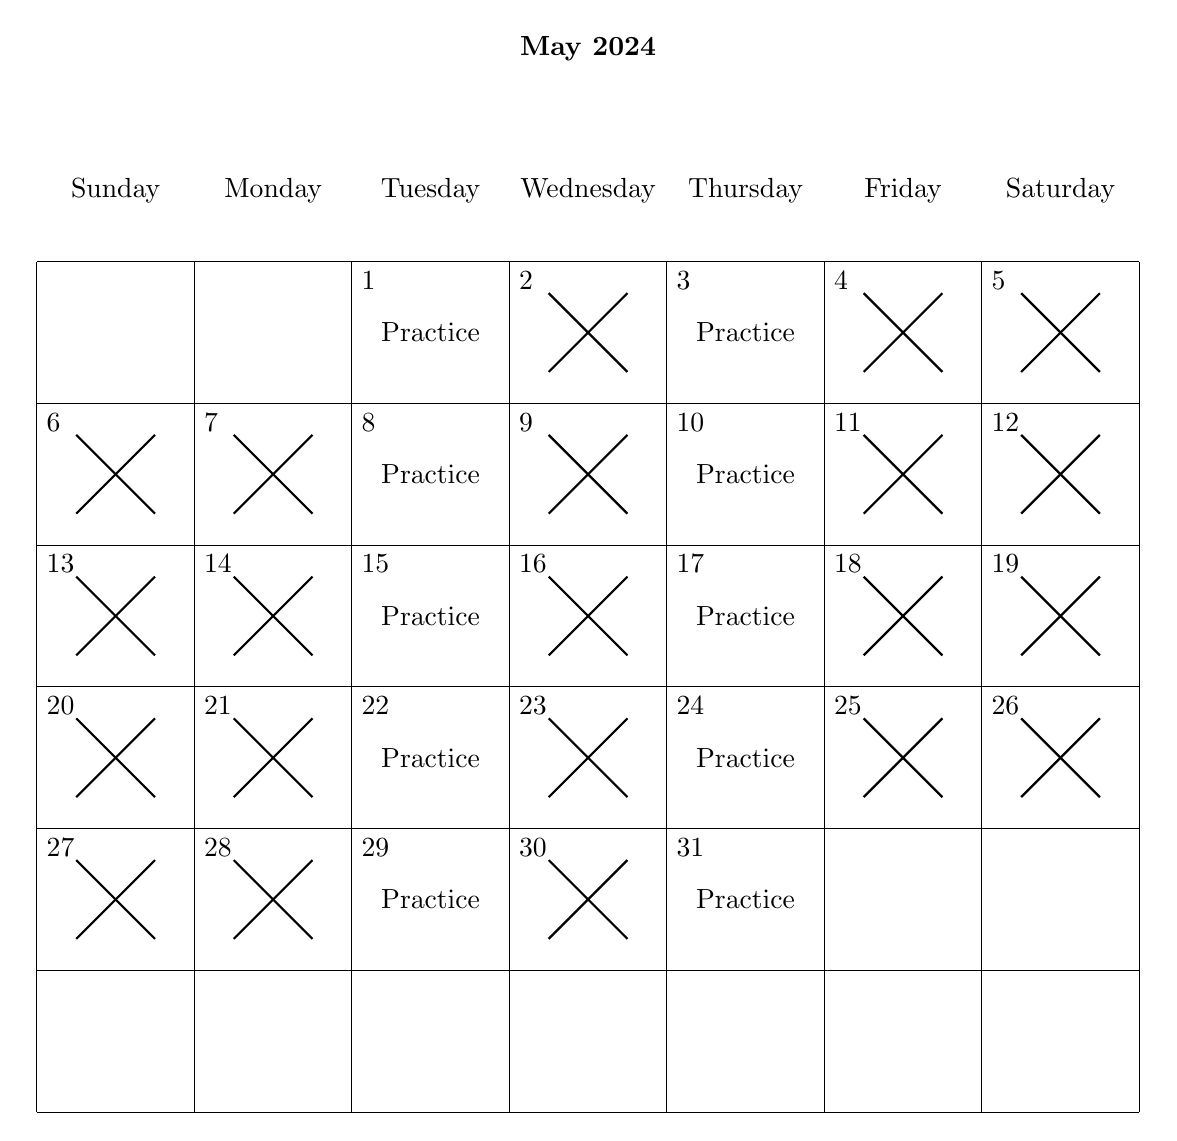
\begin{tikzpicture}
        % Define the dimensions of the calendar
        \def\year{2024}
        \def\month{5}
        \def\monthname{May}
        \def\startday{3} % 1=Sunday, 2=Monday, ..., 7=Saturday
        \def\numdays{31}
        \def\boxwidth{2} % Width of each box
        \def\boxheight{1.8} % Height of each box

\newcommand{\daytext}[1]{
    \ifcase#1
    \or Practice \or \cross \or Practice \or  \cross \or  \cross \or  \cross \or  \cross \or Practice \or  \cross \or Practice
    \or  \cross \or  \cross \or  \cross \or  \cross \or Practice \or  \cross \or Practice \or  \cross \or  \cross \or \cross
    \or  \cross \or Practice \or  \cross \or Practice \or  \cross \or  \cross \or  \cross \or  \cross \or Practice \or  \cross
    \or Practice
    \fi
}

        % Draw the calendar grid
        \foreach \x in {0, 1, 2, 3, 4, 5, 6, 7} {
            \draw (\x*\boxwidth, 0) -- (\x*\boxwidth, -6*\boxheight);
        }
        \foreach \y in {0, -1, -2, -3, -4, -5, -6} {
            \draw (0, \y*\boxheight) -- (7*\boxwidth, \y*\boxheight);
        }

        % Add day labels
        \node at (0.5*\boxwidth, 0.5*\boxheight) {Sunday};
        \node at (1.5*\boxwidth, 0.5*\boxheight) {Monday};
        \node at (2.5*\boxwidth, 0.5*\boxheight) {Tuesday};
        \node at (3.5*\boxwidth, 0.5*\boxheight) {Wednesday};
        \node at (4.5*\boxwidth, 0.5*\boxheight) {Thursday};
        \node at (5.5*\boxwidth, 0.5*\boxheight) {Friday};
        \node at (6.5*\boxwidth, 0.5*\boxheight) {Saturday};

        % Add the dates in the top left corner and specific text in the middle
        \foreach \d in {1,...,\numdays} {
            \pgfmathtruncatemacro{\col}{mod(\d+\startday-2, 7)}
            \pgfmathtruncatemacro{\row}{-(\d+\startday-2)/7}
            \node[anchor=north west] at (\col*\boxwidth, \row*\boxheight) {\d};
            \node[anchor=center, text width=\boxwidth cm, align=center] at (\col*\boxwidth+0.5*\boxwidth, \row*\boxheight-0.5*\boxheight) {\daytext{\d}};
        }

        % Add month and year
        \node at (3.5*\boxwidth, 1.5*\boxheight) {\textbf{\monthname\ \year}};
    \end{tikzpicture}
\end{center}

This is our what happened during the month of May. We had full team meetups every Tuesday and every Thursday. Connor had the robot during this time. At the end of the month we had just started building the Drivetrain.
\white{Team Biographies (May 2, 2024)}
\label{Team-Biographies}
\chapterauthor{Caleb Bachmeier}
\info{Caleb Bachmeier}{Team Biographies}{May 2, 2024}
\label{team-bios}
\textbf{Goal}: Breakdown the team's members

    \section*{7686X: Phoenix Rising}
    We are a VRC team out of Harrisburg, South Dakota. This year is our second second year competing as a team, in the 2023-2024 season we won the Innovate Award at South Dakota State Championship, while also making some excellent coding research which will be talked about later in this notebook.
   \section*{Connor Albers }
I am Connor Albers , this will be seventh year competing in VEX robotics, and I am in 10th grade at Harrisburg High School in Harrisburg South Dakota. I am the lead engineer of the robot.
\label{connor}
   \section*{Caleb Bachmeier}
I am Caleb Bachmeier, this will be my seventh year competing in VEX robotics,  and I am in 10th grade at Harrisburg High School in Harrisburg South Dakota. I am the team captain and document everything the team is doing in this engineering notebook. 
\label{Caleb}
   \section*{Miles Berger}
I am Miles Berger, this will be my seventh year competing in VEX robotics, and I am in 10th grade at Harrisburg High School in Harrisburg South Dakota. I am the backup driver for the team. 
\label{Miles}
   \section*{Chase Blake}
I am Chase Blake, this will be my fourth year competing in VEX robotics, and I am in 10th grade at Harrisburg High School in Harrisburg South Dakota. I am the main driver for the team but, when I am not driving, I research what other teams are doing to solve this year's challenge. 
\label{Chase}
   \section*{Ian Smith}
I am Ian Smith, this will be my second year competing in VEX robotics, and I am in 10th grade at Harrisburg High School in Harrisburg South Dakota. I am 1 of the 2 coders our team has and I mainly focus on integrating Jayden's code into the main drive program as well as finding the best ways for our driver to effectively control the robot. 
\label{Ian}
   \section*{Jayden}
I am Jayden, this will be my seventh year competing in VEX robotics, and I am in 10th grade at Harrisburg High School in Harrisburg South Dakota. I am 1 of the 2 coders our team has and I mainly focus on innovative ways our team can automate our robot. 
\label{Jayden}
\begin{center}
    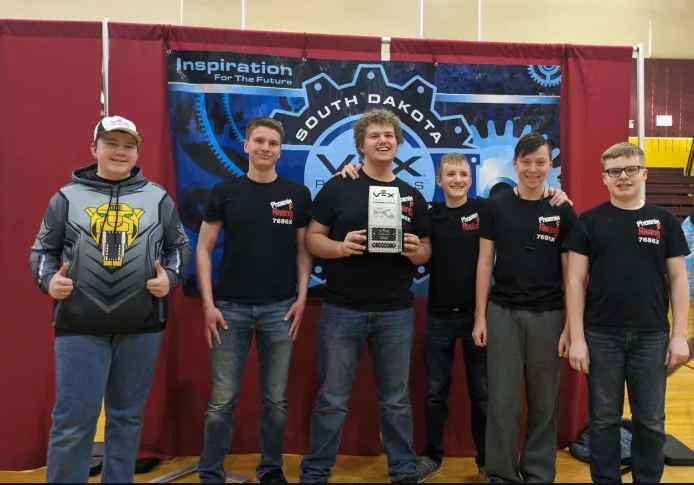
\includegraphics[width=0.9\linewidth]{images/Innovate wo Ezra.png}
    \captionof{figure}{Innovate at SD State} % Use \captionof instead of \caption
    \label{fig:innovate}
\end{center}

\white{Team Goals (May 5, 2024)}
\label{Team-Goals}
\chapterauthor{Caleb Bachmeier}
\info{Caleb Bachmeier}{Team Goals}{May 5, 2024}
{
\textbf{Goal}: Explain the team's goals for the High Stakes season
\section*{Team Goals}
\begin{itemize}
    \item \textbf{Learn something new}
    
    This might be our most important goal all season. Learning more is the only way to get better. We learned a lot last season through coding, building, driving, and notebooking. Even if it means we fail, learning not to make the same mistake twice is the best thing we can do.
    
    \item \textbf{Win a banner at a signature event}
    
    This would be an astounding achievement as banners at signature events are very hard to obtain. This would also make us much more appealing to future alliance partners, and they also look really neat.
    
    \item \textbf{Qualify for the World Robotics Competition }
    
    Qualifying for Worlds would be exceptional for the team. This has been a lifelong dream for us because it would allow us to show more teams what we can do. 
    
    \item \textbf{Win 85\% or more of qualification matches}
    
    This would place us higher in rankings. While it is an ambitious goal, the team thinks that it is one we should strive for, in order to get our name out there and hopefully gain better alliances in the future. 
    
    \item \textbf{Utilize all scoring methods of the game}
    
    When designing our robot, it is imperative to consider all approaches of the game. This will also help us better align ourselves with an alliance partner that compliments us best.

    \item \textbf{Be safe}

    Our safety goal is to operate our robot with precision and care. We commit to wearing safety glasses, respecting field boundaries, and avoiding unsafe actions. By prioritizing safety, we contribute to a positive and secure environment for all teams in the VEX VRC.
\end{itemize}
}
\white{Identify Game Problem (May 8, 2024)}
\label{Identify-Game-Problem}
\chapterauthor{Caleb Bachmeier}
\info{Caleb Bachmeier}{Identify Game Problem}{May 8, 2024}
\textbf{Goal}: Breakdown the High Stakes Game Manual Version 1.0
\section*{Field Analysis}
{
\textbf{Goal:} Analyze VEX VRC's game "High Stakes" (Figure \blueref{fig:high-stakes-field}{High Stakes Field})
\begin{itemize}
\item There are forty-eight rings on the field (Figure \blueref{fig:red-ring}{Ring Red})
\item Rings have an outer diameter of seven inches, inner diameter of three inches, and a thickness of two inches 
\item There are five hexagonal mobile goals on the field (Figure \blueref{fig:red-ring}{Ring Red}) 
\item Hexagonal mobile goals are ten inches wide and fourteen and a half inches tall
\item There are ten stakes you can score on, five hexagonal mobile goals, two alliance stakes, two wall stakes, and one stake on the four foot tall ladder 
\item On all stakes every ring is worth 1 point, except for the highest ring on the stake, which is worth three points
\item During the fifteen second autonomous period, you must stay on your alliances side.
\item Autonomous Win Point (AWP) is very useful for climbing up rankings as we have discovered in previous years
\item \hl{AWP at least three rings scored, two stakes with at least one ring scored.}
\item One robot can only carry two rings and one stake at a time. Rings scored on a goal that is being carried does not count against the two ring limit.
\item Rings can be descored at any time 
\item There is a four foot ladder in the middle of the field with three rings on it 
\item There are three levels on the ladder. Getting off of the ground gets you three points, passing above the first bar gets you six points, passing the second par gets you twelve points 
\item Robots can climb on any side of the ladder 
\item Between the four corners on the field, two are "positive corners" and the other two are "negative corners" teams can move mobile goals into these corners to change the scores on the mobile goals 
\item A positive corners multiplies the stakes points. For example, if I had a stake with six red rings on it, normally that stake would be worth 8 points, but if I put it into a positive corner, that stake would be worth 16 points, for the time that the stake is in the corner
\item A negative corner effectively makes the point values negative. For example, if I had a stake with six blue rings it would be worth an additional eight points for the blue alliance, but if I put that mobile goal into a negative corner, all points are negative and the mobile goal would be worth negative eight points for the blue alliance (Note: you can not have negative points at the end of the match, zero points is the lowest you can have)
\end{itemize}
\begin{figure}[hbt!] % Use [hbt!] to place the figures on the same page
    \begin{minipage}{.5\textwidth}
        \centering
        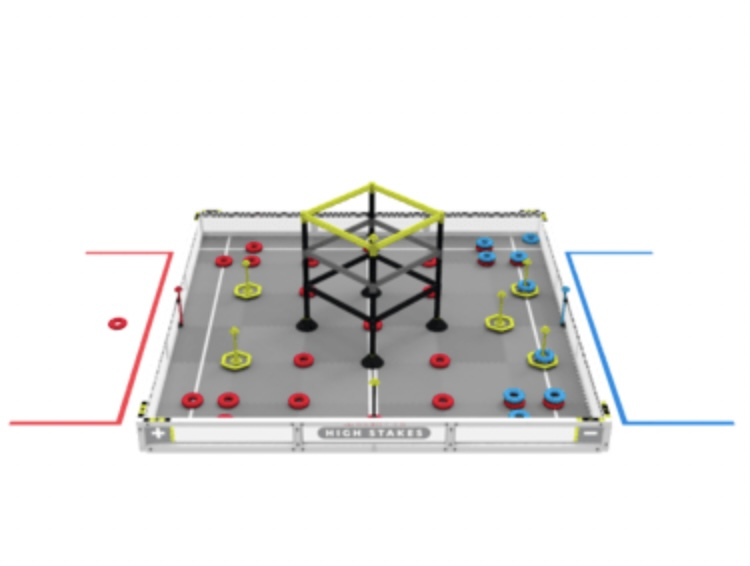
\includegraphics[width=.8\linewidth]{images/High Stakes Field.jpeg}
        \caption{High Stakes Field}
        \label{fig:high-stakes-field}
    \end{minipage}
    \begin{minipage}{.5\textwidth}
        \centering
        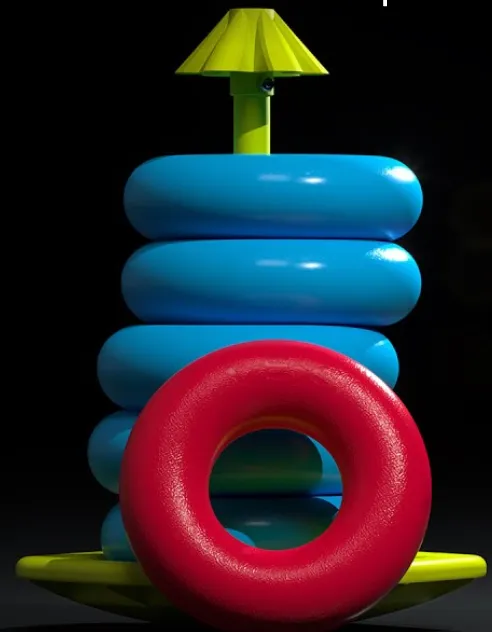
\includegraphics[width=.8\linewidth]{images/Stake.png}
        \caption{Mobile Goal with Rings}
        \label{fig:stake}
    \end{minipage}
    \begin{minipage}{.5\textwidth}
        \centering
        
\includegraphics[width=.8\linewidth]{images/Red Ring.jpeg}
        \caption{Red Ring}
        \label{fig:red-ring}
    \end{minipage}
\end{figure}
}
\section*{Important Terms}
    \subsection*{Game Objects}
    \begin{itemize}
    \item Rings (Figure \blueref{fig:red-ring}{Ring Red})
    \item Mobile Goals (Figure \blueref{fig:stake}{Stake})
    \end{itemize}
    \subsection*{Match Play}
    \begin{itemize}
        \item \textbf{Starting Line}: The location where robots are placed at the beginning of a match.
        \item \textbf{Autonomous Period}: A segment of the match where robots operate and score points using pre-programmed instructions without any driver input. This section of the match takes place in the first fifteen seconds of the match.
        \item \textbf{Driver Control}: This is the phase following the autonomous period where drivers control their robots to score points. This section of the match is ninety-five seconds long.
        \item \textbf{Endgame}: The final fifteen seconds of the match where teams can score additional points, often through specific tasks. This year by climbing a four foot tall ladder.
    \end{itemize}
    \subsection*{Violations}
    \begin{itemize}
\item \textbf{Minor Violation} - A Violation which does not result in a Disqualification

\item \textbf{Major Violation} - A Violation which results in a Disqualification

\item \textbf{Match Affecting} - A Violation which changes the winning and losing AllIance in the Match 

\item \textbf{Entanglement} - A Robot is Entangled if it has grabbed, hooked, or attached to an opposing Robot or a Field Element.

\item \textbf{Holding} - A Robot status, a robot is considered to be Holding if it meets any of the following criteria during match:
\begin{itemize}
    \item Trapping: Limiting the movement of an opponent Robot to a small or confined area of the field, approximately the size of one foam field tile or less, without any avenue for escape. \hl{(If a robot is not attempting to escape it is NOT trapped.)}
    \item Pinning: Preventing the movement of an opponent Robot through contact with the Field Perimeter, a Field or Game Element, or another Robot.
    \item Lifting: Controlling an opponent's movements by raising or tilting the opponents robot off of the foam tiles 
\end{itemize}
    \end{itemize}
\section*{Understanding Game Rules \vexManual}
%<SG> Rules 
{
\begin{itemize}
\item
\textbf{\textless SG1\textgreater} Starting a Match

- Prior to the start of each Match, the robot must be placed so that it is:
\begin{itemize}
    \item Contacting / breaking the plane of their Alliance's Starting Line
    \item Not contacting any scoring objects, with any exception of one Preload that is touching the robot
    \item Not contacting any other Robots 
    \item Completely stationary (i.e., no motors or any other mechanisms in motion)
\end{itemize}

- If an robot does not meet these requirements within a reasonable amount of time the robot is Disqualified from the match 
\item
\textbf{\textless SG2\textgreater} Horizontal expansion is limited

- Once the Match begins, Robots may expand outside of the 18" x 18" starting size, but the may never expand outside of the 24" x 18" size 

- From the robots perspective, it may only expand from one direction (from a single side of the robot)
\item
\textbf{\textless SG3\textgreater} Vertical expansion is limited

- Once the Match begins robots may expand vertically, but may never be breaking the plane of more than two Levels of the Ladder at any given time. \texthl{(This basically is a height limit of 32")} 
Game
- The floor is considered a Level 
\item
\textbf{\textless SG4\textgreater} Keep Scoring Objects in the field 

- Teams may not intentionally nor strategically remove Scoring Objects

- Any Rings that leave the Field during the Match will be given to the same Drive Team Members from the same color Alliance as the rings.
\item
\textbf{\textless SG5\textgreater} Each Robot gets one Ring as a preload 

- Prior to the start of the Match each preload must be contacting a robot of the same color as the preload 
\item
\textbf{\textless SG6\textgreater} Possession is limited to two Rings and one Mobile Goal

- If your robot has over this limit, it must stop all actions other than that of getting rid of the excess objects

- Rings on a mobile goal that you are carrying does not count against the ring count \texthl{(I.e. if your robot is carrying a mobile goal with six rings scored on it and is carrying two rings separately that would be legal.)}
\item
\textbf{\textless SG7\textgreater} Don't cross the Autonomous Line

- During the Autonomous period, Robots can not touch the foam tiles, Scoring Objects, or Field Elements which are on the opposing Alliance's side of the Autonomous Line \texthl{(Wall Stakes or Scoring Objects are on neither side of the line, both teams can come in contact with them)}

\item
\textbf{\textless SG8\textgreater} Engage with the Autonomous Line at your own risk 

- Any Robot who engages with Scoring Objects and/or the Wall Stakes on the Autonomous line should be aware that opponent Robots can do the same. 
\item
\textbf{\textless SG9\textgreater} Don't remove opponents from the ladder 

- There isn't a rule that explicitly states that incidental contact is prohibited; however, you can not intentionally pull a robot down from climbing 
\item
\textbf{\textless SG10\textgreater} Alliance Wall Stakes are protected

- Alliances can not directly nor indirectly interact with an opponent's Alliance Wall Stake. This includes Scoring and Descoring 
\item 
\subsection*{Update to Judging: June 26th}
\textbf{\textless SG11\textgreater} Positive corners are "safe" during the endgame

- During the last ten seconds of a Match, Robots may not contact Mobile Goals in the Positive Corners of the Field, and may not add or remove Mobile Goals or Rings to or from the Positive Corners of the field
\end{itemize}
}
\white{Game Strategies (May 10, 2024)}
\label{Game-Strategies}
\chapterauthor{Chase Blake}
\info{Chase Blake}{Game Strategies}{May 10, 2024}
\textbf{Goal}: Identify offensive and defensive game strategies
    \section*{Game Strategy}
    \textbf{Goal}:
    We will develop game strategies for this year's game so that we can have a better understanding of what we may encounter in game

    \textbf{Scoring Prioritization}:
    Admittedly, this is going to be a very odd year for scoring because of the positive and negative corners. We will count negative points against our opponents as positive points for us.

    \textbf{Scoring Method Points}:
    \begin{itemize}
        \item Eight points for a fully stacked stake
        \item Sixteen points for a fully stacked stake in any of the corners 
        \item Three points for getting off of the ground using the ladder 
        \item Six points for passing the first rung of the ladder
        \item Twelve points for passing the second rung of the ladder 
    \end{itemize}
    \centering \textbf{On the following page there is a bar graph of point breakdown}
    \pagebreak
    \begin{figure}[t!]
        \centering
        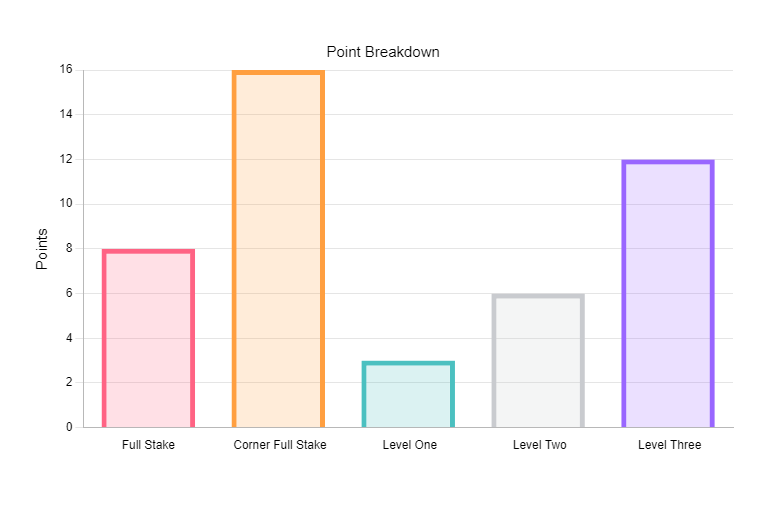
\includegraphics[width=1\textwidth]{images/Point Breakdown .jpg}
        \caption{Point Breakdown}
        \label{fig:point-breakdown}
    \end{figure}
    
    \section*{Offensive Strategies}
\noindent
    \textbf{Defending a full stake in the negative corner}:

\noindent
\textbf{Pros}:
\begin{itemize}
    \item Guaranteed negative eight points for the opposing alliance 
\end{itemize}
\textbf{Cons}:
\begin{itemize}
    \item Loses out on all other opportunities to score points 
\end{itemize}

    \textbf{Descoring opponent's stakes}:

\noindent
\textbf{Pros}:
\begin{itemize}
    \item Makes the opponents attempts to score futile 
\end{itemize}
\textbf{Cons}:
\begin{itemize}
    \item Loses out on other opportunities to score points 
\end{itemize}
    \section*{Defensive Strategies}
    \noindent
    \textbf{Hanging as soon as possible}:

\noindent
\textbf{Pros}:
\begin{itemize}
    \item Guaranteed Twelve Points for a Level 3 hang
\end{itemize}
\textbf{Cons}:
\begin{itemize}
    \item Loses out on other opportunities to score additional points 
\end{itemize}

\noindent
    \textbf{Defending a full stake in the additional corner}:

\noindent
\textbf{Pros}:
\begin{itemize}
    \item Guaranteed Sixteen Points 
\end{itemize}
\textbf{Cons}:
\begin{itemize}
    \item Loses out all opportunities to score additional points 
\end{itemize}

\noindent
    \textbf{Defending a stake, then hanging at the end of the match}:

\noindent
\textbf{Pros}:
\begin{itemize}
    \item If us and our allIance partner does this a point maximum is 56 points
\end{itemize}
\textbf{Cons}:
\begin{itemize}
    \item High risk, high reward. If when we leave to go hang one of our opponents goes to descore our stakes the bulk of our points would be lost  
\end{itemize}
\white{Gantt Chart (May 13, 2024)}
\label{Gantt-Chart}
\chapterauthor{Caleb Bachmeier}
\info{Caleb Bachmeier}{Gantt Chart}{May 13, 2024}
\textbf{Goal}: Identify our timeline for the High Stakes season
\section*{Gantt Chart: May 2024 - October 2024}

    The Gantt Chart below (\blueref{may-gantt-chart}{May Gantt Chart}) covers the time frame from May of 2024 (the beginning of our season) to October of 2024. These are our goals for the season. Our biggest goal is finishing our first robot by the end of July, this will allow for about  three months of drive time for our drivers, \blueref{Chase}{Chase} and \blueref{Miles}{Miles}, before our first tournament which will be in October
\begin{figure}[H]
    \begin{center}
        \begin{ganttchart}[
            y unit title=0.4cm,
            y unit chart=0.5cm,
            vgrid,
            hgrid,
            title label anchor/.style={below=-1.6ex},
            title left shift=.05,
            title right shift=-.05,
            title height=1,
            progress label text={},
            bar height=0.7,
            group right shift=0,
            group top shift=.6,
            group height=.3
        ]{1}{24} % Number of weeks
            % Labels
            \gantttitle{Week}{24} \\
            \gantttitle{May}{4}
            \gantttitle{June}{4}
            \gantttitle{July}{4}
            \gantttitle{August}{4}
            \gantttitle{September}{4}
            \gantttitle{October}{4}\\
            % Tasks
            \ganttbar{Set Up}{1}{2} \\
            \ganttbar{Build 1st Robot}{3}{12} \\
            \ganttbar{Program 1st Robot}{8}{12} \\
            \ganttbar{Improve 1st Robot}{13}{24} \\
            \ganttbar{Drive 1st Robot}{13}{24} \\
            % Relations \ganttlink{elemx}{elemy}

        \end{ganttchart}
    \end{center}
    \caption{Gantt Chart}
    \label{may-gantt-chart}
\end{figure}
\pagebreak
\section*{Gantt Chart: November 2024 - April 2025}

    The Gantt Chart below (\blueref{november-gantt-chart}{November Gantt Chart}) covers the time frame from November of 2024 to April of 2025 (the end of our season). Our main goal is to finish building our second robot by New Years. This will ensure that our robot will be ready to be driven to prepare for the rest of our qualification tournaments. Our third robot will be our state tournament, U.S. Open, and our Worlds robot. 
    \begin{figure}[H]
    \begin{center}
        \begin{ganttchart}[
            y unit title=0.4cm,
            y unit chart=0.5cm,
            vgrid,
            hgrid,
            title label anchor/.style={below=-1.6ex},
            title left shift=.05,
            title right shift=-.05,
            title height=1,
            progress label text={},
            bar height=0.7,
            group right shift=0,
            group top shift=.6,
            group height=.3
        ]{1}{24} % Number of weeks
            % Labels
            \gantttitle{Week}{24} \\
            \gantttitle{November}{4}
            \gantttitle{December}{4}
            \gantttitle{January}{4}
            \gantttitle{February}{4}
            \gantttitle{March}{4}
            \gantttitle{April}{4}\\
            % Tasks
            \ganttbar{Improve 1st Robot}{1}{8} \\
            \ganttbar{Drive 1st Robot}{1}{8} \\
            \ganttbar{Build 2nd Robot}{1}{8} \\
            \ganttbar{Program 2nd Robot}{4}{10} \\
            \ganttbar{Improve 2nd Robot}{8}{13} \\
            \ganttbar{Drive 2nd Robot}{8}{13} \\
            \ganttbar{Build Final Robot}{10}{16} \\
            \ganttbar{Improve Final Robot}{16}{24} \\
            \ganttbar{Drive Final Robot}{16}{24} \\
        \end{ganttchart}
    \end{center}
    \caption{Gantt Chart}
    \label{november-gantt-chart}
    \end{figure}
\white{Skills Rules (May 14, 2024)}
\label{skills-rules}
\chapterauthor{Miles Berger}
\info{Miles Berger}{Skills Rules}{May 14, 2024}
\section*{Overview of VEX Skills}
The VEX Robotics Competition (VRC) includes a variety of challenges designed to test the skills and creativity of participants. One of the key components is the Robot Skills Challenge, which consists of two parts: Driver Skills and Programming Skills. In Driver Skills, the robot is controlled by a driver to score as many points as possible within a set time. In Programming Skills, the robot operates autonomously using pre-written code to achieve the highest score possible. These challenges encourage students to develop their programming and driving skills, as well as their strategic thinking and problem-solving abilities.

\section*{High Stakes Season Skills Rules}
The High Stakes season introduces several unique changes to the Skills Challenge rules compared to previous seasons. One of the most notable differences is the new field layout, where Positive Corners and Negative Corners are now on the same side of the field, rather than being cater-cornered. This change affects the strategy for both Driver Skills and Programming Skills, as teams must now navigate the field differently to maximize their scoring potential. Additionally, the High Stakes season includes a new rule that adds a 2-point bonus per Climb for whichever alliance has Rings scored on the High Stake at the end of a match. This incentivizes teams to focus on scoring Rings on the High Stake, adding a new layer of complexity to the Skills Challenge.

Another significant change is the clarification and expansion of several existing rules. For example, the definition of "Plowing" has been rewritten, and new figures have been added to clarify the intent of specific rules. The rules for preloads have also been updated to ensure that they cannot start in a scored location or in contact with Stakes. These changes aim to provide clearer guidelines and prevent any ambiguities that could affect the outcome of matches. Overall, the High Stakes season's Skills Challenge rules emphasize strategic planning and precise execution, making it a more challenging and engaging competition for teams.

\section*{Scoring Rules for Red and Blue Rings}
In the High Stakes season, the scoring rules for red and blue rings have been updated to add more strategic depth to the game. Each ring scored on a stake is worth one point, while the top ring on each stake is worth three points. Additionally, mobile goals can be placed into Positive Corners or Negative Corners to change the values of the rings on that goal. This means that teams must carefully plan their ring placements to maximize their scores.


Furthermore, the rules specify that for a blue ring to have a point value in any position, all 24 red rings must be scored on stakes and have point values at the end of the match. This adds an extra layer of complexity, as teams must ensure that all red rings are properly scored before blue rings can contribute to their total score. These changes encourage teams to develop more sophisticated strategies and enhance the overall challenge of the Skills Competition.

\begin{figure}[!ht]
    \centering
    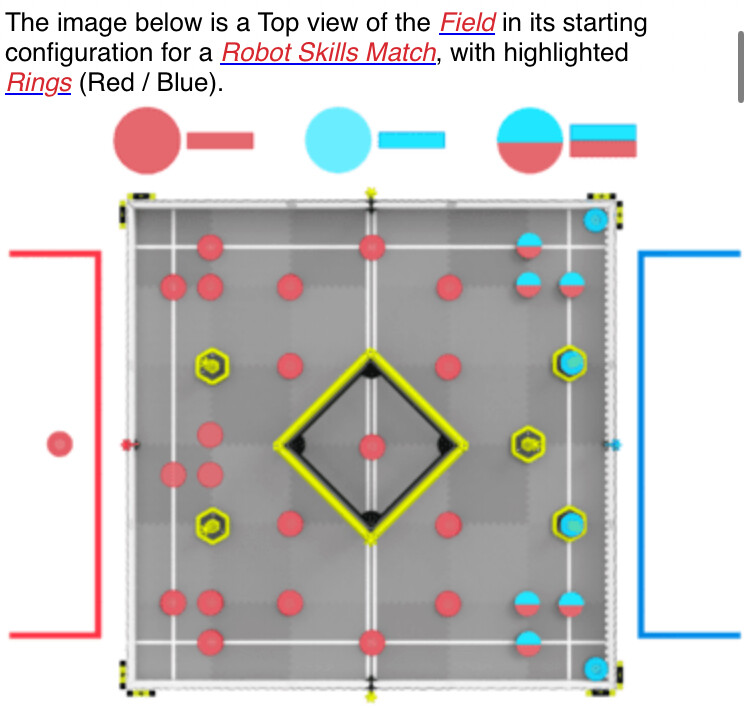
\includegraphics[width=0.5\linewidth]{images/SkillsFieldHighStakes.jpeg}
    \caption{Skills Field}
    \label{fig:skillsfield}
\end{figure} %May 14 
\white{Programming (May 15, 2024)}
\label{Programming}
\chapterauthor{Ian Smith}
\info{Caleb Bachmeier}{Programming}{May 15, 2024}
\textbf{Goal}: Explain Ian's programming work

\section*{Introduction}
The challenges of this year's game require a unique and nuanced approach to programming. While traditional programming remains largely similar to previous years, skills programming is significantly different due to the placement of game objects and the scoring requirements.

\section*{Skills Rules}
Skills Rules are explained in detail in the previous chapter: \blueref{skills-rules}{Skills Rules}
\section*{Programming Skills Challenges}
Some of the most unique challenges, after analyzing programming skills challenges, are the requirements to create a program that can list all the ways to earn skills points.

\section*{Proposed Solutions}
Some of the proposed solutions included using standard programming techniques with basic VEX functions similar to previous years, employing a repeating program developed by Ian in earlier seasons, implementing LemLib for PID and Pure Pursuit control, utilizing AI for autonomous control, and combining LemLib with AI. Due to the potentially significant rewards of the last option, that approach was ultimately developed.

\section*{AI Development}
Ian's AI development is explained in full detail in chapter \blueref{Artificial-Intelligence-Library}{Artificial Intelligence Library}

\section*{General Match Control}
In terms of general match control, several key points have emerged so far this season: a HUD for the robot brain and options for improved control.

\section*{Control System}
After testing curvature drive and arcade drive with our driver(s), we determined that curvature drive offers better control. The concept of curvature drive allows the robot to follow a fixed radius curve based solely on the steering stick, eliminating reliance on velocity like arcade drive.

\section*{HUD Design}
For HUD design, several concepts were considered, including an interactive terminal and interactive menus. Due to the simplicity of the menus and their ease of programming, that option was chosen.

\section*{Programming Software}
All programming is conducted on Ubuntu, as it was the system I had available. The PROS software was the obvious choice over the VEX V5 name-space and compiler due to its closer adherence to C standards and versatile features.
\begin{comment}
\white{Fusion 360 (May 16, 2024)}
\label{Robot-CAD}
\chapterauthor{Connor Albers }
\info{Caleb Bachmeier}{Fusion}{May 16, 2024}
\textbf{Goal}:
    \section*{Robot CAD}
\end{comment}
\important{CNC Machining Research (May 17, 2024)}
\label{CNC-Machining}
\chapterauthor{Ian Smith}
\info{Ian Smith}{CNC Machining}{May 17, 2024}


\textbf{Goal}: Explain the team's CNC machining research

% CNC Machining Research
\section*{CNC Machining (Research)}

% Introduction and Background
\subsection*{Introduction and Background}
After brief experimentation last year with using primitive (mostly “eyeballing”) methods of custom parts manufacturing and “machining” —used very loosely,— we have decided to take advantage of the resources available to us. Fortunately, our team coach, Paul, is a hobbyist machinist with a relatively diverse range of tooling. Among the tools are mills, lathes, and a 4-axis CNC mill. However, to maintain VEX legality, a few rules must be followed.

% VEX Legality
\subsection*{VEX Legality}
Because of rule \textless R2\textgreater, it has to be members of our team doing the machining. This includes all CAD, tool-path generation, G and M code generation, calculations, and machining operations.

Machining (including CNC) is legal because it is subtractive manufacturing and is only modifying the VEX part, which is legal per rule \textless R16\textgreater: "Physical modifications, such as bending or cutting, of legal metal structure or plastic components are permitted.".

% Resources and Stock
\subsection*{Resources and Stock}
Primarily, as resources for the project, we used suggestions from our coach along with the \textit{Machinist’s Handbook}. Regarding our “stock,” we are relatively limited, with only high-strength axles (SKU 276-7465) and 24-tooth gears (SKU 276-7572) making convenient stock. High-strength axles are synonymous with Zinc Galvanized ¼ inch Square Stock with a maximum length of 24 inches. The 24-tooth gears are synonymous with 0.9-inch diameter round stock with a maximum length of ½ inch. Both parts are assumed to be 1045 mild steel based on what we found on the VEX website. Overall, the material is quite limiting, but we are still capable of making custom small-space mechanisms. One of the theorized applications of machined parts was custom gearing through better build mechanisms such as steel helical gears with custom ratios. 

% Research and Calculations
\subsection*{Research and Calculations}
When researching the stock to find relevant information, I started by going to McMaster-Carr to find the corresponding square stock (\href{https://www.mcmaster.com/8962K33/}{This is a link to McMASTER-CARR}). Afterward, I found a stress-strain graph for the alloy to perform calculations on the material when engineering custom parts (\href{https://www.mdpi.com/2073-4352/13/8/1287}{This is a link to the project page}
\textcite{cryst13081287}).

\begin{figure}[H]
    \centering
    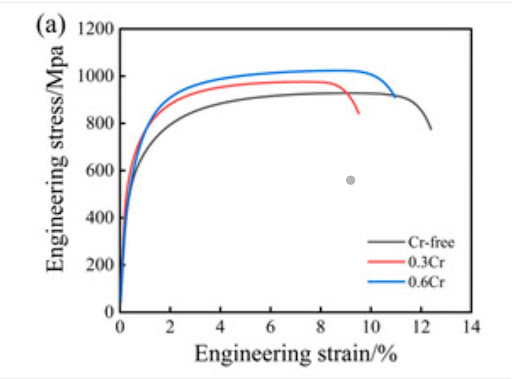
\includegraphics[width=0.5\linewidth]{images/CNC Machining Graph.jpg}
    \caption{Engineering Strain \%}
    \label{fig:cnc-machining-graph}
    \cite{cryst13081287}
\end{figure}

After interpreting the graph, we observed a yield point at about 800 MPa/mm\(^2\). After discussion, we decided to maintain a factor of safety around 1.5, or aircraft grade. This was decided because we don’t need longevity; we need short bursts of performance from our parts. The only downside to that low of a factor of safety is the occasional extreme forces our robots may be subjected to during a match. The most likely stress we will have to engineer around is shear force. For our stress calculations on parts, we plan on using the tool within Fusion 360, which we use to design the bot for construction, testing, and simulation.

\section*{Clarification on Legality}\footnote{Added: November 18, 2024}

At our North Dakota Signature Event, despite the repetitive clarifications on legality, we were still questioned about rule violations. As a solution to this problem, we were posed with a few different solutions. We could go back and edit the original entry. We could clarify in a different entry. We could add an FAQ to the original entry. We decided to go with the last option because of the clarity and simplicity. 

\begin{itemize}
    \item \textbf{Are you using non-VEX legal parts?} \\
    No, we are not using non-VEX parts. We actually haven’t bought a part to machine yet.
    
    \item \textbf{Have you machined a part yet?} \\
    No, we have not machined a part yet, we technically haven’t bought stock yet.
    
    \item \textbf{Based on this research, how did you derive material type?} \\
    Experience outside of VEX. The 1045 Low Carbon Steel comes directly from the VEX Website "\cite{vexRobotics}", which is backed up by \textit{\textit{Machinery’s Handbook} "\cite{machinists}."} "\cite{machinists}." The Zinc/Chromium plating comes from assumed corrosion resistance and the shiny material on the outside of the shaft.
    
    \item \textbf{Why are you citing an outside purchasing source (McMaster-Carr)?} \\
    Before I knew \textit{Machinery’s Handbook} "\cite{machinists}." existed, I took the information I knew about material science and also knew that I didn’t have enough information to do full stress calculations. I just went onto a third-party source and looked for ¼ inch 1045 square stock. Because of VEX’s lack of information and my not owning a copy of \textit{Machinery’s Handbook} "\cite{machinists}." yet, I had to go to an outside source for research purposes only.
    
    \item \textbf{How will you document the work process?} \\
    We plan on recording the process of writing the G and M codes, documenting the math used before the operations, and recording the actual machining. On the condition that we are asked by a Judge or Referee at an event, our goal is to be able to show undisputable evidence that everything we did was completely legal.
\end{itemize}

In conclusion, this short FAQ was intended to show that the chapter was written as research only and we always have purchased legal parts.
 %May17
\white{Pneumatics (May 20, 2024)}
\label{Pneumatics}
\chapterauthor{Caleb Bachmeier}
\info{Caleb Bachmeier}{Pneumatics}{May 20, 2024}
\textbf{Goal}: Explain the VEX V5 Pnuematic system, and how we could use it for our robot this season.
\section*{Overview of VEX V5 Pneumatics}

Pneumatics in the VEX Robotics Competition (VRC) involve the use of compressed air to create mechanical motion. VEX V5 pneumatics systems allow robots to perform various tasks such as lifting, grabbing, or moving objects with precise control. These systems can be particularly useful in achieving tasks quickly and with less motor usage, which can be advantageous given the limited number of motors allowed in VEX competitions.

\section*{Components of a VEX V5 Pneumatics System}

\begin{itemize}
    \item \textbf{Pneumatic Cylinders}: Convert compressed air into linear motion. Available in different sizes and stroke lengths.
    \item \textbf{Solenoid Valves}: Control the flow of air into and out of the cylinders. Available in single-acting and double-acting types.
    \item \textbf{Air Reservoir}: Stores compressed air that powers the pneumatic system.
    \item \textbf{Tubing and Fittings}: Connect the various components, allowing air to flow through the system.
    \item \textbf{Pressure Regulator}: Controls the pressure of the air supplied to the system, ensuring safe and functional limits.
    \item \textbf{Pump}: Manual or electric pump used to initially fill the air reservoir with compressed air.
\end{itemize}
\centering \textbf{}
\begin{figure}[hbt!] % Use [hbt!] to place the figures on the same page
    \begin{minipage}{.5\textwidth}
        \centering
        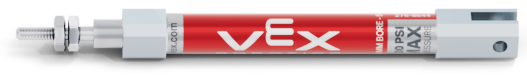
\includegraphics[width=.8\linewidth]{images/Double Action Pneumatic Piston.png}
        \caption{Double Action Cylinder}
        \label{fig:double-action-pneumatic-piston}
    \end{minipage}
    \begin{minipage}{.5\textwidth}
        \centering
        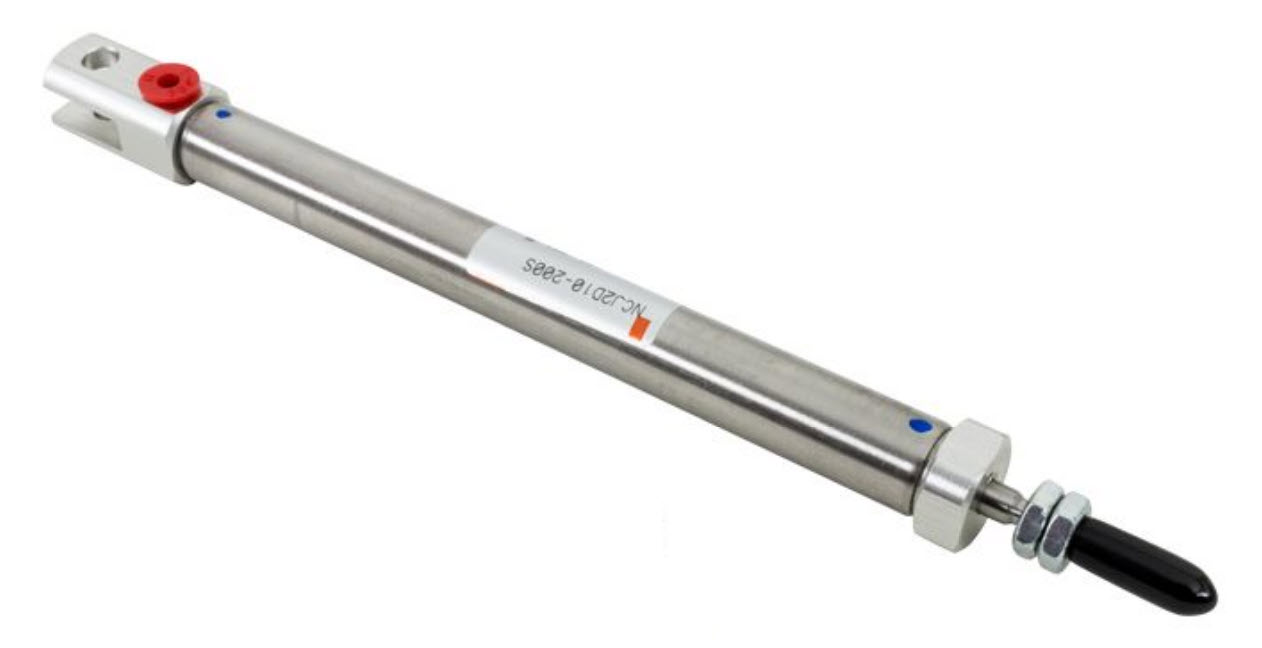
\includegraphics[width=.8\linewidth]{images/Single Action Cylinder.jpg}
        \caption{Single Action Cylinder}
        \label{fig:single-action-cylinder}
    \end{minipage}
    \begin{minipage}{.5\textwidth}
        \centering
        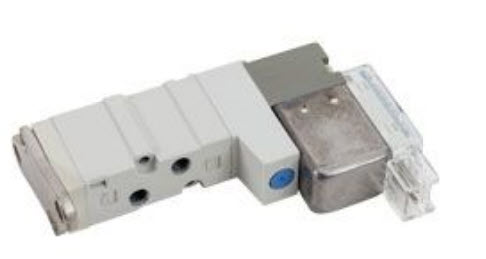
\includegraphics[width=.8\linewidth]{images/Solenoid.jpg}
        \caption{Solenoid}
        \label{fig:solenoid}
    \end{minipage}
    \begin{minipage}{.5\textwidth}
        \centering
        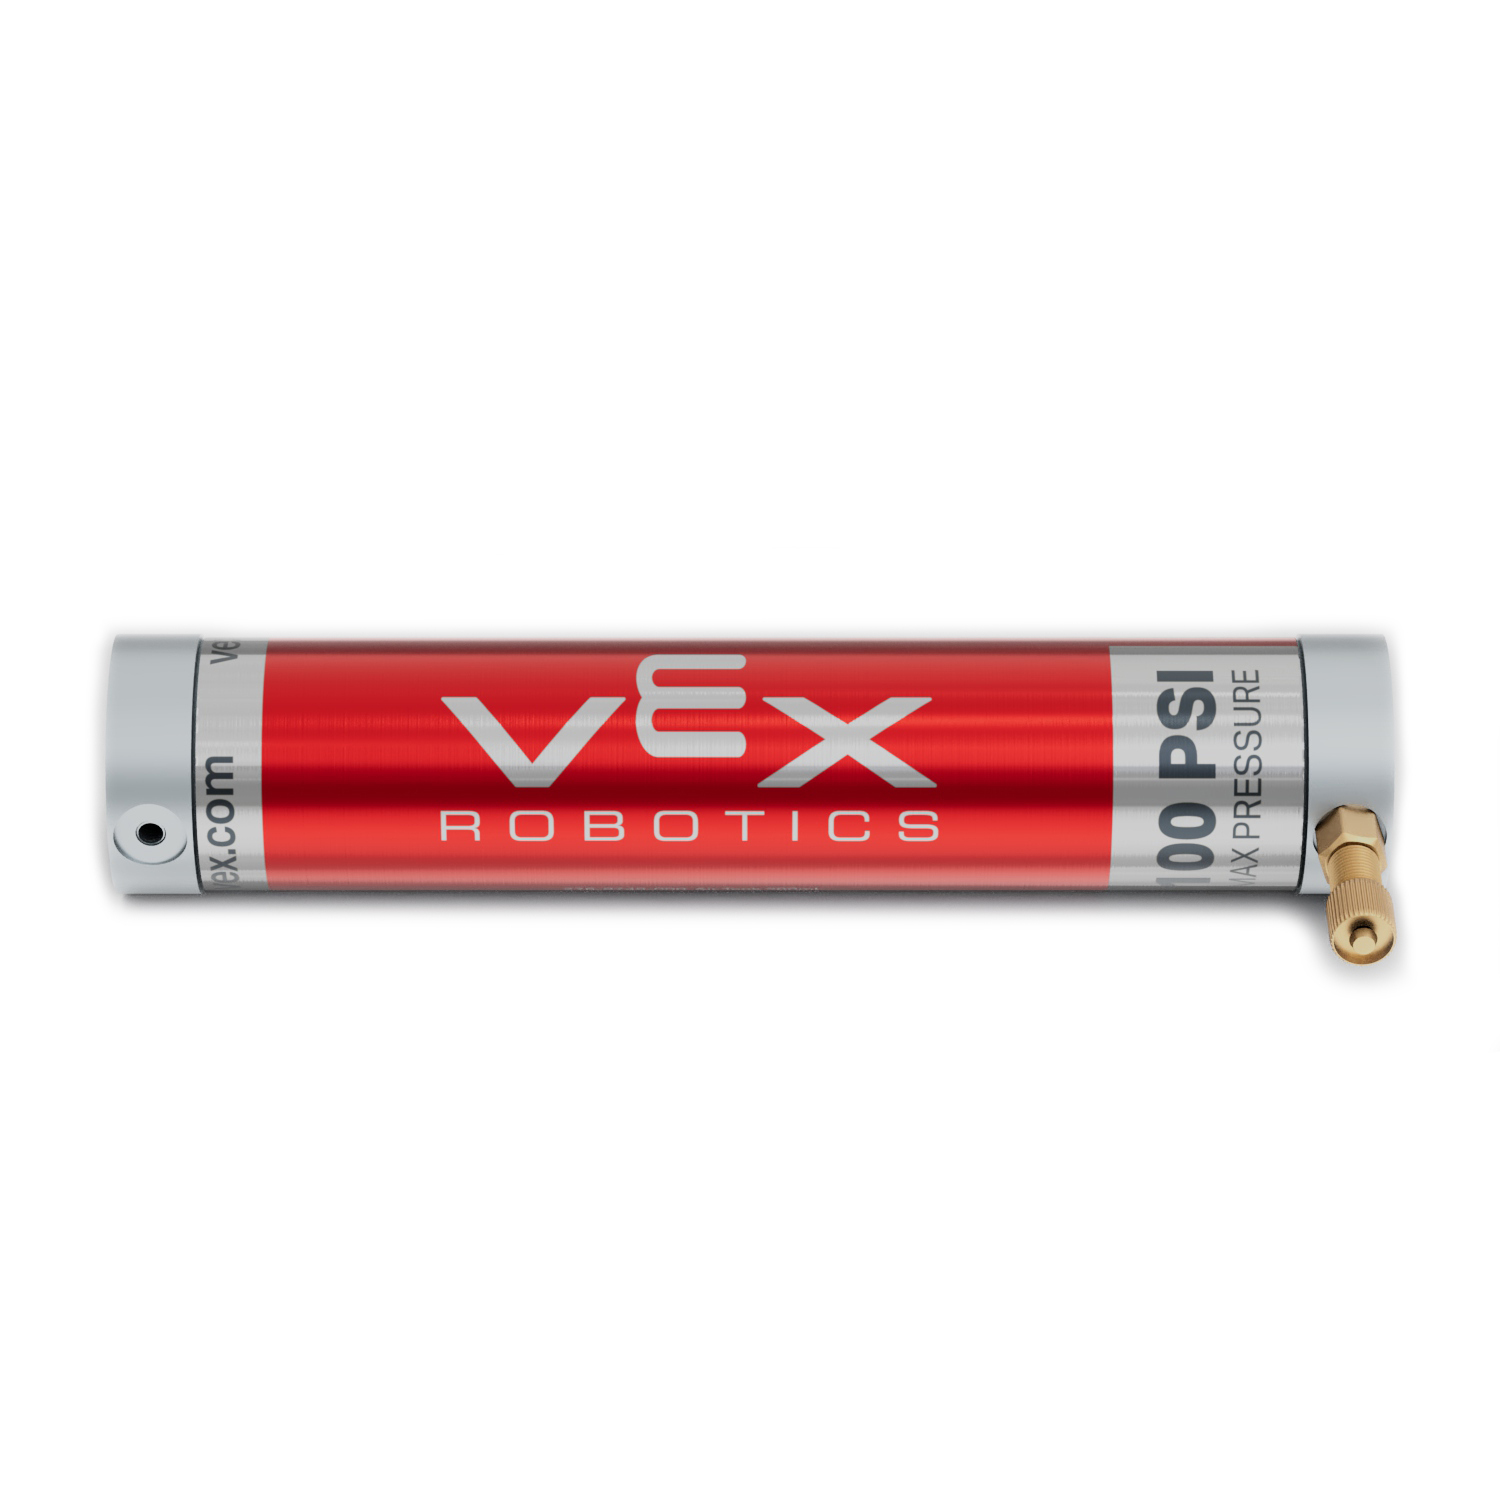
\includegraphics[width=.8\linewidth]{images/Air Resivoir.png}
        \caption{Air Reservoir}
        \label{fig:air-reservoir}
    \end{minipage}
        \begin{minipage}{.5\textwidth}
        \centering
        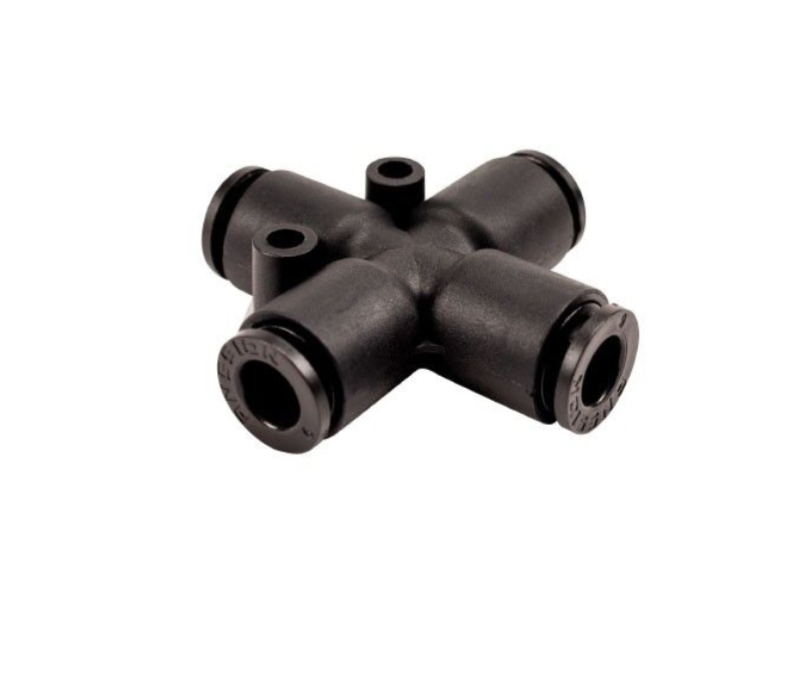
\includegraphics[width=.8\linewidth]{images/Fittings.jpeg}
        \caption{Fittings}
        \label{fig:fittings}
    \end{minipage}
        \begin{minipage}{.5\textwidth}
        \centering
        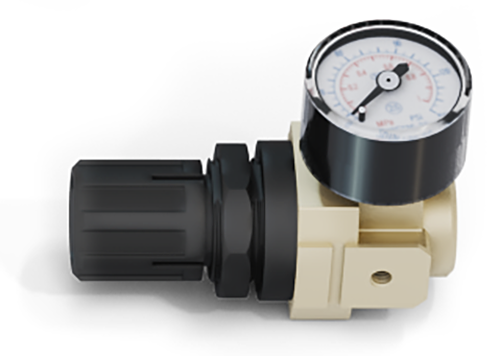
\includegraphics[width=.8\linewidth]{images/Pressure Regulator.png}
        \caption{Pressure Regulator}
        \label{fig:pressure-regulator}
    \end{minipage}
\end{figure}

\pagebreak
\section*{Advantages and Disadvantages of Pneumatics}

\subsection*{Advantages}

\begin{itemize}
    \item \textbf{Quick Actuation}: Provides faster actuation compared to motors, allowing for quicker response times.
    \item \textbf{Strong Force}: Generates significant force, useful for tasks requiring high power, like lifting heavy objects.
    \item \textbf{Efficiency}: Reduces the load on motors, advantageous given the motor limits in VEX competitions.
    \item \textbf{Precision}: Provides precise and repeatable motion, beneficial for tasks requiring accuracy.
    \item \textbf{Motor Maximum}: Pneumatics do not count towards our 88 watt motor limit
\end{itemize}

\subsection*{Disadvantages}

\begin{itemize}
    \item \textbf{Limited Air Supply}: Once the air in the reservoir is depleted, the system requires recharging, limiting usage during matches.
    \item \textbf{Complexity}: Adds complexity to the robot design and requires careful planning and maintenance.
\end{itemize}

\section*{Strategic Use in the 24-25 High Stakes Season}

Effective use of pneumatics could significantly enhance our robot's performance for the 24-25 VEX VRC High Stakes season. Here are some strategic applications:

\subsection*{Claw Mechanism}
Using pneumatic cylinders to operate a claw for grabbing and releasing objects quickly and with high force.

\subsection*{Lifting Mechanism}
Implementing a pneumatic lift to raise and lower objects rapidly, beneficial for stacking tasks or reaching high goals.

\subsection*{Endgame Tasks}
Designing pneumatic mechanisms specifically for endgame tasks that require fast and powerful actuation, such as deploying scoring elements or expanding the robot to control areas.

\subsection*{Multi-Functionality}
Creating mechanisms that can perform multiple functions, such as a single pneumatic system that can both lift and grab, reducing the need for additional motors.

\section*{Example Design: Pneumatic Claw and Lift System}

\subsection*{Claw Design}
Use two double-acting pneumatic cylinders for the claw to provide strong and reliable gripping force. Control the cylinders with solenoid valves, allowing precise control over the opening and closing of the claw.

\subsection*{Lift Design}
Implement a scissor lift or a linear slide mechanism powered by pneumatic cylinders. Use a pressure regulator to ensure the lift operates within safe pressure limits and to control the speed of the lift.

\subsection*{Integration}
Connect the claw and lift to a single air reservoir to save space and weight. Use a manual pump to recharge the reservoir between matches, ensuring the system is always ready for maximum performance.

\subsection*{Control System}
Program the VEX V5 brain to control the solenoid valves based on input from sensors and user commands. Use limit switches or potentiometer to provide feedback on the position of the claw and lift, allowing for precise control.

\section*{Equations}

\subsection*{Equation for Linear Force}
The equation for the ideal linear force generated by a pneumatic cylinder is:
\[
\text{Ideal Linear Force} = \pi \left( \frac{\text{B}_\text{in}}{2} \right)^2
\]
In which:
\begin{itemize}
    \item \textbf{B} is the bore of the pneumatic cylinder (the diameter of the cylinder's internal chamber).
\end{itemize}

This equation calculates the cross-sectional area of the bore, which is then multiplied by the pressure to determine the force exerted by the pneumatic cylinder.

\subsection*{Equation for Volume Reduction per Stroke}
The equation for the volume reduction per stroke of a pneumatic system is:
\[
\Delta V = \left(\frac{\text{B}_\text{in}}{2}\pi \right)^2 \cdot \text{stroke}_\text{in} + \left(\frac{\text{tube cross-section}_\text{in}}{2}\pi \right)^2 \cdot \text{tube length}_\text{in}
\]
In which:
\begin{itemize}
    \item \textbf{B} is the bore of the pneumatic cylinder.
    \item \textbf{Stroke} is the distance the piston travels within the cylinder.
    \item \textbf{Tube Cross-section} is the diameter of the tubing connected to the pneumatic cylinder.
    \item \textbf{Tube Length} is the length of the tubing connected to the pneumatic cylinder.
\end{itemize}

This equation calculates the total volume reduction in the pneumatic system when the piston moves through its stroke. The first term represents the volume change in the cylinder, and the second term represents the volume change in the tubing.

In order to calculate total volume of the system at an given point in time, a basic formula can be derived. By starting with the combined gas law: \[\frac{V_1\cdot P_1}{T_1} = \frac{V_2\cdot P_2}{T_2}\]
\begin{itemize}
    \item \textbf{v} is the volume at a given interval
    \item \textbf{p} is the pressure of the system at a given interval
    \item \textbf{t} is the temperature in degrees kelvin at a given interval
\end{itemize}
In our example, temperature is assumed to be constant, giving the formula: \[V_1\cdot P_1 = V_2\cdot P_2\]
Using algebra to solve for $P_2$... \[P_2 = \frac{V_1\cdot P_1}{V_2}\]
And plugging it into a usable formula for residual computation... \[P_n = \frac{P_{n-1}\cdot V}{V + \Delta V}\]

\subsection*{Real-Time Computation (Added October 15, 2024)}

In order to calculate or air pressure mid match, we need a couple of known variables. 
\begin{itemize}
    \item The total volume of the system $(V)$.
    \item The volume of each section of the system after a solenoid that could be cycled, referred to as $(\Delta V)$.
    \item The initial pressure $(P_1)$ of the pneumatic system (what we set it to at the beginning of the match).
\end{itemize}
While our team could set our pneumatic to any pressure between 0 and 100 (per rule \textless R23\textgreater, clause b: Pneumatic devices may be charged to a maximum of 100 psi.), we do have an experimentally determined minimum of about \(50\text{psi}\). We could calculate a precise minimum based on the force exerted and required by each mechanism, but this is not strictly necessary and is much easier to determine experimentally. It makes sense the most amount of sense to use $100psi$ as our initial \(P_1\) value as per the formulation in the last chapter higher a \(P_1\) provides the most amount of cycles.

%caleb pls fix this. Also, add that it was added in at a later date.

When designing the software for residual pressure computation, I originally came up with three (3) initial solutions. 
\begin{itemize}
    \item Brute force within the \begin{verbatim}
        opcontrol()
    \end{verbatim} loop.
    \item Set a function for volume calculations for each possible action.
    \item Create classes for each type of component that can store volume, subsystems, and the system as a whole.
\end{itemize}
The advantage of using brute force is that it would be quick to implement. However, it would be a solution that would be very loosely held together and almost impossible to modify to fit a separate scenario. Also, any number of edge cases might break it. If we were to make a function for each case we call in the program, it would be faster to implement and cleaner, however, it would not be reproducible. The final option would be to create different classes for each component, subsystem, and system to handle calculations and values. This would take a long time to implement, but it would provide the most modularity out of the three solutions presented. With a few weeks, the best solution that appeared for the criterion and available resources was to develop everything within classes. 
%remember to verbatim the code class and stuff here

\section*{Maintenance and Safety}

\subsection*{Regular Checks}
Regularly check the pneumatic system for leaks, ensuring that all connections are secure and airtight.

\subsection*{Pressure Monitoring}
Continuously monitor the pressure in the reservoir and the system to prevent overpressurization.

\subsection*{Component Inspection}
Regularly inspect pneumatic cylinders, solenoid valves, and tubing for wear and tear, replacing components as needed.

\section*{Conclusion}
By strategically implementing VEX V5 pneumatics, our team can create a highly efficient and powerful robot for the 24-25 High Stakes season. We will focus on leveraging the strengths of pneumatics for tasks that require quick, powerful, and precise motions, and we will ensure that our system is well-maintained and carefully integrated into our overall robot design
\white{Initial Robot Idea (May 21, 2024)}
\label{Initial-Robot-Idea}
\chapterauthor{Ian Smith}
\info{Ian Smith}{Initial Robot Idea}{May 21, 2024}
\section*{Initial Robot Idea}
The first bot idea of the season was originally a conveyor belt-type robot with a floating intake, but after waiting about a week our team had seen numerous robot reveal videos on the Internet of teams executing almost exactly our idea. \blueref{fig:44252A}{Teams like 44252A.} We would like to consider some alternate ideas such as the following: a highly advanced and optimized claw bot, and a robot with a design very similar to \href{https://www.youtube.com/watch?v=HGlivnB0J8U}{this robot by JHAWK} a VEX U team. Now, this robot is obviously a joke and not meant to be taken seriously (it violates SG2 multiple times), but nevertheless it is a good explanation at what we are trying to accomplish. A good claw would be able to add rings to stakes, descore them, and move stakes around. 
\begin{figure}
    \centering
    \includegraphics[width=0.5\linewidth]{images/44252A.jpeg}
    \caption{Team 44252A's Idea}
    \label{fig:44252A}
\end{figure}
\section*{Final Decision} 
After careful consideration and a conference, it was determined that the best idea was to build an inspired but optimized version of \blueref{fig:round-up}{this robot from Round Up}. This was at the time seen as the best idea because it offered a quick reliable scoring mechanism with a reliable descore; being perfectly ideal for competing in skills under ML control.
\begin{figure}[!ht]
    \centering
    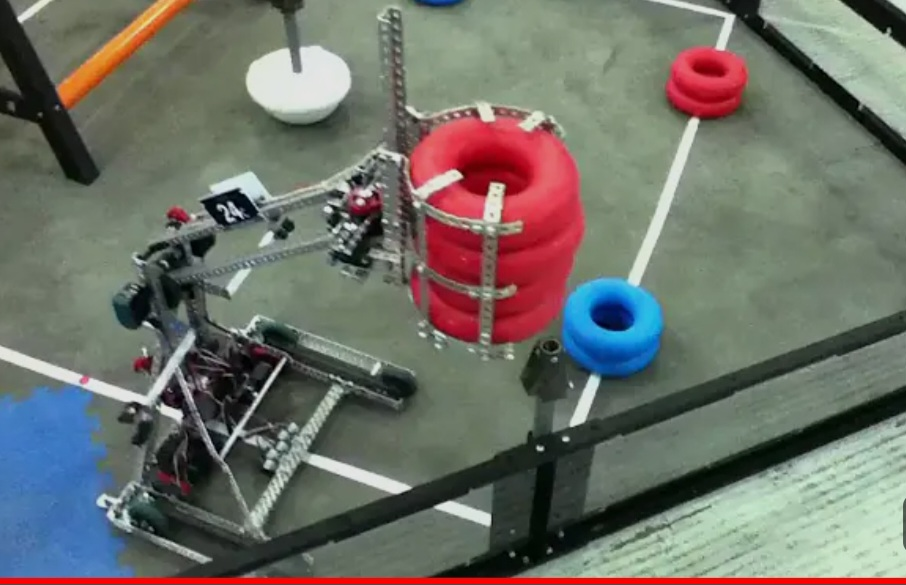
\includegraphics[width=0.5\linewidth]{images/RoundUp.jpeg}
    \caption{Round Up Meta}
    \label{fig:round-up}
\end{figure}
\section*{Design Process}
When designing the bot in fusion, an arc was drawn between the stake and the intake with the center-point of the arc being the location where the pivot would have to be in order to make the arm work. (show a picture of the arc in fusion here) when the pivot was chosen, a c channel was erected to meet the pivot point. From there, gearing and the axle were added along with the 2bar in order to control the length of the pivot of the grabbing mechanism. On the grabbing mechanism itself, a 1:1 ratio was established between the pivot and the central pivoting axle using chains. On the axle itself, lock bars were used to connect the low strength axle to the c channel on the grabbing mechanism rigidly. 
\begin{figure} [h!]
    \centering
    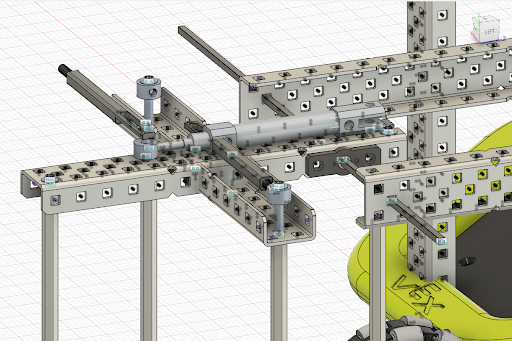
\includegraphics[width=0.5\linewidth]{images/Bot Idea One.png}
    \caption{Mechanism Concept}
    \label{fig:bot-idea-one}
\end{figure} 
\section*{Mechanism Concept}
The concept was that a pneumatic would provide linear force and a separate mechanism would translate the linear force into rotational force which would be able to rotate 90 degrees and force a steel plate under the ring to lock it into place. The only issue: there is not a good space efficient way to translate the force using standard vex parts. The best solution to this problem seemed to be to machine a custom part out of vex parts to accomplish the given task. A part was drawn that would have a slot for the force to be translated in (pinslot mech), and a threaded end on the opposite end of the bar which connected to a shaft collar on the opposite end of the spacing rod.

\section*{Custom Parts Manufacturing}
The following process would be used to make the custom parts:
\begin{itemize}
\item Part off the high strength axle at length
\item Mill the slot on the x axis in order to create the bypass slot on the part
\item Mill the slot on the z axis for the pin screw to sit in
\item Turn down the other side of the part to dimension in order to create a cylinder
\item Cut threads into the turned down cylinder with a die
\item Gently file the part to remove sharp edges
\end{itemize}
 \begin{figure}[h!]
     \centering
     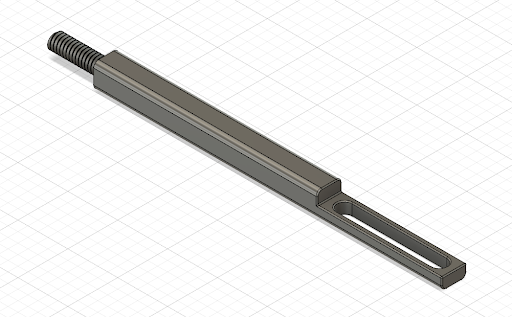
\includegraphics[width=0.5\linewidth]{images/Milled Part.png}
     \caption{Milled Part}
     \label{fig:milled-part}
 \end{figure}
\section*{Design Abandonment}
After drawings were finished, a critical flaw was exposed in the concept: the rings will not be able to bypass the 2bar supports with the constant downward position of the grabbing mechanism. Thus, the design was abandoned with no reasonable solutions to the problem.
\white{Second Bot Idea (May 22, 2024)}
\label{Second-Bot-Idea}
\chapterauthor{Ian Smith}
\info{Ian Smith}{Second Bot Idea}{May 22, 2024}
\section*{Second Robot Idea}

After the failure of the first robot idea, it was determined in a team meeting that the best course of action going forward would be to do the other original idea: an over-engineered clawbot. This concept would be somewhat similar to that last one with a specified pickup area, a stake on a Mogo mechanism, and a claw mechanism that was capable of picking up two rings at the same time  also, this mechanism would be capable of descoring off of the rings, which the last design would not be able to proficiently do.

\section*{Design Considerations}

When going about this idea, {Chase originally came up with the idea of using a pneumatic wrist in order to change position, but it was quickly determined that the binary positions of such a wrist would not provide much benefit. It was then determined that a locked position would be needed on the end of the two bar radius link, and due to motor constraints, the claw would have to be activated pneumatically.
\begin{figure}[h]
    \centering
    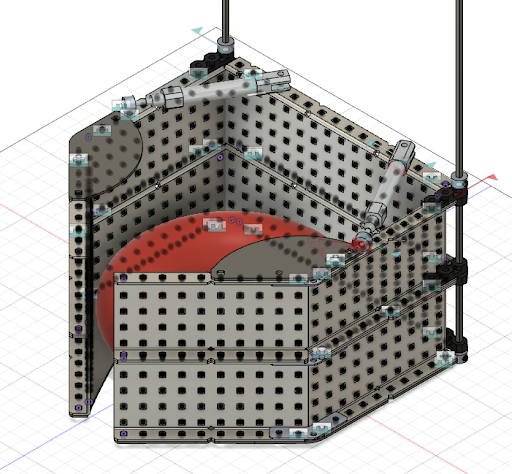
\includegraphics[width=0.5\linewidth]{images/Bot Idea Two.png}
    \caption{Caption}
    \label{fig:bot-idea-two}
\end{figure}
\pagebreak
\section*{CAD Design}
After a general concept was drawn up at practice, I went home and started drawing up some CAD for the idea. When making the CAD, the general idea was to try to use mostly VEX parts for prototyping cases and not use too much laser cut poly-carbonate in the initial design. After carefully considering ring size and the like, it was decided to stack two 10 x 5 aluminum C channels with the 45 degree gusset part. When the jaws were done, the back-plate and pivot for the jaws were built. From there the pneumatics were drawn with a basic motion inspired by wings from over under were used. The last step of the claw was to find a way to hold rings. While it could have been done with steel 1x plating, after consideration it was determined to make the parts out of laser cut poly-carbonate. The parts were drawn up to follow the pattern of the jaws with traditional VEX shapes for aesthetic reasons.

\section*{Design Challenges}

When the idea was about to be conceptualized on the drivetrain, a key flaw was exposed: the bot would not be able to score on the wall stakes. One solution was drawn up to fix this, a pneumatic wrist similar to Chase's original idea, but that was quickly thrown out due to the benefits of a different bot design.

\section*{New Bot Design}

The new bot design was going to be similar to many other robots seen on the internet at the time, but with a 2 bar raisable intake. This design was drawn up by  Connor and heavily inspired by 78A.
 %May 22
\identify{Identify the Challenge \& Set Goals: Drivetrain (May 23, 2024)}
\label{Identify-the-Challenge-&-Set-Goals:-Drivetrain}
\chapterauthor{Caleb Bachmeier}
\info{Caleb Bachmeier}{Identify the Challenge \& Set Goals: Drivetrain}{May 23, 2024}
\textbf{Goal}: We Will identify an objective for our robot so that we can address it and build an effective drivetrain.
\section*{Problem Statement}
We must create a mechanism that effectively moves around the field and provides mounting opportunities for additional mechanisms.
\section*{Solution Requirements}
\begin{itemize}
    \item Must only use legal VEX VRC parts
    \item Must fit in the 18" x 18" x 18" cube
    \item Must use no more than 88 watts (eight, eleven watt motors). 
    \item Another, often overlooked, problem is the scarcity of parts, parts are not unlimited. One of these parts is 48 tooth gears, of which we only have six. 
\end{itemize}
\begin{itemize}
    \item Minimum speed of 65 inches/second. From teams we have analyzed such as our sister teams \textit{"7686A" }\cite{7686a}, \textit{7686B} \cite{7686b}, and \textit{7686C} \cite{7686c}, we believe that this goal is feasible and a good minimum to meet.
    \item We would like to use a maximum of 6, eleven watt motors, so we can use the rest on other components.
    \item Must fit within a length of 15". Although 18" is the maximum starting length, we want some room to add other components later.
\end{itemize}
\brainstorm{Brainstorm \& Diagram (May 25, 2024)}
\label{Brainstorm-&-Diagram}
\chapterauthor{Caleb Bachmeier}
\info{Caleb Bachmeier}{Brainstorm \& Diagram}{May 25, 2024}
\textbf{Goal}: We will brainstorm possible solutions for our drive train so we can choose the best one that meets our solution requirements.
\section*{Possible Solution - Wheel Choice}
\noindent
\textbf{Omni-Directional Wheels}:

\noindent
\textbf{Pros}:
\begin{itemize}
    \item Quick and smooth turning
    \item Allows for a certain unique Omni-Directional driving style
\end{itemize}
\textbf{Cons}:
\begin{itemize}
    \item Little to no side to side traction
\end{itemize}
\textbf{Traction Wheels}

\noindent
\textbf{Pros}:
\begin{itemize}
    \item Excellent grip on soft surfaces (Including foam tiles used on the field)
    \item Allows for a precise more traditional driveing style
\end{itemize}
\textbf{Cons}:
\begin{itemize}
    \item Less maneuverability. Especially in comparison to Omni-Directional Wheels
\end{itemize}
\textbf{Flex Wheels}:

\noindent
\textbf{Pros}:
\begin{itemize}
    \item  Conform to the surface the ride on providing even more grip than traction wheels.
\end{itemize}
\textbf{Cons}:
\begin{itemize}
    \item They are not ideal for drive-trains due the many adapters required.
\end{itemize}

\begin{figure}[hbt!] % Use [hbt!] to place the figures on the same page
    \begin{minipage}{.5\textwidth}
        \centering
        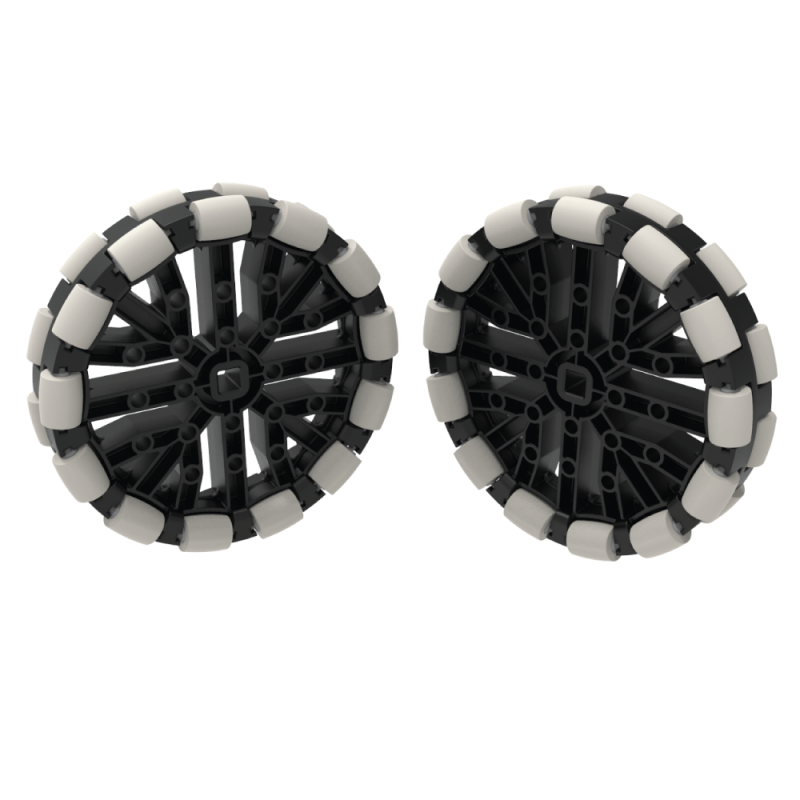
\includegraphics[width=.8\linewidth]{images/Omni Wheels.jpg}
        \caption{Omni-Directional Wheels}
        \label{fig:omni-directional-wheels}
    \end{minipage}%
    \begin{minipage}{.5\textwidth}
        \centering
        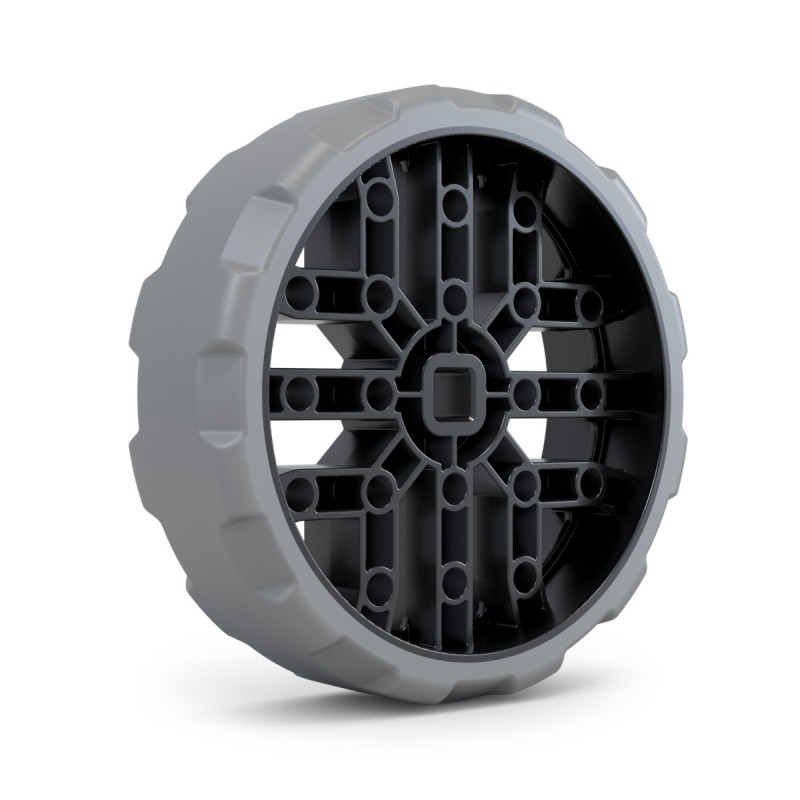
\includegraphics[width=.8\linewidth]{images/Traction Wheels.jpg}
        \caption{Traction Wheels}
        \label{fig:traction-wheels}
    \end{minipage}
    \begin{minipage}{.5\textwidth}
        \centering
        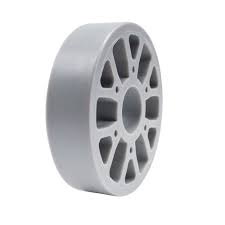
\includegraphics[width=.8\linewidth]{images/Flex Wheels.jpg}
        \caption{Flex Wheels}
        \label{fig:flex-wheels}
    \end{minipage}%
\end{figure}
\pagebreak
\section*{Possible Solution - Cartridge Type}
\noindent 
\textbf{Red Cartridge}

- Spins up to 100 RPM

- Usually used for mechanisms requiring extra torque -- traditionally not a good choice for a drivetrain

\noindent
\textbf{Pros}:
\begin{itemize}
    \item Very strong
    \item Great Acceleration
\end{itemize}
\textbf{Cons}:
\begin{itemize}
    \item Very slow 
    \item Loses torque due to increased friction in the cartridge (36:1 planetary ratio)
\end{itemize}

\noindent 
\textbf{Green Cartridge}

- Spins up to 200 RPM

- Usually used for mechanisms that require a balance between strength and speed -- common because of a shared ratio between 5.5 watt motor

\noindent
\textbf{Pros}:
\begin{itemize}
    \item Has a good balance between speed and torque 
    \item Versitile, easy to gear speed; compatable with 5.5 watt motors
\end{itemize}
\textbf{Cons}:
\begin{itemize}
    \item Often too slow for most drivetrains and lacking enough torque for most mechanisms
\end{itemize}

\textbf{Blue Cartridges}

- Spins up to 600 RPM

- Usually used for mechanisms requiring extra speed such as flywheels

\noindent
\textbf{Pros}:
\begin{itemize}
    \item Very Fast
    \item Causes minimal friction due to the 6:1 planetary ratio
\end{itemize}
\textbf{Cons}:
\begin{itemize}
    \item Significantly lacks torque
\end{itemize}

\begin{figure}[hbt] % Use [hbt!] to place the figures on the same page
    \begin{minipage}{.5\textwidth}
        \centering
        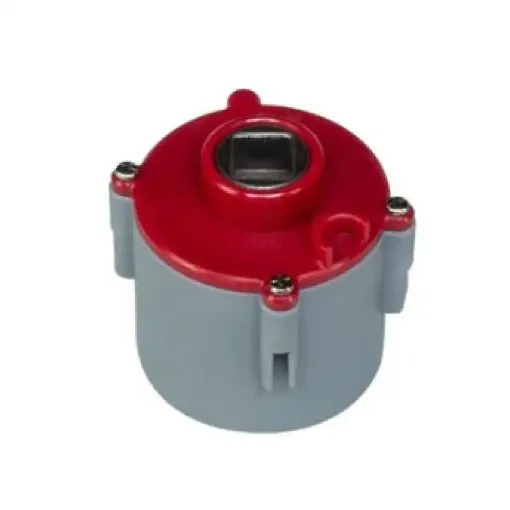
\includegraphics[width=.8\linewidth]{images/Red-Cartridge.png}
        \caption{Red Cartridge}
        \label{fig:red-cartridge}
    \end{minipage}%
    \begin{minipage}{.5\textwidth}
        \centering
        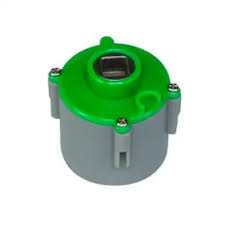
\includegraphics[width=.8\linewidth]{images/Green Cartridge.jpg}
        \caption{Green Cartridge}
        \label{fig:green-cartridge}
    \end{minipage}
    \begin{minipage}{.5\textwidth}
        \centering
        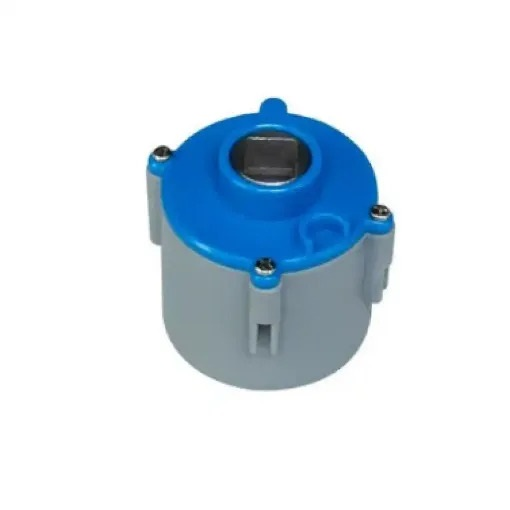
\includegraphics[width=.8\linewidth]{images/Blue-Cartridge.jpg}
        \caption{Blue Cartridge}
        \label{fig:blue-cartridge}
    \end{minipage}%
\end{figure}

% Add in the picture of the motor curve chart here %

% https://kb.vex.com/hc/en-us/articles/360044325872-Understanding-V5-Smart-Motor-11W-Performance %

\pagebreak
\section*{Possible Solution - Drive Type}

\blueref{fig:standard-omnidirectional-wheels}{\textbf{Standard Omnidirectional Wheels -}} 

- Omnidirectional Wheels set up in a tank drive orientation 

- Most common drivetrain type

\noindent
\textbf{Pros}:
\begin{itemize}
    \item Fast
    \item Simple
    \item Compact 
\end{itemize}
\textbf{Cons}:
\begin{itemize}
    \item Roller mechanisms greatly reduce traction due to material type
    \item Moves in only two directions 
\end{itemize}

\blueref{fig:mecanum}{Mecanum Wheels} 

- Specialized wheel design to allow movement in all directions

- Mecanum Wheels set up in a tank drive orientation 

- Second most popular drive design 
\noindent
\textbf{Pros}:
\begin{itemize}
    \item Moves in all directions
    \item Has the power of all motors in all directions
\end{itemize}
\textbf{Cons}:
\begin{itemize}

    \item Bulky
    \item Can be difficult to code
\end{itemize}

\blueref{fig:hexagonal}{\textbf{Holonomic / X-Drive -}} 

- Omnidirectional Wheels set up in a hexagonal orientation

- Two sets of parallel lines with each wheel oriented 45 degrees from a standard tanks drive 

- Third most common drive-train type 

\noindent
\textbf{Pros}:
\begin{itemize}
    \item Moves in all directions
    \item Less bulky than Mecanum drive 
    \item Has the power of all motors in all directions
\end{itemize}
\textbf{Cons}:
\begin{itemize}
    \item Complex Programming 
    \item Still comparatively large 
    \item Half as fast in all directions
\end{itemize}

\blueref{fig:h-drive}{\textbf{H-Drive -}} 

- Five omnidirectional wheels set up to look like the letter "H"

- Four wheels set up in a tank drive orientation 

- The fifth wheel is perpendicular to the orientation of the others and moves the drive side to side
\noindent
\textbf{Pros}:
\begin{itemize}
    \item Moves in all directions
    \item Simple
    \item Moves fast in all directions
\end{itemize}
\textbf{Cons}:
\begin{itemize}
    \item Complex programming
    \item Only has the power of 1 motor when moving side to side 
    \item Requires all wheels to be omnidirectional
\end{itemize}

\blueref{fig:traction-wheel-drive}{\textbf{All Traction Wheel Drive -}} 

- Wheel design for more traction

- Traction wheels set up in a tank drive orientation 

\noindent
\textbf{Pros}:
\begin{itemize}
    \item  Excellent traction
    \item Simple
    \item Compact 
\end{itemize}
\textbf{Cons}:
\begin{itemize}

    \item Slow turning
\end{itemize}

\blueref{fig:omnidirectional-and-traction-wheels}{\textbf{Omnidirectinal and Traction Wheels -}} 

- Omnidirectional wheels and Traction wheels set up in a tank drive orientation 

- One or two traction wheels in the middle and omni wheels to the front and rear of it 

\noindent
\textbf{Pros}:
\begin{itemize}
    \item Good traction
    \item Simple
    \item Compact 
\end{itemize}
\textbf{Cons}:
\begin{itemize}
    \item Doens't allow for Omnidirectional driving styles
\end{itemize}

\blueref{fig:tank-treads}{\textbf{Tank Tread -}} 

- Sprockets connected by tread in the VEX
tank tread kit

- Sprockets are oriented in a trIangle that is parallel
to the ground

\noindent
\textbf{Pros}:
\begin{itemize}
    \item Great traction
    \item Strong pushing force
    \item Great at climbing over objects 
\end{itemize}
\textbf{Cons}:
\begin{itemize}
    \item Very slow
    \item Very slow turning 
    \item Tracks can fall apart leaving the robot immobile
\end{itemize}

\blueref{fig:walking-robot}{\textbf{Walking Robot -}} 
- C-Channels that move back and forth

- Looks like a person walking

\noindent
\textbf{Pros}:
\begin{itemize} 
    \item Unique 
    \item Moves over rough terrain
\end{itemize}
\textbf{Cons}:
\begin{itemize}
    \item Very tall
    \item Extremely slow
    \item Does not turn
    \item Looks clunky
\end{itemize}
\begin{center}
    \textbf{Hand drawn images of all Drive Types on following page}
\end{center}
\pagebreak
\begin{figure}[hbt!] % Use [hbt!] to place the figures on the same page
    \begin{minipage}{.5\textwidth}
        \centering
        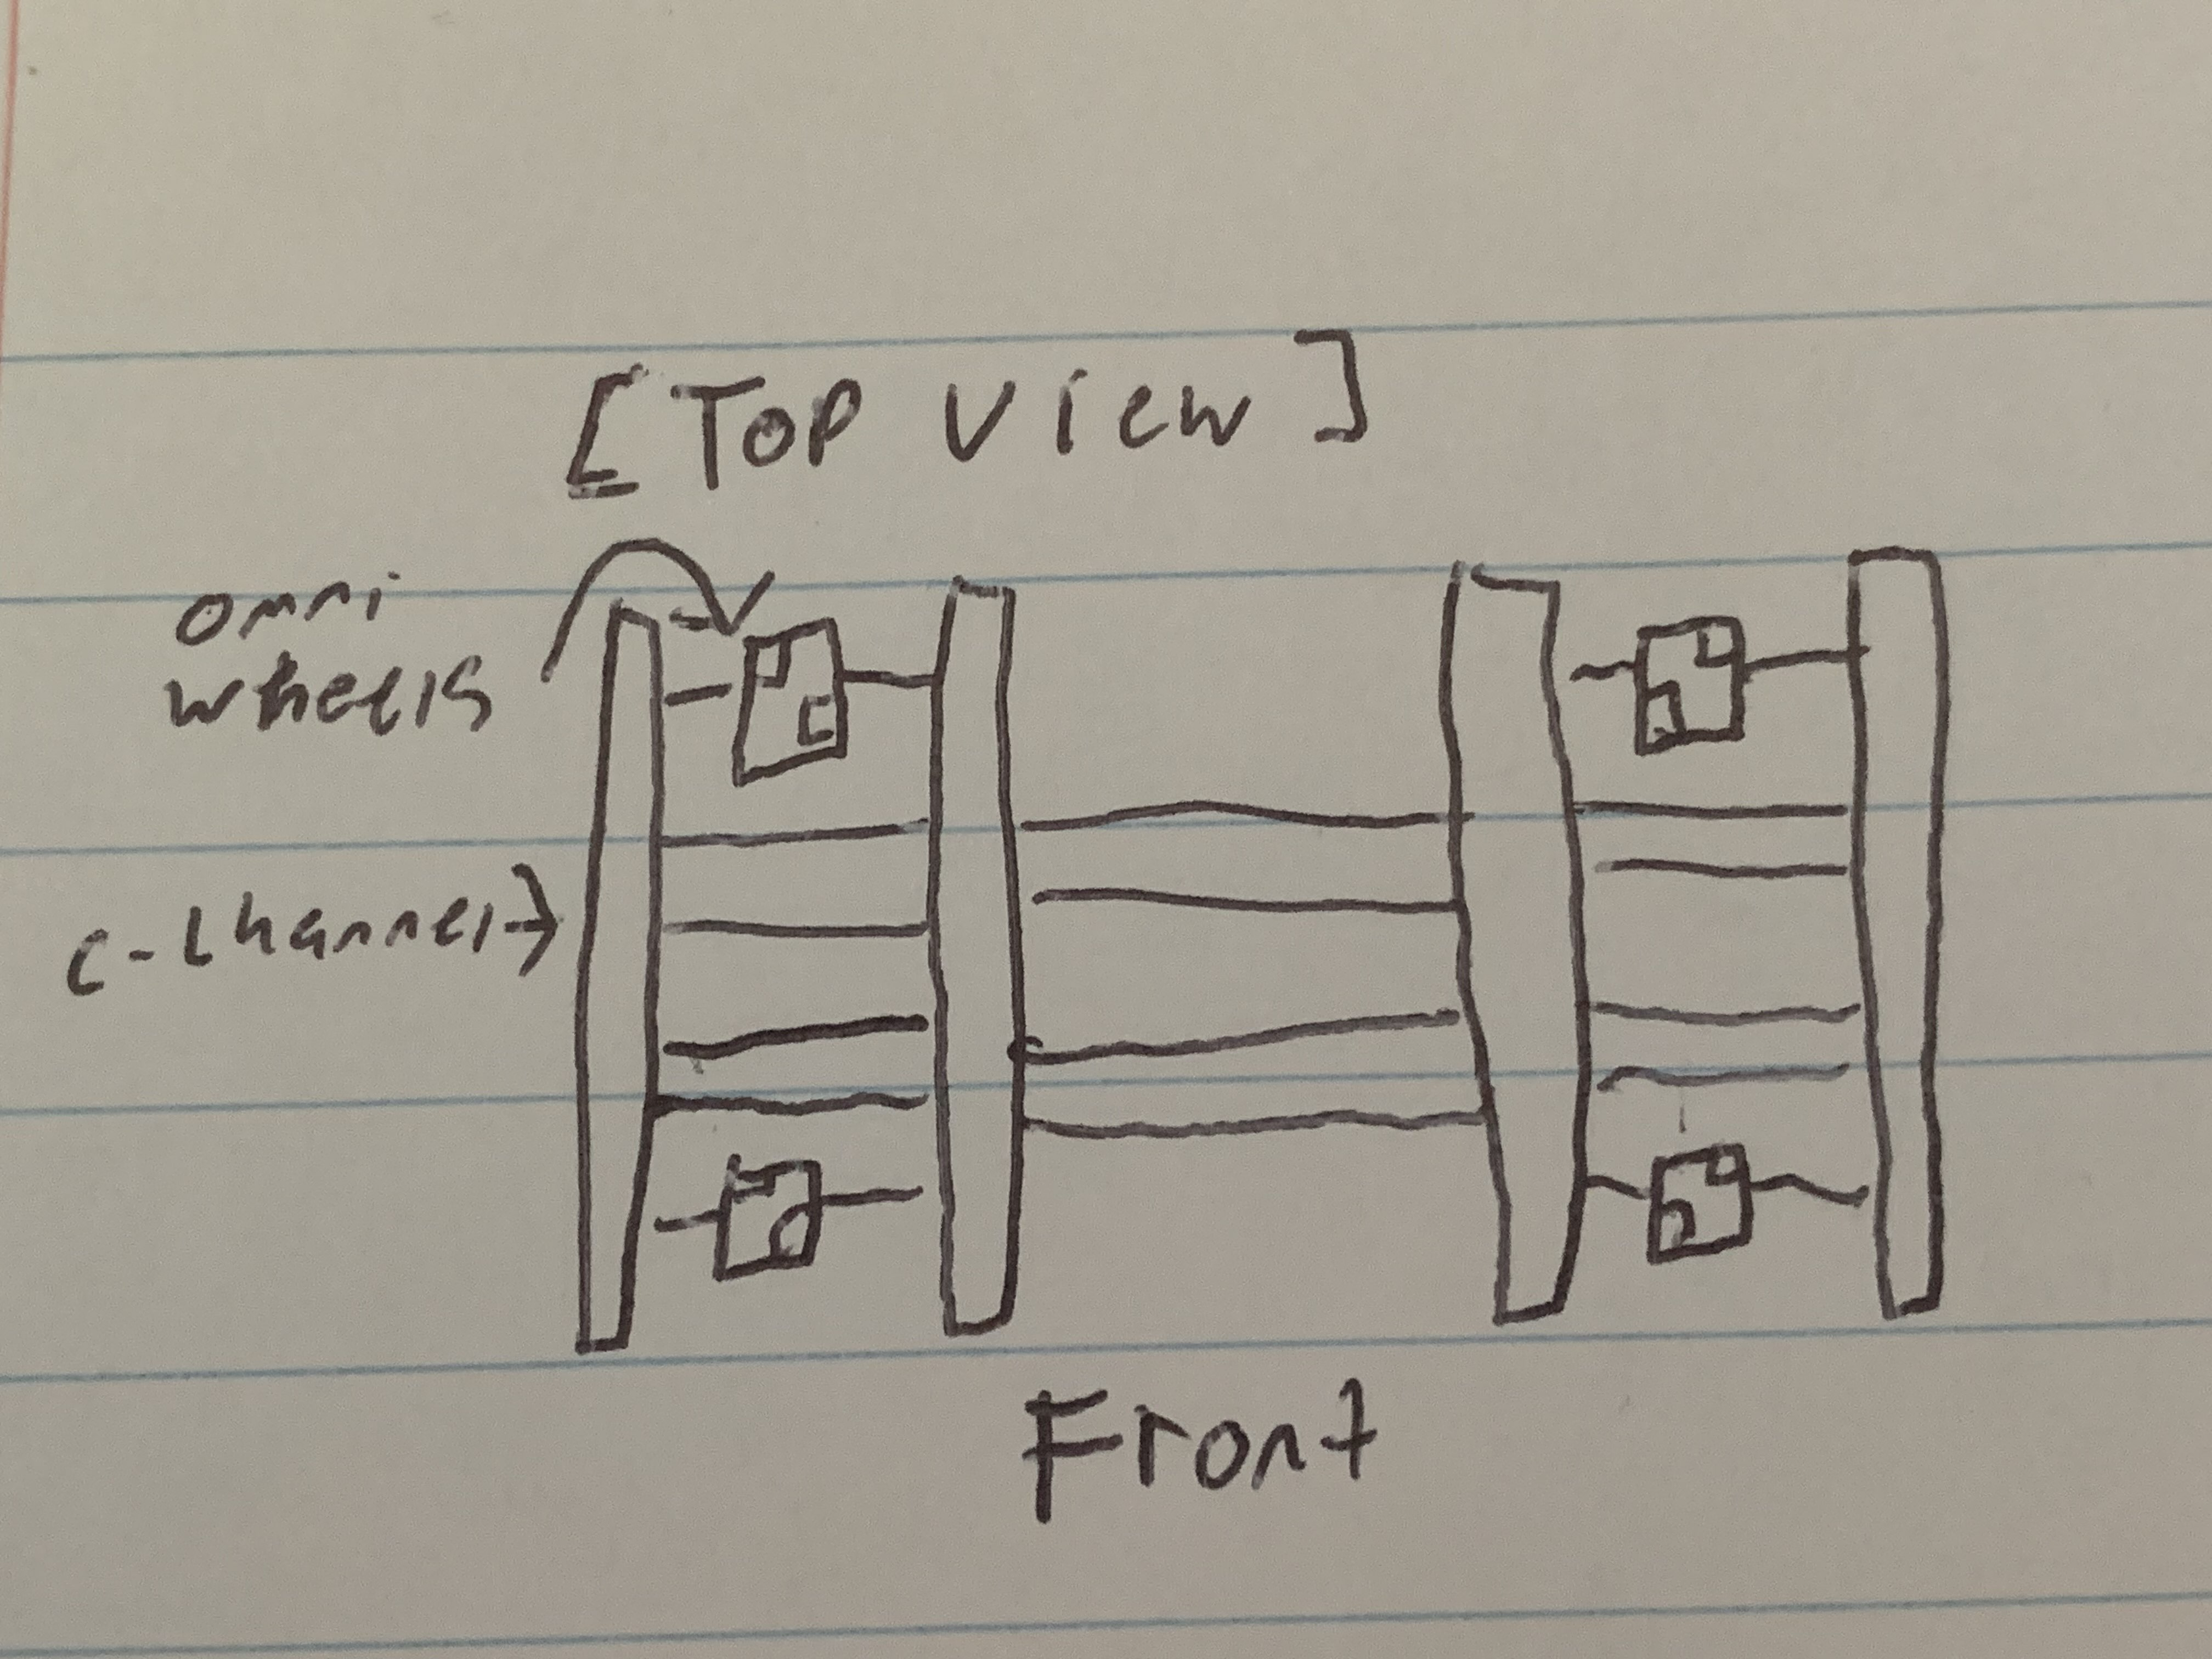
\includegraphics[width=.8\linewidth]{images/Omni Drive.jpg}
        \caption{Standard Omnidirectional} %re draw this with six wheels
        \label{fig:standard-omnidirectional-wheels}
    \end{minipage}%
    \begin{minipage}{.5\textwidth}
        \centering
        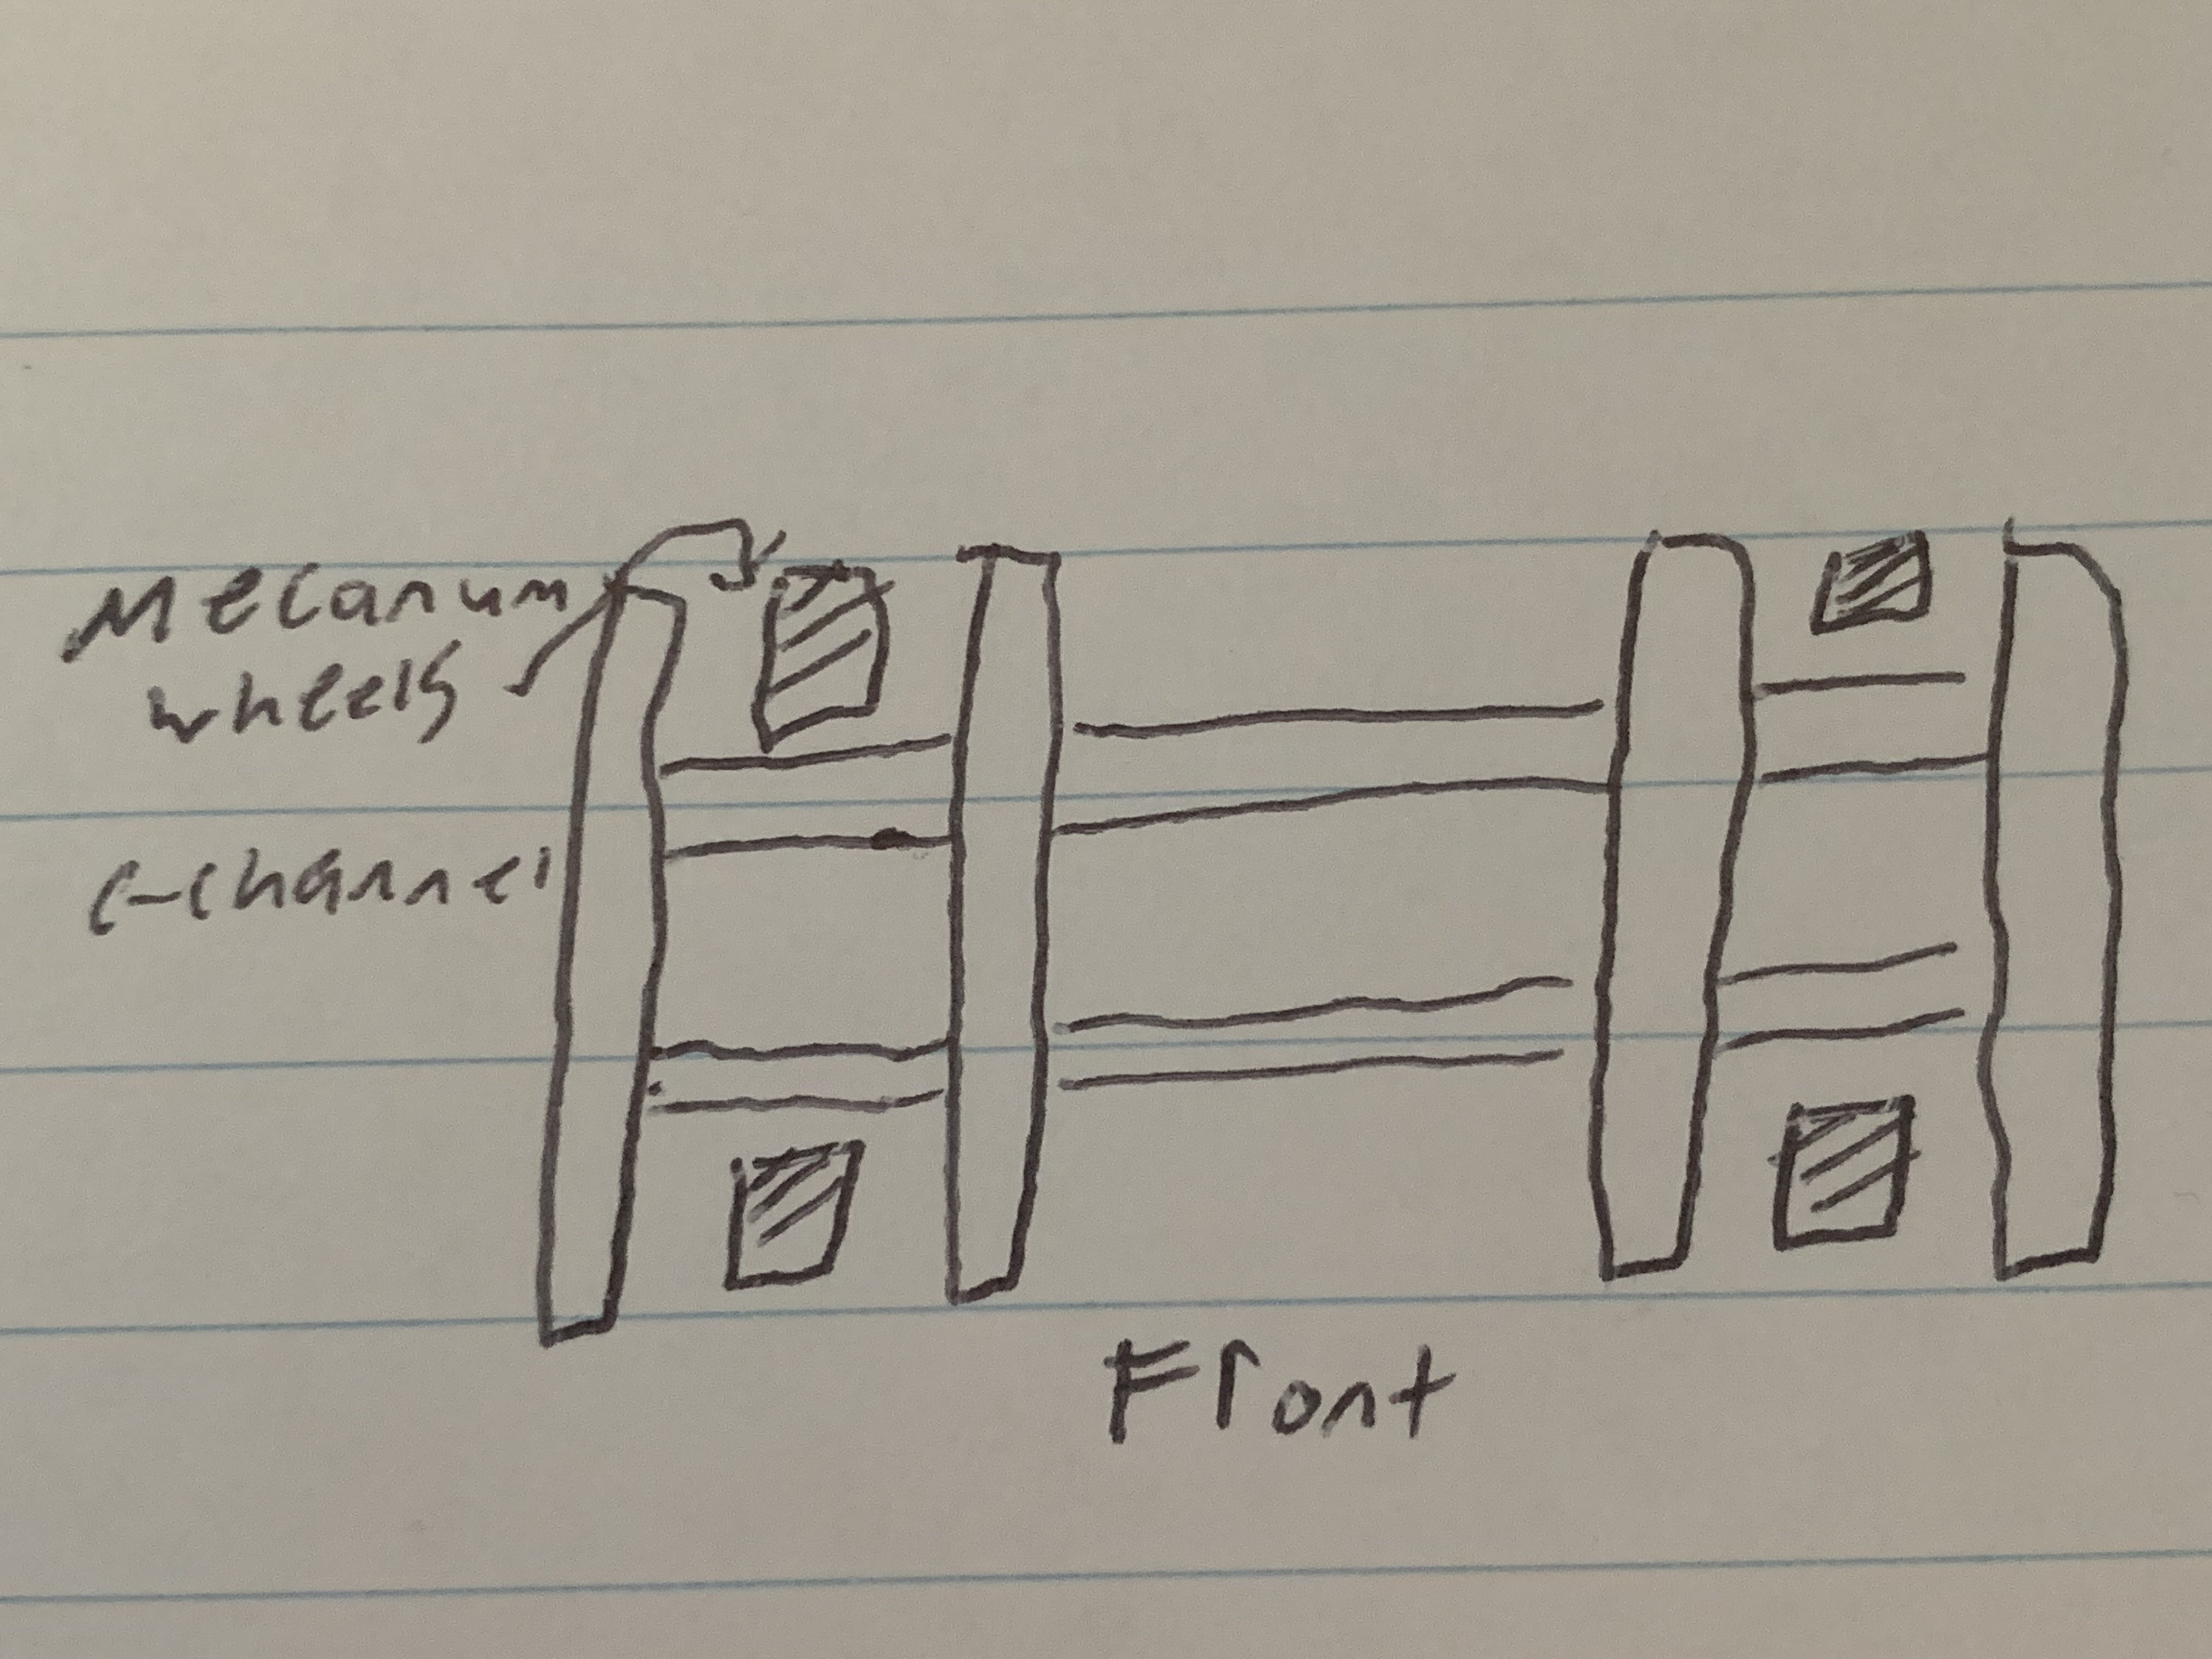
\includegraphics[width=.8\linewidth]{images/Mecanum Drive.jpg}
        \caption{Mecanum}
        \label{fig:mecanum}
    \end{minipage}
    \begin{minipage}{.5\textwidth}
        \centering
        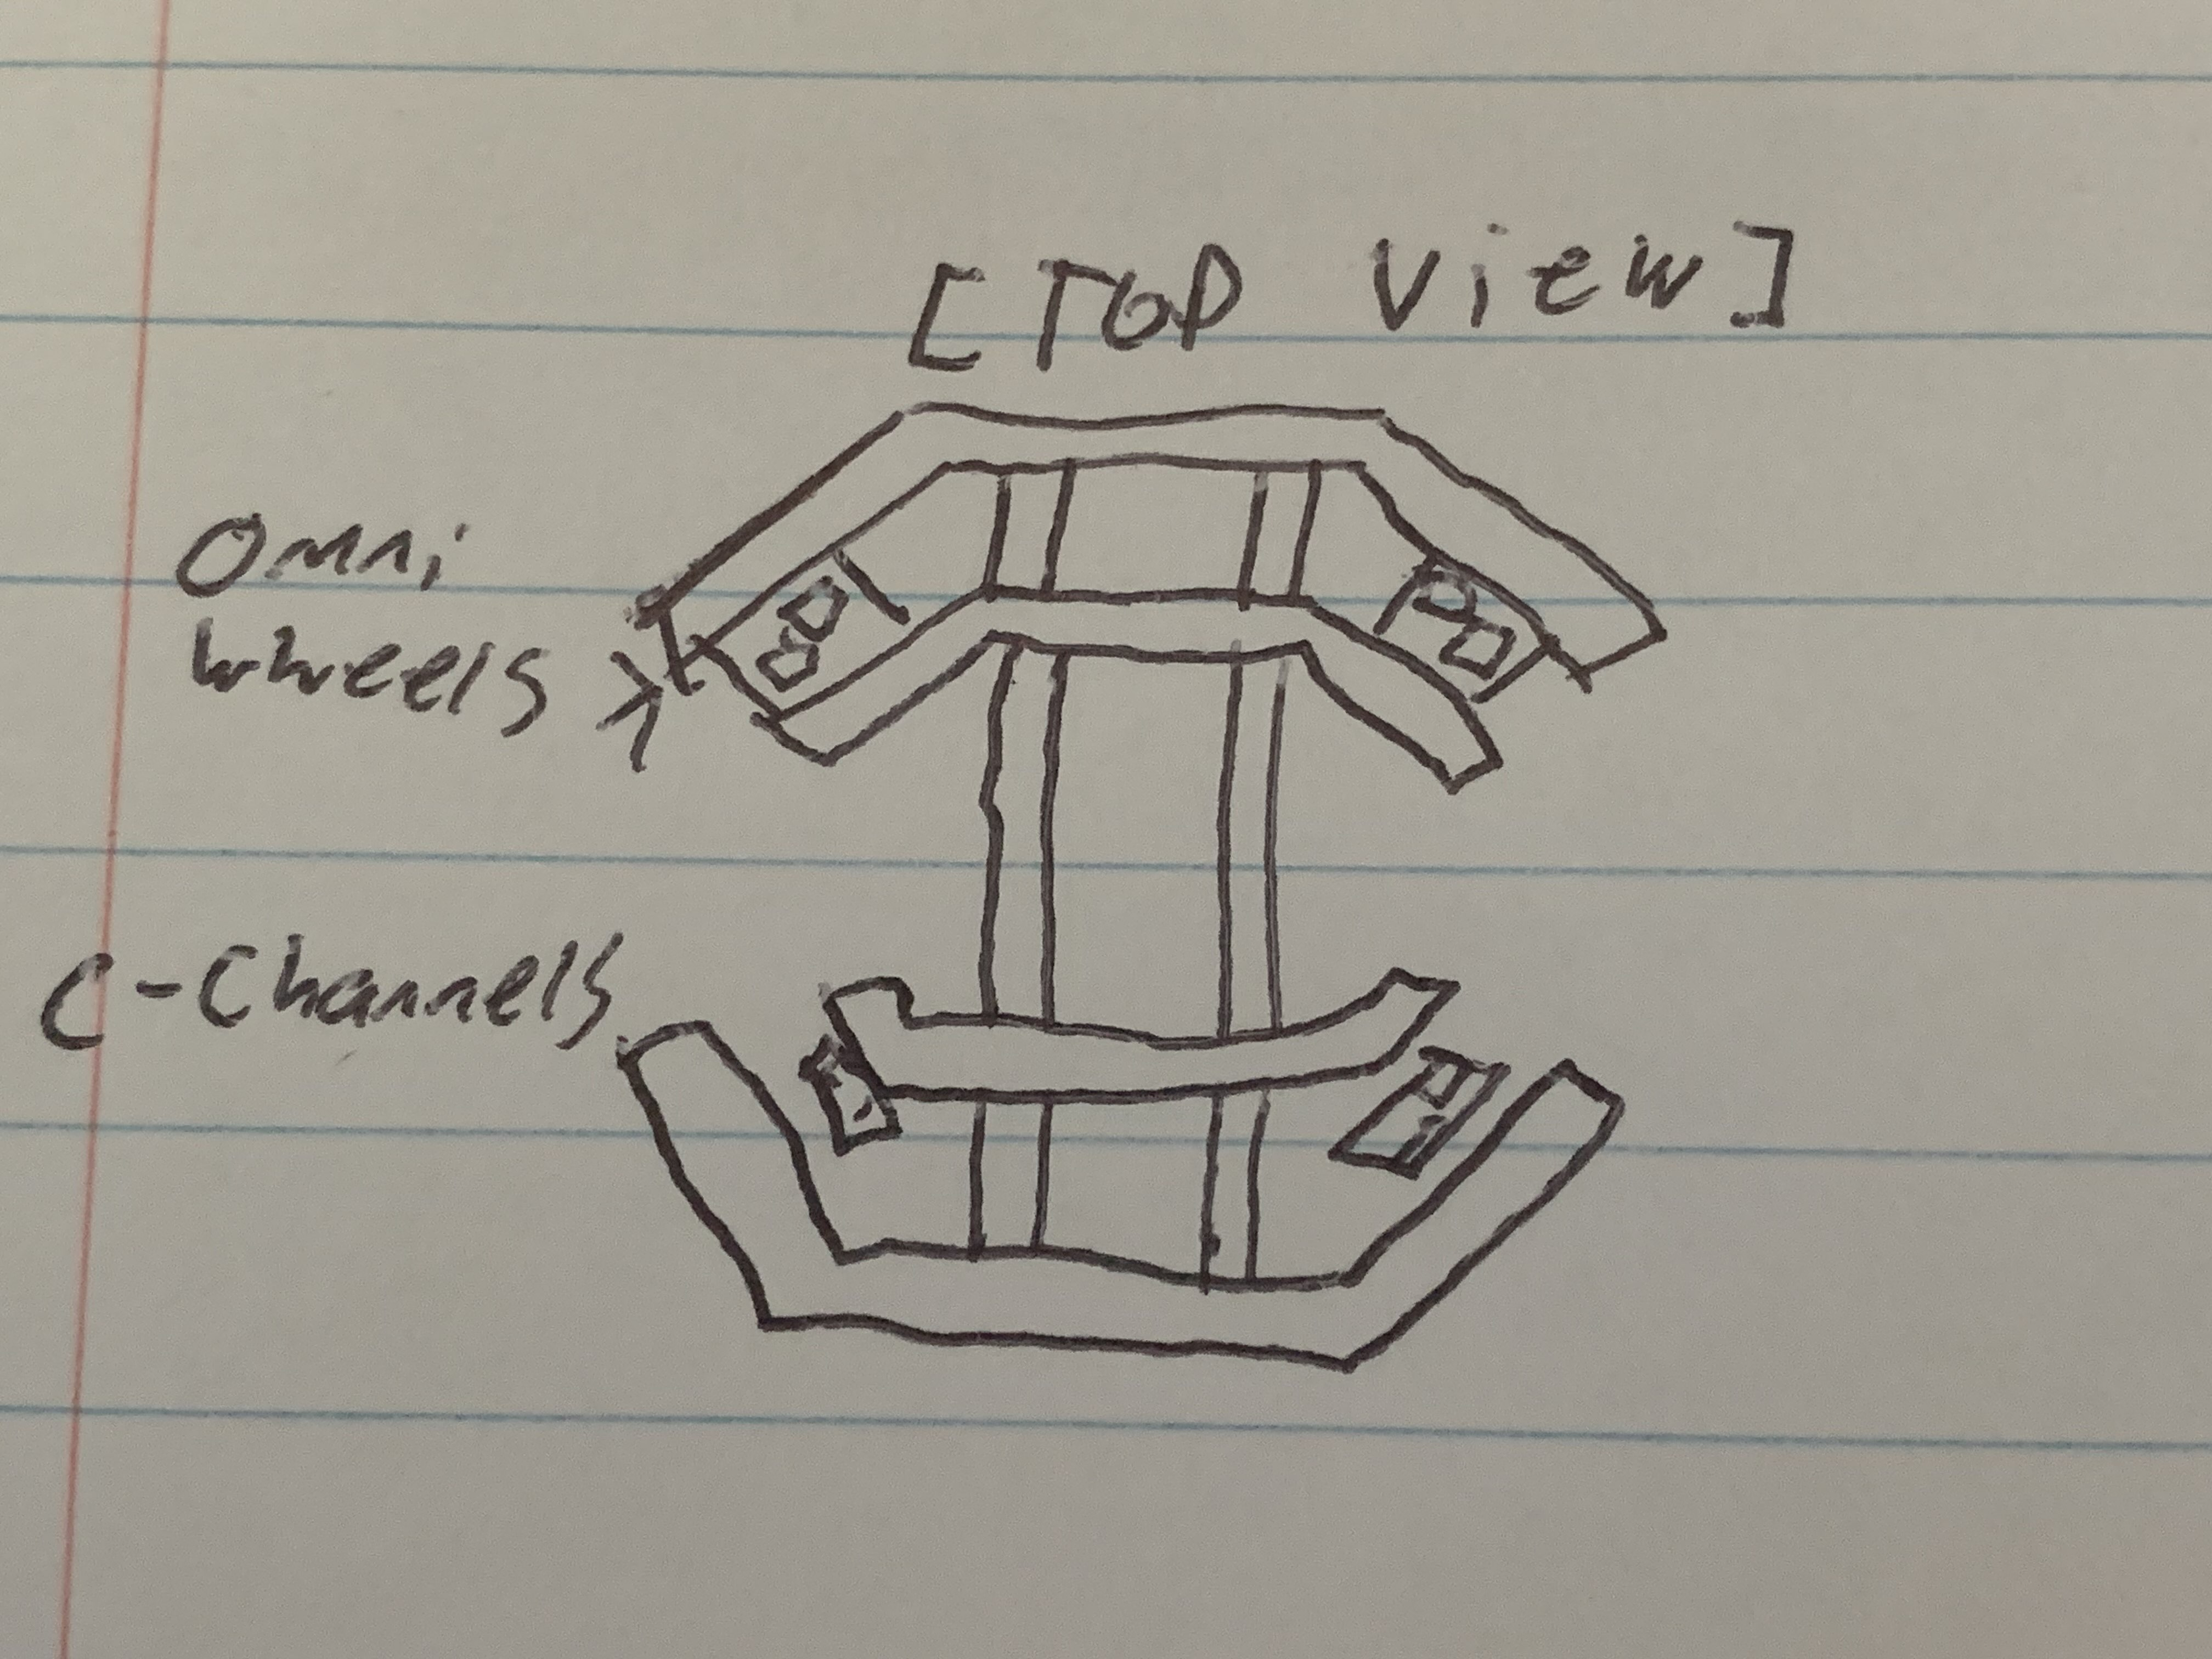
\includegraphics[width=.8\linewidth]{images/Hexagonal Omni Wheels.jpg}
        \caption{Holonomic / X-Drive}
        \label{fig:hexagonal}
    \end{minipage}%
    \begin{minipage}{.5\textwidth}
        \centering
        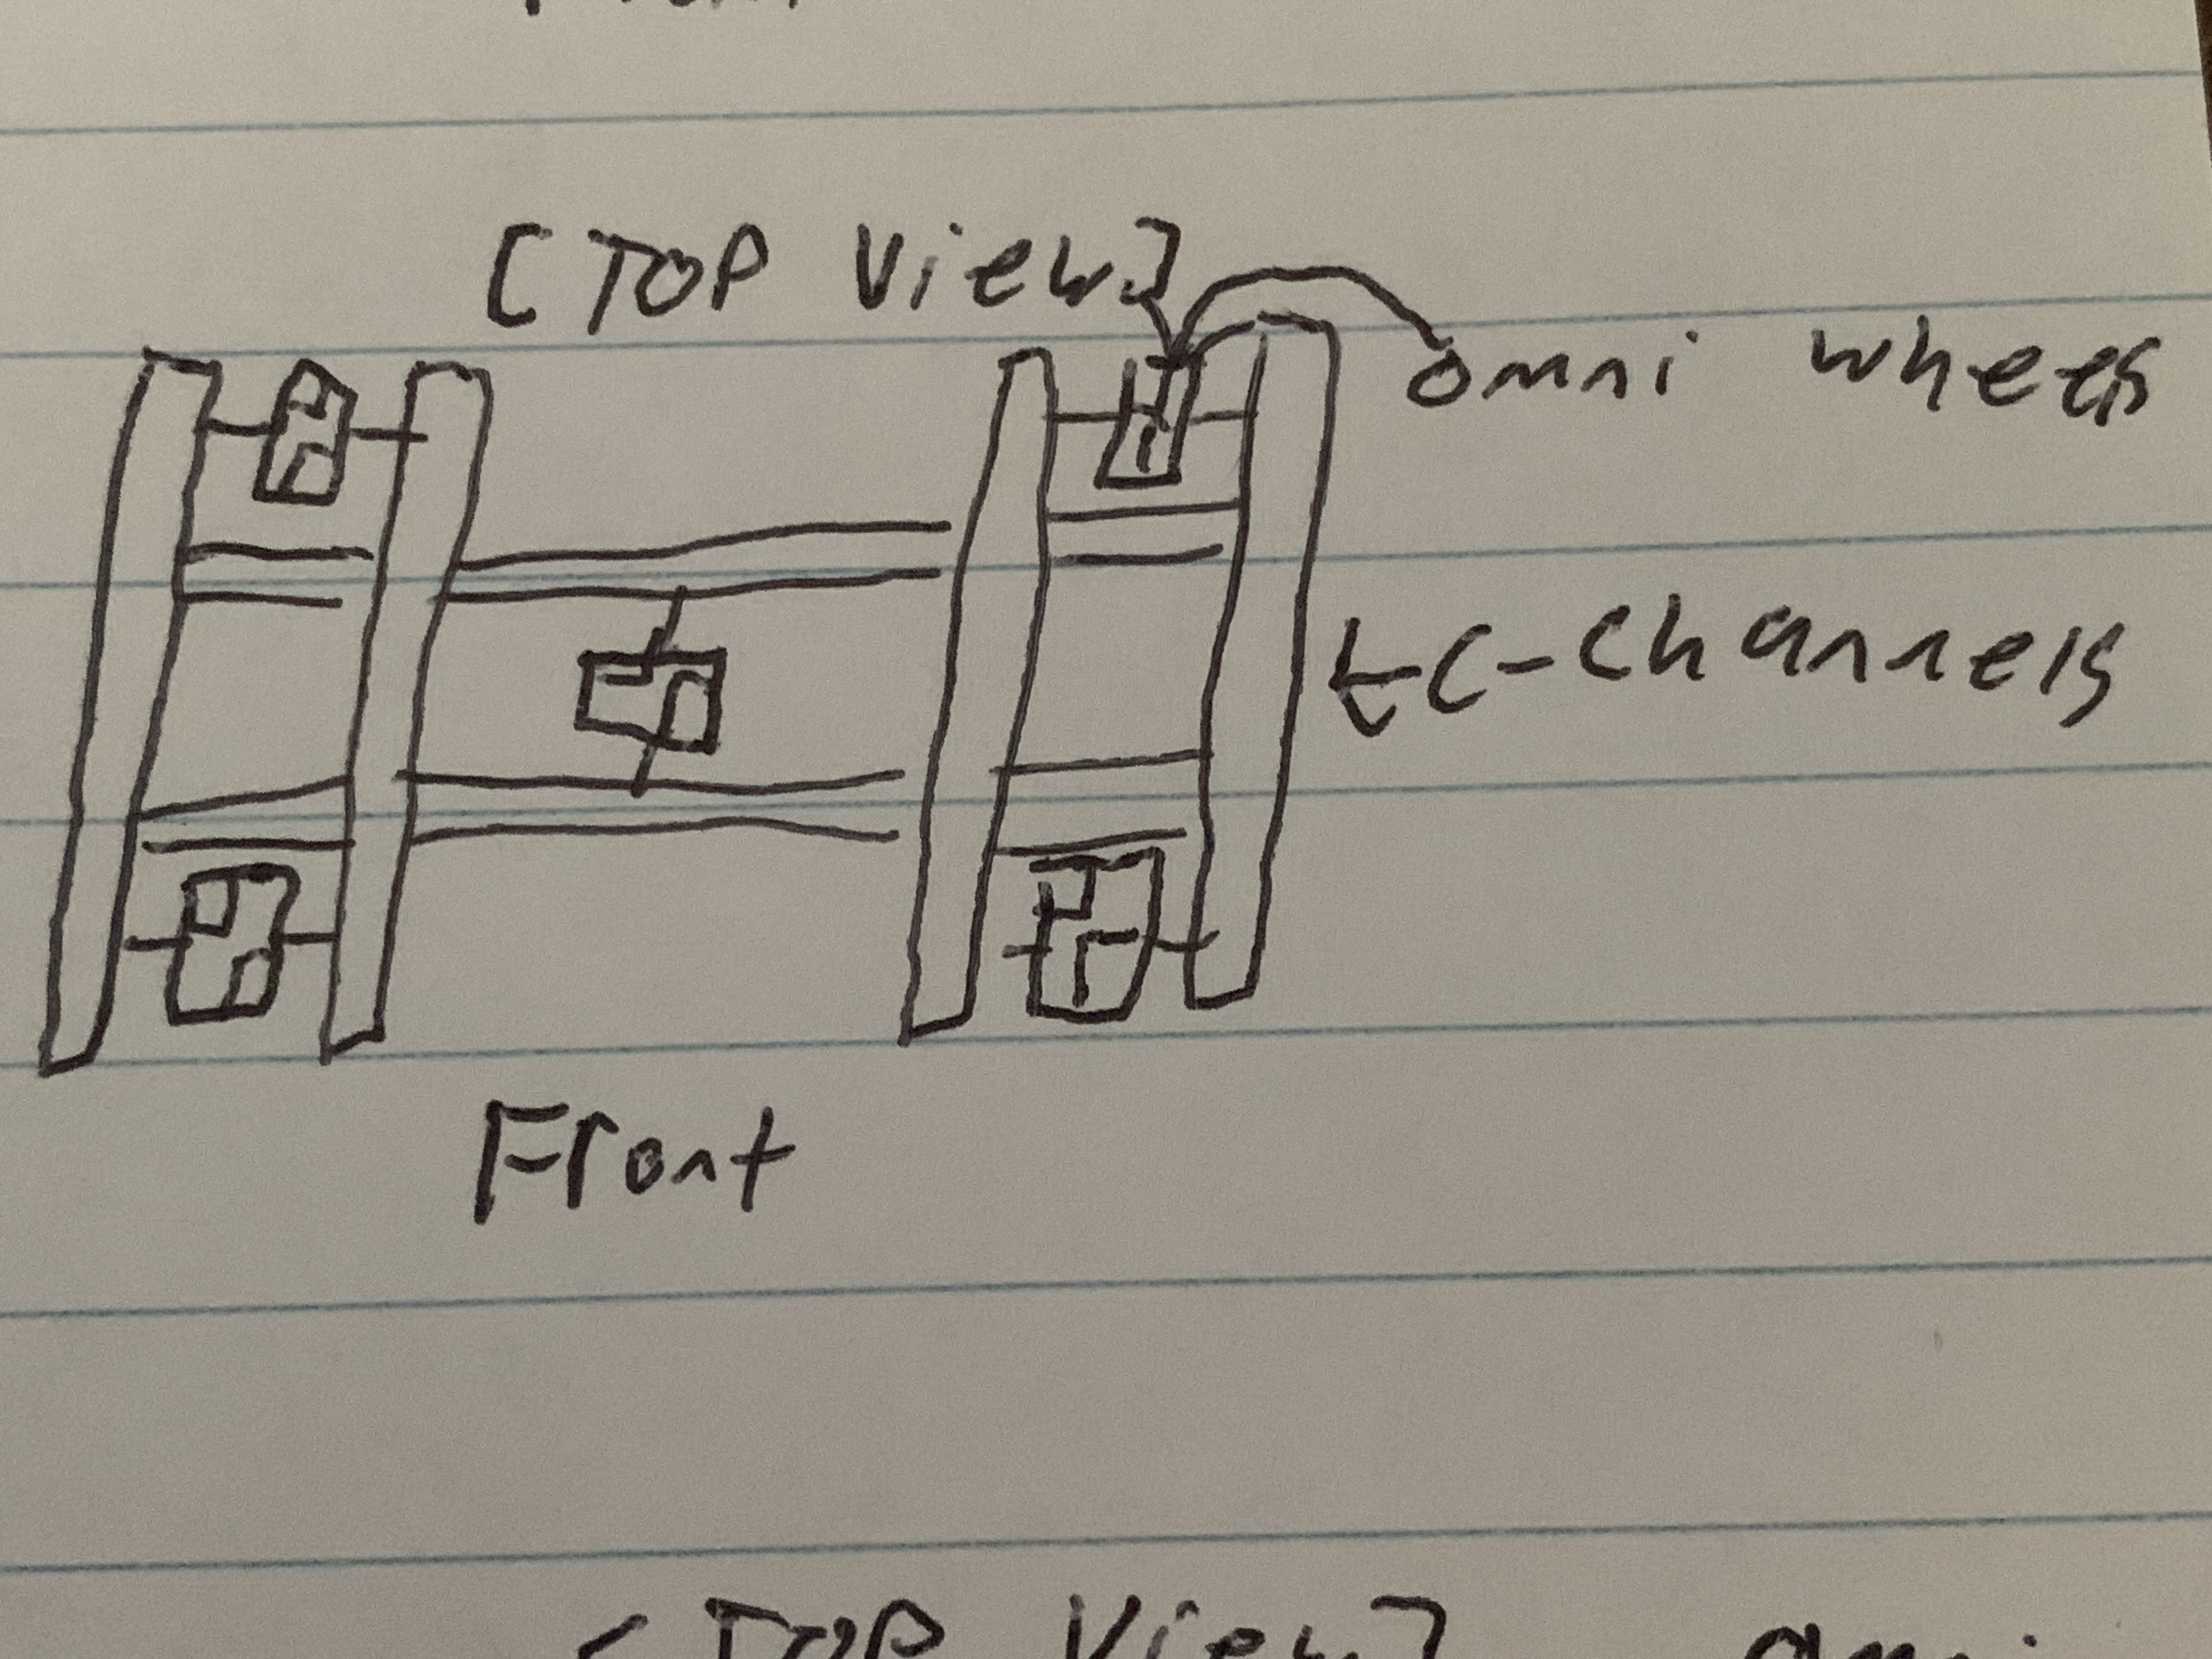
\includegraphics[width=.8\linewidth]{images/5 Omni Wheels.jpg}
        \caption{H-Drive}
        \label{fig:h-drive}
    \end{minipage}
    \begin{minipage}{.5\textwidth}
        \centering
        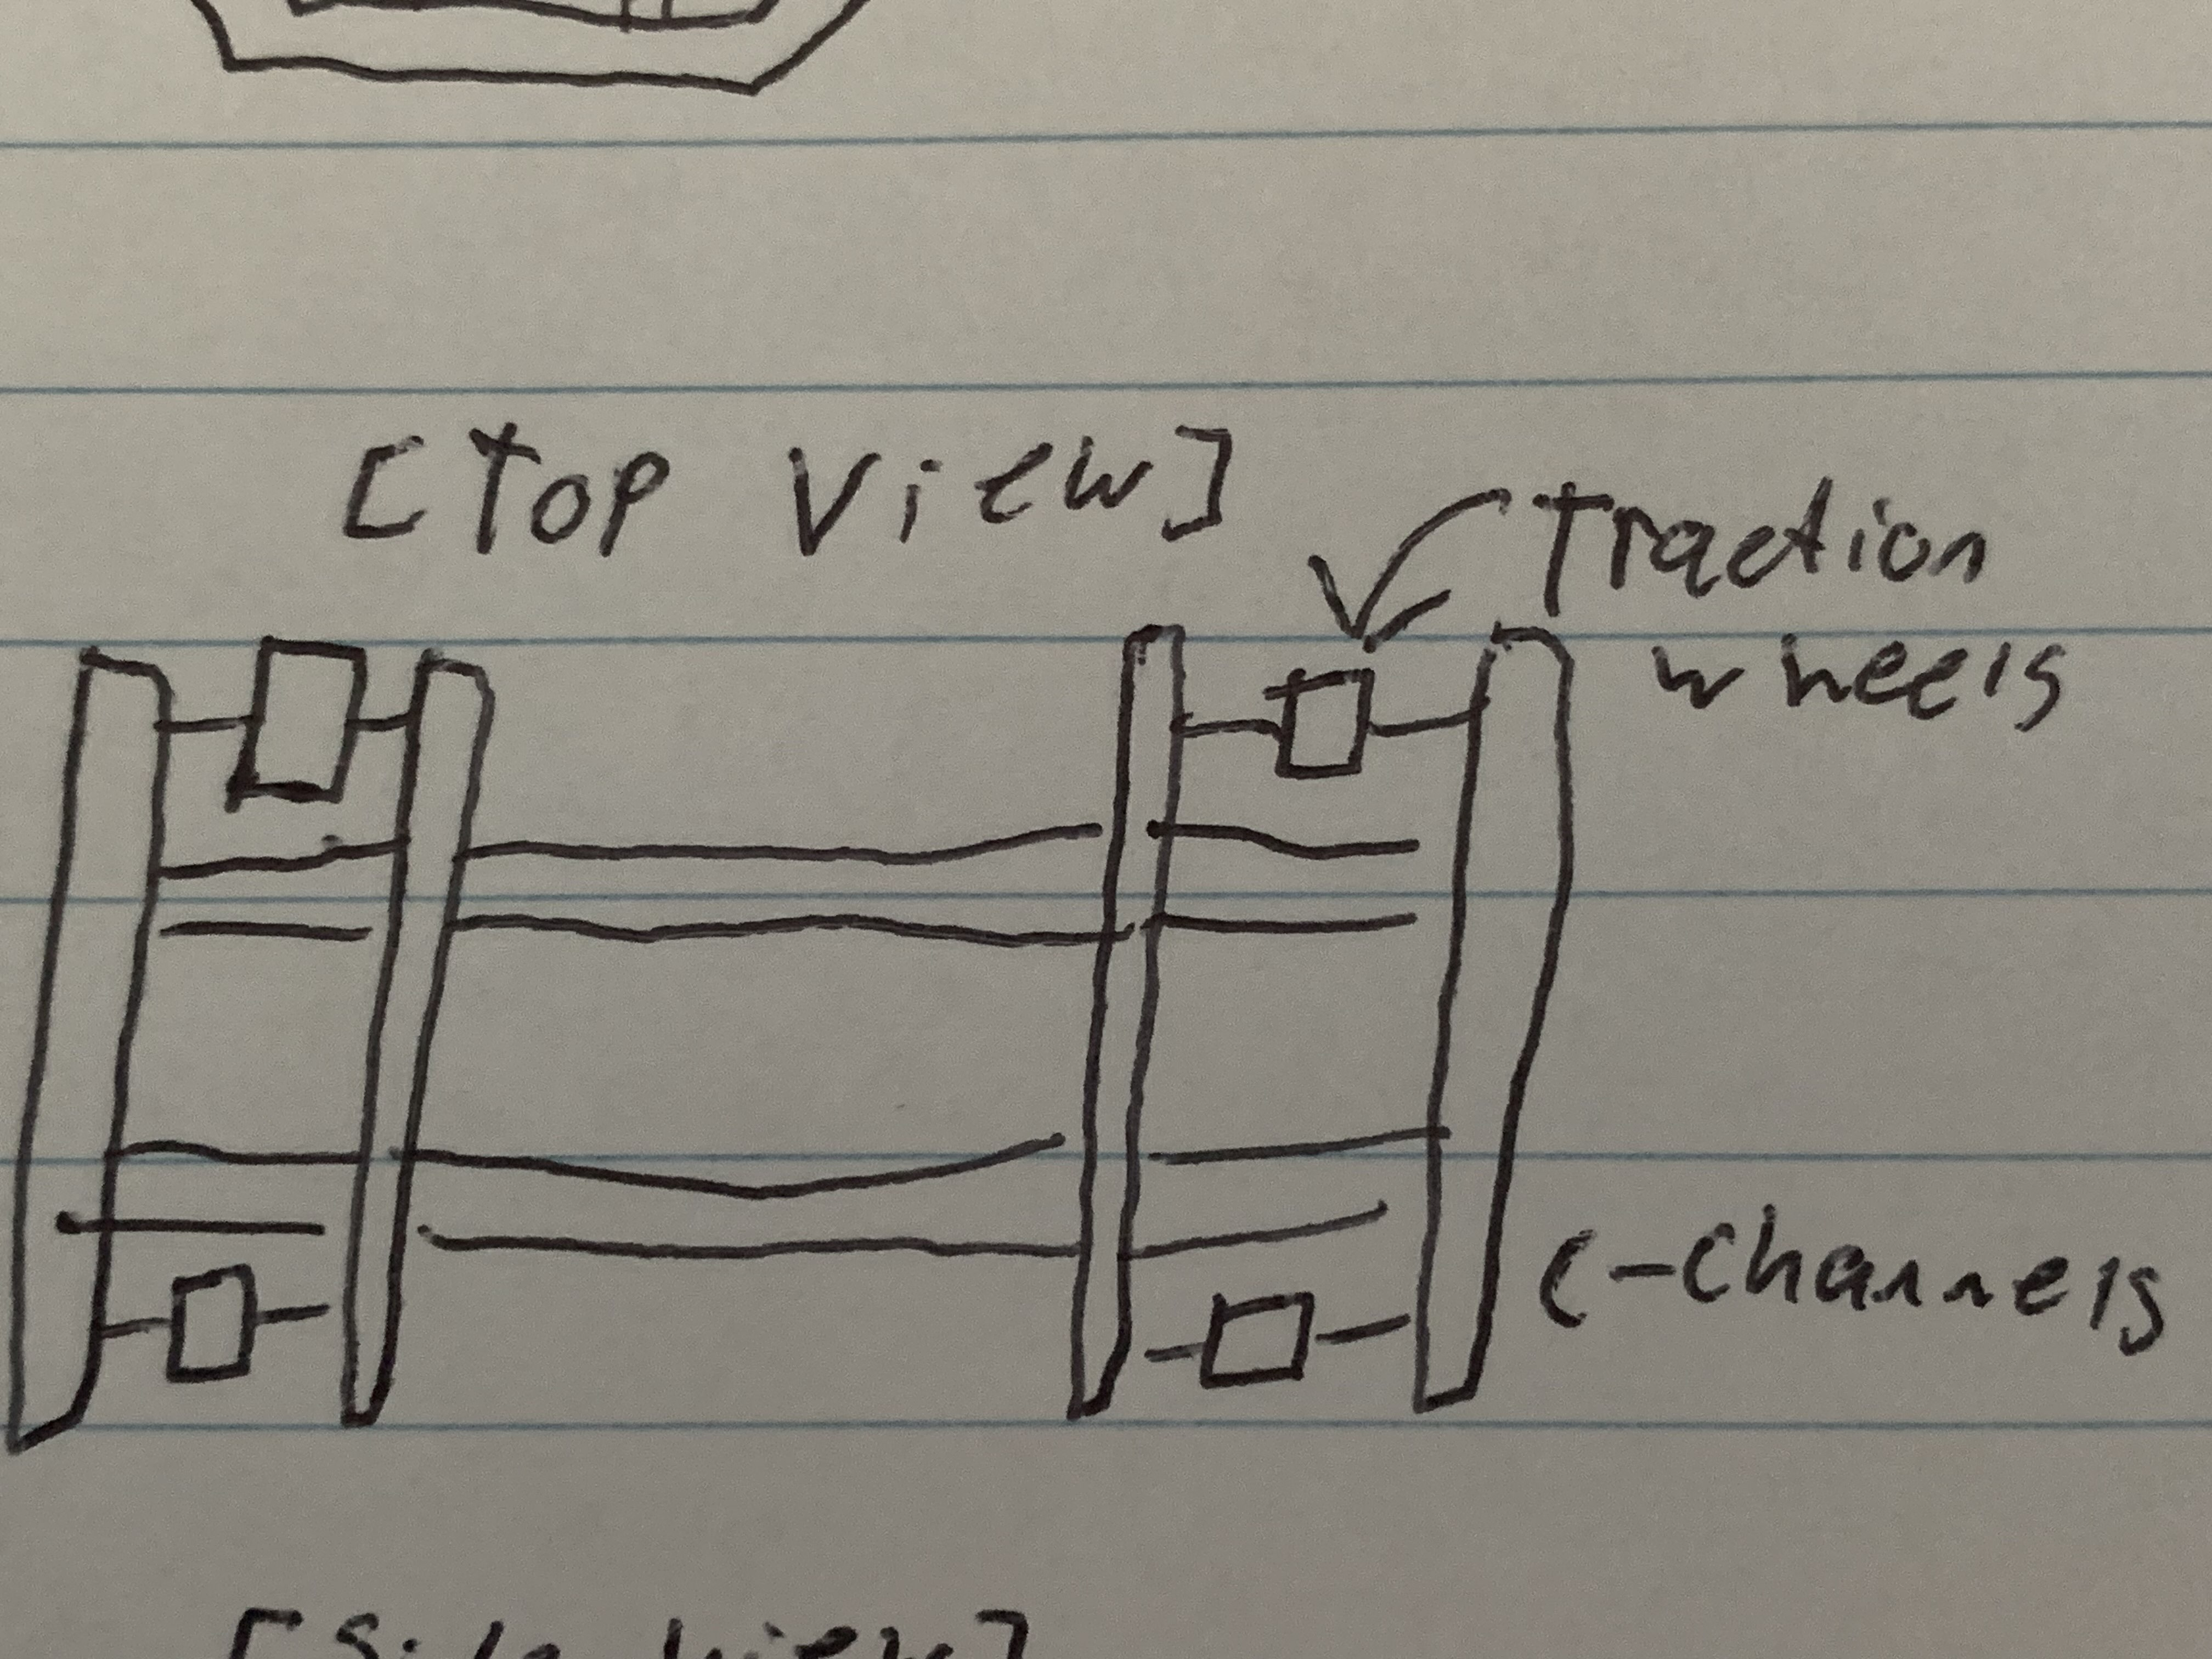
\includegraphics[width=.8\linewidth]{images/Traction Wheel Drive.jpg}
        \caption{Traction Wheel Drive}
        \label{fig:traction-wheel-drive}
    \end{minipage}%
    \begin{minipage}{.5\textwidth}
        \centering
        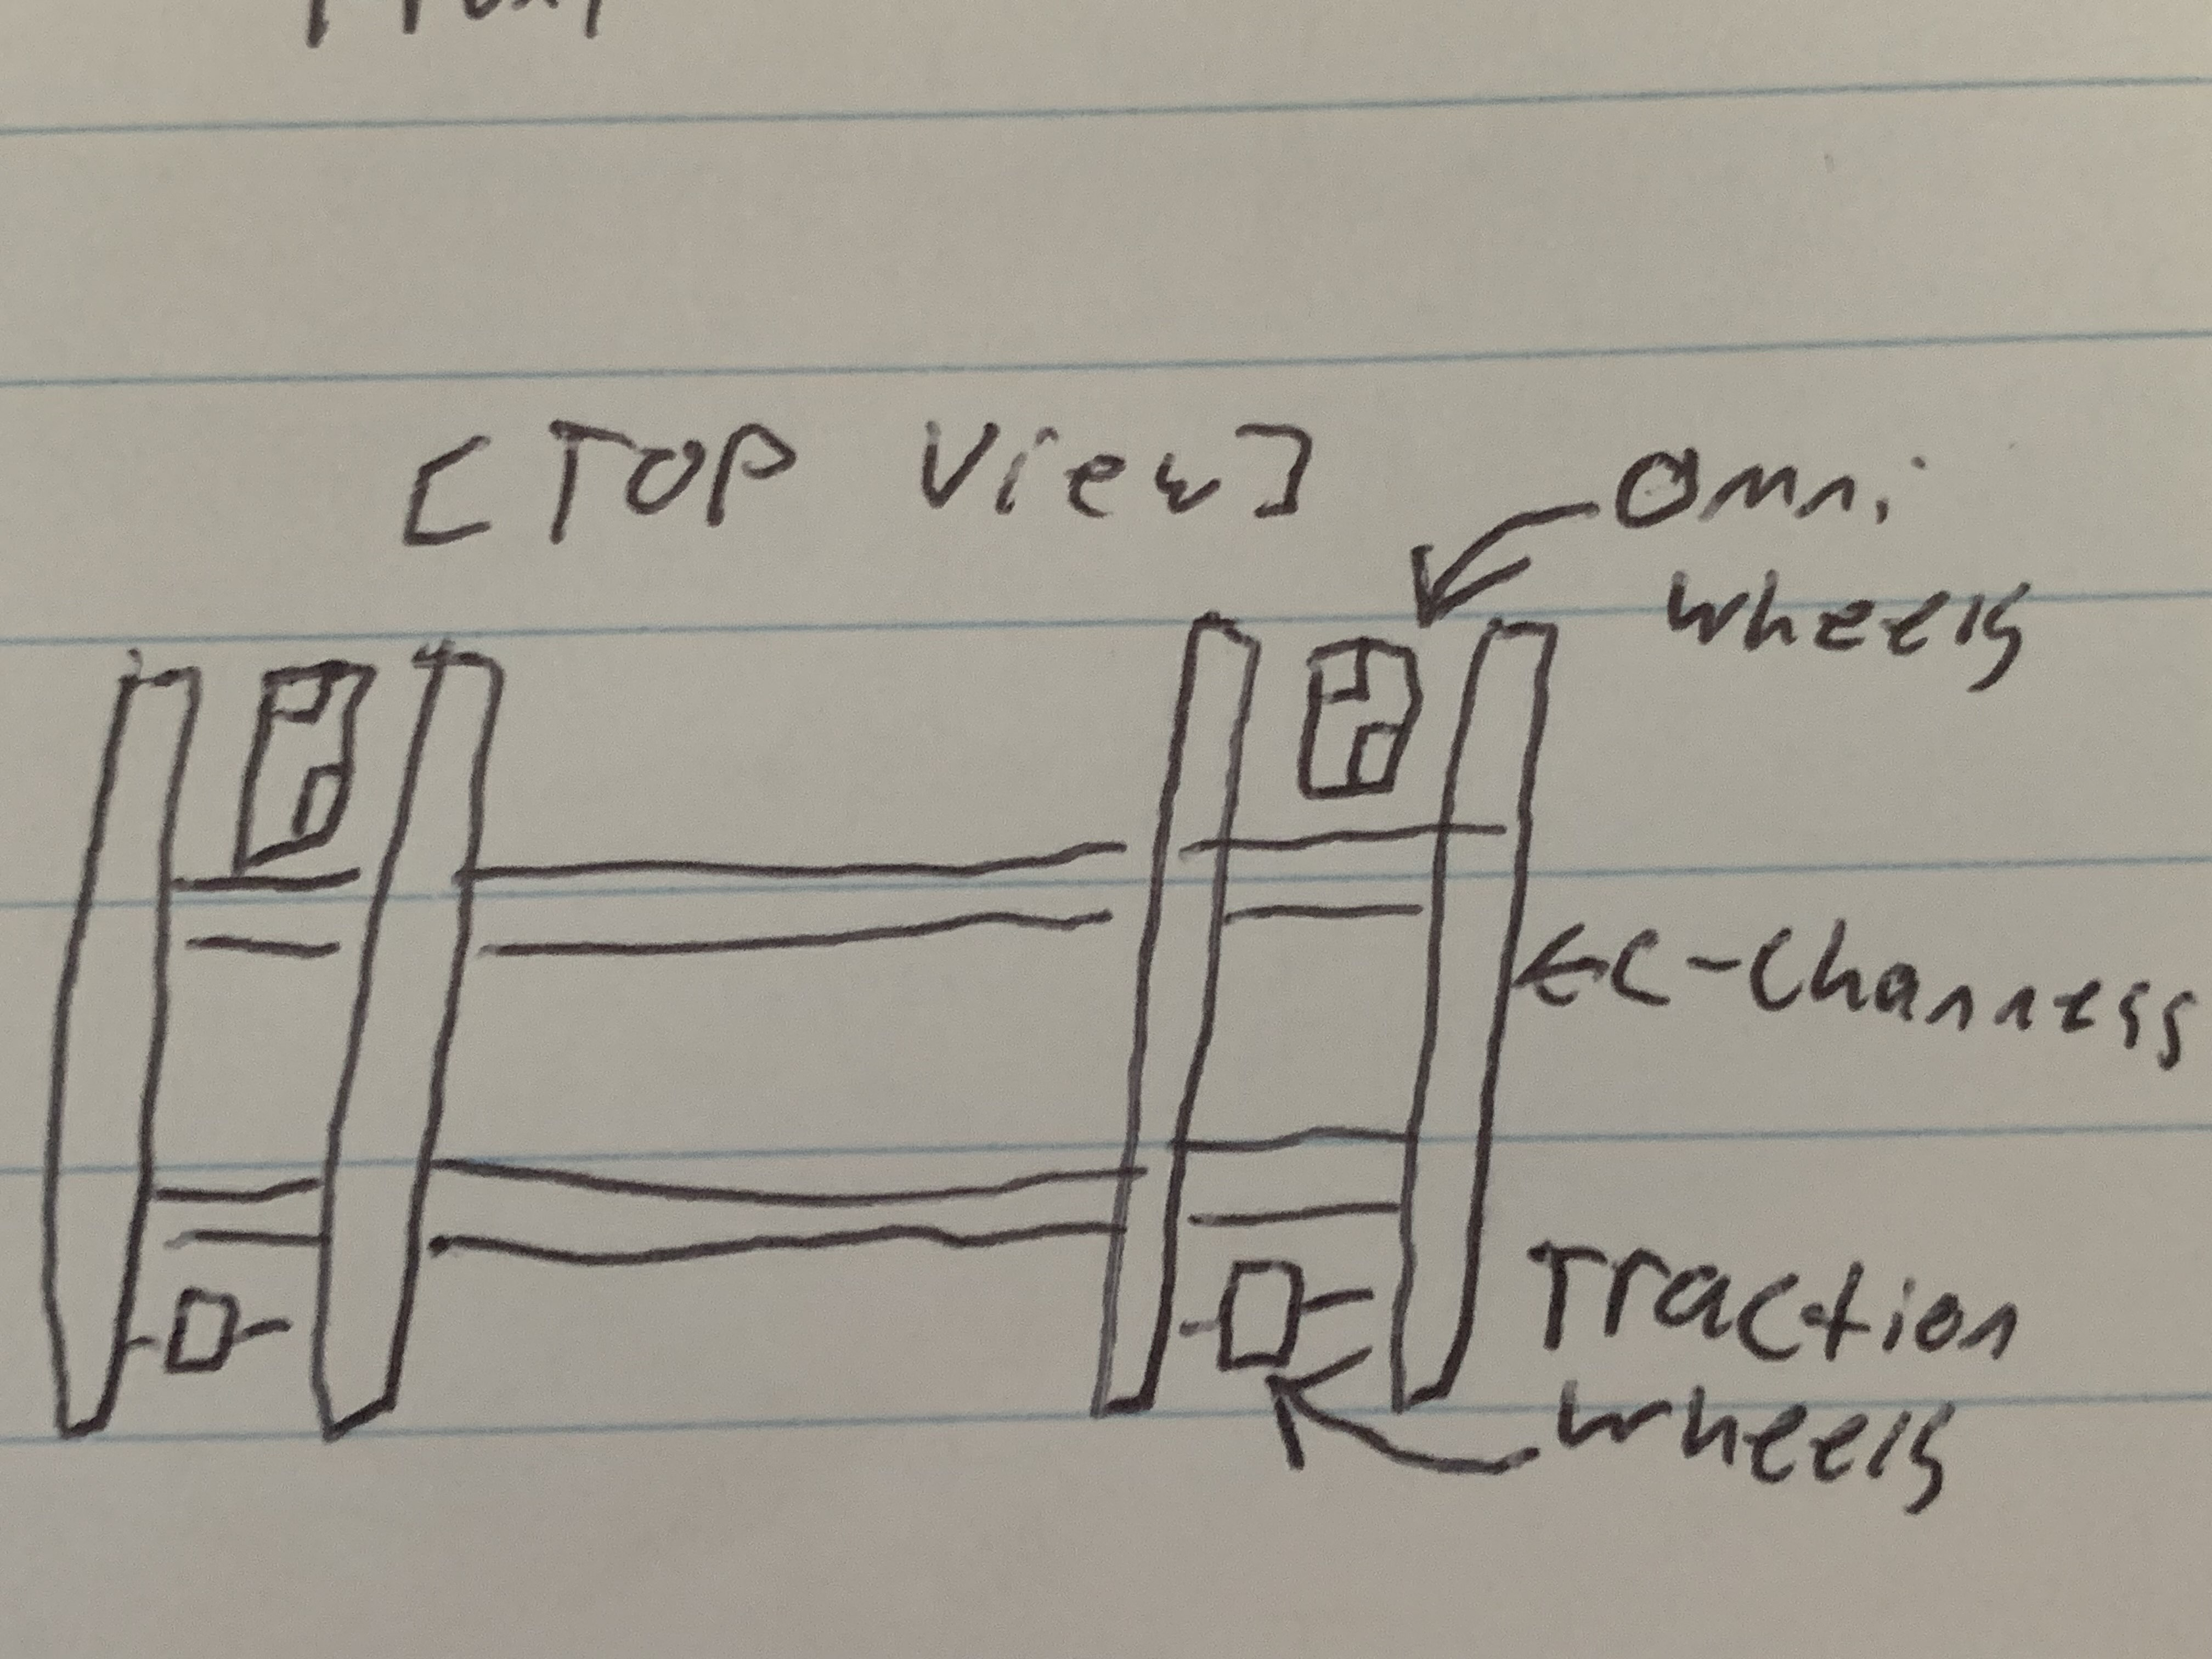
\includegraphics[width=.8\linewidth]{images/Omni and Traction Wheel Drive.jpg}
        \caption{Omnidirectional and Traction Wheels} %redraw this to look like our drive setup, traction in the middle and omnis on the outside
        %on it
        \label{fig:omnidirectional-and-traction-wheels}
    \end{minipage}
     \begin{minipage}{.5\textwidth}
        \centering
        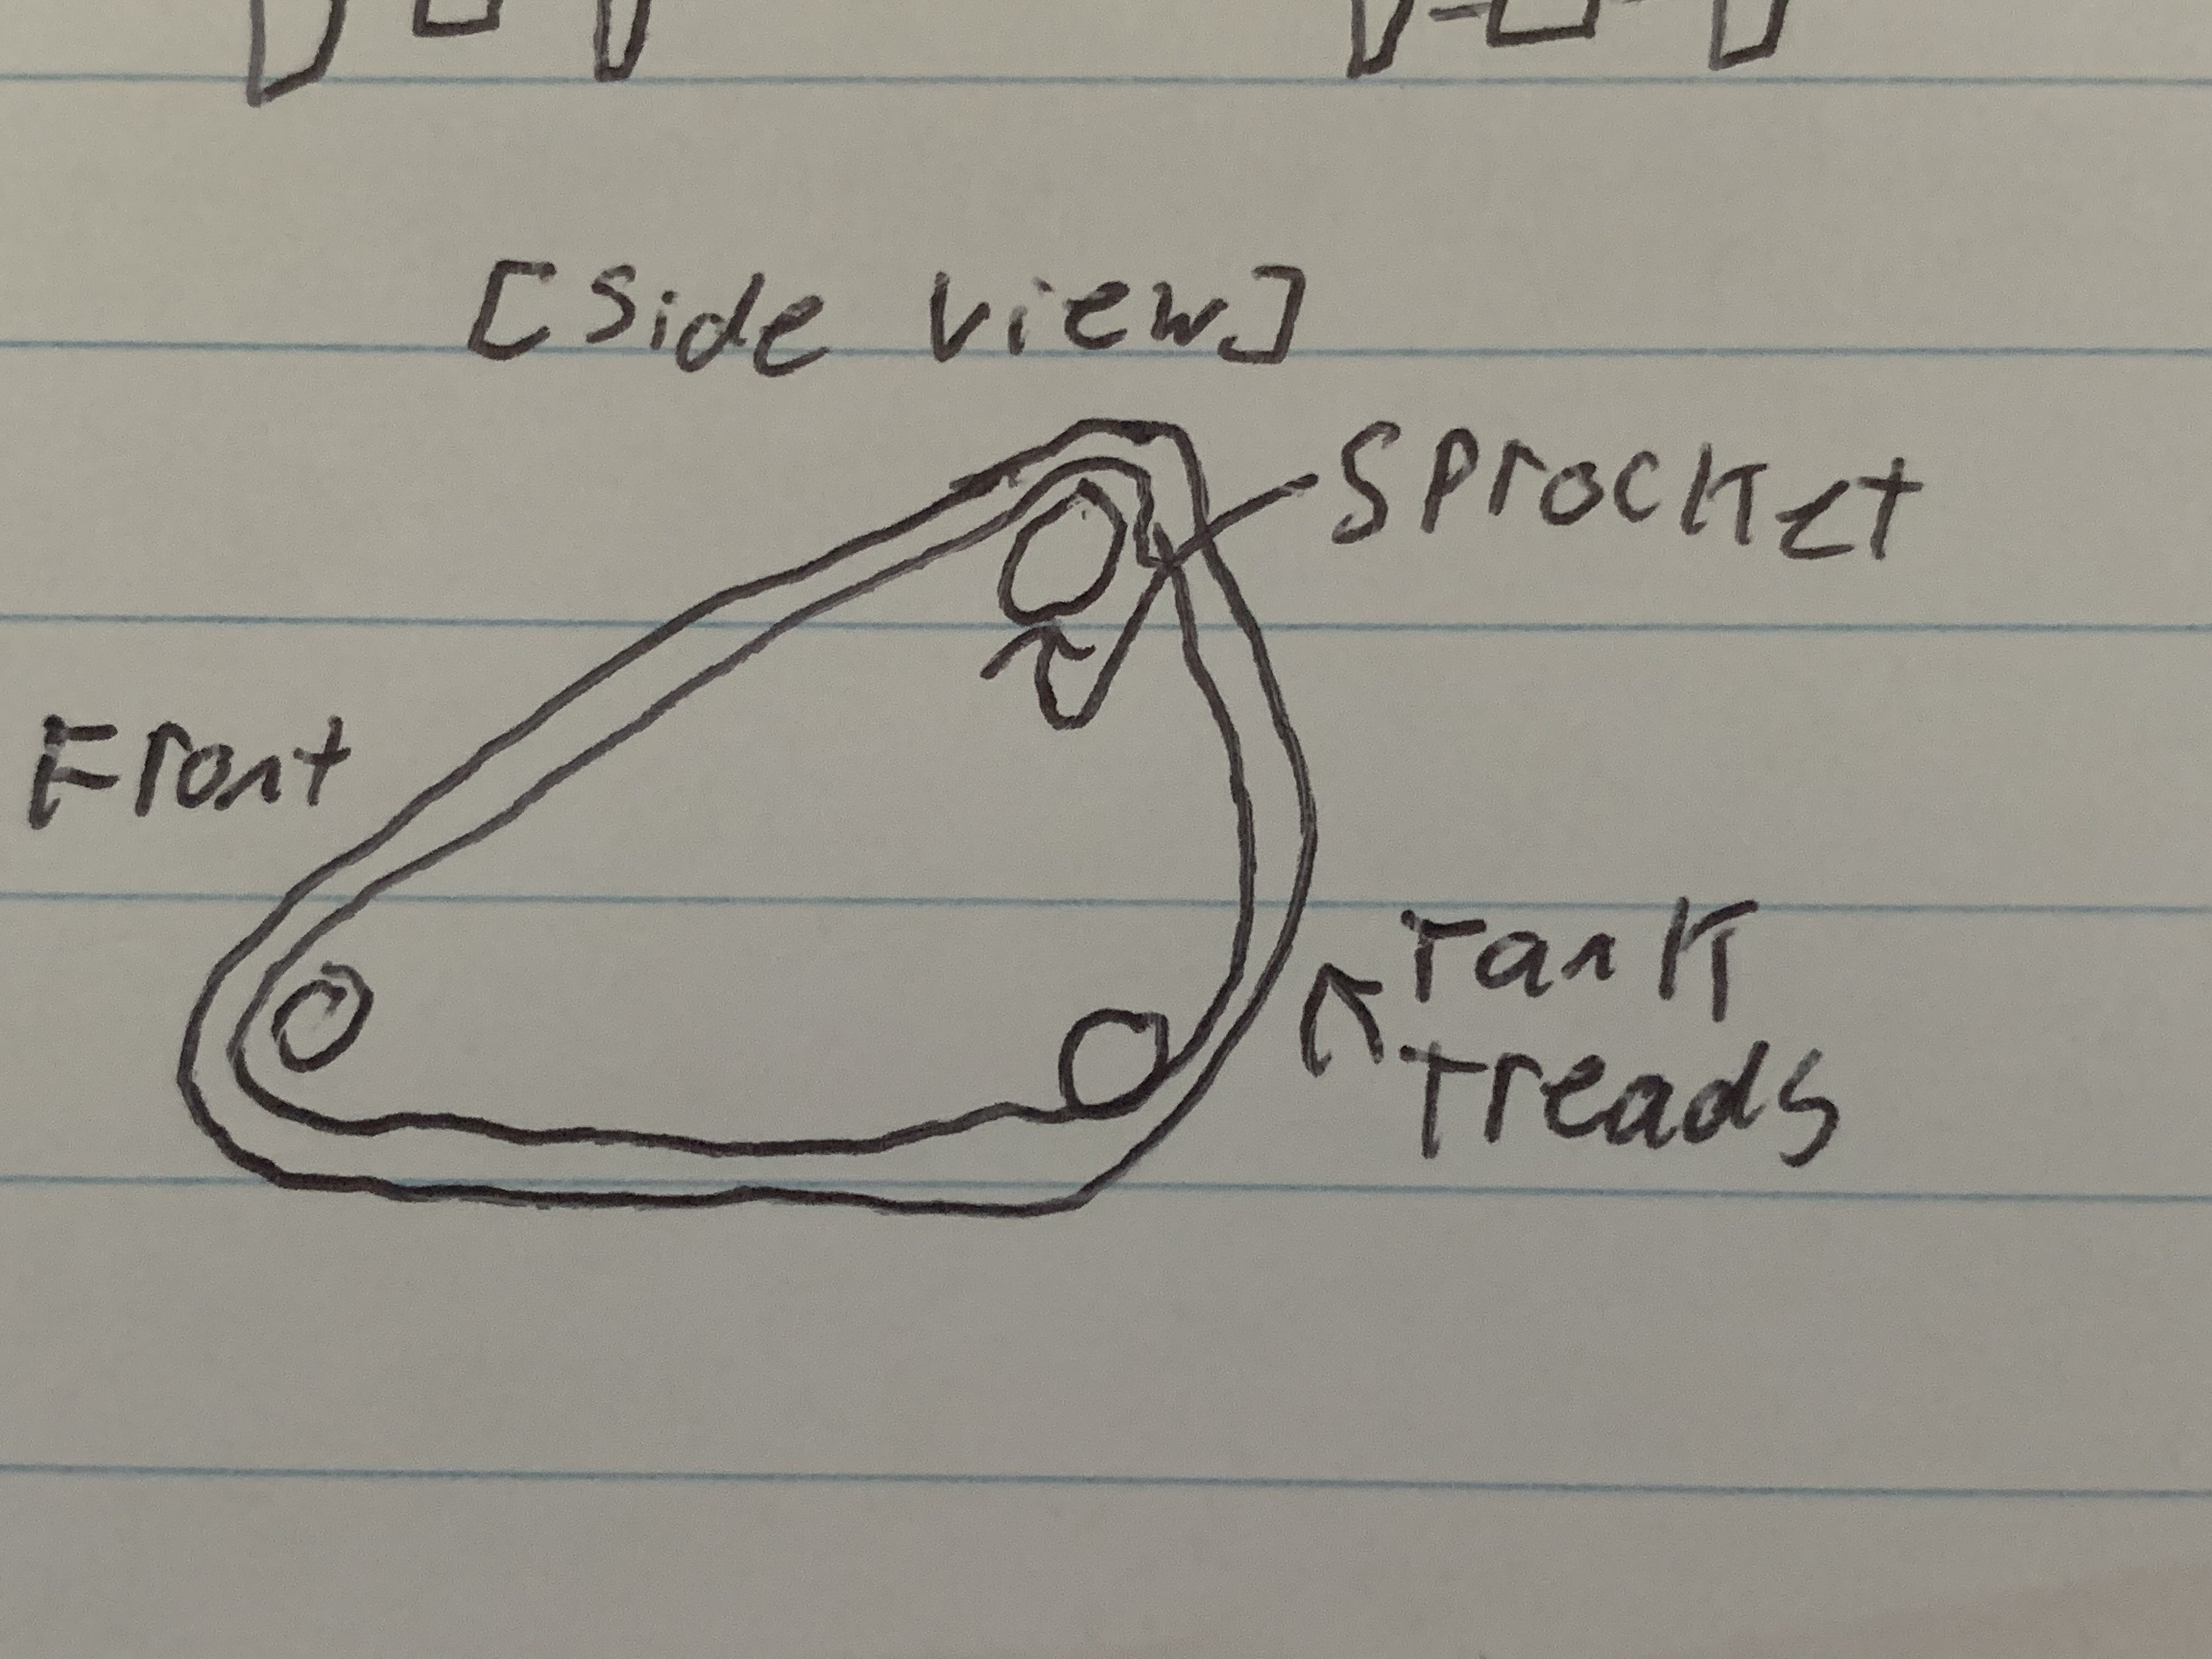
\includegraphics[width=.8\linewidth]{images/Tank - Treads.jpg}
        \caption{Tank Treads}
        \label{fig:tank-treads}
    \end{minipage}
     \begin{minipage}{.5\textwidth}
        \centering
        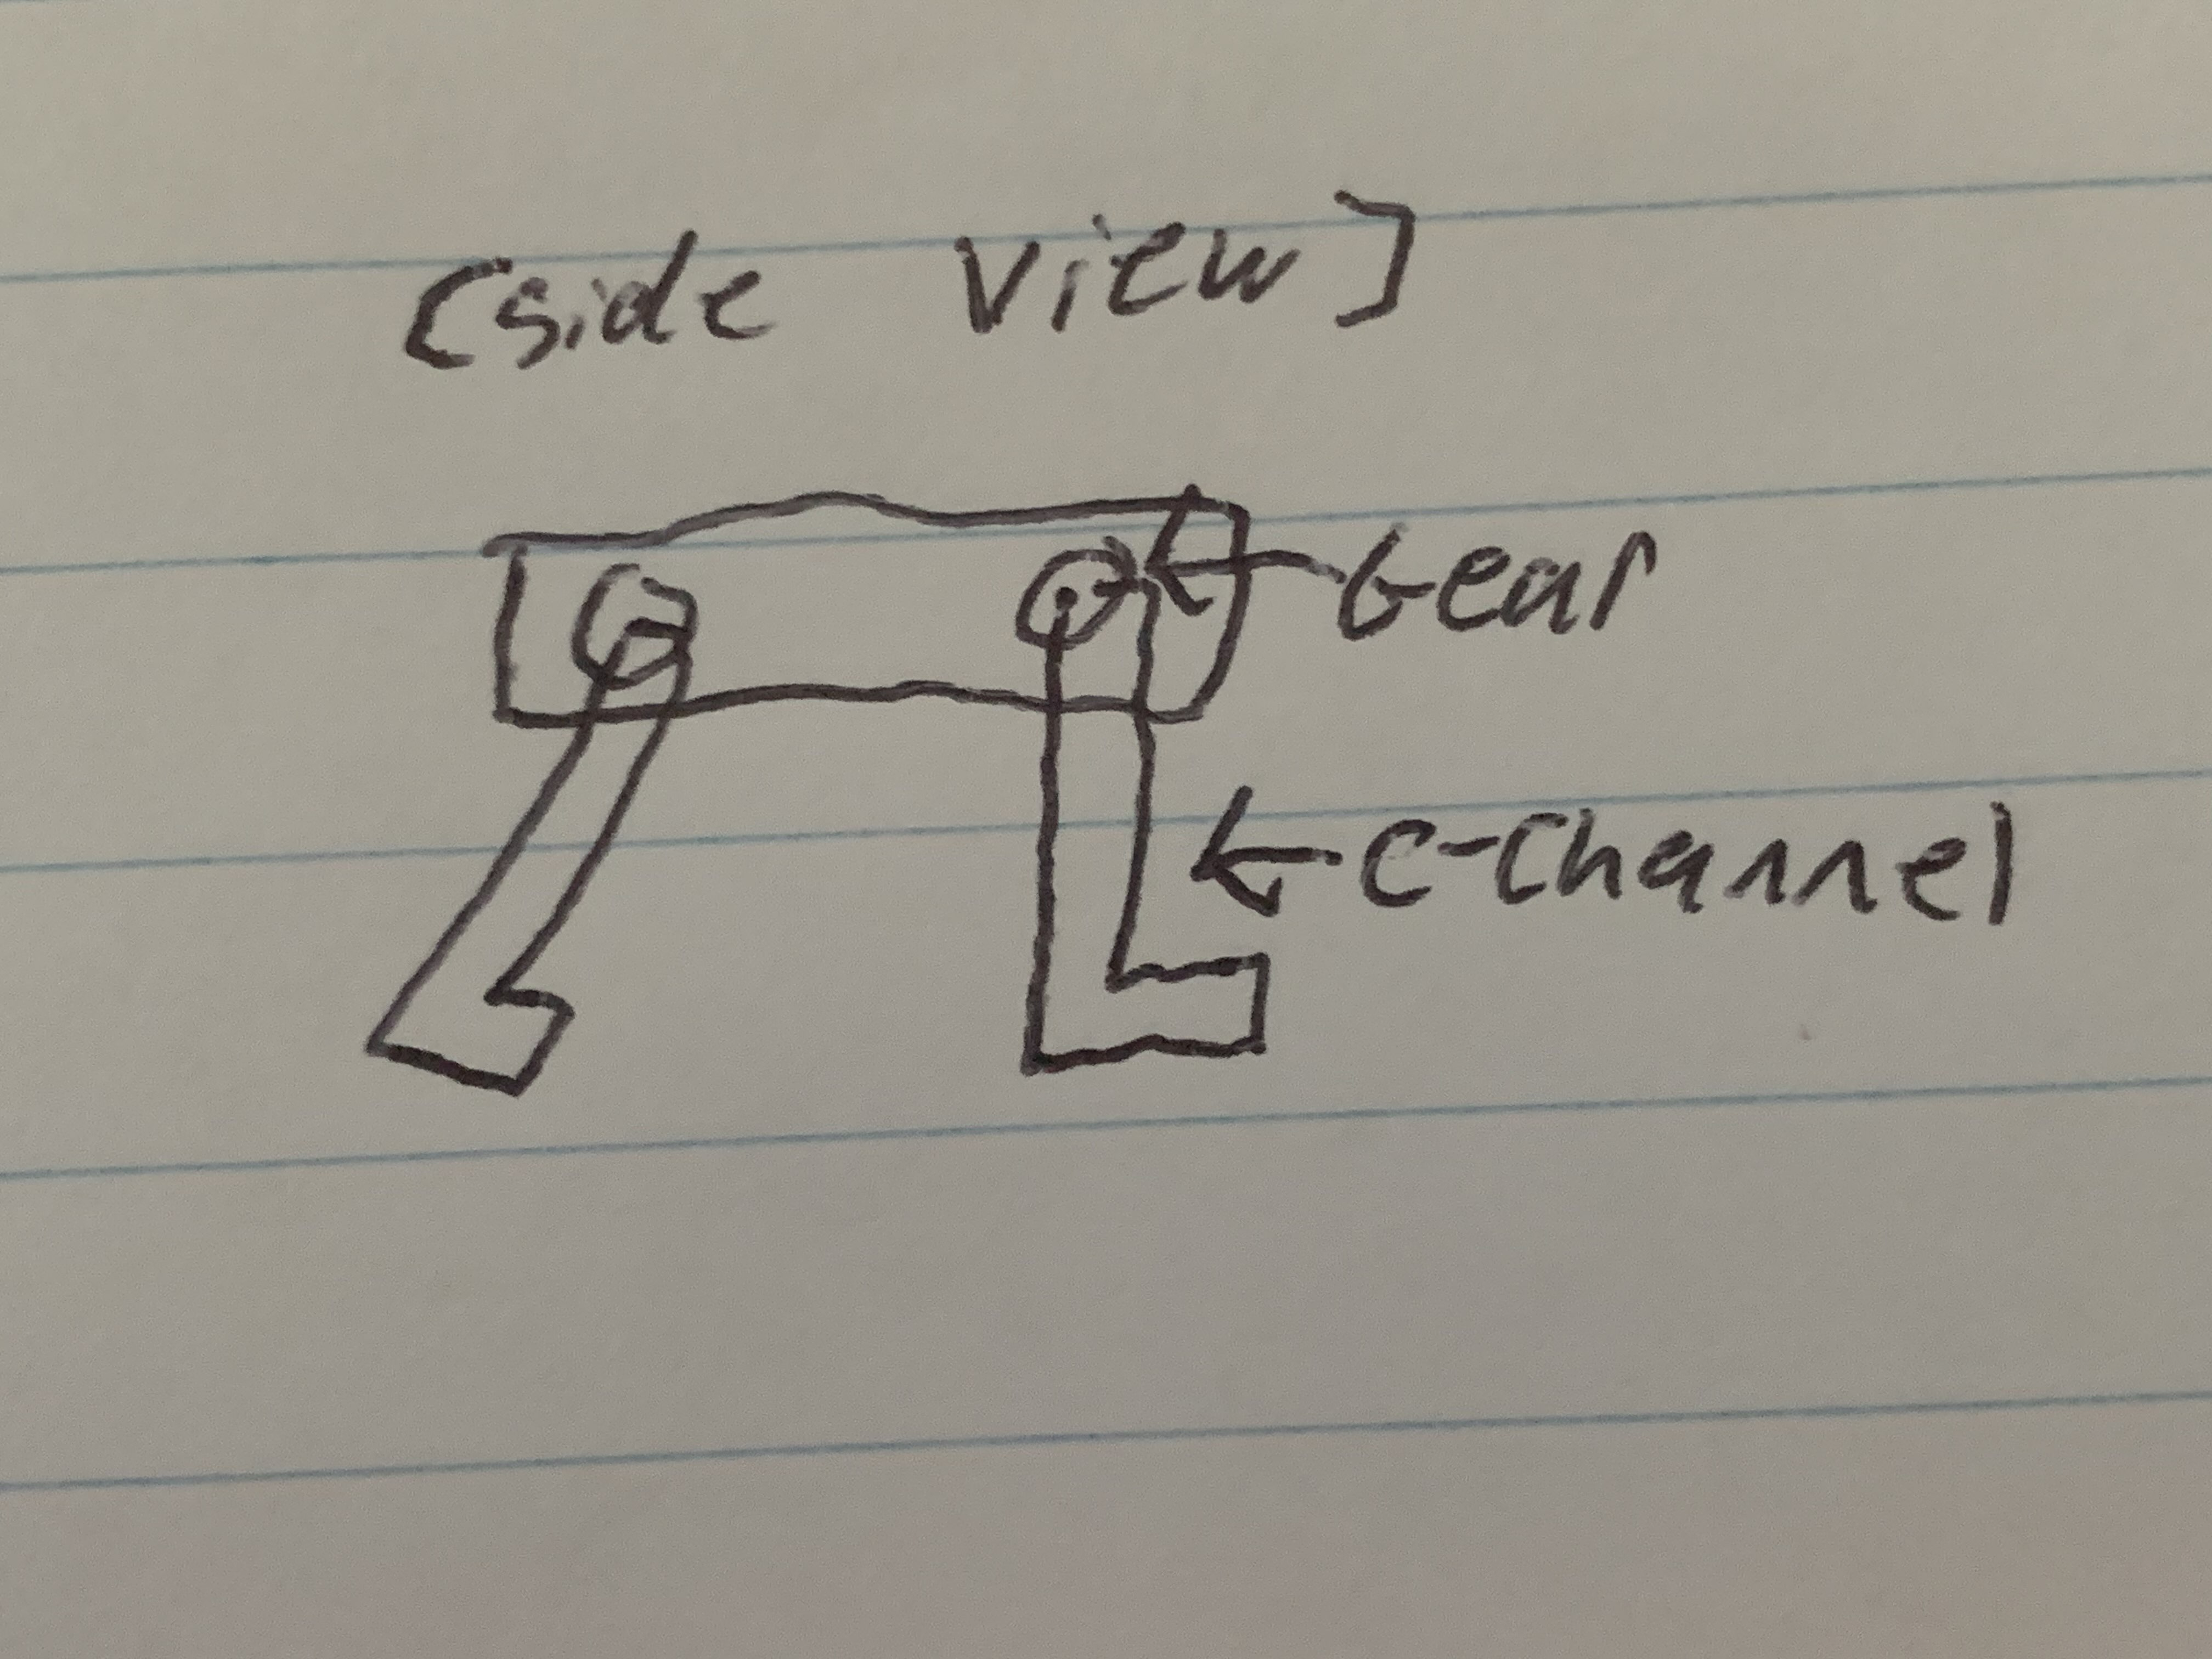
\includegraphics[width=.8\linewidth]{images/Walking Robot.jpg}
        \caption{Walking Robot}
        \label{fig:walking-robot}
    \end{minipage}
\end{figure}
\pagebreak
\white{June 2024}
\begin{center}
    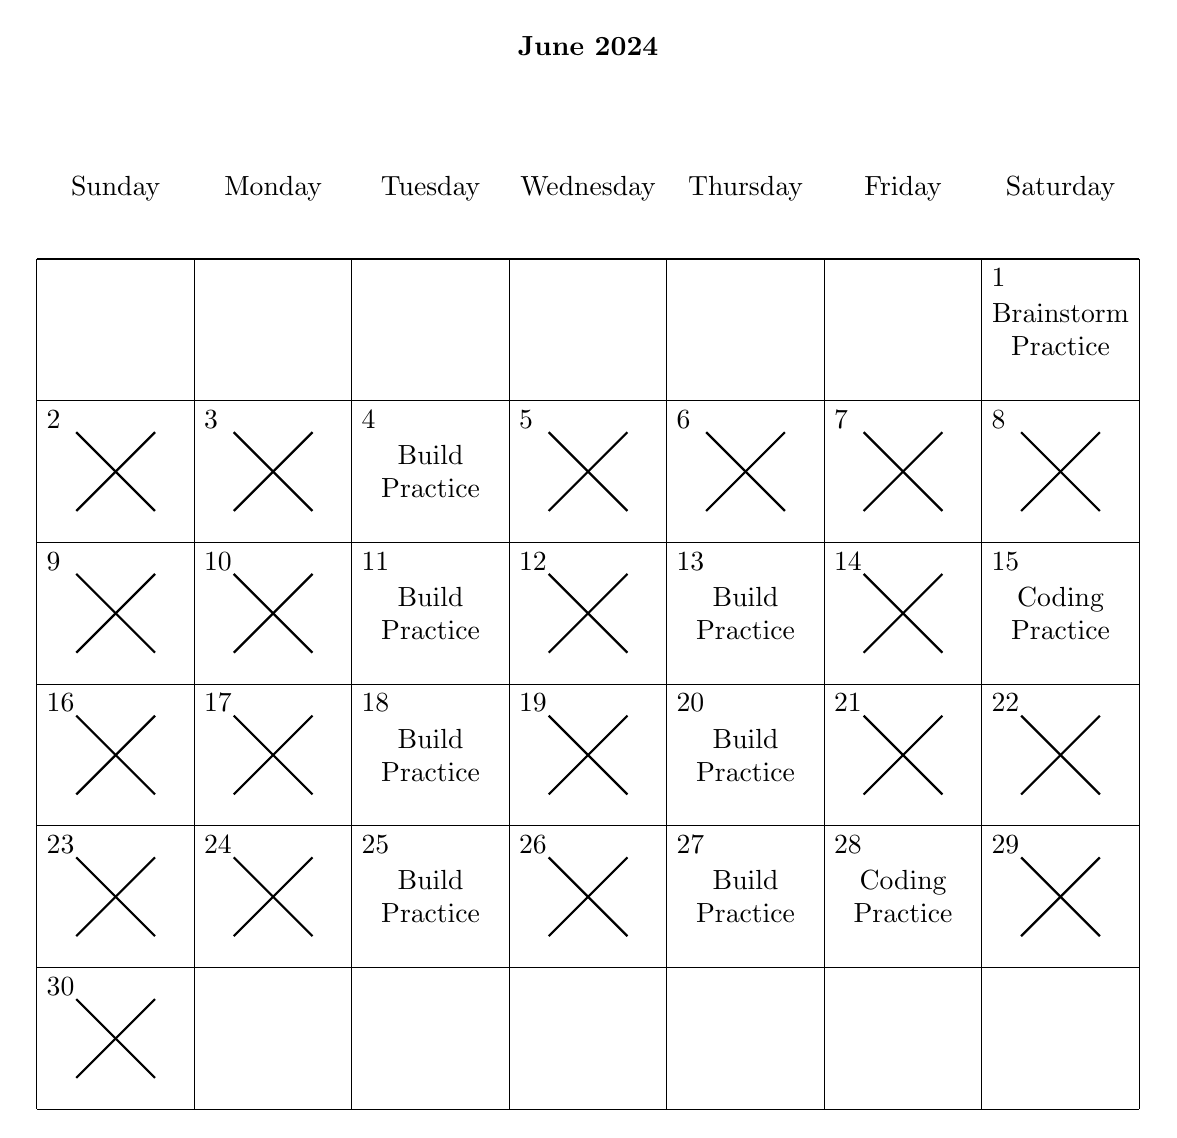
\begin{tikzpicture}
        % Define the dimensions of the calendar
        \def\year{2024}
        \def\month{6}
        \def\monthname{June}
        \def\startday{7} % 1=Sunday, 2=Monday, ..., 7=Saturday
        \def\numdays{30}
        \def\boxwidth{2} % Width of each box
        \def\boxheight{1.8} % Height of each box

\newcommand{\daytext}[1]{
    \ifcase#1
    \or Brainstorm Practice \or \cross  \or \cross \or  Build Practice \or  \cross \or  \cross \or  \cross \or \cross \or  \cross \or \cross
    \or Build Practice \or  \cross \or Build Practice \or  \cross \or Coding Practice \or  \cross \or \cross \or Build Practice \or  \cross \or Build Practice
    \or  \cross \or \cross \or  \cross \or \cross \or Build Practice \or \cross \or Build Practice \or Coding Practice \or \cross \or  \cross
    \or \cross
    \fi
}

        % Draw the calendar grid
        \foreach \x in {0, 1, 2, 3, 4, 5, 6, 7} {
            \draw (\x*\boxwidth, 0) -- (\x*\boxwidth, -6*\boxheight);
        }
        \foreach \y in {0, -1, -2, -3, -4, -5, -6} {
            \draw (0, \y*\boxheight) -- (7*\boxwidth, \y*\boxheight);
        }

        % Add day labels
        \node at (0.5*\boxwidth, 0.5*\boxheight) {Sunday};
        \node at (1.5*\boxwidth, 0.5*\boxheight) {Monday};
        \node at (2.5*\boxwidth, 0.5*\boxheight) {Tuesday};
        \node at (3.5*\boxwidth, 0.5*\boxheight) {Wednesday};
        \node at (4.5*\boxwidth, 0.5*\boxheight) {Thursday};
        \node at (5.5*\boxwidth, 0.5*\boxheight) {Friday};
        \node at (6.5*\boxwidth, 0.5*\boxheight) {Saturday};

        % Add the dates in the top left corner and specific text in the middle
        \foreach \d in {1,...,\numdays} {
            \pgfmathtruncatemacro{\col}{mod(\d+\startday-2, 7)}
            \pgfmathtruncatemacro{\row}{-(\d+\startday-2)/7}
            \node[anchor=north west] at (\col*\boxwidth, \row*\boxheight) {\d};
            \node[anchor=center, text width=\boxwidth cm, align=center] at (\col*\boxwidth+0.5*\boxwidth, \row*\boxheight-0.5*\boxheight) {\daytext{\d}};
        }

        % Add month and year
        \node at (3.5*\boxwidth, 1.5*\boxheight) {\textbf{\monthname\ \year}};
    \end{tikzpicture}
\end{center}
This is our what happened during the month of June. We had full team meetups every Tuesday and every Thursday except for June the 6th. Connor had the robot during this time, Ian has been working on the AI, and Jayden has been working on the simulator, which will have a full chapter on it once in place. At the end of the month we had just finished the Clamp. 
\solution{Choose a Solution \& Make a Plan: Drivetrain (June 3, 2024}
\label{Choose-a-Solution-&-Make-a-Plan:-Drivetrain}
\chapterauthor{Caleb Bachmeier}
\info{Caleb Bachmeier}{Choose a Solution \& Make a Plan: Drivetrain}{June 3, 2024}
\textbf{Goal}: Choose which solution to use for our drivetrain
    \section*{Choose a Solution}
\subsection*{Decision Matrix}
On the following page is a (\blueref{tab:drive-matrix}{decision matrix}). A decision matrix, also known as a decision-making grid, is a systematic tool used to evaluate and prioritize a set of options based on a predefined set of criteria. It's particularly useful in engineering and other technical fields where decisions often involve weighing multiple factors or criteria. Which is why we've decided to use one to decide which type of drive to use. The team has already ruled out Mecanum, X-Drive, Tank Treads, and Walking Robot because we've never seen any top teams use those types of drives. The row "Weight" determines how much weight a specific column revives in terms of points. It wouldn't be fair to compare the size of the robot and the speed 1-1 because speed is much more important than size.
\pagebreak
\renewcommand{\arraystretch}{1.85} % Change this value as needed
\begin{table}[htb!]
\centering
\begin{tabular}{|>{\centering\arraybackslash}m{1.85cm}|>{\centering\arraybackslash}m{1.85cm}|>{\centering\arraybackslash}m{1.85cm}|>{\centering\arraybackslash}m{1.85cm}|>{\centering\arraybackslash}m{1.85cm}|>{\centering\arraybackslash}m{1.85cm}|>{\centering\arraybackslash}m{1.85cm}|}
\hline
\textbf{Scale 1 - 10} & \textbf{Complexity} & \textbf{Motors Needed} & \textbf{Traction} & \textbf{Size} & \textbf{Speed} & \textbf{Total} \tabularnewline
\hline
Weight & x1 & x3 & x2 & x1 & x3 & \tabularnewline
\hline
Standard Omni & 10 & 10 & 6 & 10 & 6 & 88 \tabularnewline
\hline
Omni and Traction & 10 & 10 & 10 & 10 & 8 & 94 \tabularnewline
\hline
Traction & 10 & 10 & 10 & 10 & 4 & 74 \tabularnewline
\hline
H-Drive & 6 & 8 & 6 & 10 & 6 & 70 \tabularnewline
\hline
\end{tabular}
\caption{Drive Decision Matrix}
\label{tab:drive-matrix}
\end{table}
\renewcommand{\arraystretch}{1.85} % Reset to default

Looking at the point totals, it seems that a Omnidirectional and Traction wheel drive is our best option.
\subsection*{Brainstorm}
Using a Traction and Omnidirectional wheel drive, our initial design incorporated a 600 RPM drive with 2.75-inch wheels, which satisfied our baseline speed criteria. However, a subsequent CAD analysis indicated that the 36-tooth gears in our original gearing arrangement resulted in insufficient spacing for idler gears due to the proximity of the wheels (\blueref{fig:600-RPM-clearance-issue}{600 RPM Clearance Issue}). In search of alternatives, we contemplated utilizing 48-tooth gears, but this adjustment extended the drive beyond our 15-inch maximum length constraint (\blueref{fig:48t-gears-=-too-long}). We then explored a 450 RPM drive with 2.75-inch wheels, which improved wheel spacing, but this configuration fell short of our velocity target, achieving only 64 inches/second—just below our 65 inches/second minimum threshold (\blueref{fig:450-on-3.25-issue}{450 RPM on 3.25 inches issue}). A switch to 3.25-inch wheels rectified the speed shortfall, but reintroduced the clearance problem encountered earlier.


\begin{center}
    \textbf{These are some are computer aided designs (CAD) using Fusion 360 of the problems listed above}
\end{center}
\begin{figure} [htb!]
    \begin{minipage}{.5\textwidth}
        \centering
        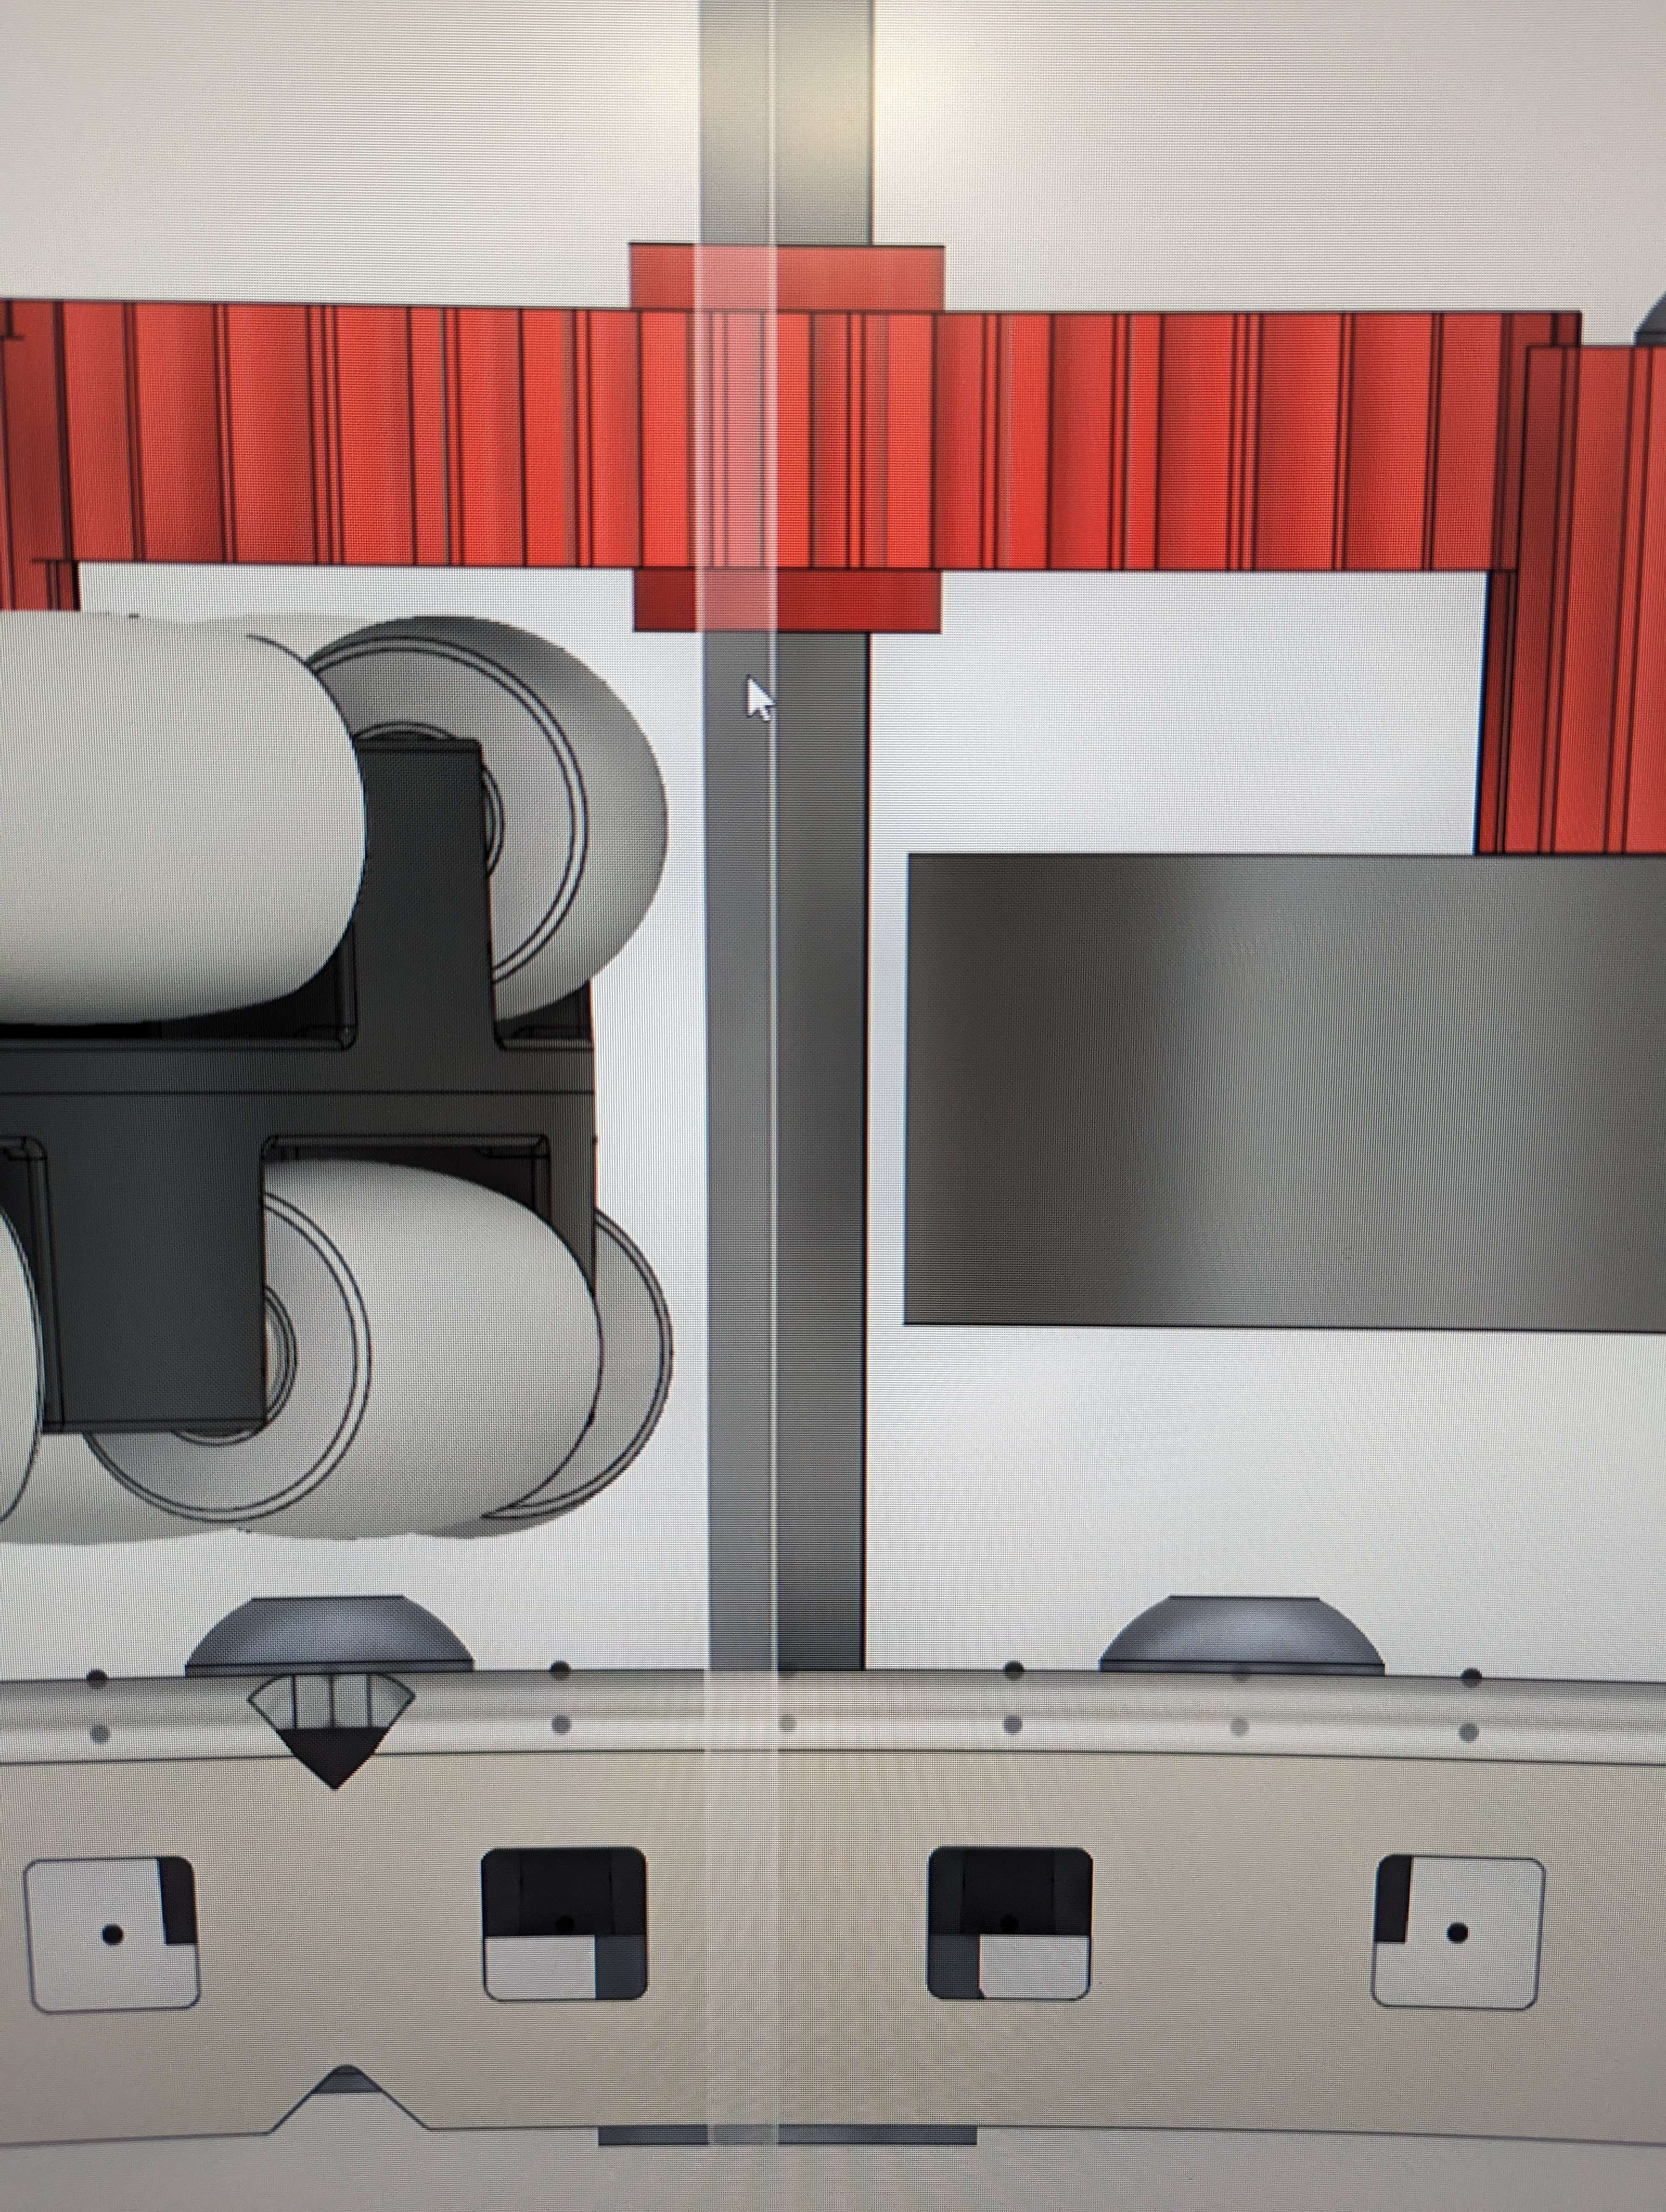
\includegraphics[width=.8\linewidth]{images/600 RPM Clearance Issue.jpg}
        \caption{600 RPM Clearance Issue}
        \label{fig:600-RPM-clearance-issue}
    \end{minipage}
    \begin{minipage}{.5\textwidth}
        \centering
        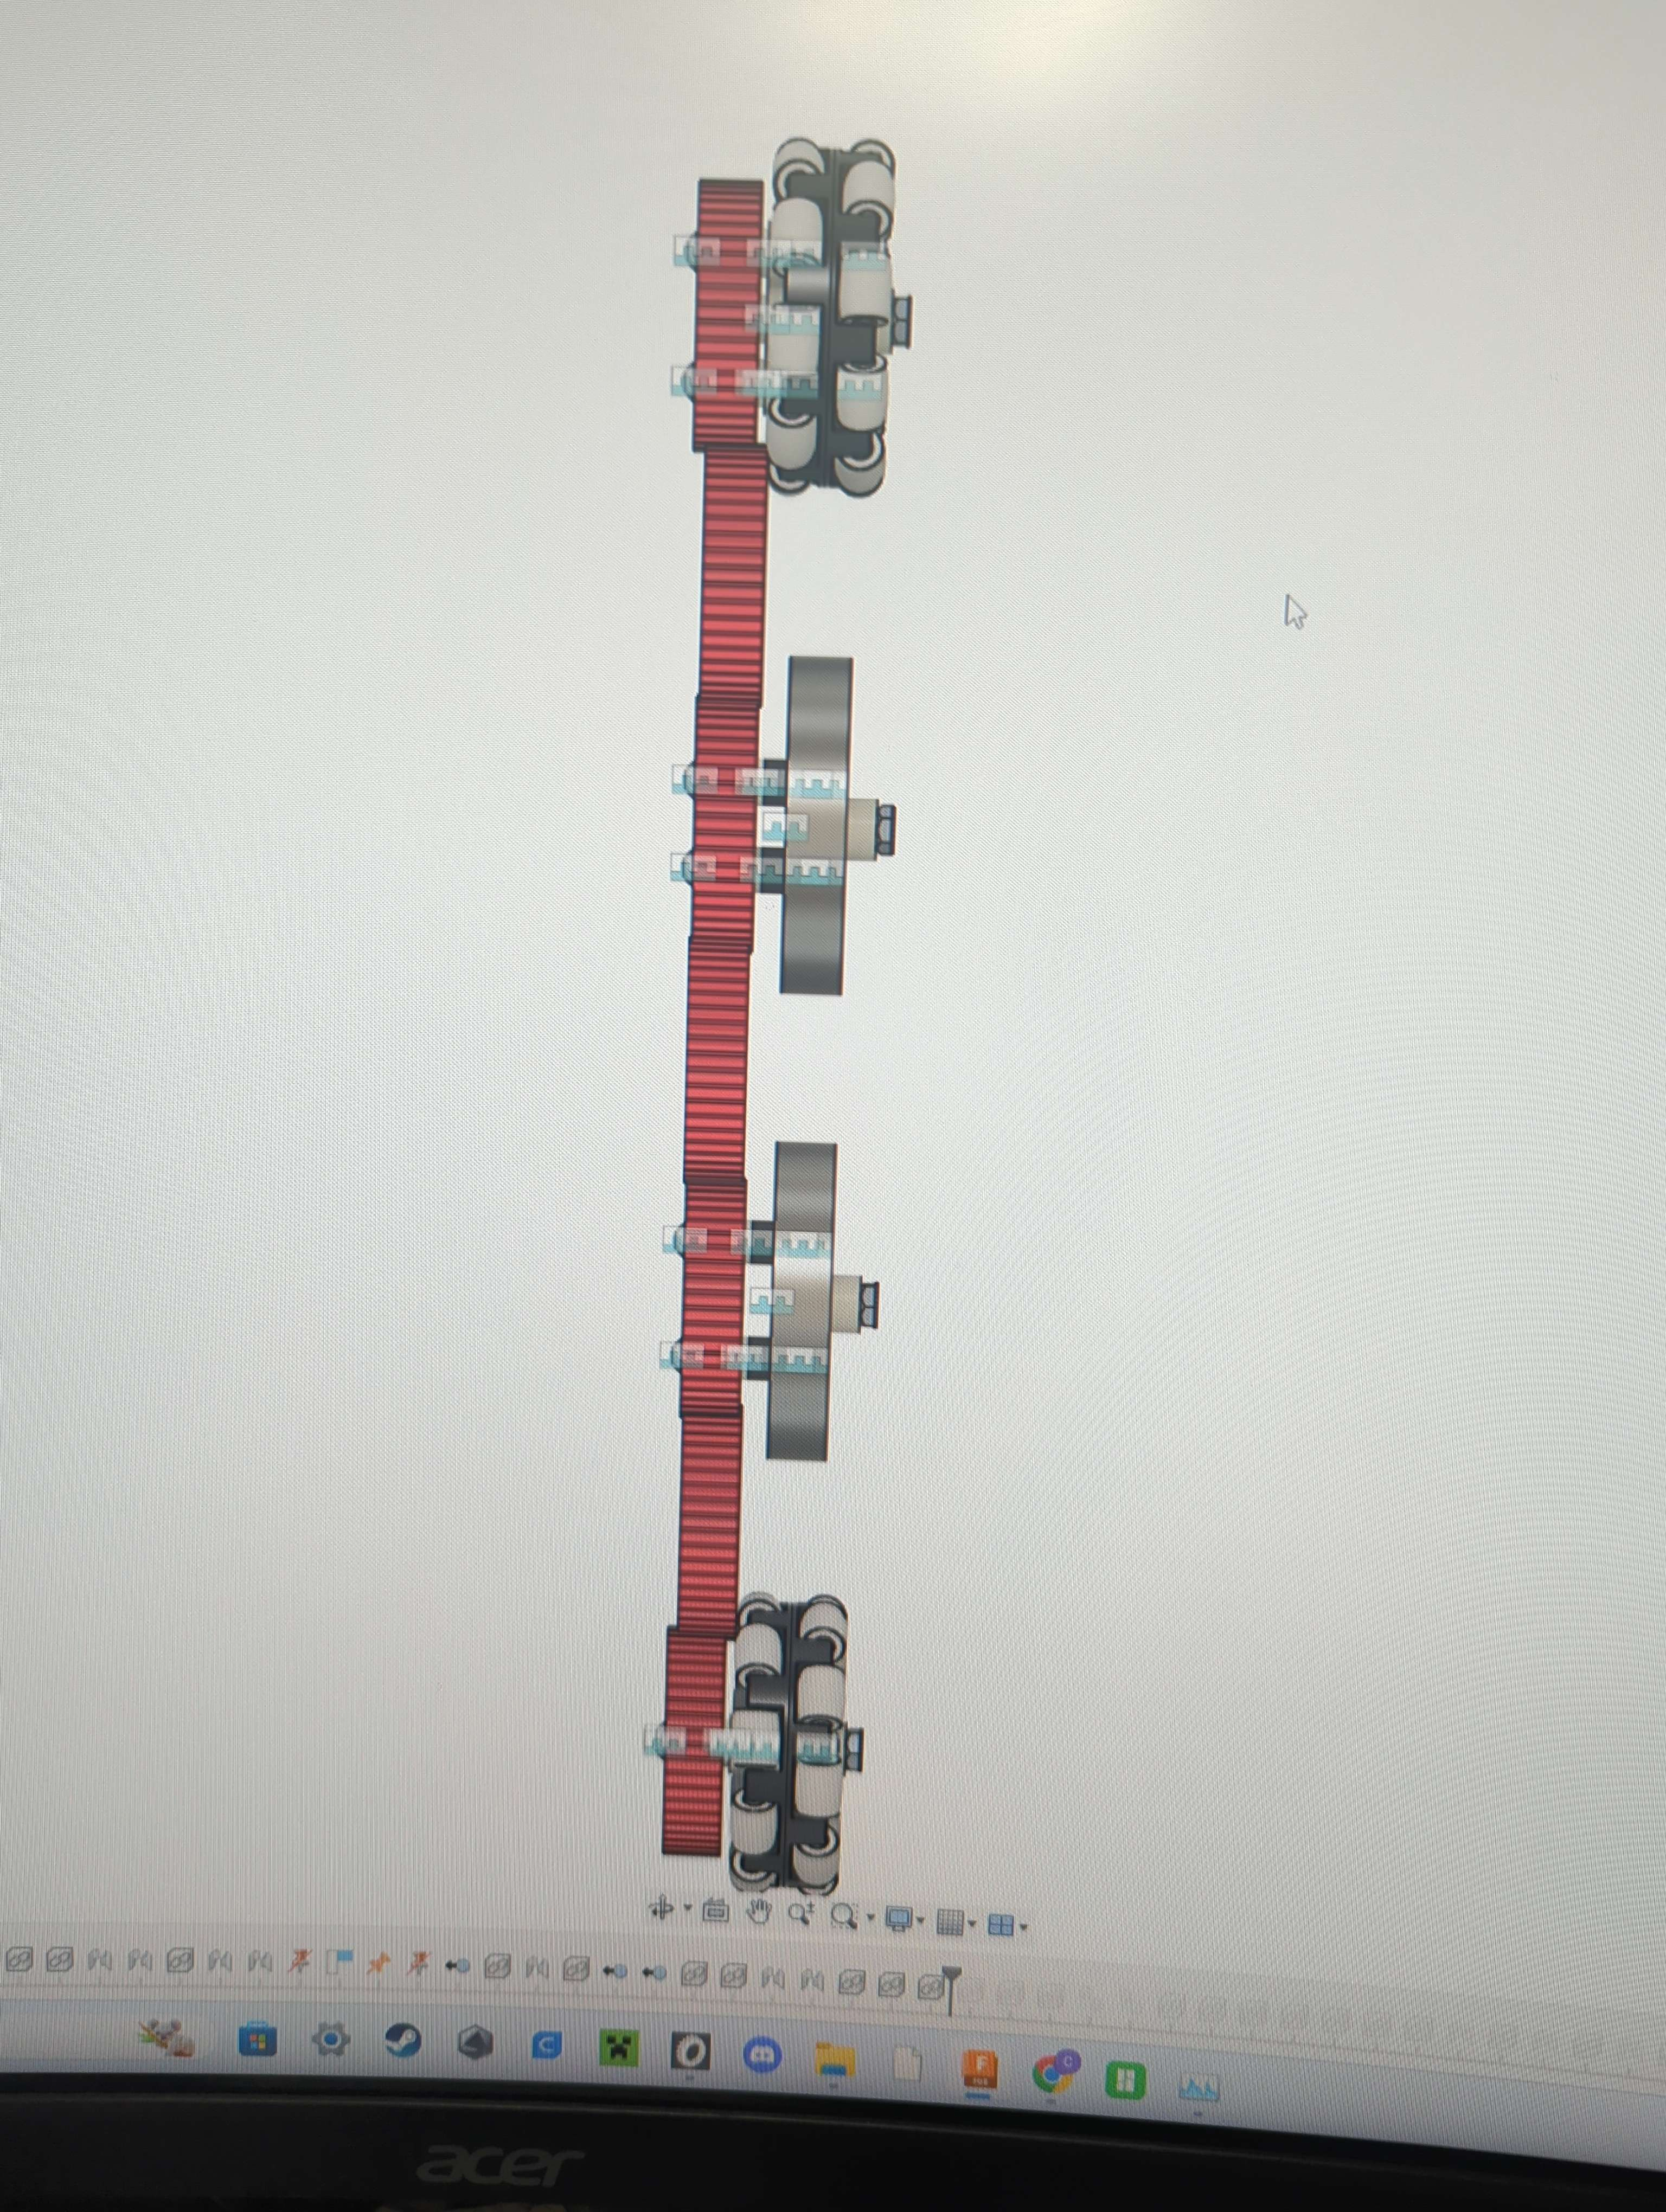
\includegraphics[width=.8\linewidth]{images/48t gears = too long.jpg}
        \caption{48 Tooth Gears}
        \label{fig:48t-gears-=-too-long}
    \end{minipage}
    \begin{minipage}{.5\textwidth}
        \centering
        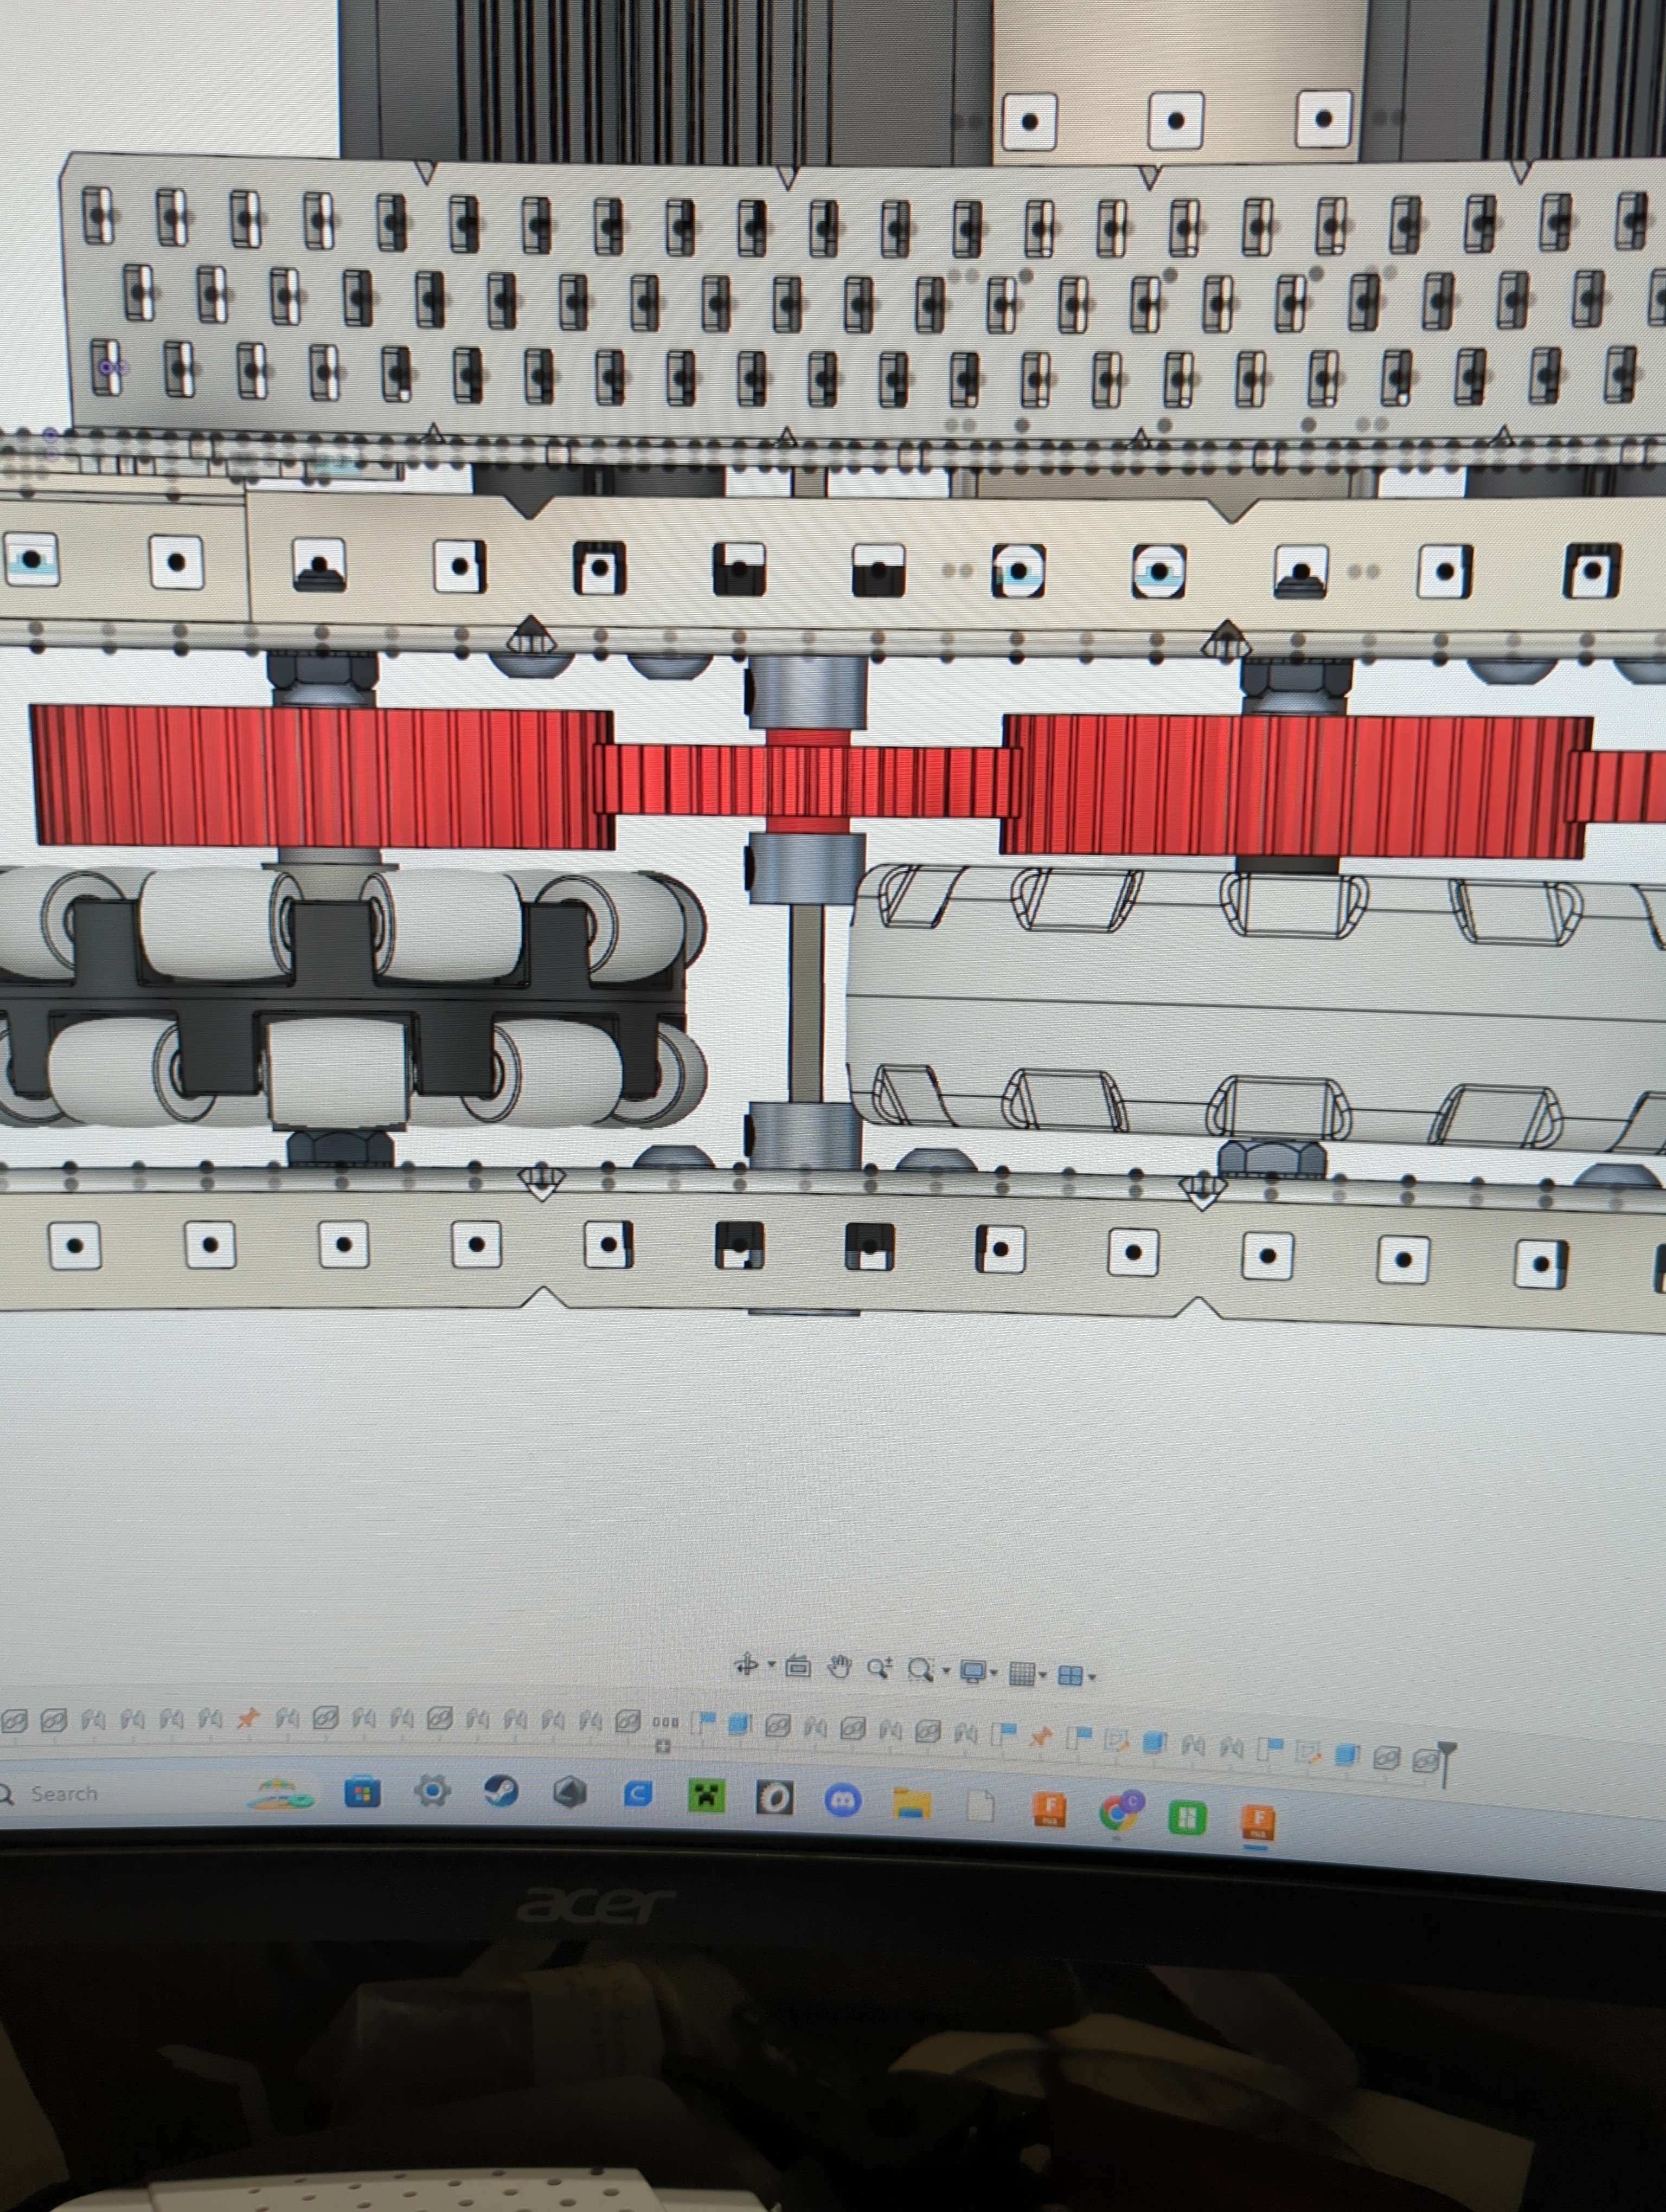
\includegraphics[width=.8\linewidth]{images/450 on 3.25 issue.jpg}
        \caption{450 Rpm Clearance Issue}
        \label{fig:450-on-3.25-issue}
    \end{minipage}
\end{figure}
Ultimately, we settled on a 480 RPM drive with 3.25-inch wheels. This final iteration successfully conformed to our dimensional limit, measuring approximately 14.75" in length, and surpassed our speed requirement with a peak velocity of 82 inches/second. Our wheel arrangement incorporated both, traction and omni wheels in order to overcome the disadvantages of both. by placing a traction wheel in the middle of each side of the drive with omni wheels at the front and rear of it, we overcome the poor turning of the traction wheel by turning it into a pivot and by having a traction wheel at all, we significantly increase our resistance to side pushes. 
\pagebreak
\subsection*{CAD}
Below are the complete CAD designs of our planned drivetrain
\begin{figure}[hbt!] % Use [hbt!] to place the figures on the same page
    \begin{minipage}{.5\textwidth}
        \centering
        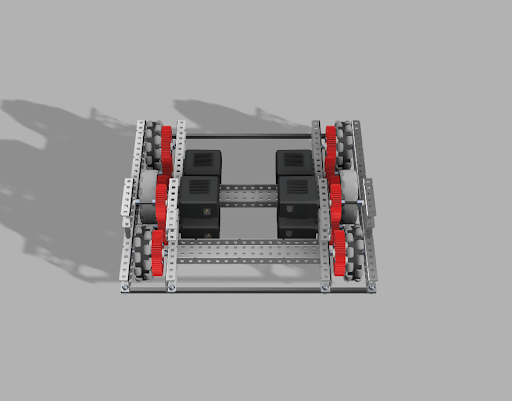
\includegraphics[width=.8\linewidth]{images/Frontdown-V1-Drivetrain.png}
        \caption{Front view}
        \label{fig:frontdown}
    \end{minipage}
    \begin{minipage}{.5\textwidth}
        \centering
        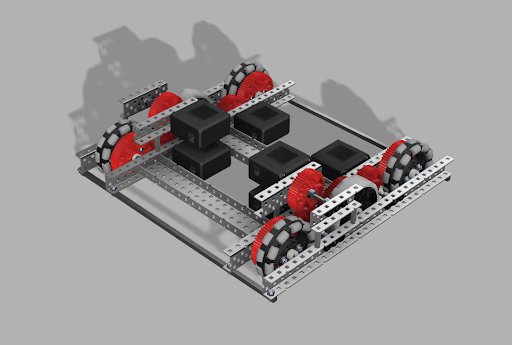
\includegraphics[width=.8\linewidth]{images/Iso-V1-Drivetrain.png}
        \caption{Isometric view}
        \label{fig:iso}
    \end{minipage}
    \begin{minipage}{.5\textwidth}
        \centering
        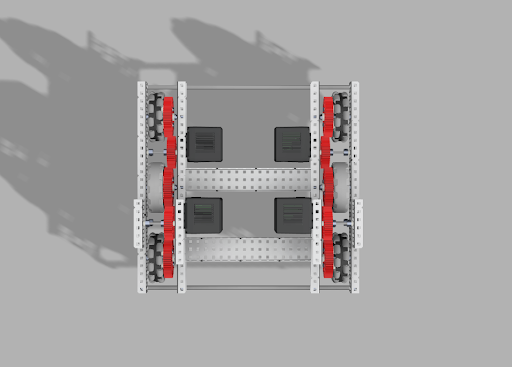
\includegraphics[width=.8\linewidth]{images/Topdown-V1-Drivetrain.png}
        \caption{Top view}
        \label{fig:topdown}
    \end{minipage}
    \begin{minipage}{.5\textwidth}
        \centering
        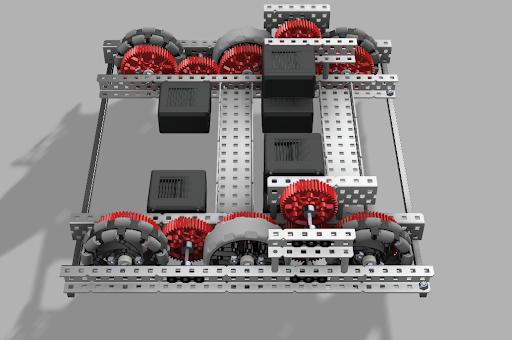
\includegraphics[width=.8\linewidth]{images/Sidedown-V1-Drivetrain.png}
        \caption{Side view}
        \label{fig:sidedown}
    \end{minipage}
\end{figure}

This is our complete CAD for our drivetrain. We always CAD out projects before we build them, so we can see any problems with our potential solution. We decided on 480 RPM using 3.25-inch wheels, measuring approximately 14.75" in length. This will have the velocity of 82 inches/seconds. We see no problems, so we are ready to start building.


\build{Build \& Program: Drivetrain (June 5, 2024)}
\label{Build-&-Program:-Drivetrain}
\chapterauthor{Connor Albers}
\info{Caleb Bachmeier}{Build \& Program: Drivetrain}{June 5, 2024}
\textbf{Goal}: Build \& program our selected drivetrain
    \section*{Building}
\subsection*{Cutting the Drive Rails}
To construct our drive we began by cutting the four "drive rails" to a length of 27 holes; this provided space for our gearing with an extra hole on the front and back of the drive to give room for additional support.
\begin{figure}[h]
    \begin{minipage}{.5\textwidth}
        \centering
        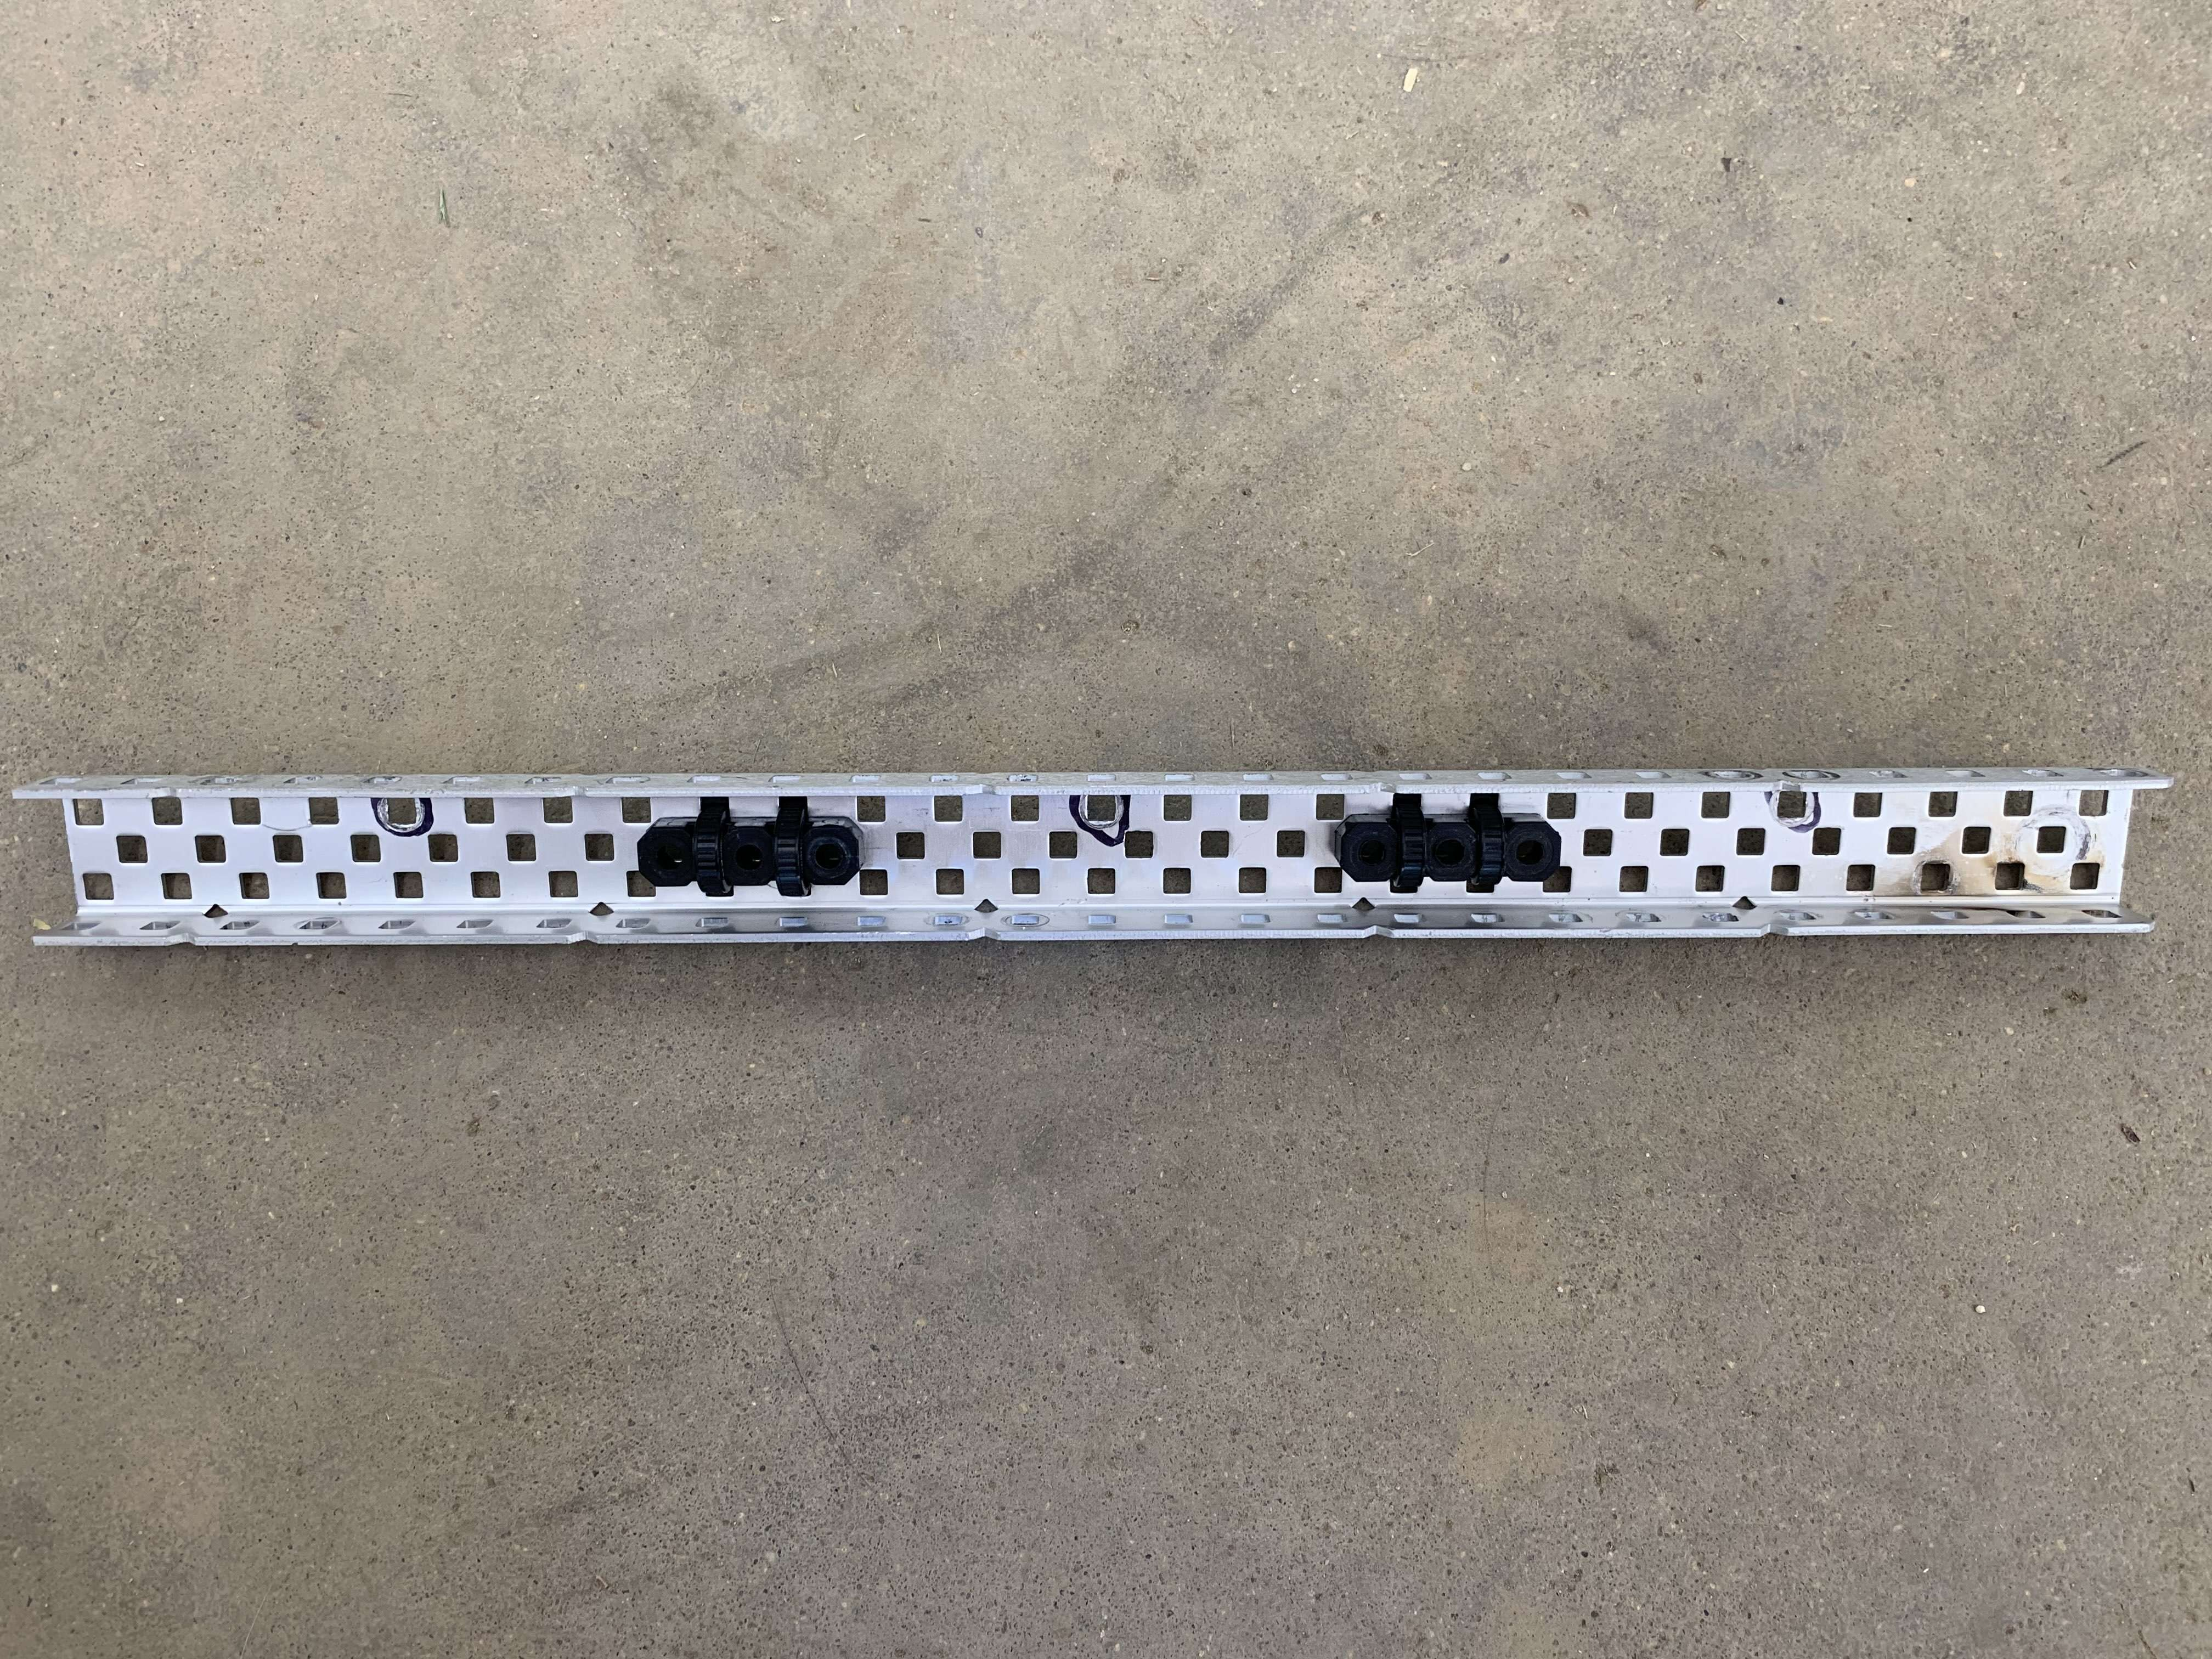
\includegraphics[width=.8\linewidth]{images/C Channel w zipties.jpg}
        \caption{Drive Rail}
        \label{fig:c-chanell-w-zipties}
    \end{minipage}
    \begin{minipage}{.5\textwidth}
        \centering
        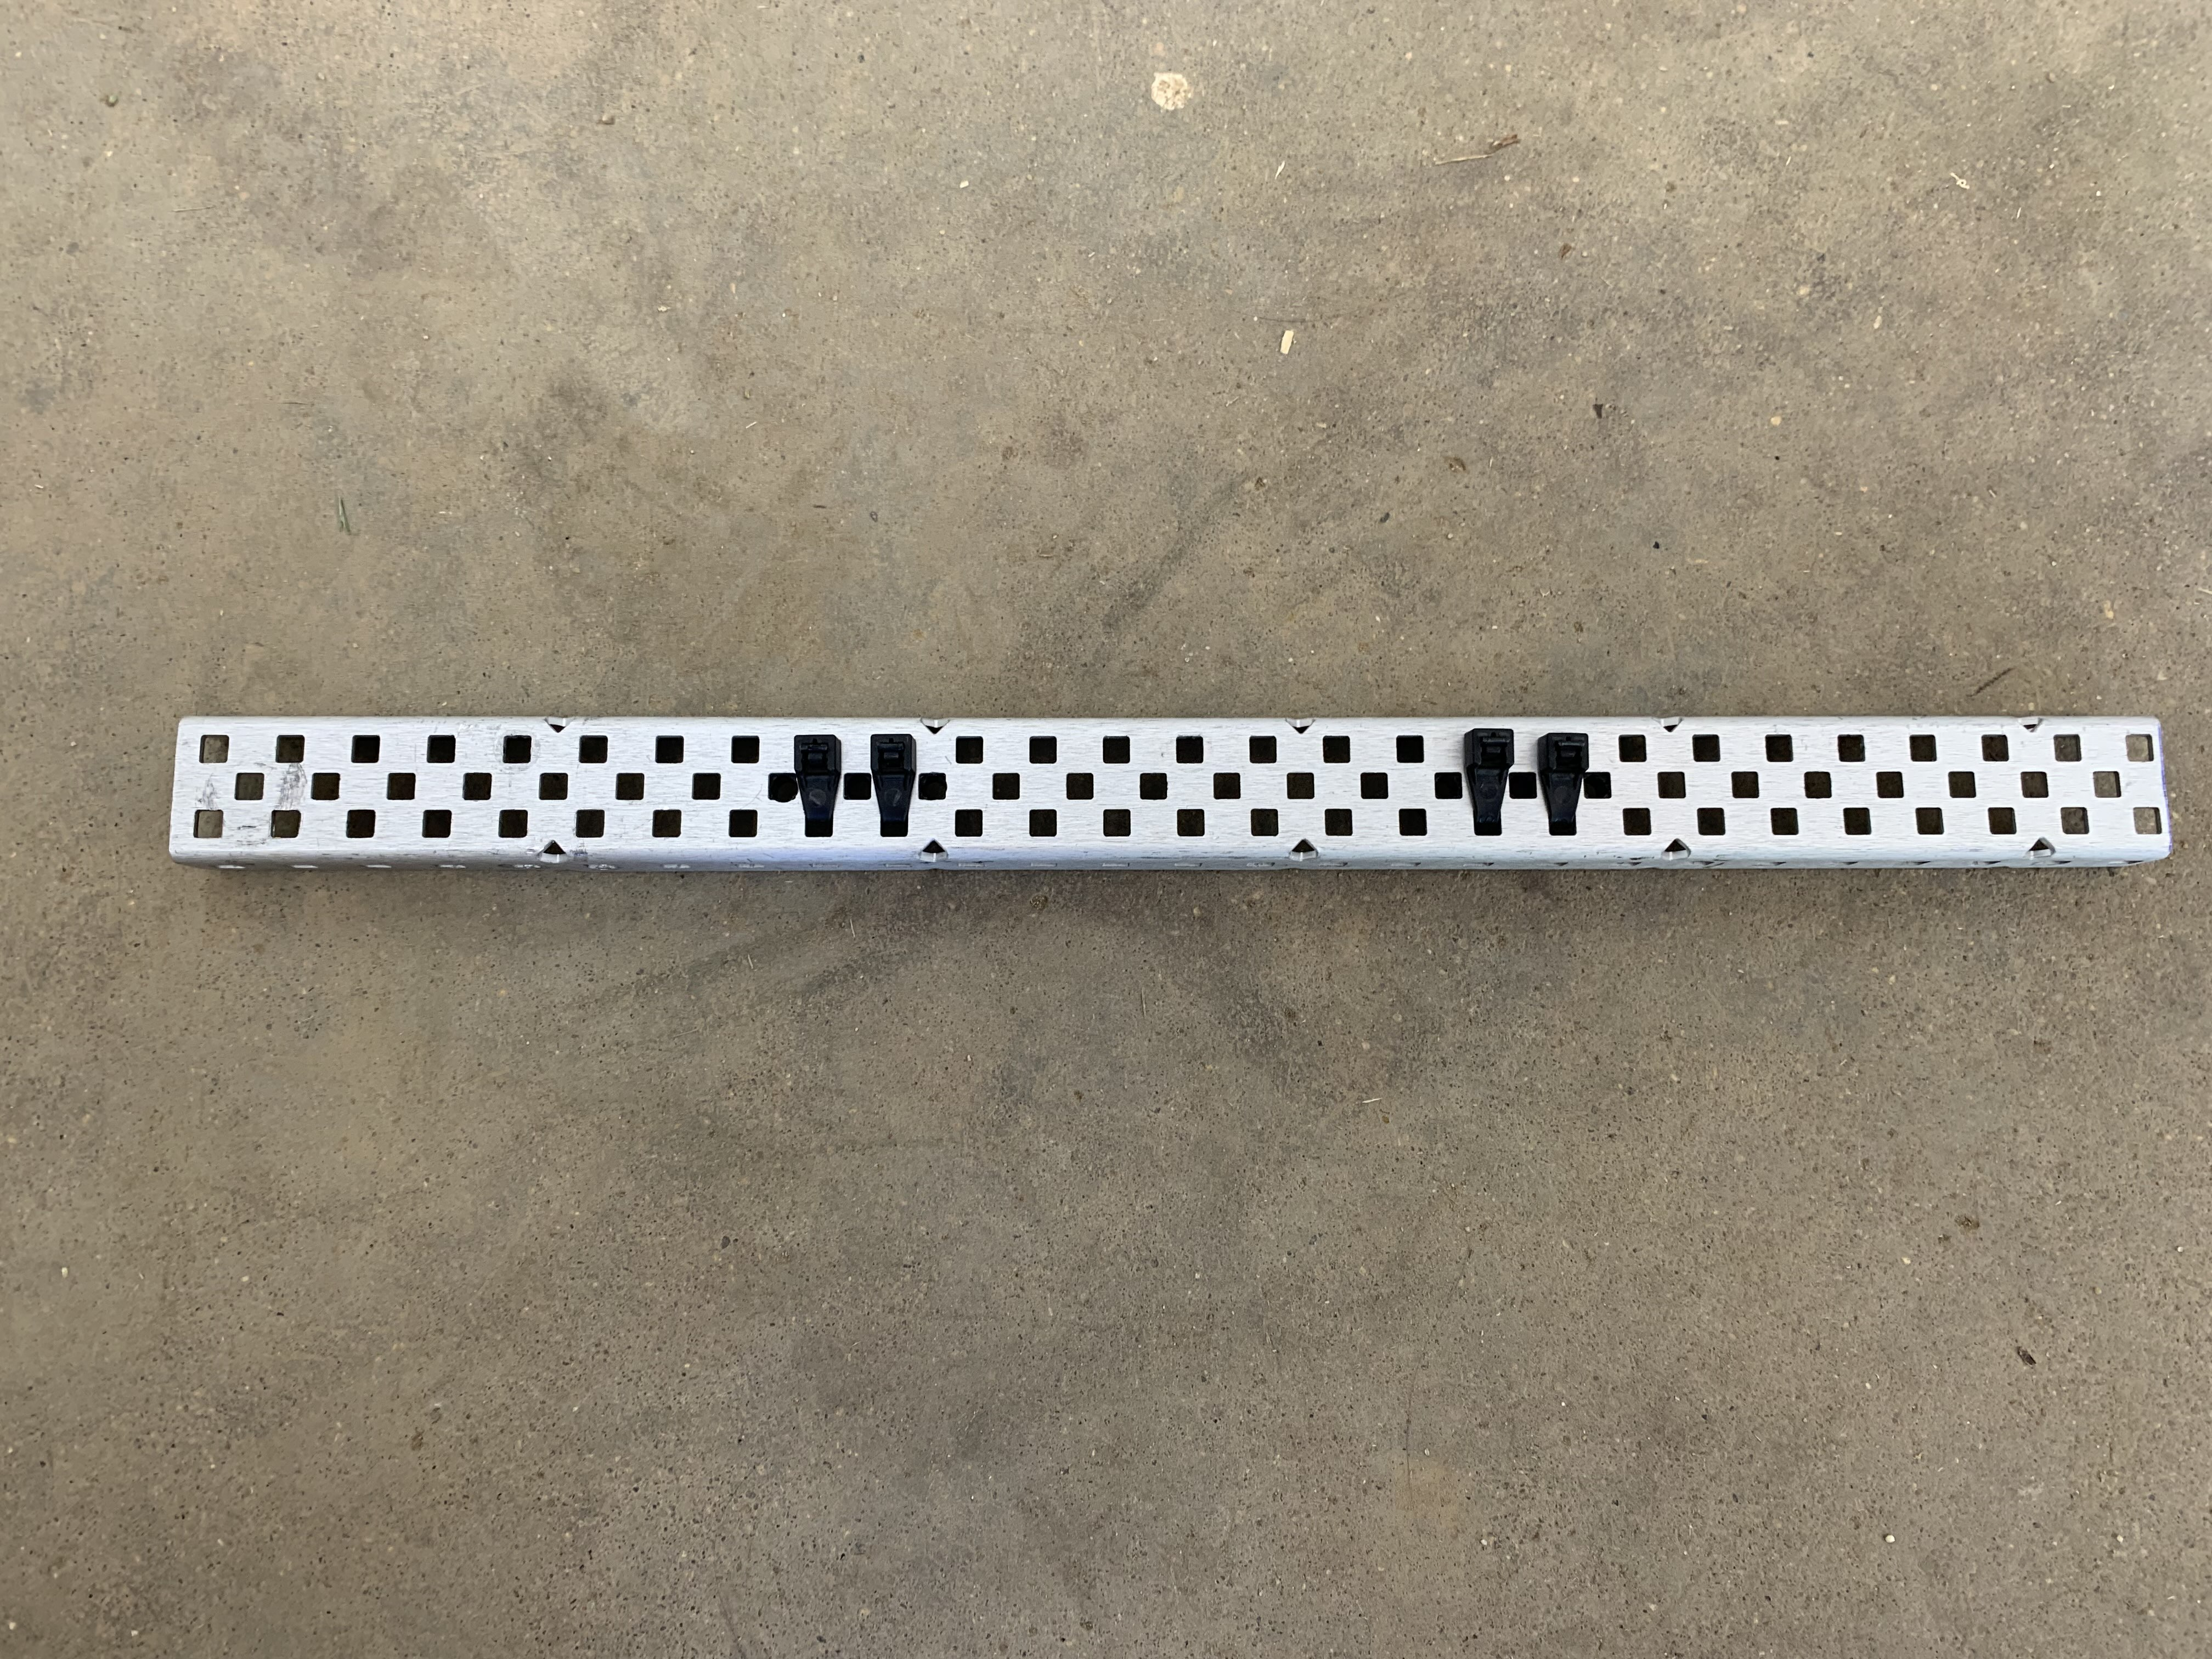
\includegraphics[width=.8\linewidth]{images/Other side of Drive Rail.jpg}
        \caption{Opposite Side of Drive Rail}
        \label{fig:opposite-side-of-drive}
    \end{minipage}
\end{figure}
\subsection*{Zip Tie Bearings}
Our next step was to zip tie the 2 bearings per rail that the idlers gears require. The use of zip tie bearings saves large amounts of weight ultimately contributing to larger acceleration and top speed as well as maneuverability. The bearings are evenly spaced on the the middle row of our 1x2 c-channel drive rails; providing the correct spacing for our gearing.

\subsection*{Adding Screws}
Our next step was to add the 3 screws per side of the drive for the screw joints for the wheels on the bottom row of the drive rails. It is important to note that we inserted the screws into the rails that would end up on the exterior of our drive in order to ensure that we would have access to the screws should we need to tighten any aspect of the joint. After inserting the 2.5" long screws, we threaded lock nuts all the way down the threaded region, effectively turning them into studs. After adding the studs we added 1/4" spacers to all of the studs to prevent the wheels rubbing on the rails; they would rub due to the hubs of the wheels being inset from tread of the wheels.

\subsection*{Constructing Wheel Sub Assemblies and Properly Spacing Them Within the Drive}
Before we could continue the the main build we needed to construct the wheel sub assemblies. While we did have multiple types of wheels, traction and omnidirectional, the process of construction remained the same. The process consisted of using 2 bolts to attach a 60t HS v2 gear to the hub of the wheel with 1/4" spacers in between. Using v2 HS gear removes the need for additional spacers (this is better explained in \blueref{fig:v1-and-v2-gears}{V1 and V2 gears}). After inserting 2 brass circle inserts per wheel, we slid the wheels onto the the screw with the side without the gear facing to what was to be the outside of the drive. Following the wheels, we added 1/8" spacer to each stud; this ensured the spacing between our inside drive rail and outside drive rail was divisible by 1/2"; thus, cohering with the VEX grid system; thence, allowing us to add structure across the drive rails without needing to drill custom holes. The proceeding step was tightening lock nuts on all of the studs to the point where they are as tight as they can be while still allowing the wheels to spin freely. Next we added the second rail to each side followed by a final nut on the end of each study, this time tightening the nut all the way.
\begin{figure}[h!] % Use [hbt!] to place the figures on the same page
        \centering
        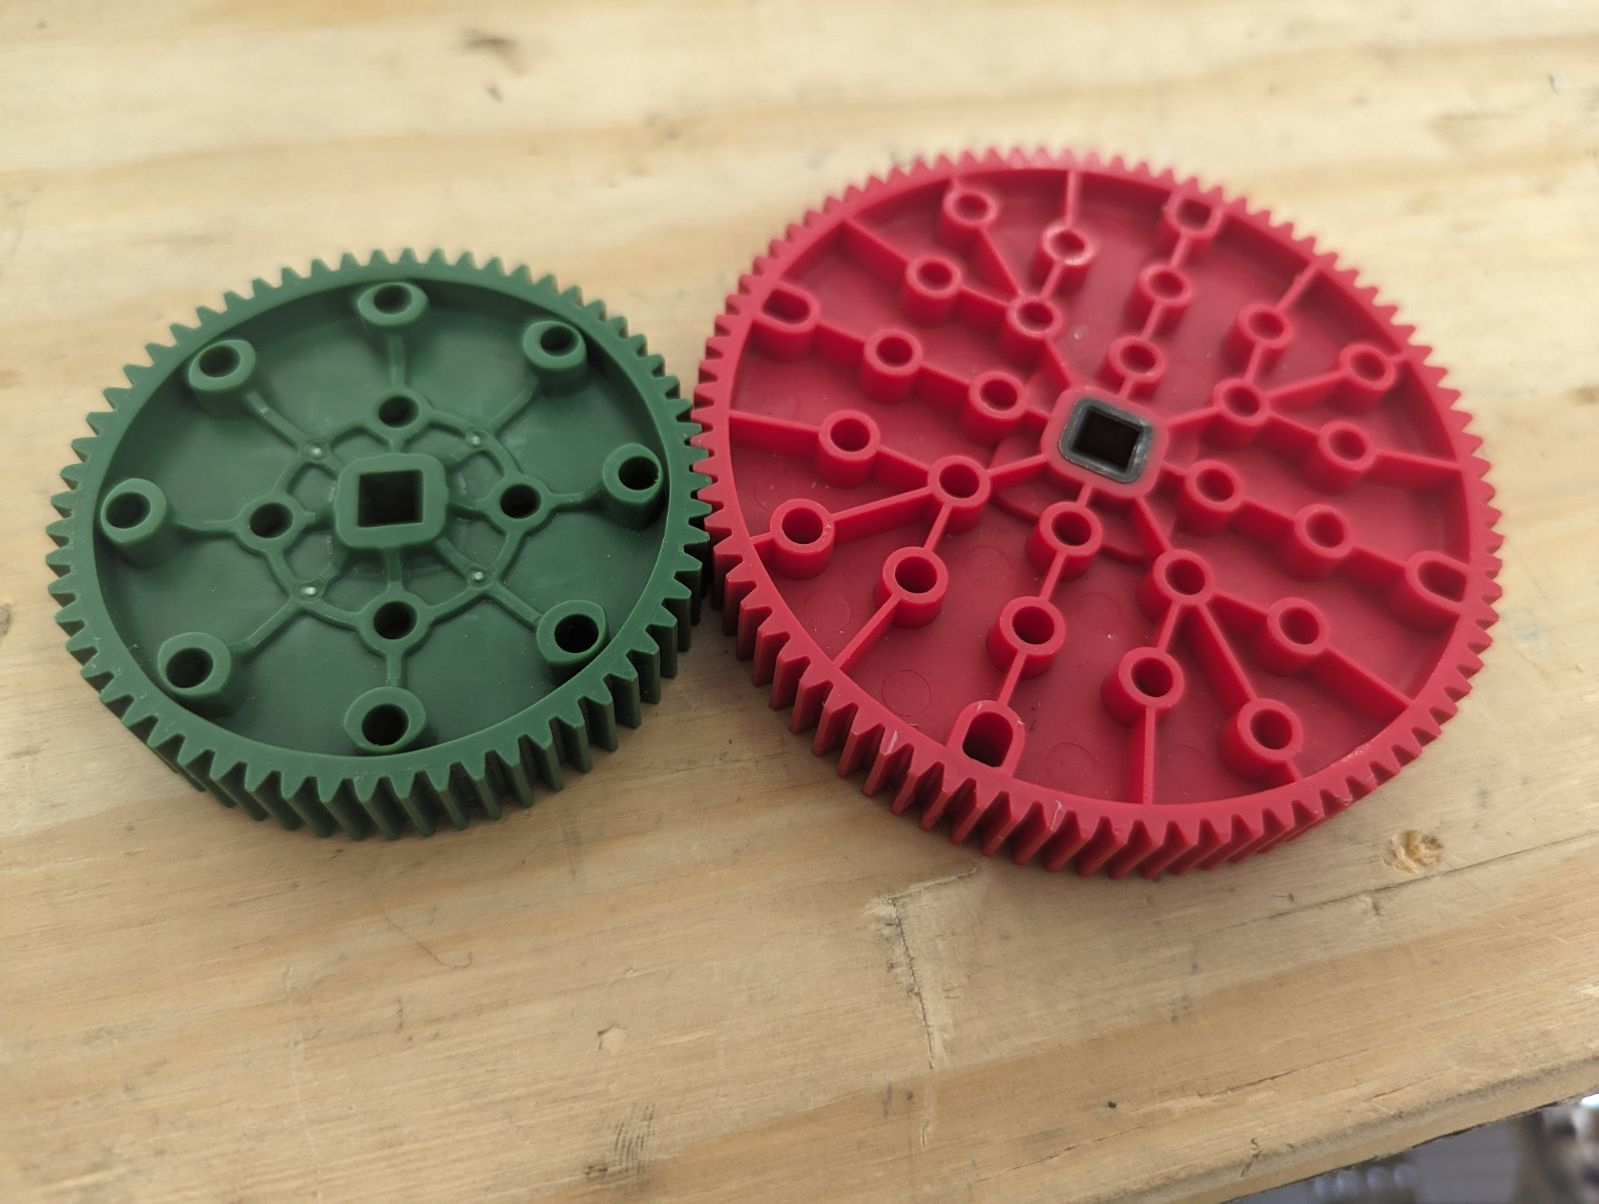
\includegraphics[width=.8\linewidth]{images/V1 and V2 Gears.jpeg}
        \caption{V1 and V2 Gears}
        \label{fig:v1-and-v2-gears}
\end{figure}


\subsection*{Inserting Motor Screws}
The next step was to insert the motor screws as we will not be able to insert them after adding idler gears. This is a very simple step in assembling any VEX component; unfortunately due to spacing issues we were only able to get 1 screw in each motor as opposed the more secure 2. While using only 1 screw per motor is generally not a good idea, we found that by using only 1 screw we can quickly swap motor by inserting our screwdriver through the holes in the outer rail and through the 48t idle gears that are later added.

\subsection*{Adding Idler Gears and Motors}
After cutting 4 shafts to a length of around 3", the next step was to add the shafts for the idler gears, two per side. For specific details on the hardware and spacers used check \blueref{fig:idler-gears}{Idler Gears}. The final step was to add the motors with the addition of steel inserts to ensure the motor gripped the shafts effectively.
\begin{figure}[b]
    \centering
    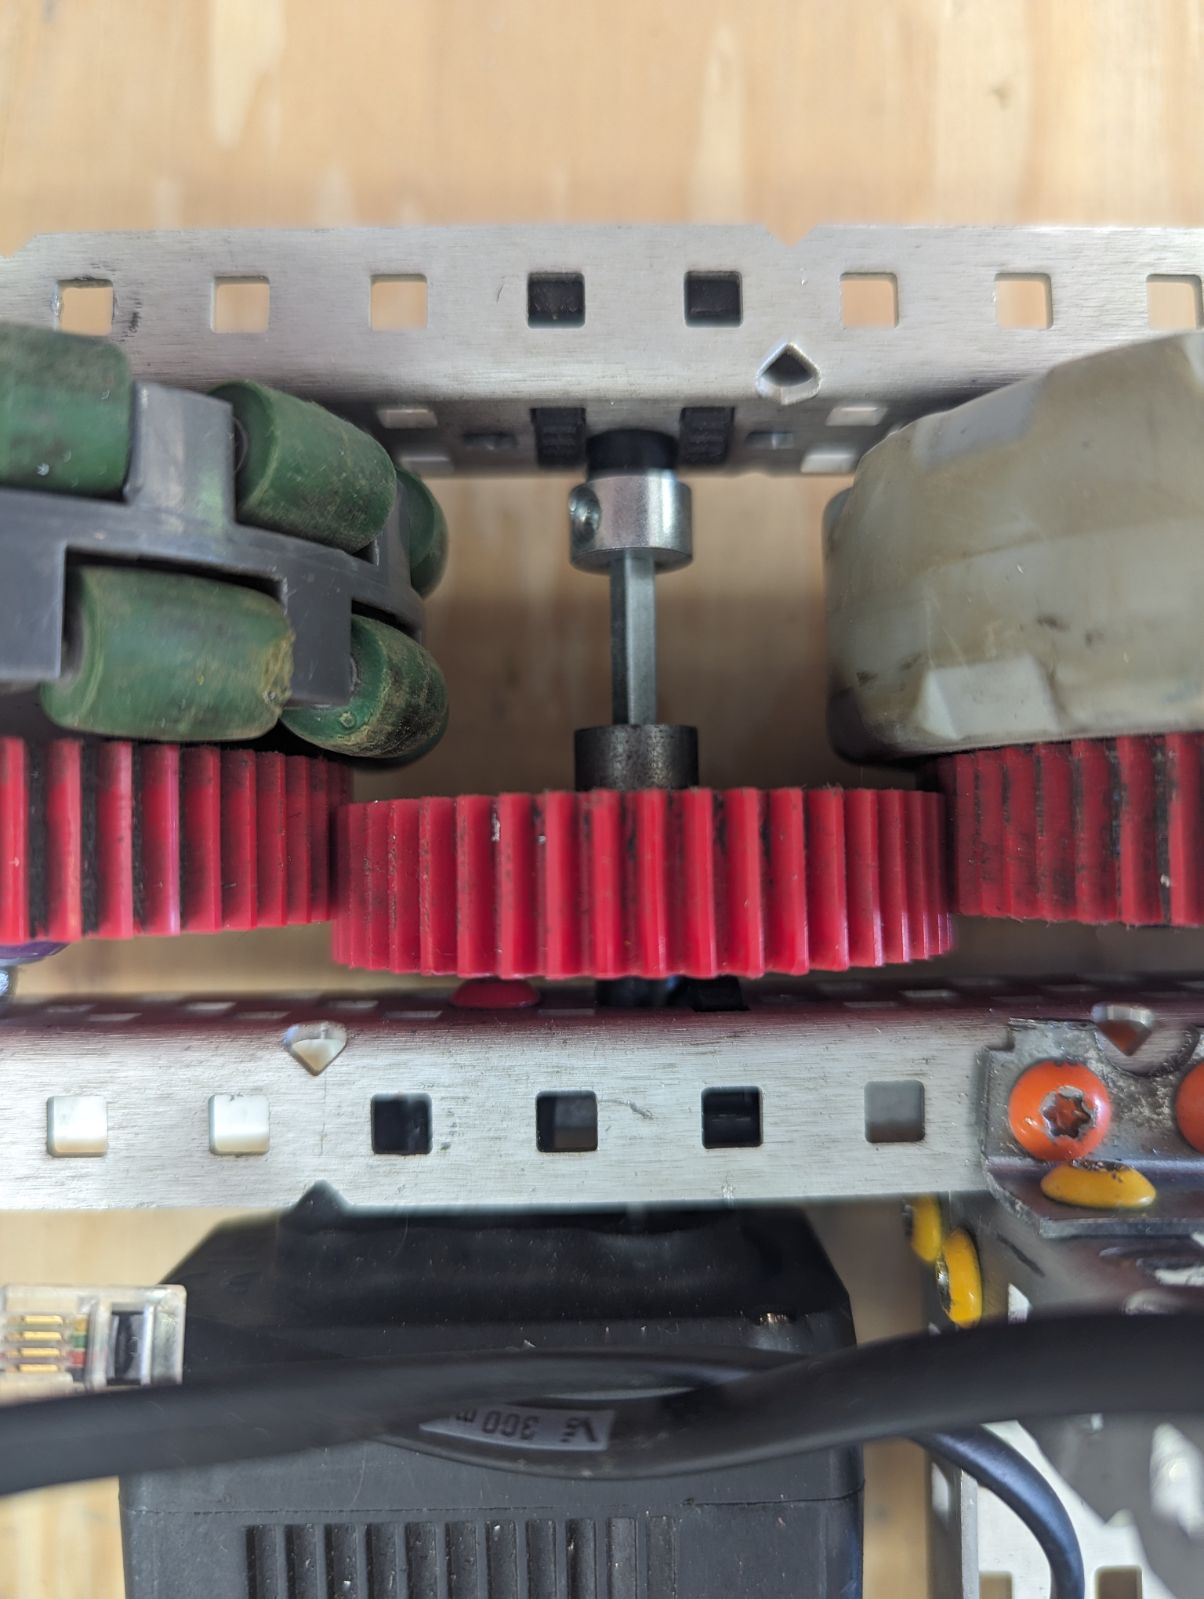
\includegraphics[width=0.5\linewidth]{images/Idler Gears.jpeg}
    \caption{Idler Gears}
    \label{fig:idler-gears}
\end{figure}

\subsection*{Motor Towers}
The current setup only featured a total of four motors but we wanted our final drive to have six. The solution: motor towers. Motor towers are commonly used when a compact motor layout is required or, like in our case, there are too few idle gear axles to add the desired number of motors. Motors towers involve gearing a motor into the drive from above rather that directly into the drive. Our motor towers feature the exact same construction as our idle gears with the only change being that they are moved above the wheels rather than beside them with the help of some 1x5 c-channels that were cut at a length of 5 holes. The use of 1x5 C-Channel provided extra mounting locations should we need them in the future.

\subsection*{Assembling the Drivetrain}
After completing both individual sides of the drive we had to conquer the task of assembling them to be one complete drivetrain. The solution we chose for this was high strength axles. The use of high strength axles provides our drive with copious amounts of strength while remaining low profile so as not to get in the way of other, future mechanisms. Unfortunately using high strength axles, as opposed to c-channel, means we must drill out every point we wish to attach to. This was simply unpractical for anything beyond attaching the sides of the drivetrain together. Our approach to this problem included using high strength axles that spanned the entire width of the drive and using shorter c-channels that only spanned to the inter lip of each side of the drive. This is better explained in \blueref{fig:mounting-rails-hs-axles}{Mounting rails with high strength axles}. After mounting just 1 high strength axle at both the front and rear of the drive, our drive turned out to be surprisingly rigid -- being the most rigid drive we had ever built.
\begin{figure}[h]
    \centering
    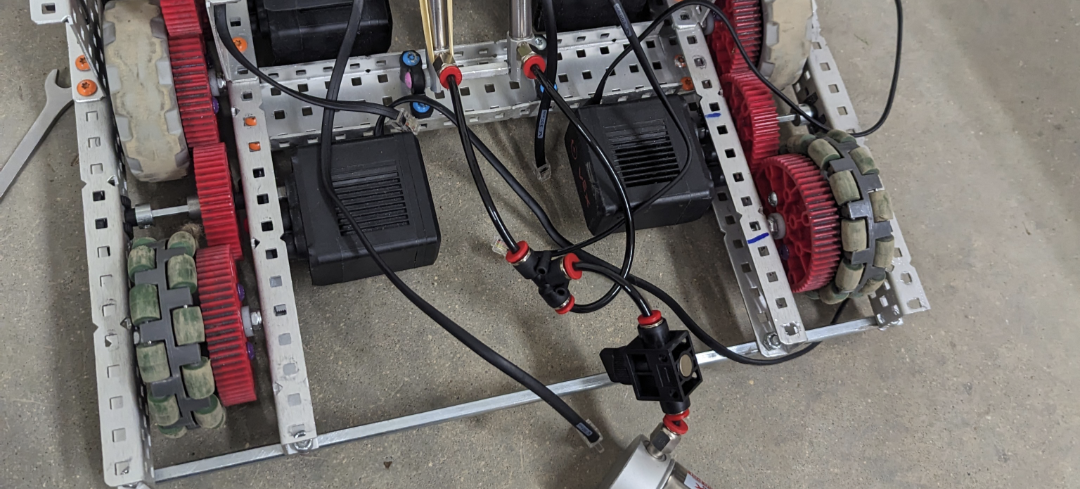
\includegraphics[width=1\linewidth]{images/Mounting Rails HS Axles.png}
    \caption{Mounting the Rail}
    \label{fig:mounting-rails-hs-axles}
\end{figure}
\begin{figure} [hbt!]
    \begin{minipage}{.5\textwidth}
        \centering
        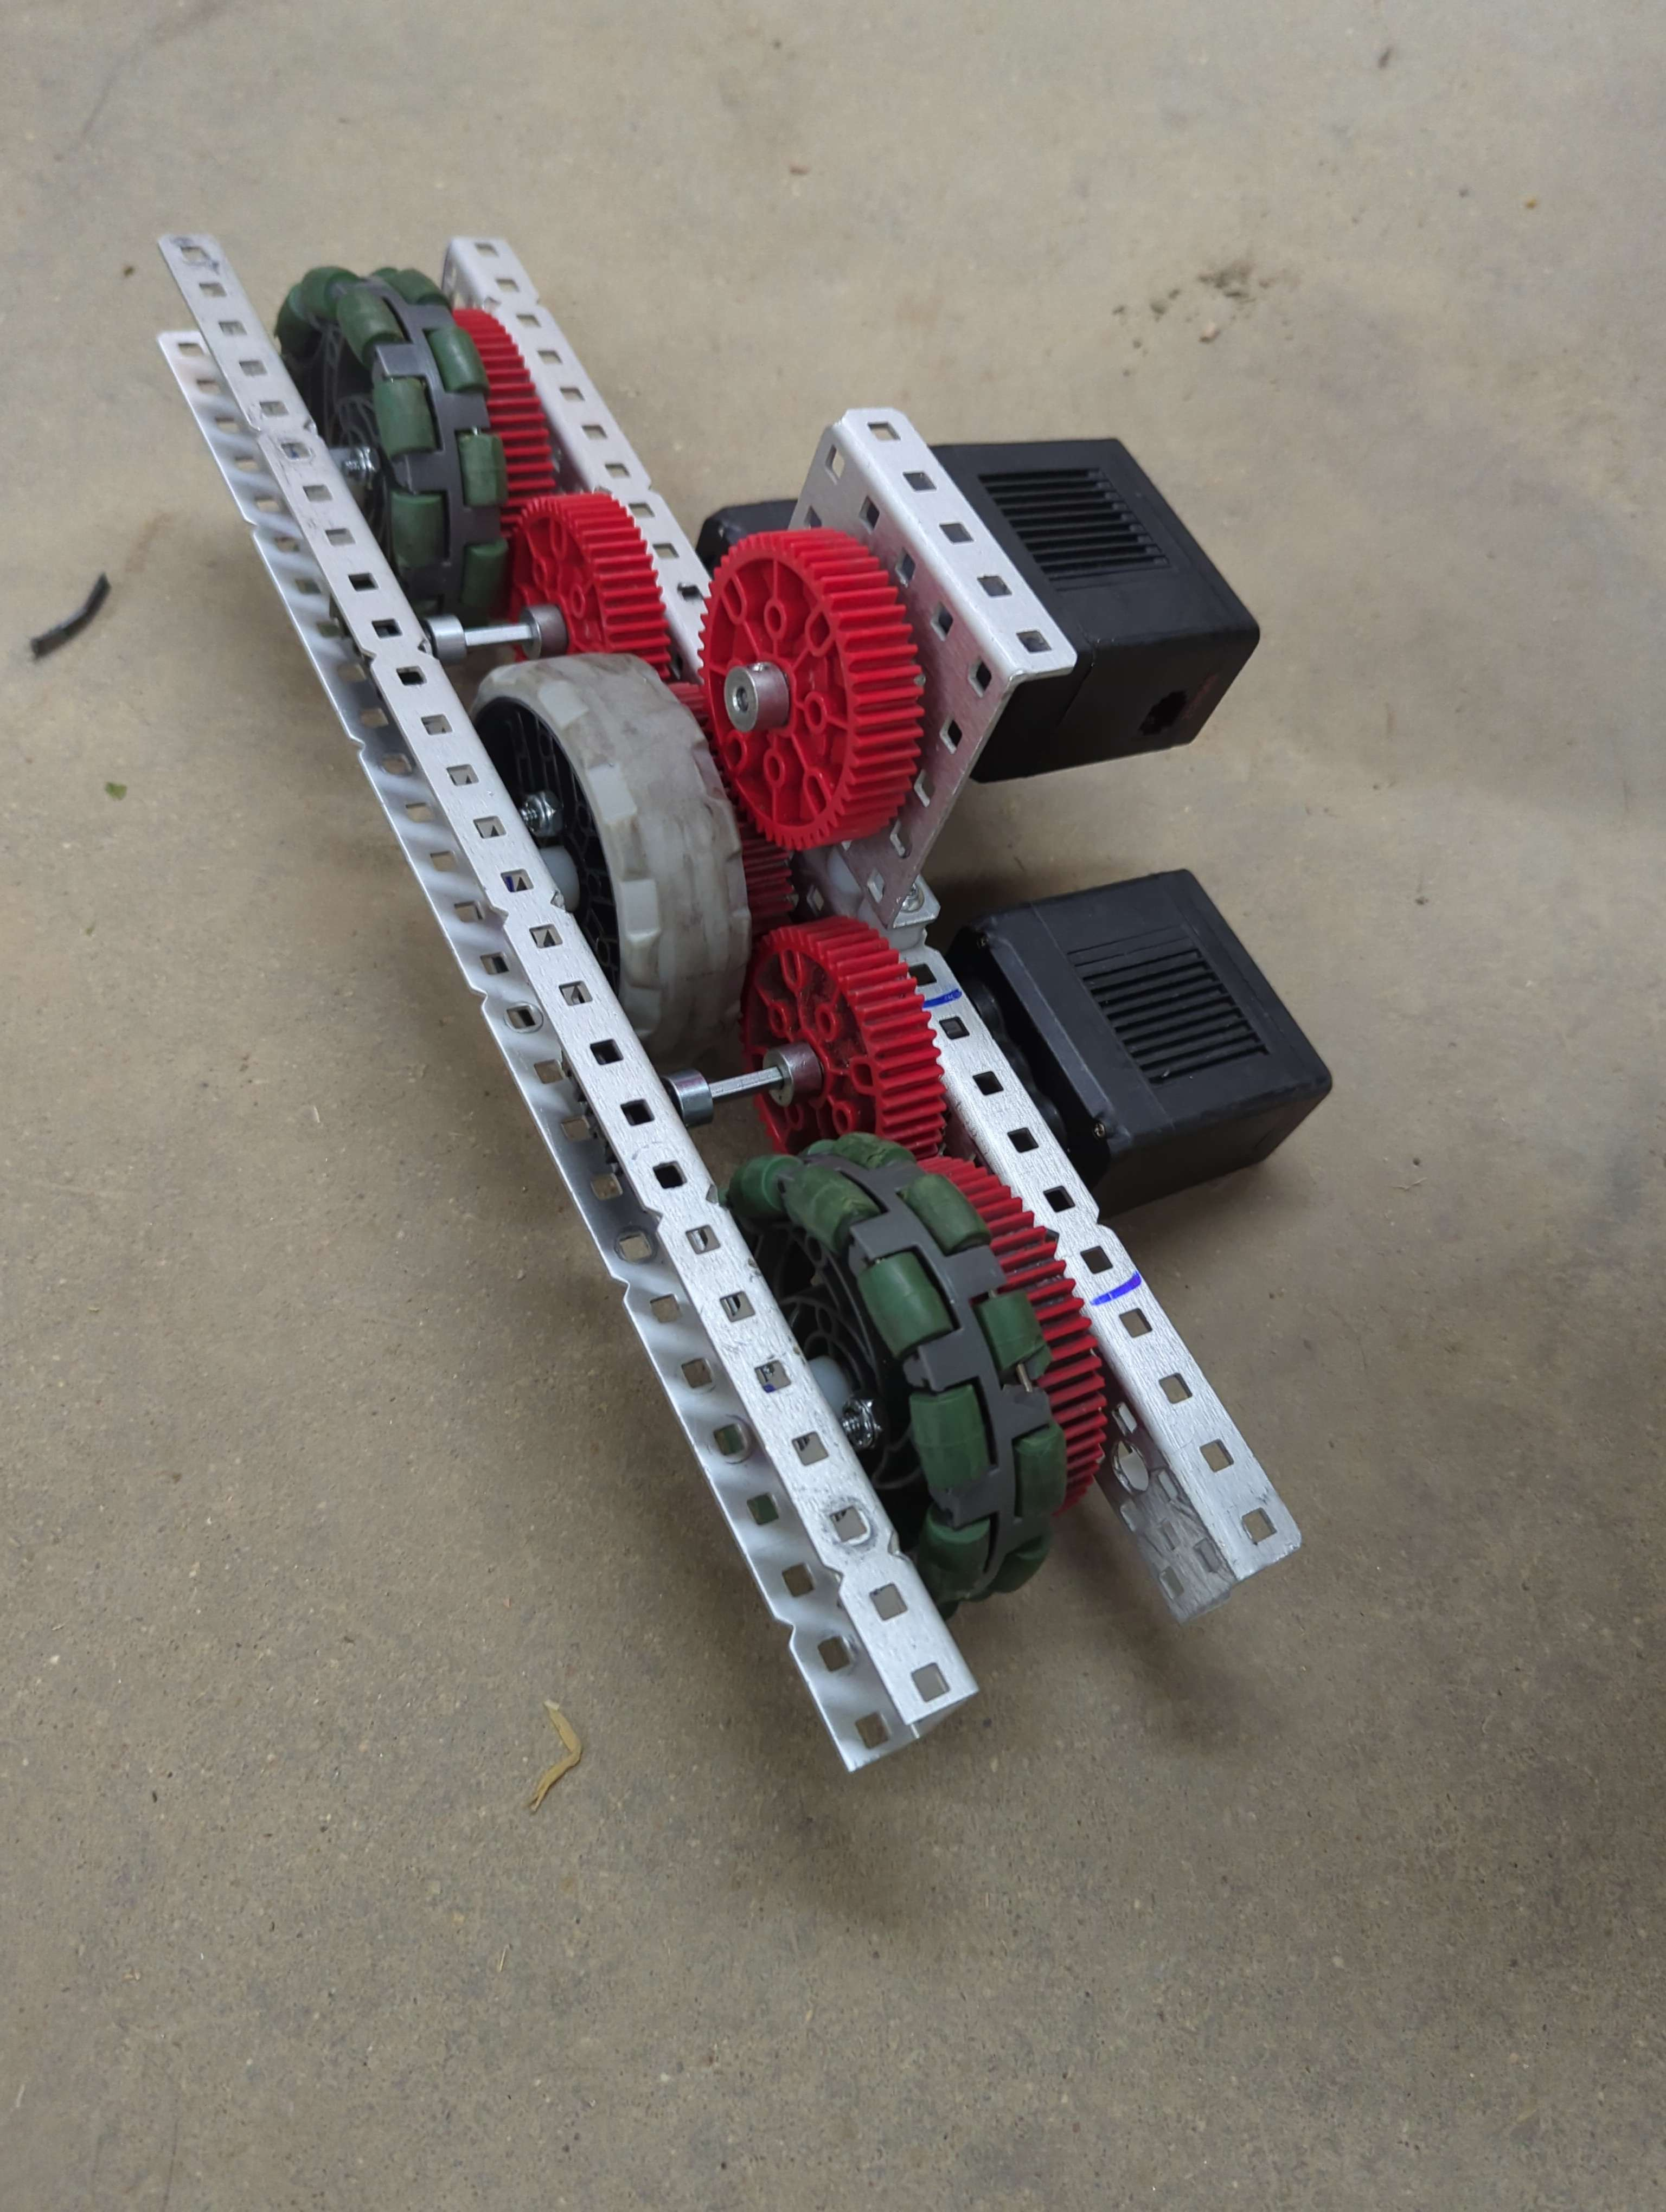
\includegraphics[width=.8\linewidth]{images/Full Drive.jpg}
        \caption{Single Side of Drive}
        \label{fig:side-of-drive}
    \end{minipage}
     \begin{minipage}{.5\textwidth}
        \centering
        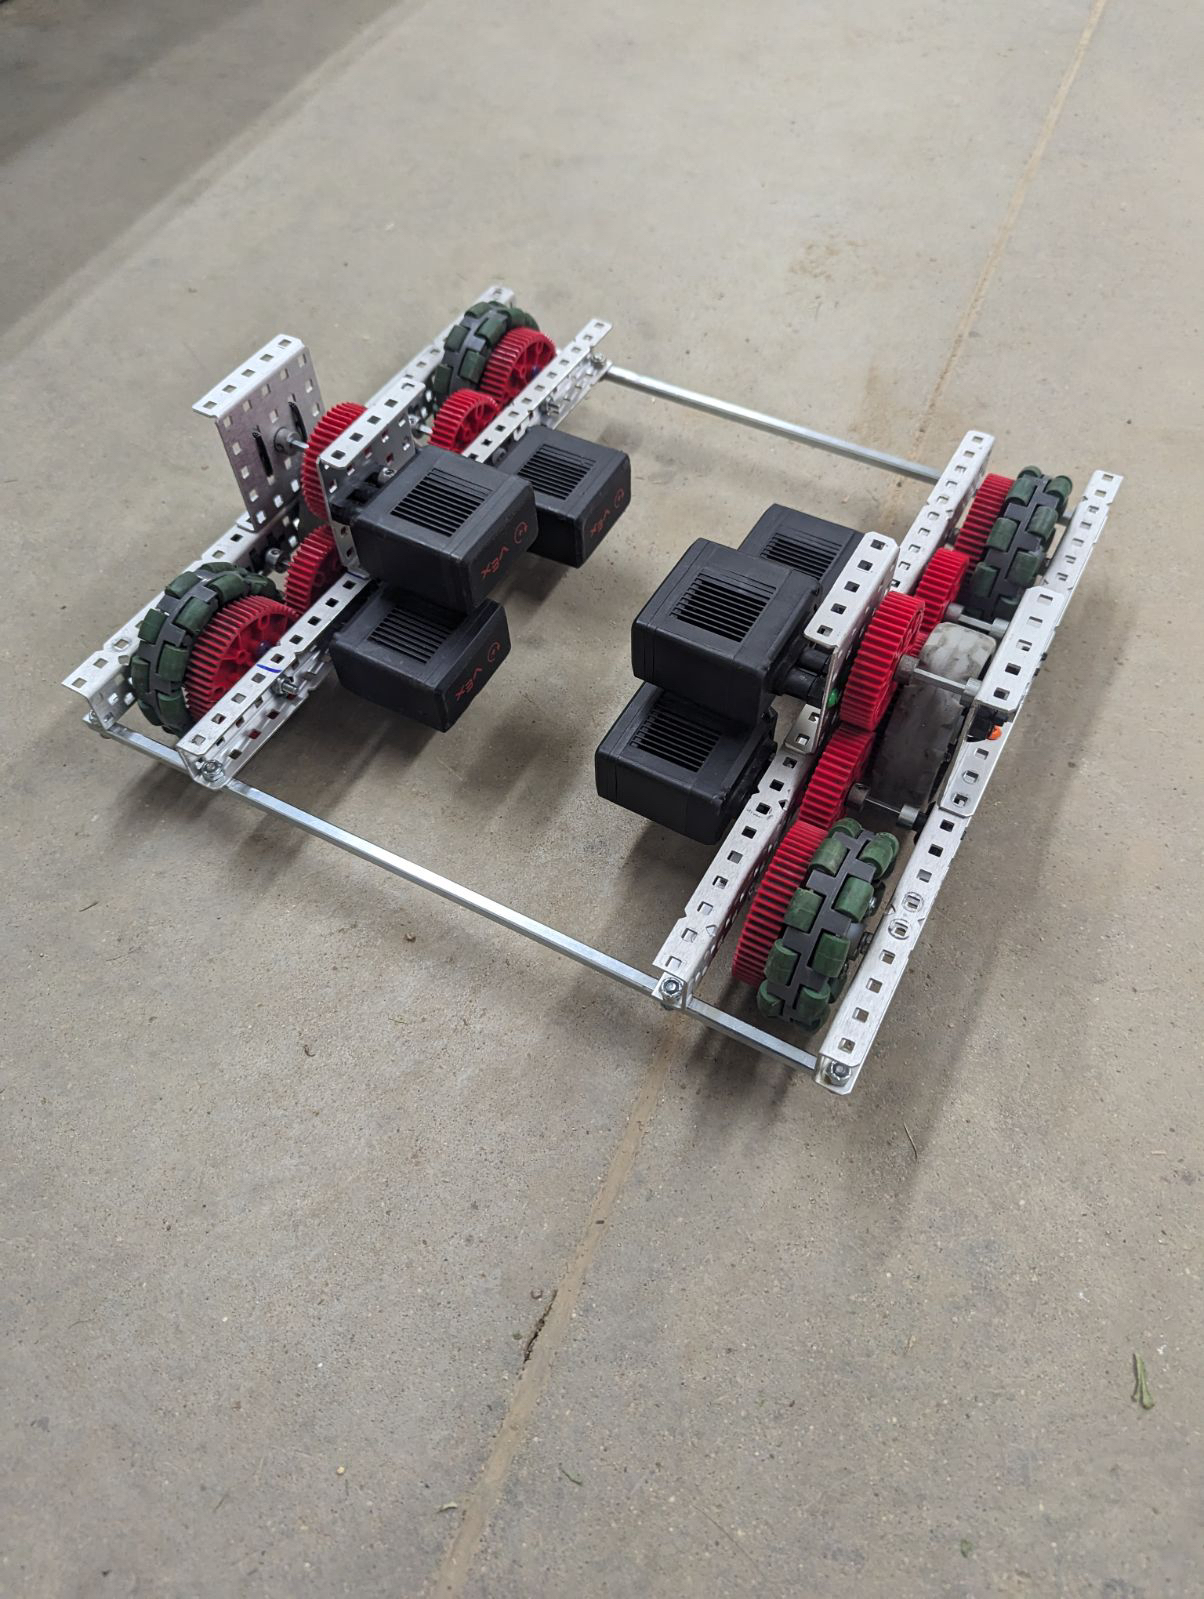
\includegraphics[width=.8\linewidth]{images/Drivetrain.jpg}
        \caption{Drivetrain}
        \label{fig:drivetrain}
    \end{minipage}
\end{figure}
\test{Test the Solution (June 8, 2024)}
\label{Test-the-Solution}
\chapterauthor{Caleb Bachmeier, Ian Smith}
\info{Caleb Bachmeier}{Test the Solution}{June 8, 2024}
\textbf{Goal}: Test our built drivetrain
    \section*{Test the Solution}
After temporarily mounting our brain, battery and radio to the robot, we coded it to drive using speed curves and curvature drive. Both of these are better explained in the next paragraph. By coding our drive in the same way it will be coded at competitions, we can let our drivers get a feel for the robot -- it is worth noting that this 'feel' with change as we add additional mechanisms to the robot. We still need to do some testing on our robot to ensure that our speed is correct, the equation to find our theoretical speed is:
\[
t = \frac{d}{v}
\]
Where
\begin{itemize}
    \item t is the time (in seconds),
    \item d is the distance (in inches), and
    \item v is the speed of the robot (in inches per second).
\end{itemize}
Using this data we will add in our expected result into the table below:

For 5 feet (60 inches):
\[
t = \frac{60}{82} \approx 0.73 \, \text{seconds}
\]

For 10 feet (120 inches):
\[
t = \frac{120}{82} \approx 1.46 \, \text{seconds}
\]

For 20 feet (240 inches):
\[
t = \frac{240}{82} \approx 2.93 \, \text{seconds}
\]

The formula for percent error is:

\[
\text{Percent Error} = \left( \frac{|\text{Experimental Value} - \text{Theoretical Value}|}{\text{Theoretical Value}} \right) \times 100
\]

\textbf{Variables}
\begin{itemize}
    \item Independent: length
    \item Dependant: time
    \item Constant Factors: 
    \begin{itemize}
        \item Same robot
        \item Floor were are testing on (The foam tiles on the VEX VRC field)
        \item Stopwatch
        \item Environment (Inside)
    \end{itemize}
\end{itemize}


\renewcommand{\arraystretch}{1.85} % Change this value as needed
\begin{table}[htb!]
\centering
\begin{tabular}{|>{\centering\arraybackslash}m{1.85cm}|>{\centering\arraybackslash}m{1.85cm}|>{\centering\arraybackslash}m{1.85cm}|>{\centering\arraybackslash}m{1.85cm}|>{\centering\arraybackslash}m{1.85cm}|>{\centering\arraybackslash}m{1.85cm}|>{\centering\arraybackslash}m{1.85cm}|}
\hline
\textbf{} & \textbf{5 Feet} & \textbf{10 Feet} & \textbf{20 Feet}
\tabularnewline
\hline
Expected Result & 0.73 seconds & 1.46 seconds & 2.93 seconds \tabularnewline
\hline
Actual Result & 0.84 seconds & 1.65 seconds & 2.95 seconds \tabularnewline
\hline
Difference & 0.11 seconds & 0.19 seconds & 0.02 seconds \tabularnewline
\hline
Percent Error & 15.07\% & 13.02\% &  0.68\% \tabularnewline
\hline
\end{tabular}
\caption{Drive Testing}
\end{table}
\renewcommand{\arraystretch}{1.85} % Reset to default
\pagebreak
\section*{Speed Curves and LemLib}

Below is a paragraph written by \blueref{Ian}{Ian Smith} on the Advantages of Speed and Steer Curves when driving:

\vspace{1cm}

The concept of a speed curve is used when discussing driver assists. At the most fundamental level, speed curves are used to allow the driver to have more precise control at lower joystick positions while sacrificing control at higher motor velocities. The reason this is advantageous is because a lower motor velocity is synonymous with requirements of finer driver control. Thus, more space on the joystick is given for areas at lower velocity where the drive may want to be more precise. This takes just a little bit of the fine motor control skill away from the driver itself and compensates mathematically. Originally when writing my first motor curve function, I originally used a switch.case argument using only linear functions. The next adaptation was an exponential curve using the base \(e\). However, the latest adaptation of motor curves was after using the LemLib library, where the motor curve functions were already built into the drivetrain class, saving me time having to modify some code. This forum has been a help in the later implementation of motor curves in combination with LemLib due to the nature of the way constants are layed out 

\href{https://www.vexforum.com/t/expo-drive-lemlibs-implementation/123337}{This is a link to VEX Forums about LemLib's Implementation into VRC}. \href{https://www.desmos.com/calculator/umicbymbnl}{Here is the interactive Desmos page developed by the LemLib team.}
 %June 8
\identify{Identify the Challenge \& Set Goals: MoGo Mechanism (June 15, 2024)}
\label{Identify-the-Challenge-&-Set-Goals:-Clamp}
\chapterauthor{Caleb Bachmeier}
\info{Caleb Bachmeier}{Identify the Challenge \& Set Goals: MoGo}{June 15, 2024}
\textbf{Goal}: We will identify an objective for our robot so that we can address it and build an effective way to pickup stakes
\section*{Problem Statement}
\texthl{We must create a mechanism that effective picks stakes up, so that we can put rings on them.}
\section*{Solution Requirements}
\begin{itemize}
    \item Must only use legal VEX VRC parts
    \item Must fit in the 18" x 18" x 18" cube
    \item Must be able to fit on our drivetrain 
    \item Must use no more than 44 watts (four, eleven watt motors). 
    \item Another, often overlooked, problem is the scarcity of parts, parts are not unlimited. Because of problems at our regular practice place (the place with all of our parts) we must practice elsewhere. Not being able to access  parts is a huge problem.
\end{itemize}
\section*{Solution Goals}
\begin{itemize}
    \item We would love to use pneumatics, so we can use our 22 remaining watts elsewhere.
\end{itemize}
\brainstorm{Brainstorm \& Diagram: MoGo Mechanism (June 17, 2024)}
\label{Brainstorm-&-Diagram:-Clamp}
\chapterauthor{Caleb Bachmeier}
\info{Caleb Bachmeier}{Brainstorm \& Diagram: MoGo}{June 17, 2024}
\textbf{Goal}: Brainstorm our clamp ideas and diagram them
\section*{Possible Solution - MoGo Mechanism}
\noindent
\textbf{Clamp}:

\noindent
\textbf{Pros}:
\begin{itemize}
    \item We would be able use pneumatics 
    \item Very simple design
    \item Very reliable
\end{itemize}
\textbf{Cons}:
\begin{itemize}
    \item If we do use pneumatics, we would have to set up a whole pneumatic system 
    \item It can be complicated to use leverage to clamp the stake down
    \item A clamp would require maintenance 
\end{itemize}

\noindent
\textbf{Forklift}:

\noindent
\textbf{Pros}:
\begin{itemize}
    \item Forklifts can be simpler to design and build compared to complex clamping mechanisms.
    \item A forklift allows you to adjust the height at which you pick up and place rings on the stake. This flexibility can be advantageous for scoring at different levels.
    \item Depending on how you build it, Forklifts typically have a smaller footprint than clamps, leaving more room for other mechanisms on your robot.
\end{itemize}
\textbf{Cons}:
\begin{itemize}
    \item  Ensuring stability while lifting and placing rings can be challenging. The stake may sway or wobble during the process.
    \item Forklifts add weight to the robot, potentially affecting overall performance.
    \item Accurate alignment is crucial for successful ring placement using a forklift.
    \item We could use pneumatics, although it would negate the largest potential benefits.
\end{itemize}
\noindent
\textbf{Scissor Lift}:

\noindent
\textbf{Pros}:
\begin{itemize}
    \item Scissor lifts can extend to various heights, allowing you to reach different levels of the stake.
    \item When compressed, scissor lifts tend to be more stable, making them reliable for lifting rings from lower positions.
    \item Scissor lifts occupy less space compared to some other mechanisms.
\end{itemize}
\textbf{Cons}:
\begin{itemize}
    \item Scissor lifts can be heavy, affecting overall robot performance. Ensuring stability at higher extensions can be challenging.
    \item As the lift extends, it requires more torque to lift the load. This can impact motor efficiency.
    \item Building a stable scissor lift with precise alignment can be intricate.
\end{itemize}

\solution{Choose a Solution \& Make a Plan: MoGo Mechanism (June 23, 2024)}
\label{Choose-a-Solution:-Clamp}
\chapterauthor{Caleb Bachmeier}
\info{Caleb Bachmeier}{Choose a Solution \& Make a Plan: MoGo}{June 23, 2024}
\textbf{Goal}: Choose which solution we will use for our clamp
\section*{Choose a Solution}
\renewcommand{\arraystretch}{1.85} % Change this value as needed
\begin{table}[htb!]
\centering
\begin{tabular}{|>{\centering\arraybackslash}m{1.85cm}|>{\centering\arraybackslash}m{1.85cm}|>{\centering\arraybackslash}m{1.85cm}|>{\centering\arraybackslash}m{1.85cm}|>{\centering\arraybackslash}m{1.85cm}|>{\centering\arraybackslash}m{1.85cm}|>{\centering\arraybackslash}m{1.85cm}|}
\hline
\textbf{Scale 1 - 10} & \textbf{Stability} & \textbf{Simplicity} & \textbf{Cost} & \textbf{Durability} & \textbf{Total} \tabularnewline
\hline
Weight & x3 & x1 & x1 & x2 & \tabularnewline
\hline
Clamp & 10 & 5 & 9 & 10 & 64 \tabularnewline
\hline
Forklift & 6 & 6 & 5 & 6 & 41 \tabularnewline
\hline
Scissor Lift & 6 & 8 & 4 & 4 & 38 \tabularnewline
\hline
\end{tabular}
\caption{Clamp Decision Matrix}
\label{tab:clamp-matrix}
\end{table}
\renewcommand{\arraystretch}{1.85} % Reset to default
Looking at our point totals it would seem that a clamp design would work best for our purpose.
\subsection*{CAD}
\begin{figure}[h!] % Use [hbt!] to place the figures on the same page
    \begin{minipage}{.55\textwidth}
        \centering
        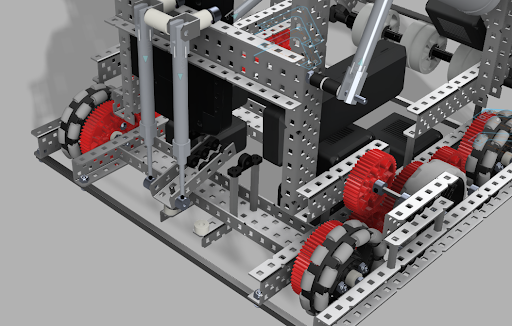
\includegraphics[width=1\linewidth]{images/Iso-Clamp-V1.png}
        \caption{Isometric View}
        \label{fig:iso}
    \end{minipage}
    \begin{minipage}{.55\textwidth}
        \centering
        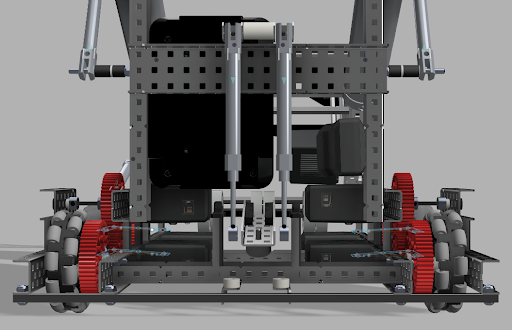
\includegraphics[width=1\linewidth]{images/Front-Clamp-V1.png}
        \caption{Front View}
        \label{fig:front}
    \end{minipage}
    \begin{minipage}{.55\textwidth}
        \centering
        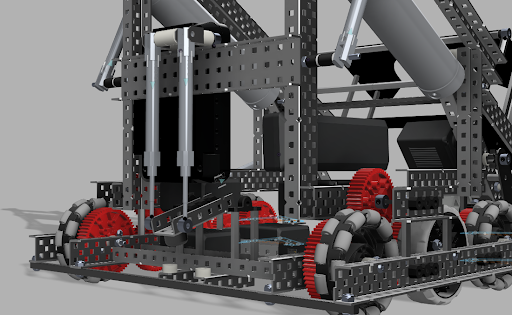
\includegraphics[width=1\linewidth]{images/Side-Clamp-V1.png}
        \caption{Side View}
        \label{fig:side}
    \end{minipage}
    \begin{minipage}{.55\textwidth}
        \centering
        \includegraphics[width=1\linewidth]{images/Bottom-Clamp-V1.png}
        \caption{Bottom View}
        \label{fig:bottom}
    \end{minipage}
\end{figure}

On the following page there are four CAD images describing how we would like to build our clamp. It would use two 55mm stroke double action pistons to push down on the mobile goal and hold it in place. Now it's time to build.
\build{Build: MoGo Mechanism (June 25, 2024)}
\label{Build-&-Program:-Clamp}
\chapterauthor{Caleb Bachmeier}
\info{Caleb Bachmeier}{Build: MoGo}{June 25, 2024}
\textbf{Goal}: Build \& program our selected solution
\section*{Building}
\section*{Initial Concept and Prototype}
One of the first things we did after constructing our drivetrain was design a mobile goal clamp that would allow us to move and score on mobile stakes. Our first design, inspired by our sister team, 7686A, used 2 pistons to pivot C-channels, pressing down and securing a mobile goal. 

Although we designed the concept in CAD before building it, the motion limits within the piston in CAD were far shorter than those on the actual piston. This meant we had to redesign the clamp to work with shorter pistons. Since this was our first prototype and we were eager to see it working, we added spacers to adjust where the pneumatics pivoted on the clamp lever. This version looked rather awkward, but it functioned as expected.

\section*{Reducing Footprint and Design Iteration}
During the construction of our scoring mechanisms, we realized that the current clamp design interfered with the clearance needed by several mechanisms. To reduce the clamp’s footprint, we swapped the original 75mm pistons with 50mm ones, which allowed us to remove the previously added spacers. This provided the necessary clearance for our initial scoring mechanism iterations. However, when we began constructing our first hook intake, we identified the need for further redesign.

\section*{Second-Class Lever Design}
Our new design featured a second-class lever, where the pistons were mounted on the same end that contacted and clamped the mobile goals. We continued using 50mm pistons, but instead of attaching them to the drivetrain base, we mounted them on our intake tower, above the clamp. (See Figure~\ref{fig:lever-design}.) 

Mounting the pistons in this way kept them clear of the inside of the drivetrain, ensuring enough space for the intake chain to pass through. This adjustment significantly improved the integration of our clamp with the rest of the robot.

\section*{Adding Stoppers for Distance and Angle Control}
A major part of our clamp’s functionality was adding stoppers to control how far the mobile goal could enter our robot and at what angle it would sit once clamped. Managing the entry distance was crucial since it determined the clamp’s contact point, directly affecting the grip on the goal. Through testing and incrementally increasing the size of the stoppers on either side of the goal, we found that high-strength shaft collars worked perfectly.

\section*{Angle Control and Hooking Mechanism}
We also needed to control the mobile goal's angle, as it impacted the proximity of the goal’s top to the intake chain. With feedback from 7686A, we determined that the optimal distance was around 2 inches, where the intake hooks would just barely graze the silicone cap when spinning by.

To implement this, we mounted two L-channels just below the clamp’s pivot point. We added a cut low-profile bearing and a spacer, along with a screw, onto each L-channel. This spacer and screw acted as a hook that caught the bottom lip of the mobile goal, preventing it from being removed by opposing teams.

\begin{figure}[h]
    \centering
    \includegraphics[width=0.8\textwidth]{images/Clamp Lever.jpeg}
    \caption{Second-Class Lever Clamp Design with 50mm Pistons.}
    \label{fig:lever-design}
\end{figure}

\test{Test the Solution: MoGo Mechanism (June 25, 2024)}
\label{Test-the-Solution:-Clamp}
\chapterauthor{Caleb Bachmeier}
\info{Caleb Bachmeier}{Test the Solution: MoGo}{June 25, 2024}
\textbf{Goal}: Test our built solution 
\section*{Test the Solution}
Our clamp has been built and now ready to test, but how should we test it? We thought about using a Spring Scale to measure the force of our pistons, but we already know the force of them; one of our pistons has twelve pounds of force which is approximately 53.4 Newtons of total force, so two pistons would be approximately 106.8 N of force. Then we thought about the force of the Mobile Goal and Rings on the pistons. A Ring weighs 4.3 oz or 122 g. One mobile goal weighs 33.44 oz or 948 g.

So \[1_\text{Ring} \approx 1.196 N\] \[1_\text{Mobile Goal} \approx 9.297 N\] \[2_\text{Pistons} \approx 106.8 N\]

It was then we realized: \[106.8N \text{(The force of our clamp)} > 16.437N\text{(The force of one mobile goal and six rings)}\]

If the force of our clamp was always greater than the force of anything we would need to lift, we wouldn't need the entire 106.8 N of our pneumatics would offer, so as long as our clamp is good enough to lift 16.437 N of force, we should be good.
\section*{Test}
Our test for the clamp is very simple, at which angles could a mobile goal be clamped from? This may sound like an odd question, but it is a very real issue for some teams. This is shown in the image below \\
\begin{figure}[h!]
    \centering
    \includegraphics[width=0.5\linewidth]{images/MoGo w Highlights.jpeg}
    \caption{MoGo Issues}
    \label{fig:mogohighlights}
\end{figure}
Some teams have problems clamping onto the mobile goal at these highlighted areas. We need to see if this is a problem for us. \blueref{fig:clamp-v1-corner-test}{(This testing is continued on the next page)}

Another test we need to do is to find the angles at which each mobile goal is clamped down on. We wanted to do this to make sure their weren't any oddities in our data. We used a digital angle finder.
Our data is as follows:
\[
1 \; \text{Mobile Goal} \; + 0 \; \text{Ring} = 7.6 \degree
\]
\[
1 \; \text{Mobile Goal} \; + 1 \; \text{Ring} = 7.6 \degree
\]
\[
1 \; \text{Mobile Goal} \; + 2 \; \text{Ring} = 7.5 \degree
\]
\[
1 \; \text{Mobile Goal} \; + 3 \; \text{Ring} = 7.3 \degree
\]
\[
1 \; \text{Mobile Goal} \; + 4 \; \text{Ring} = 7.2 \degree
\]
\[
1 \; \text{Mobile Goal} \; + 5 \; \text{Ring} = 7.0 \degree
\]
\[
1 \; \text{Mobile Goal} \; + 6 \; \text{Ring} = 6.9 \degree
\]

Our data seems very consistent ranging from 7.6 \degree - 6.9 \degree. This concludes our testing for the clamp, it seems that it was a very good decision and has high build quality. Now time to build our intake mechanism.

\pagebreak

\begin{figure}[h!] % Use [hbt!] to place the figures on the same page
    \begin{minipage}{.5\textwidth}
        \centering
        \includegraphics[width=.8\linewidth]{images/Clamp Test V1.jpg}
        \caption{Clamp V1 Test}
        \label{fig:clamp-v1-test}
    \end{minipage}
    \begin{minipage}{.5\textwidth}
        \centering
        \includegraphics[width=.8\linewidth]{images/Clamp Corner Test V1.jpg}
        \caption{Clamp V1 Corner Test}
        \label{fig:clamp-v1-corner-test}
    \end{minipage}
    \begin{minipage}{.5\textwidth}
        \centering
        \includegraphics[width=.8\linewidth]{images/Clamp Corner Test V1.1.jpg}
        \caption{Clamp V1 Corner Test}
        \label{fig:clamp-v1.1-corner-test}
    \end{minipage}
\end{figure}

These are the tests for our built Clamp, as you can see, in \blueref{fig:clamp-v1-corner-test}{these photos} our test to figure out if we can clamp from the corners is successful. This concludes our testing for the Clamp, it seems to be a very efficient solution for a MoGo mechanism.  %June 25
\important{Update to Judging - June 25th}
\chapterauthor{Caleb Bachmeier}
\textbf{Goal}: Breakdown Version 1.0 of V5RC High Stakes Game Manual
\section*{Update to Judging}

On June 25th, 2024, Version 1.0 of the V5RC High Stakes Game Manual was released. This was an extreme update, of which this chapter will break down.
\subsection*{Field Layout}
\textit{Changed the Field layout such that Positive Corners and Negative Corners are now on the same side of the field} 

This is a change that will not affect the strategy. I believe this was a change to make the field symmetrical 
\subsection*{Rule Changes}
\textit{Added a new rule, SC9, that adds a 2-point bonus for whichever Alliance has a ring Scored on the High Stake at the end of the match} 

This was a needed bonus to incentivize scoring a ring on the top stake. Before it was not worth it.  

\textit{Rewrote SG5c to clarify that preloads cannot start in a scored location} 

This update was also necessary to change. I'm happy they discovered this loophole before the season began 

\textit{Added a new rule, SG11, to add a 10 second protection to Positive Corners at the end of the match} 

This is a very controversial update, but yet another to motivate people to hang. The fights over the positive corners would be very interesting, but I believe these updates will still happen, but over the negative corners rather than the positive corners.
\white{July 2024}
\begin{center}
    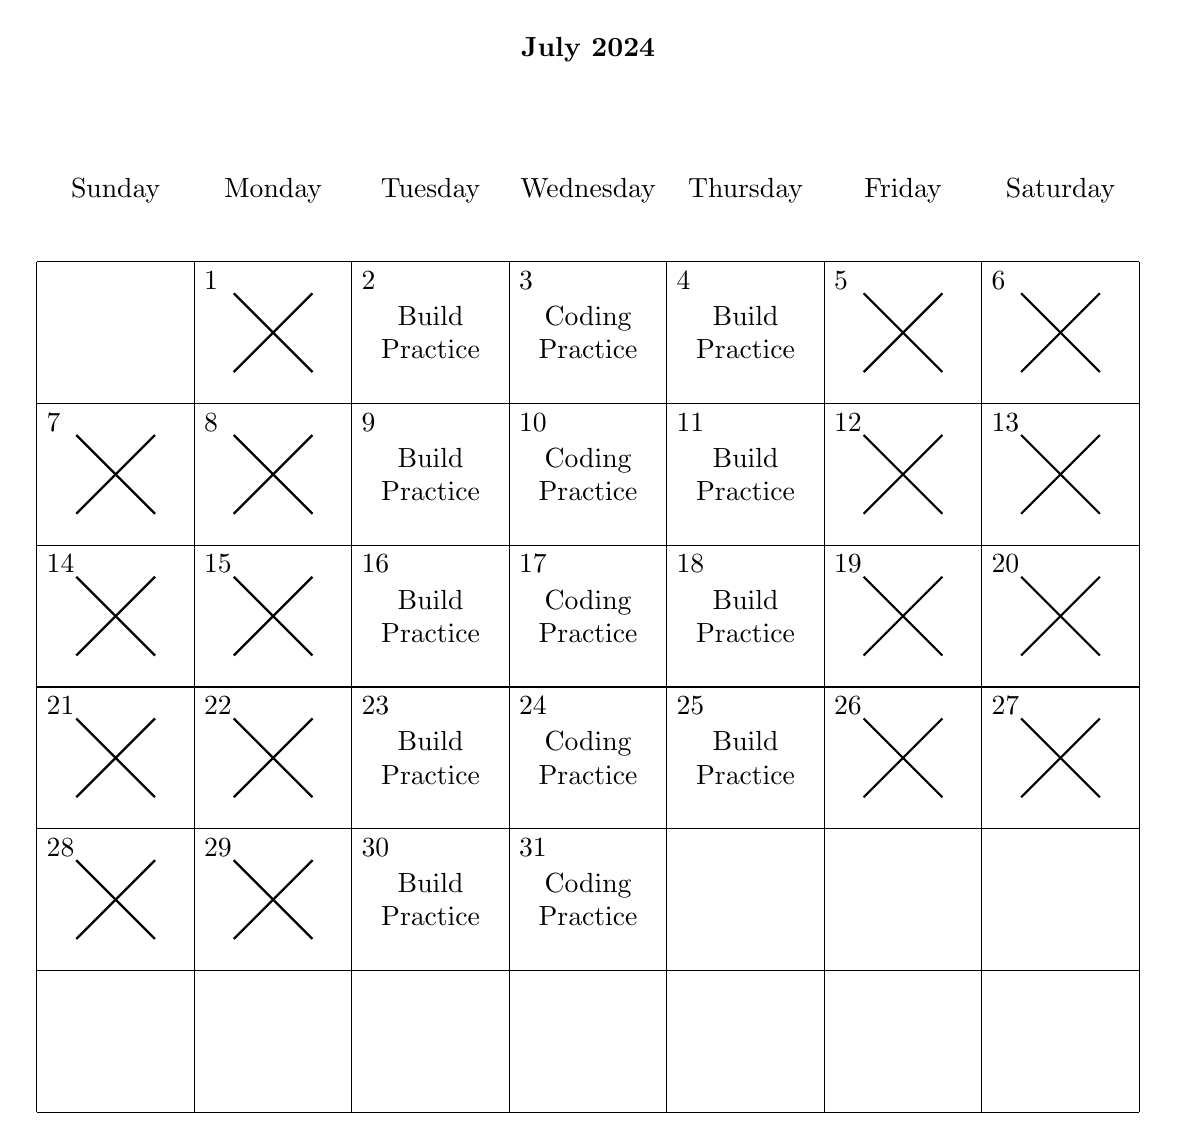
\begin{tikzpicture}
        % Define the dimensions of the calendar
        \def\year{2024}
        \def\month{7}
        \def\monthname{July}
        \def\startday{2} % 1=Sunday, 2=Monday, ..., 7=Saturday
        \def\numdays{31}
        \def\boxwidth{2} % Width of each box
        \def\boxheight{1.8} % Height of each box

\newcommand{\daytext}[1]{
    \ifcase#1
    \or \cross \or Build Practice  \or Coding Practice \or Build Practice \or \cross \or \cross \or \cross \or \cross \or Build Practice \or Coding Practice
    \or Build Practice \or \cross \or \cross \or  \cross \or \cross \or Build Practice \or Coding Practice \or Build Practice \or \cross \or \cross \or  \cross \or \cross \or Build Practice \or Coding Practice \or Build Practice \or \cross \or \cross \or \cross \or \cross \or Build Practice
    \or Coding Practice
    \fi
}

        % Draw the calendar grid
        \foreach \x in {0, 1, 2, 3, 4, 5, 6, 7} {
            \draw (\x*\boxwidth, 0) -- (\x*\boxwidth, -6*\boxheight);
        }
        \foreach \y in {0, -1, -2, -3, -4, -5, -6} {
            \draw (0, \y*\boxheight) -- (7*\boxwidth, \y*\boxheight);
        }

        % Add day labels
        \node at (0.5*\boxwidth, 0.5*\boxheight) {Sunday};
        \node at (1.5*\boxwidth, 0.5*\boxheight) {Monday};
        \node at (2.5*\boxwidth, 0.5*\boxheight) {Tuesday};
        \node at (3.5*\boxwidth, 0.5*\boxheight) {Wednesday};
        \node at (4.5*\boxwidth, 0.5*\boxheight) {Thursday};
        \node at (5.5*\boxwidth, 0.5*\boxheight) {Friday};
        \node at (6.5*\boxwidth, 0.5*\boxheight) {Saturday};

        % Add the dates in the top left corner and specific text in the middle
        \foreach \d in {1,...,\numdays} {
            \pgfmathtruncatemacro{\col}{mod(\d+\startday-2, 7)}
            \pgfmathtruncatemacro{\row}{-(\d+\startday-2)/7}
            \node[anchor=north west] at (\col*\boxwidth, \row*\boxheight) {\d};
            \node[anchor=center, text width=\boxwidth cm, align=center] at (\col*\boxwidth+0.5*\boxwidth, \row*\boxheight-0.5*\boxheight) {\daytext{\d}};
                                        }

        % Add month and year
        \node at (3.5*\boxwidth, 1.5*\boxheight) {\textbf{\monthname\ \year}};
    \end{tikzpicture}
\end{center}
This is what happened during the month of June. We had full team meetings and build practices every Tuesday and every Thursday, and coding practices every Wednesday (We tried to be a little more organized this month). Connor had the robot during this time, Ian has been working on the AI, and Jayden has been working on the simulator, which will have a full chapter on it once in place. At the end of the month we had just finished the Clamp. 
\analysis{Team Analysis - 7686A (July 4, 2024)}
\chapterauthor{Caleb Bachmeier}
\info{Caleb Bachmeier}{Team Analysis}{July 4, 2024}
\textbf{Goal}: Breakdown 7686A's 4th of July reveal

\section*{Team General Information}
\begin{itemize}
    \item \textbf{Team Number:} 7686A
    \item \textbf{Team Name:} Islanders
    \item \textbf{Organization:} Harrisburg
    \item \textbf{Members:} Ezra Dehaan (Team Captain)
    \item \textbf{Contact:} YouTube: 7686A-islanders - @Parker-Stewart
\end{itemize}

\section*{Robot Design and Features}
\begin{itemize}
    \item \textbf{Drive Train:} 66w, 450RPM
    \item \textbf{MoGo Mechanism:} Uses two 55mm pneumatic pistons, very similar to ours
    \item \textbf{Intake:} 11w 200/300RPM 
    \item \textbf{Lift:} 11w 16.66RPM 
    \item \textbf{Autonomous Strategy:} 
    \begin{enumerate}
        \item Places red rings on alliance wall stake
        \item Drives over to a stack of a red and a blue ring
        \item Only grabs the red ring 
        \item Clamps a Mobile Goal
        \item Grabs another red ring
        \item Moves the red rings onto the MoGo
        \item Touches the tower
    \end{enumerate}
    This guaranties a solo autonomous win point. Which will no doubt be a big advantage over the competition.
    \item \textbf{Hang:} Has a passive, tier one hang
\end{itemize}

\section*{Lessons Learned}
\begin{itemize}
    \item \textbf{Technical Improvements:} A big technical improvement would be hanging, hanging is a big advantage. 
    \item \textbf{Strategic Adjustments:} Being faster than this robot is huge in a game of moving Mobile Goals around the field. if we can move MoGos to the negative corners faster than they can remove them, we should win
    \item \textbf{Preparation Tips:} Going against this robot will be difficult, but we should be able to out maneuver 
\end{itemize}
\begin{figure}[h!]
    \centering
    \includegraphics[width=1\linewidth]{images/7686A Independance Day.png}
    \caption{7686A's July 4th Reveal}
    \label{fig:7686A}
\end{figure}



 %July 4
\identify{Identify the Challenge \& Set Goals: Intake V1.0 (July 13, 2024)}
\chapterauthor{Caleb Bachmeier}
\textbf{Goal}: We will identify an objective for our robot so that we can address it and build an effective solution
\section*{Problem Statement}
We need a mechanism to put rings onto mobile goals and alliance stakes
\section*{Solution Requirements}
\begin{itemize}
    \item Must use legal VEX parts 
    \item Must be under 18 inches 
\end{itemize}
\section*{Solution Goals}
\begin{itemize}
    \item We would like to be able to expand into a redirect system (more on this later)
\end{itemize}
\brainstorm{Brainstorm \& Diagram: Intake V1.0 (July 15, 2024)}
\chapterauthor{Caleb Bachmeier}
\info{Caleb Bachmeier}{Brainstorm \& Diagram: Intake}{July 15, 2024}
\textbf{Goal}: Brainstorm possible solutions for an intake
\section*{Possible Solution - Intake}
\noindent
\textbf{Hook}:

A Hook intake is one of the two major Ring intake systems in High Stakes. A Hook system uses, unsurprisingly, a hook that picks up Rings of the ground, and flips them over into the Mobile Goal that is clamped down. This is shown more \href{https://www.youtube.com/watch?v=ybP6bGynbs4&t=5s}{in this prototype} built by Evan Rogerson, @9MotorGang on YouTube. \\
\noindent
\textbf{Pros}:
\begin{itemize}
    \item Quickly collects multiple rings, even while the robot is moving.
    \item Keeps rings aligned throughout the intake process to reduce jamming.
    \item Requires minimal adjustments once tuned properly.
    \item Can be converted into a redirect later on.
    \item Simple to build.
\end{itemize}

\textbf{Cons}:
\begin{itemize}
    \item May take up significant space within the robot's design constraints.
    \item Sharing motors with other mechanisms can complicate control.
    \item Requires precise roller speed and spacing to prevent jams.
    \item Takes up a lot of space.
\end{itemize}
\noindent
\textbf{Hood}:
A curved intake system that uses spinning rollers to collect rings and guide them upward smoothly.

\noindent
\textbf{Pros}:
\begin{itemize}
    \item Quickly collects multiple rings, even while the robot is moving.
    \item Keeps rings aligned throughout the intake process to reduce jamming.
    \item Requires minimal adjustments once tuned properly.
\end{itemize}

\textbf{Cons}:
\begin{itemize}
    \item May take up significant space within the robot's design constraints.
    \item Sharing motors with other mechanisms can complicate control.
    \item Requires precise roller speed and spacing to prevent jams.
\end{itemize}


\solution{Choose a Solution: Intake V1.0 (August 8th, 2024)}
\info{Connor Albers}{Intake V1.2}{August 8th, 2024}
\chapterauthor{Connor Albers}
\section*{Choose a Solution}
We reviewed several Intake concepts and decided to move forward with a multi-stage Intake inspired by \textit{7686B's} "\cite{7686b}"  floating Intake design from Spin Up. The multi-stage system allows for better Ring management and scoring efficiency. Below is a decision matrix that justifies our selection:

\renewcommand{\arraystretch}{1.85} % Change this value as needed
\begin{table}[htb!]
\centering
\begin{tabular}{|>{\centering\arraybackslash}m{1.85cm}|>{\centering\arraybackslash}m{1.85cm}|>{\centering\arraybackslash}m{1.85cm}|>{\centering\arraybackslash}m{1.85cm}|>{\centering\arraybackslash}m{1.85cm}|>{\centering\arraybackslash}m{1.85cm}|>{\centering\arraybackslash}m{1.85cm}|}
\hline
\textbf{Scale 1 - 10} & \textbf{Efficiency} & \textbf{Complexity} & \textbf{Ring Management} & \textbf{Motor Usage} & \textbf{Total} \tabularnewline
\hline
Weight & x3 & x2 & x3 & x2 & \tabularnewline
\hline
Hook Intake & 9 & 7 & 10 & 8 & 87 \tabularnewline
\hline
Single Stage Intake & 6 & 8 & 5 & 10 & 69 \tabularnewline
\hline
Floating Intake & 10 & 6 & 9 & 8 & 85 \tabularnewline
\hline
\end{tabular}
\caption{Intake V1.2 Decision Matrix}
\label{tab:Intake-v1.2-decision-matrix}
\end{table}
\renewcommand{\arraystretch}{1.85} % Reset to default

\section*{Make a Plan}
This solution involved a generic hook style Intake as shown in the basic design built by Evan Rogerson from the Vex U team JHAWK
\begin{figure}[H] 
\centering 
\includegraphics[width=0.5\linewidth]{images/9MotorGangHook.jpg} 
\caption{Evan Rogerson Hook Intake} 
\end{figure} 
with a one way flap in the middle of the chain section. 
\begin{figure}[H] 
\centering 
\includegraphics[width=0.5\linewidth]{images/Iso-hook-V1.png} 
\caption{CAD of a flap design} 
\end{figure} 

This flap would allow Rings forward, to be scored on a Mobile Goal but if the Intake was spun so that the Ring passed the flap and then the Intake was spun backwards the Ring would slide down a ramp and fall into a hopper. This solution allowed the use of the Intake, a more effective pick up system, to load an arm with Rings. With the first problem with a traditional hook style solved, the second issue was power. We needed a way to overcome the friction that comes along with having a two stage Intake. The solution we came up with was simple: we use two motors on the Intake as opposed to one, then to actuate the arm we would use pneumatics. 

\build{Build \& Program: Intake V1.0 (August 10th, 2024)}
\info{Connor Albers}{Intake V1.2}{August 10th, 2024}
\chapterauthor{Connor Albers}
\section*{Building}
With the key problems solved, it was time to start building. After disassembling the old four bar mechanism we were left with the two vertical towers. Luckily we could make use of these in the new design but that would come later; our first step was to create the first stage of the Intake. This portion of the build was inspired by \textit{7686B's} "\cite{7686b}" “floating” Intake from Spin Up 
\begin{figure}[H]
    \centering
    \includegraphics[width=0.5\linewidth]{images/bteamsfloatingintake.jpg}
    \caption{\textit{7686B's} "\cite{7686b}" Intake from Spin Up}
\end{figure}
Their design used pneumatics to Intake stacks of discs, much like this year's stacks of Rings. This feature is useful when we want the top Ring of a stack during the autonomous portions of the competition, like Skills and the beginning of match period. Of course, the simple solution would be to knock the stack of Rings over before intaking them, but this approach is inconsistent making it hard to have consistent autonomous programs using it. Our design will also feature flex wheels similar to \textit{7686B's} "\cite{7686b}" Intake, as well. With planning figured out it was time to begin construction; the first step being constructing the ramp the Rings will be pushed up on. The ramp was relatively simple to mount. Our strategy was to mount four standoffs, two on each side of the drive, each in a spot where we wanted the ramp to be tangent to 
\begin{figure}[H]
    \centering
    \includegraphics[width=0.5\linewidth]{images/tangentCAD.png}
    \caption{Ramp Mounting}
\end{figure}
considering, also, that the ramp would be forced tangent to the top of the high strength axle running across our drive. It was at this point we decided to revert back to a six motor drive, mainly because we no longer need the extra motor for the Intake, but also because we wanted our drive to have as much power as possible to be as competitive as possible. We simply remove the two 5.5w motors on our drive and replace them with two 11w motors. We placed those where they were before. The next step was to drill holes in our Intake ramp, which was initially made of polycarbonate but we planned to laser cut it out of acetal for more precision, to do this we flexed the ramp tangent to the standoffs and made a mark on either side of each standoff. After drilling the holes at these marks, we attached the ramp using zip ties that went around each standoff. This method was easier, quicker, lighter and more low profile than using screws and it also allowed us more flexibility on where we placed the ramp. Finally, we cut the ramp to length so it was not contacting the floor when the robot was placed on the field. 

\section*{Constructing the Intake}
After the ramp was done we could construct the actual Intake part. The first step was to attach two oversized vertical c-channels, one on either side of the drivetrain. These would serve as mounting points for which the Intake would pivot on. Next we constructed the c-channels that would connect the axle of flex wheels to a motor and mount it the vertical c-channels. These feature a low strength bearing on the middle row of holes at one end and an HS pillow bearing on the other end mounted to the outside flange of the c-channel. 
\begin{figure}[H]
    \centering
    \includegraphics[width=0.5\linewidth]{images/flangecchannel.png}
    \caption{CAD C-channel}
\end{figure}
We connected the two c-channels using a high strength axle going through the two pillow bearings. This high strength axle featured six, two inch, 30a flex wheels and the appropriate spacers and shaft collars to ensure the axle was properly constrained to a width that matches the distance between the two towers. We mounted the motor using a c-channel that was attached to the upper flange on one of the c-channels we had just constructed. This motor connected to the main Intake shaft via 6p chain and two, 8t, 6p sprockets. We used 6p chain 
\begin{figure}[H]
    \centering
    \includegraphics[width=0.5\linewidth]{images/6pchain.png}
    \caption{6pchain}
\end{figure}
because, from our own testing and experience from other teams, we found that it is the most resistant to breaking during use. The 8t sprockets 
\begin{figure}[H]
    \centering
    \includegraphics[width=0.5\linewidth]{images/8tsprockets.png}
    \caption{8 Tooth Sprockets}
\end{figure}
were used because of their low profile. The final step was to mount the moving portion of the Intake to the vertical c-channels. To do this we used screw joints because of their rigidity and low friction. Our mounting c-channels served as stoppers to limit how far our Intake could pivot down, so all we needed to do was adjust the position of our screw joints in order to obtain the optimum Intake height. The optimum Intake height is when flex wheels on Intake are low enough so that they can get a proper grip on the Rings but high enough so that the Ring can move past the flex wheel and up the Intake. The final step to our Intake was to add custom Intake guiders made from custom laser cut acetal pieces. These pieces we doubled up on the top and bottom of each side and were connected using standoffs for extra rigidity. 
\begin{figure}[H]
    \centering
    \includegraphics[width=0.5\linewidth]{images/acetalintakeguiders.png}
    \caption{Acetal Intake Guiders}
\end{figure}
The purpose of Intake guiders is simply to guide the Rings into the Intake allowing a wider range of motion that the driver can Intake Rings effectively. 

\section*{Second Stage Construction}
With the first stage constructed, it was time to begin work on the second stage. Our second stage uses a chain with many hooks to hook the Rings from the ramp on the first stage and move them up and flip them onto a stake. This flipping action is the active mechanism we are using to force Rings past the silicon cap on stakes. This is also the same mechanism our previous design used. The first thing we did was mount the top axle and this was relatively easy to do because we simply mounted it at the highest point it could be at while still allowing us to go under the lowest rung of the central ladder, this meant our total robot height was a little less than sixteen inches. This top axle featured a drilled 6t sprocket, secured using the appropriate spacing and shaft collars We wanted the bore of the top sprocket to be circular to reduce friction and, because the shaft it will be on is high strength, the only option was to drill it out using a 5/16 drill bit. This top axle was also oversized because we planned to have our arm pivot on it. The bottom axle needed to be at the same height as the top of the Intake ramp and far enough away so the Ring could fully be Intaken by the first stage before proceeding to the second stage. If the bottom axle was too close to the first stage then there would be a possibility of hooking on the back side of the Ring 
\begin{figure}[H]
    \centering
    \includegraphics[width=0.5\linewidth]{images/hookbacksidering.jpg}
    \caption{Hooking Problems}
\end{figure}
rather than the inside, preventing our Intake from working properly. After mounting the two axles all we needed to do was attach the same chain we used on our previous design, although adjusting the length to fit. This chain featured a custom hexagon shaped hook attached using two inch standoffs. 
\begin{figure}[H]
    \centering
    \includegraphics[width=0.4\linewidth]{images/hexagonshapedhook.png}
    \caption{Acetal Hook Connected with Two Inch Standoffs}
\end{figure}

\test{Test the Solution: Intake V1.0 (July 22, 2024)}
\chapterauthor{Caleb Bachmeier}
\info{Caleb Bachmeier}{Test the Solution: Intake}{July 22, 2024}
\textbf{Goal}: Test our built intake solution
\section*{Test the Solution}
Our testing for the Intake will be very simple, can it fill a Mobile Goal completely. We plan to do four different tests each varying nothing. We want to run the exact same four times to see how consistant the Intake is
\renewcommand{\arraystretch}{1.85} % Change this value as needed
\begin{table}[htb!]
\centering
\begin{tabular}{|>{\centering\arraybackslash}m{1.85cm}|>{\centering\arraybackslash}m{1.85cm}|>{\centering\arraybackslash}m{1.85cm}|>{\centering\arraybackslash}m{1.85cm}|>{\centering\arraybackslash}m{1.85cm}|>{\centering\arraybackslash}m{1.85cm}|>{\centering\arraybackslash}m{1.85cm}|}
\hline
\textbf{} & \textbf{Test 1} & \textbf{Test 2} & \textbf{Test 3} & \textbf{Test 4}
\tabularnewline
\hline
Expected Result & 6 Rings scored & 6 Rings scored & 6 Rings scored & 6 Rings scored\tabularnewline
\hline
Actual Result & 5 Rings scored & 5 Rings scored & 5 Rings scored & 5 Rings scored \tabularnewline
\hline
Difference & 1 Ring & 1 Rings & 1 Ring & 1 Ring\tabularnewline
\hline
\end{tabular}
\caption{Intake Testing}
\end{table}
\renewcommand{\arraystretch}{1.85} % Reset to default

This certainly came as a surprise, but we are aware of the reason that the intake cannot score more than five Rings, the hooks on our Intake get caught on the fifth scored Ring as shown in \ref{fig:intakeproblem}
\begin{figure}[h!]
    \centering
    \includegraphics[width=0.5\linewidth]{images/Intake-problem.jpg}
    \caption{Our intake problem}
    \label{fig:intakeproblem}
\end{figure} %July 22
\identify{Identify the Challenge \& Set Goals:  Intake V1.1 (July 25th, 2024)}
\chapterauthor{Caleb Bachmeier}
\info{Caleb Bachmeier}{Identify the Challenge \& Set Goals:  Intake Redesign}{July 25, 2024}
\textbf{Goal}: We will identify an objective for our robot so that we can address it and build an effective solution
\section*{Problem Statement}
We have discovered a problem in our intake design; when we are spinning our intake, the flaps get caught on the fifth ring we score. This stops out intakes movement, which also means we can't score a sixth ring. We before though this was a problem with our clamp, but know we know the real problem. This problem is shown in \blueref{intake-problem}{this figure.} 
\section*{Solution Requirements}
\begin{itemize}
    \item Must use VRC official parts
    \item Must not change our intake design too much
\end{itemize}
\section*{Solution Goals}
\begin{itemize}
    \item We need to find a efficient solution fast, before our deadline for finishing our first robot is over.
\end{itemize}
\begin{figure}[h!]
    \centering
    \includegraphics[width=0.5\linewidth]{images/Intake-problem.jpg}
    \caption{Our intake problem}
    \label{intake-problem}
\end{figure}
\brainstorm{Brainstorm \& Diagram: Intake V1.1 (July 25th, 2024)}
\chapterauthor{Caleb Bachmeier}
\info{Caleb Bachmeier}{Brainstorm \& Diagram}{July 25, 2024}
\section*{Possible Solutions}
\noindent
\textbf{Guard}

A guard would push the fifth ring up, allow the intake to spin, and allow us to score six rings on a mobile goal. 

\noindent
\textbf{Pros}:
\begin{itemize}
    \item Would be very easy to construct
    \item Would absolutely work
\end{itemize}
\textbf{Cons}:
\begin{itemize}
    \item Could get in the way of the intake
\end{itemize}

\noindent
\textbf{Pneumatic}

We could use pneumatic to push the fifth ring in place

\noindent
\textbf{Pros}:
\begin{itemize}
    \item Already have pneumatic set up
\end{itemize}
\textbf{Cons}:
\begin{itemize}
    \item Would get in the way
    \item Would be complicated to set up
\end{itemize}

\noindent
\textbf{Pneumatic}

We could use pneumatic to push the fifth ring in place

\noindent
\textbf{Pros}:
\begin{itemize}
    \item Already have pneumatic set up
\end{itemize}
\textbf{Cons}:
\begin{itemize}
    \item Would get in the way
    \item Would be complicated to set up
\end{itemize}

\solution{Choose a Solution: Intake V1.1 (July 25th, 2024)}
\chapterauthor{Caleb Bachmeier}
\info{Caleb Bachmeier}{Choose a Solution: Intake Redesign}{July 25, 2024}
\section*{Choose a Solution}
We don't need a decision matrix for this problem; a guard would work much better because, we wouldn't need pneumatic, which is a whole problem itself, and a guard would be much easier to add and remove. 
\section*{Make a Plan}
Our plan is to add two 1x flexiplates to the robot, then, bent at a 45 degree angle would go out about 2 1/2 inches, then, again the flexieplate would be bent again at a 45 degree angle and attached to a 5x5 flexiplate. This should, theoretically, push the fifth ring out. Like this drawing shows:
%add sketch
\build{Build \& Program: Intake V1.1 (July 26th, 2024)}
\chapterauthor{Caleb Bachmeier}
\info{Caleb Bachmeier}{Build \& Program: Intake Redesign}{July 26, 2024}
\section*{Building}
This was very simple to build, we did exactly as the drawing shows. One thing we did add, was a standoff to hold the flexiplate in place. Our solution is shown in \blueref{intake2}{this picture below.}
\begin{figure}[h!]
    \centering
    \includegraphics[width=0.5\linewidth]{images/Intake2.jpg}
    \caption{Our intake solution}
    \label{intake2}
\end{figure}
%Add subsections about different building parts 
\test{Test the Solution: Intake V1.1 (July 27th, 2024)}
\chapterauthor{Caleb Bachmeier}
\info{Caleb Bachmeier}{Test the Solution: Intake Redesign}{July 27, 2024}
\section*{Test the Solution}
Testing this solution was another very easy task. We used our clamp to hold down a mobile goal and loaded five rings on the mobile goal, and our solution worked, the intake no longer gets caught on the fifth ring this is shown in \blueref{intake-test}{this picture below.}
\begin{figure}[h!]
    \centering
    \includegraphics[width=0.5\linewidth]{images/Intake-test.jpg}
    \caption{Our intake solution being tested}
    \label{intake-test}
\end{figure} %July 27
\identify{Identify the Challenge \& Set Goals: Arm V1.1 (September 1st, 2024)}
\info{Caleb Bachmeier}{Arm V1.0}{September 1st, 2024}
\chapterauthor{Caleb Bachmeier}
\textbf{Goal}: We will identify an objective for our robot so that we can address it and build an effective solution
\section*{Problem Statement}
The team wants to create a mechanism that will lift the Rings and put them onto a Neutral Stake, Figure \ref{fig:neutral-stake} "\cite{RECF}"
\begin{figure}[H]
    \centering
    \includegraphics[width=0.5\linewidth]{images/Neutral Stake.png}
    \caption{Neutral Stake}
    \label{fig:neutral-stake}
\end{figure}
\section*{Solution Requirements}
\begin{itemize}
    \item This mechanism would need to use pneumatics, we don't have any motors to spare
    \item This mechanism needs to have at least 70\% accuracy 
    \item We need to stay within the 18 x 18 x 18 space restrictions 
\end{itemize}
\section*{Solution Goals}
\begin{itemize}
    \item We want to create something intuitive and easy for Chase to use
\end{itemize}
\brainstorm{Brainstorm \& Diagram: Arm V1.0 (September 1st, 2024)}
\info{Caleb Bachmeier}{Arm V1.0}{September 1st, 2024}
\chapterauthor{Caleb Bachmeier}
\section*{Possible Solutions}

\noindent
\textbf{Redirect}:

A redirect system would a Ring from our Intake and move it into a claw, this would then be raised and forced onto the Neutral Stake. Like in this prototype built by \textit{Drumroll Please Robotics} "\cite{Drumroll}" in Figure \ref{fig:drumroll} or would be very similar to 1010W's Arm "\cite{1010W}." As shown in Figure \ref{fig:1010W-arm}
\begin{figure}[H]
    \centering
    \includegraphics[width=0.5\linewidth]{images/Drumroll Redirect.png}
    \caption{3131V's Redirect}
    \label{fig:drumroll}
\end{figure}

\begin{figure} [H]
    \centering
    \includegraphics[width=0.5\linewidth]{images/1010W Arm.png}
    \caption{1010W Early Season Arm}
    \label{fig:1010W-arm}
\end{figure}


\noindent
\textbf{Pros}:
\begin{itemize}
    \item Chase wouldn't have to worry about picking the Rings off of the ground with a Claw
    \item We wouldn't need to use either pnuematics nor motors  
\end{itemize}
\textbf{Cons}:
\begin{itemize}
    \item It could be hard to code 
    \item Depending on the way we create it, it could be hard to drive
\end{itemize}

\noindent
\textbf{Outward Facing C-Channel}:

We could also do something similar to the Hero Bot for High Stakes "Axel" as shown in Figure \ref{fig:Axel} . This would use Tank Treads (SKU: 276-2214) \vex

\begin{figure}[H]
    \centering
    \includegraphics[width=0.7\linewidth]{images/Hero Bot Arm.png}
    \caption{"Axel's" Outward Facing C-Channel}
    \label{fig:Axel}
\end{figure}
\noindent
\textbf{Pros}:
\begin{itemize}
    \item This would be really easy to create
\end{itemize}
\textbf{Cons}:
\begin{itemize}
    \item It would probably go outside our 18 x 18 x 18 constrictions 
    \item We would have to figure out a way to mount it on top of our robot
    \item It might be hard to use pneumatics with this design
\end{itemize}

\solution{Choose a Solution: Arm V1.0 (September 1st, 2024)}
\info{Caleb Bachmeier}{Arm V1.0}{September 1st, 2024}
\chapterauthor{Caleb Bachmeier}
\section*{Choose a Solution}
\renewcommand{\arraystretch}{1.85} % Change this value as needed
\begin{table}[htb!]
\centering
\begin{tabular}{|>{\centering\arraybackslash}m{1.85cm}|>{\centering\arraybackslash}m{1.85cm}|>{\centering\arraybackslash}m{1.85cm}|>{\centering\arraybackslash}m{1.85cm}|>{\centering\arraybackslash}m{1.85cm}|>{\centering\arraybackslash}m{1.85cm}|>{\centering\arraybackslash}m{1.85cm}|}
\hline
\textbf{Scale 1 - 10} & \textbf{Complexity} & \textbf{Power} & \textbf{Reliability} & \textbf{Size} & \textbf{Speed} & \textbf{Total} \tabularnewline
\hline
Weight & x1 & x3 & x3 & x2 & x2 & \tabularnewline
\hline
Redirect & 3 & 10 & 7 & 8 & 8 & 86 \tabularnewline
\hline
Axel's Arm & 8 & 5 & 7 & 9 & 6 & 74 \tabularnewline
\hline
\end{tabular}
\caption{Drive Decision Matrix}
\label{tab:drive-matrix}
\end{table}
\renewcommand{\arraystretch}{1.85} % Reset to default
It seems that a redirect system would work best. Let's make a plan.
\build{Build \& Program: Arm V1.0 (September 1st, 2024)}
\info{Connor Albers}{Arm V1.0}{September 1st, 2024}
\chapterauthor{Connor Albers}
\section*{Building}
\section*{The Arm Mechanism}

The first component we needed to engineer was the arm. Our mechanism needed to use pneumatics as opposed to motors. This was necessary because we had already used all of our motors, with six on our drive and two on our intake. Our arm pivoted off the top high-strength axle of our intake because adding any additional axles would have required us to wrap our chain around them to prevent our hooks from catching.

\section*{The Arm Structure}

Our arm consisted of two C-channels, each with a 75mm piston attached. This is shown in Fusion 360 in \ref{fig:redirect-pnuematics}
\begin{figure}[H]
    \centering
    \includegraphics[width=0.5\linewidth]{images/CAD Redirect Pnuematics.png}
    \caption{Redirect Pnuematics}
    \label{fig:redirect-pnuematics}
\end{figure}
We positioned our pistons so they were mounted on the arm as far away from the pivot as possible to gain the most leverage. In doing this, we also ensured that our arm’s range of motion was not limited too much, allowing the arm to still reach high enough to score on the neutral stakes.

\section*{The Basket Construction}

After finishing the primary structure, it was time to construct the basket the rings would be redirected into. This consisted of two 15-hole-long C-channels that pivoted on the end of the main two C-channels. This is shown in Figure \ref{fig:armc-channels}
\begin{figure}[H]
    \centering
    \includegraphics[width=0.5\linewidth]{images/Armc-channels.png}
    \caption{C-channels}
    \label{fig:armc-channels}
\end{figure}

After building that, we needed to connect the two sides of the arm. To reduce weight and because most of the interior of the arm needed to be clear, we decided to include only one cross brace, which crossed over both sides of the pivoting baskets. 

\section*{Connecting the Basket}

This cross brace not only connected both sides of the basket but, because the basket was rigidly attached to the main C-channels using screw joints, also connected the two main C-channels of the arm. For this cross brace, we decided to use a custom-cut and drilled high-strength axle because of its exceptional strength. After both sides were connected, the next step was to add a pneumatic system that would allow the basket to flip with the press of a button. This feature was mandatory for our design because, without it, we would be out of starting size.

\section*{Basket Support Pieces}

The final pieces of the basket were two custom-cut acetal pieces to support the rings in the basket. This is shown better in Figure \ref{fig:redirect-basket}
\begin{figure}[H]
    \centering
    \includegraphics[width=0.5\linewidth]{images/Redirect-Basket.png}
    \caption{Basket for Rings}
    \label{fig:redirect-basket}
\end{figure}
These pieces provided maximum clearance for the stake to pass through the ring and allowed the ring to glide freely into the basket. The top pieces were offset using standoffs to give the basket a capacity of two rings. 

\section*{The Redirect Ramp}

The final piece of our redirect was the one-way ramp that allowed rings to slide into the basket. This is the point in construction where we encountered issues. The problem with this ramp was that the angle needed to be steep enough to make the rings slide down it. This proved problematic because we couldn't achieve this angle. A key factor contributing to this problem was the basket resting too high relative to our intake, which meant the angle of the ramp was too shallow to allow the rings to slide on their own.

\section*{Modifying the Ramp}

Unfortunately, because the stopper that determined the height at which our arm rested was our intake tower, the only solution was to limit the capacity of our redirect to one ring. Implementing this was simple—we just shortened the standoffs that offset the top acetal retaining pieces. After mocking up the ramp’s placement again, we realized this mechanism might not be the best solution for our current robot design because the ramp angle was still too shallow for the rings to slide.

\section*{Reconsidering the Mechanism}

At this point, we had seen concepts from other teams that appeared to be much faster than this solution and would work better given our current design. For now, we will disregard the Redirect mechanism and create another Engineering Design Process to create a Arm mechanism. This is in \blueref{chap:ArmV1.1}{Arm EDP V1.1}  \footnote{Added September 30, 2024}

 %September 1
\important{Update to Judging(August 6th, 2024)}
\chapterauthor{Caleb Bachmeier}
\info{Caleb Bachmeier}{Update to Judging}{August 6, 2024}
\textbf{Goal}: Breakdown Version 1.1 of V5RC High Stake Game Manual
\section*{Update to Judging}
On August 6th 2024, Version 1.0 of the V5RC High Stakes Game Manual was released. This was a pretty minor update, mostly addressing Q\&A's submitted from the V5 community, but the update does change game strategy so this chapter will cover it.
\section*{Definition Updates}
\textbf{Plowing}: The definition of Plowing is has been changed to "\textit{A Robot is considered to be plowing a scoring object if the Robot is intentionally moving it in a preferred direction with a flat or convex face of the Robot or with another Scoring Object.}" Now a robot can't move a Stake with another Stake. Like we saw at the Minnesota Signature Event.
\section*{Rule Changes}
\subsection*{\textless SG5\textgreater}
An addition was made to \textless SG5\textgreater  \textit{"...each preload must be placed such that it is not contacting or encircling a Stake or another scoring objects"}
This is a loophole that was being abused at the Minnesota Signature Event. Teams would place a Ring on a Wall Stake as a preload and hold it up with their robot. This would not score the Ring, therefore before the August 5th Game Manual Update, teams could legally do something shown in \blueref{fig:Preload}{Preload}
\begin{figure}
    \centering
    \includegraphics[width=0.5\linewidth]{images/Preload.png}
    \caption{Preload Loophole}
    \label{fig:Preload}
\end{figure}
\subsection*{\textless SG10\textgreater}
An addition was made to \textless SG10\textgreater  clarify that if a Blue Alliance Ring ended up on a Red Alliance Wall Stake it would not count toward anyone's points, but it would count towards the Alliances maximum of two Rings on the Alliance specific Wall Stake.
\section*{Conclusion}
These are all of the updates for this Update to Judging. It was a very minor but useful update, the next major update will be on September 3rd, which will be covered.
\white{September 2024}
\begin{center}
    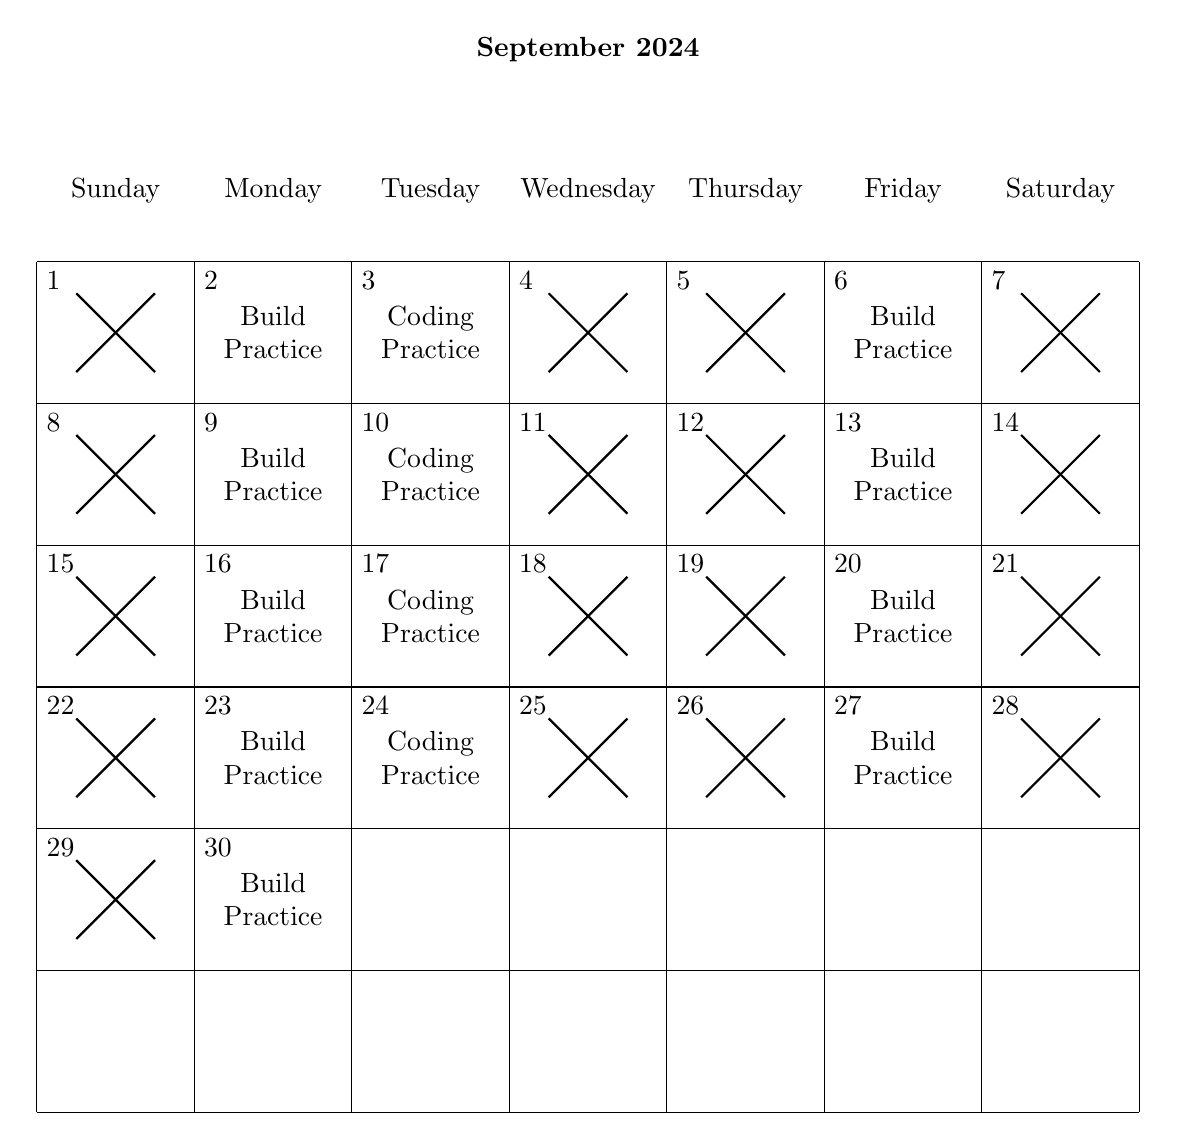
\begin{tikzpicture}
        % Define the dimensions of the calendar
        \def\year{2024}
        \def\month{9}
        \def\monthname{September}
        \def\startday{1} % 1=Sunday, 2=Monday, ..., 7=Saturday
        \def\numdays{30}
        \def\boxwidth{2} % Width of each box
        \def\boxheight{1.8} % Height of each box

\newcommand{\daytext}[1]{
    \ifcase#1
    \or \cross \or Build Practice  \or Coding Practice \or \cross \or \cross \or Build Practice \or \cross \or \cross \or Build Practice \or Coding Practice
    \or \cross \or \cross \or Build Practice \or  \cross \or \cross \or Build Practice \or Coding Practice \or \cross \or \cross \or Build Practice \or  \cross \or \cross \or Build Practice \or Coding Practice \or \cross \or \cross \or Build Practice \or \cross \or \cross \or Build Practice
    \or Coding Practice
    \fi
}

        % Draw the calendar grid
        \foreach \x in {0, 1, 2, 3, 4, 5, 6, 7} {
            \draw (\x*\boxwidth, 0) -- (\x*\boxwidth, -6*\boxheight);
        }
        \foreach \y in {0, -1, -2, -3, -4, -5, -6} {
            \draw (0, \y*\boxheight) -- (7*\boxwidth, \y*\boxheight);
        }

        % Add day labels
        \node at (0.5*\boxwidth, 0.5*\boxheight) {Sunday};
        \node at (1.5*\boxwidth, 0.5*\boxheight) {Monday};
        \node at (2.5*\boxwidth, 0.5*\boxheight) {Tuesday};
        \node at (3.5*\boxwidth, 0.5*\boxheight) {Wednesday};
        \node at (4.5*\boxwidth, 0.5*\boxheight) {Thursday};
        \node at (5.5*\boxwidth, 0.5*\boxheight) {Friday};
        \node at (6.5*\boxwidth, 0.5*\boxheight) {Saturday};

        % Add the dates in the top left corner and specific text in the middle
        \foreach \d in {1,...,\numdays} {
            \pgfmathtruncatemacro{\col}{mod(\d+\startday-2, 7)}
            \pgfmathtruncatemacro{\row}{-(\d+\startday-2)/7}
            \node[anchor=north west] at (\col*\boxwidth, \row*\boxheight) {\d};
            \node[anchor=center, text width=\boxwidth cm, align=center] at (\col*\boxwidth+0.5*\boxwidth, \row*\boxheight-0.5*\boxheight) {\daytext{\d}};
                                        }

        % Add month and year
        \node at (3.5*\boxwidth, 1.5*\boxheight) {\textbf{\monthname\ \year}};
    \end{tikzpicture}
\end{center}
This is what happened during the month of September. We had full team meetings and build practices every Monday and every Friday, and Ian and Jayden had coding practices every Tuesday. Connor had the robot during this time, Ian has been working on the AI, and Jayden has been working on the simulator, which will have a full chapter on it once in place. At the end of the month we have been driving for quite some time and are ready for tournaments in October.
\begin{comment}
\important{Version 2.0 - September 3, 2024}
\chapterauthor{Caleb Bachmeier}
\textbf{Goal}: Breakdown Version 2.0 of V5RC High Stake Game Manual
\section*{Update to Judging}
On September 3rd, 2024 Version 2.0 of the V5RC High Stakes Game Manual was released. This was a major update to the game manual. This chapter will completely cover the update.

\section*{Rule Changes} 
\end{comment}
\important{Team Meeting (September 5, 2024)}
\chapterauthor{Caleb Bachmeier}
\info{Caleb Bachmeier}{Team Meeting}{September 5, 2024}
\section*{Team Meeting}
We have decided to have a team meeting to talk about roles, future tournaments we would be attending, and our future team branding options. 
\section*{Roles}
We wanted to talk about our different team roles and make sure that the entire team was on the same page. For team roles we wanted to have one "main" team member for the role and one-to-two "backups." These are all listed below:
\subsection*{Practice Roles}
\begin{itemize}
    \item Lead Engineer: Connor, Chase, Ian
    \item Lead Coder: Ian, Jayden
    \item Notebook: Caleb, Ian
    \item Driver: Chase, Miles
    \item Social Media: Miles, Chase
\end{itemize}
The first person in the role is the leader of the role, everyone after the role is the backup, someone that understands the role, and can sufficiently do it if that person is gone.
\subsection*{Tournament Roles}
\begin{itemize}
    \item Drive Team: Chase, Miles, Connor
    \item Scout: Connor
    \item Hypeman: Ian
    \item Pit Crew: Jayden, Caleb
\end{itemize}
\section*{Tournaments}
The current list of tournaments we plan to go to include:
\begin{itemize}
    \item Douglas, South Dakota; October 26th
    \item Grand Forks, North Dakota; November 1st - 2nd
    \item Harrisburg, South Dakota; November 23rd
    \item Mitchell, South Dakota; December 7th 
    \item Groton, South Dakota; Early January 
    \item Rapid City, South Dakota; Early February 
    \item Harrisburg, South Dakota (SD State Event); Late February - Early March
    \item Omaha, Nebraska (CREATE US Open); March 27th - March 29th
    \item Dallas, Texas (High School Worlds); May 6th - May 8th
\end{itemize}
The US Open and Worlds are invitation only, so we hope we'll qualify for those. We wanted to have a team meeting because we wanted to find other tournaments to go to. Our current list of possible events include 
\begin{itemize}
    \item Omaha, Nebraska (Robocalypse); September 28th
    \item Omaha, Nebraska (Tom Dickey Memorial); November 2nd
    \item Omaha, Nebraska (Central High School); November 9th 
    \item Omaha, Nebraska (Antler-Wolf-Storm Classic); November 16th
    \item Omaha, Nebraska (Omaha North High School) December 13th - December 14th
\end{itemize}
Broken down tournament by tournament 
\begin{itemize}
    \item Omaha, Nebraska (Robocalypse); September 28th: \\ We don't believe that Chase and Miles would have enough time to practice driving, so this tournament is out of the question 
    \item Omaha, Nebraska (Tom Dickey Memorial); November 2nd: \\ This tournament only has four teams, so we think this one might be canceled 
    \item Omaha, Nebraska (Central High School); November 9th: \\ Like the previous, this tournament has zero teams, and as the date approaches, this tournament will be canceled 
    \item Omaha, Nebraska (Antler-Wolf-Storm Classic); November 16th: \\ Like the previous two this tournament only has one team registered making it likely for it to be canceled 
    \item Omaha, Nebraska (Omaha North High School) December 13th - December 14th: \\ This tournament only has four teams registered, but we know of multiple teams, such as 7686A, that are planning to register, and this tournament over three months to fill-up, and it's only \$100 to enter. This is the tournament for us
\end{itemize}
Looking at all of these tournaments it seems like the only one that is viable for us is Omaha North High School. We will register and start preparing.
\white{October 2024}
\begin{center}
    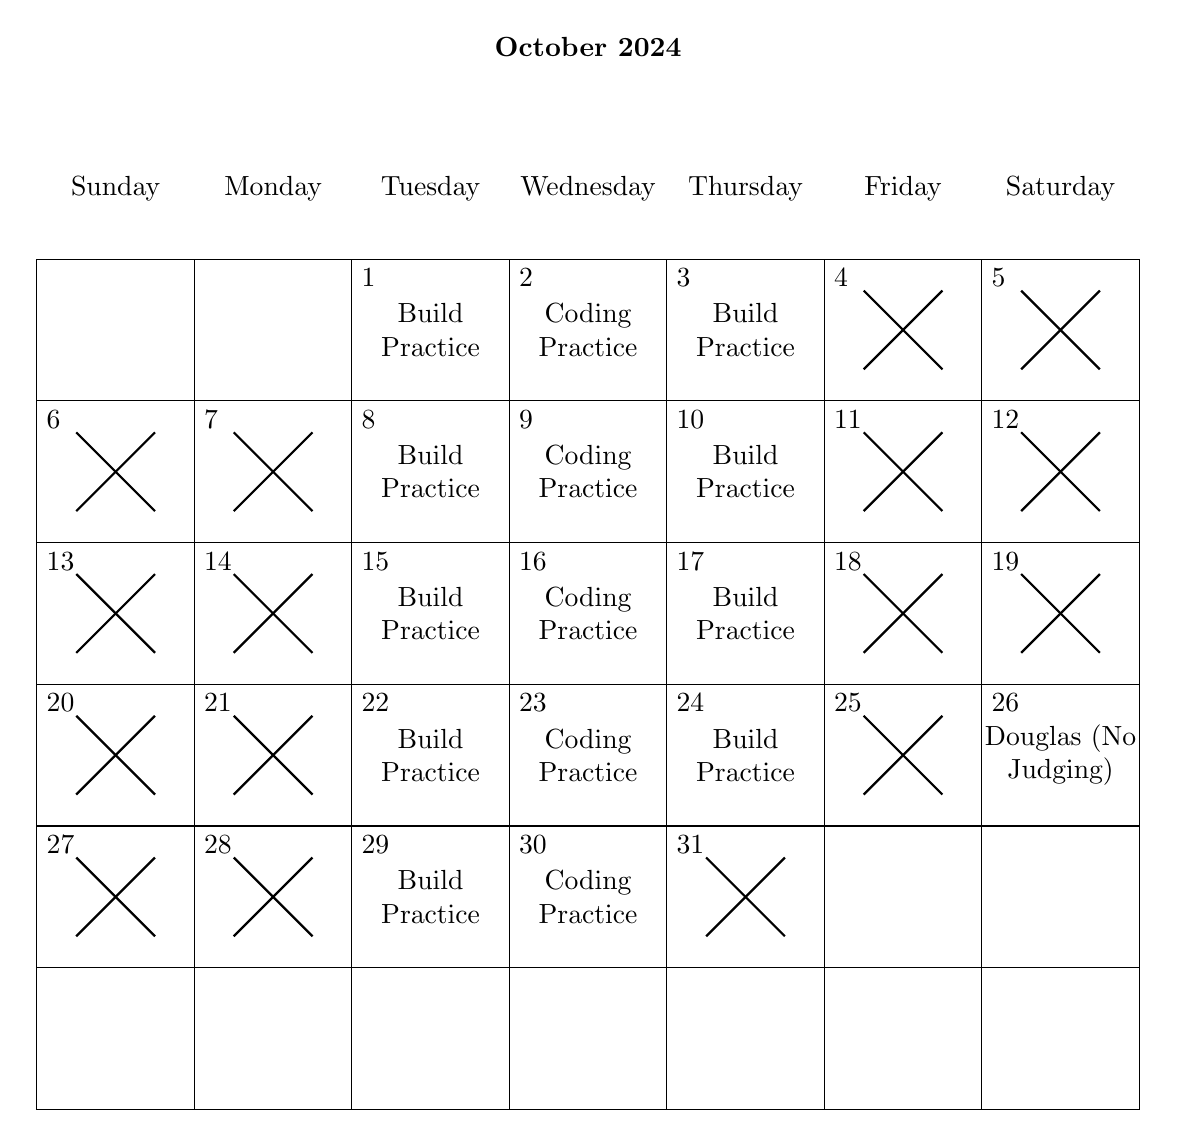
\begin{tikzpicture}
        % Define the dimensions of the calendar
        \def\year{2024}
        \def\month{10}
        \def\monthname{October}
        \def\startday{3} % 1=Sunday, 2=Monday, ..., 7=Saturday
        \def\numdays{31}
        \def\boxwidth{2} % Width of each box
        \def\boxheight{1.8} % Height of each box

\newcommand{\daytext}[1]{
    \ifcase#1
     \or Build Practice  \or Coding Practice \or Build Practice \or \cross \or \cross \or \cross \or \cross \or Build Practice \or Coding Practice
    \or Build Practice \or \cross \or \cross \or \cross \or \cross \or Build Practice \or Coding Practice \or Build Practice \or \cross \or \cross \or  \cross \or \cross \or Build Practice \or Coding Practice \or Build Practice \or \cross \or Douglas (No Judging) \or \cross \or \cross \or Build Practice
    \or Coding Practice \or \cross
    \fi
}

        % Draw the calendar grid
        \foreach \x in {0, 1, 2, 3, 4, 5, 6, 7} {
            \draw (\x*\boxwidth, 0) -- (\x*\boxwidth, -6*\boxheight);
        }
        \foreach \y in {0, -1, -2, -3, -4, -5, -6} {
            \draw (0, \y*\boxheight) -- (7*\boxwidth, \y*\boxheight);
        }

        % Add day labels
        \node at (0.5*\boxwidth, 0.5*\boxheight) {Sunday};
        \node at (1.5*\boxwidth, 0.5*\boxheight) {Monday};
        \node at (2.5*\boxwidth, 0.5*\boxheight) {Tuesday};
        \node at (3.5*\boxwidth, 0.5*\boxheight) {Wednesday};
        \node at (4.5*\boxwidth, 0.5*\boxheight) {Thursday};
        \node at (5.5*\boxwidth, 0.5*\boxheight) {Friday};
        \node at (6.5*\boxwidth, 0.5*\boxheight) {Saturday};

        % Add the dates in the top left corner and specific text in the middle
        \foreach \d in {1,...,\numdays} {
            \pgfmathtruncatemacro{\col}{mod(\d+\startday-2, 7)}
            \pgfmathtruncatemacro{\row}{-(\d+\startday-2)/7}
            \node[anchor=north west] at (\col*\boxwidth, \row*\boxheight) {\d};
            \node[anchor=center, text width=\boxwidth cm, align=center] at (\col*\boxwidth+0.5*\boxwidth, \row*\boxheight-0.5*\boxheight) {\daytext{\d}};
                                        }

        % Add month and year
        \node at (3.5*\boxwidth, 1.5*\boxheight) {\textbf{\monthname\ \year}};
    \end{tikzpicture}
\end{center}
This is what happened during the month of October. We had full team meetings and build practices every Tuesday and every Thursday, and Ian and Jayden had coding practices every Tuesday. Ian and Jayden are very close in their respective coding endeavors and will be documenting and implementing in our two planned tournaments on October 26, in Douglas, South Dakota; and on November 1 and 2 in Grand Forks, North Dakota.
\begin{comment}
\important{Autonomaus Planning}
\chapterauthor{Caleb Bachmeier}
\info{Caleb Bachmeier}{}{}
\end{comment} %September 6
\identify{Identify the Challenge \& Set Goals: Arm V1.1 (September 28th, 2024)}
\info{Connor Albers}{Arm}{September 28th, 2024}
\chapterauthor{Connor Albers}
\label{chap:ArmV1.1}
\textbf{Goal}: We will identify an objective for our robot so that we can address it and build an effective solution
\section*{Problem Statement}
Our challenge was to create an effective arm mechanism for picking up rings while adhering to size constraints and ensuring functionality with existing components.

\section*{Solution Requirements}
\begin{itemize}
    \item The arm must be able to pick up rings reliably.
    \item It should fit within the robot's starting size.
    \item The mechanism must minimize motor usage due to limited availability.
\end{itemize}

\section*{Solution Goals}
\begin{itemize}
    \item Achieve a minimum of 80\% efficiency in ring pickup.
    \item Maintain a simple and effective design.
\end{itemize}


\brainstorm{Brainstorm \& Diagram: Arm V1.1 (September 28th, 2024)}
\info{Connor Albers}{Arm}{September 28th, 2024}
\chapterauthor{Connor Albers}
\section*{Possible Solution - Victory Arm}
One design in particular that caught our attention was 1168A, Victory’s arm. As shown in our bibliography: "\cite{1168APitsandParts}"
Their design used the same arm design as the redirect we had already constructed but swapped the basket and accompanying pneumatic with a simple claw.
\begin{figure}[H]
    \centering
    \includegraphics[width=0.5\linewidth]{images/Victory Arm Pits and Parts Thumbnail.png}
    \caption{\cite{1168APitsandParts}}
    \label{fig:1168A}
\end{figure}

\noindent
\textbf{Pros}:
\begin{itemize}
    \item Utilizes pneumatics, freeing up motors for other mechanisms.
    \item Greater leverage and range of motion.
\end{itemize}
\textbf{Cons}:
\begin{itemize}
    \item Potentially complex pneumatic setup.
    \item Requires careful positioning to avoid interference with the intake mechanism.
\end{itemize}

\section*{Possible Solution - Net Mechanism}
A "Net" Mechanism would take the Ring off of our Intake, using something similar to a catapult 

\begin{figure}[H]
    \centering
    \includegraphics[width=0.5\linewidth]{images/Fishmech.jpg}
    \caption{Net Mechanism}
    \label{fig:fish-mech}
\end{figure}

\noindent
\textbf{Pros}:
\begin{itemize}
    \item Utilizes pneumatics.
    \item Greater leverage and range of motion.
    \item Very simple build
\end{itemize}
\textbf{Cons}:
\begin{itemize}
    \item Requires careful positioning to avoid interference with the intake mechanism.
\end{itemize}

\solution{Choose a Solution: Arm V1.1 (September 29, 2024)}
\info{Connor Albers}{Arm}{September 29th, 2024}
\chapterauthor{Connor Albers}
\section*{Choose a Solution}
\renewcommand{\arraystretch}{1.85} % Change this value as needed
\begin{table}[htb!]
\centering
\begin{tabular}{|>{\centering\arraybackslash}m{1.85cm}|>{\centering\arraybackslash}m{1.85cm}|>{\centering\arraybackslash}m{1.85cm}|>{\centering\arraybackslash}m{1.85cm}|>{\centering\arraybackslash}m{1.85cm}|>{\centering\arraybackslash}m{1.85cm}|>{\centering\arraybackslash}m{1.85cm}|}
\hline
\textbf{Scale 1 - 10} & \textbf{Simplicity} & \textbf{Reliability} & \textbf{Traction} & \textbf{Size} & \textbf{Speed} & \textbf{Total} \tabularnewline
\hline
Weight & x1 & x3 & x2 & x1 & x3 & \tabularnewline
\hline
Net Mechanism & 5 & 10 & 6 & 10 & 6 & 75 \tabularnewline
\hline
Victory Arm & 3 & 10 & 10 & 10 & 6 & 81 \tabularnewline
\hline
\end{tabular}
\caption{Arm Decision Matrix}
\label{tab:drive-matrix}
\end{table}
\renewcommand{\arraystretch}{1.85} % Reset to default
According to our point totals it seems that we will use 1168A, Victory's Arm. Lets make a plan in CAD. 
\section*{Make a Plan}
\begin{figure}[H]
    \centering
    \includegraphics[width=1\linewidth]{images/Arm Drawing.jpg}
    \caption{Fusion 360 Arm Drawing}
    \label{fig:arm-drawing}
\end{figure}
\build{Build \& Program: Arm V1.1 (September 29th, 2024)}
\info{Connor Albers}{Arm}{September 29th, 2024}
\chapterauthor{Connor Albers}
\section*{Building}
\section*{Disassembly}
To start, we took off our basket and the pneumatic attached to it. 

\section*{Arm Modification}
Next, we swapped out the two main C-channels on the arm for full-length 35-hole ones.

\section*{Engineering the Claw}
The next step was to engineer the claw. Much like our previous design, the claw pivoted at the end of our arm but, unlike our previous design, it used rubber bands to force it out. 

The reason the claw needed to pivot was because it was at the front of our robot, meaning it would be hit every time we ran into something, which happens often during competition. Allowing the claw to pivot meant that every time we hit something, the claw would be pushed into the high-strength axle across our intake, and all the force would be transferred into it rather than into the arm itself.

\section*{Using L-Channels}
We used L-channels as the pieces that pivoted on the end of the arm (see Figure~\ref{fig:ichannelsendofarm}) because of their lightweight construction. Making our arm as light as possible was crucial to ensuring our arm would still work at lower air pressures. 

\begin{figure}[H]
    \centering
    \includegraphics[width=0.7\textwidth]{images/Ichannelsendofarm.png}
    \caption{L-channels at the end of the arm.}
    \label{fig:ichannelsendofarm}
\end{figure}

By attaching pillow bearings to the L-channels (see Figure~\ref{fig:pillowbearings}), we were able to provide a spot for each side of our claw to pivot on. 

\begin{figure}[H]
    \centering
    \includegraphics[width=0.7\textwidth]{images/Pillowbearings.png}
    \caption{Pillow bearings attached to L-channels.}
    \label{fig:pillowbearings}
\end{figure}

\section*{Claw Construction}
Each “finger” of the claw was constructed using a 1x2 C-channel and an L-channel to provide mounting for our pneumatic (see Figure~\ref{fig:clawfinger}). 

\begin{figure}[H]
    \centering
     \includegraphics[width=0.7\textwidth]{images/clawfinger.png}
    \caption{Claw finger constructed with C-channel and L-channel.}
    \label{fig:clawfinger}
\end{figure}

\section*{Adding the Pneumatic}
The last step to complete our claw was to add the pneumatic. For this, we used a 50mm dual-action piston. After adding tubing and wiring to the pneumatic, our claw and arm assembly were completed.
%Add subsections about different building parts 
\test{Test the Solution: Arm V1.1 (September 30th, 2024)}
\section*{Test the Solution} %September 30
\white{Fusion 360}
\chapterauthor{Connor Albers}
\section*{The Importance of Designing Before Building}  
\info{Connor Albers}{Fusion 360}{October 4, 2024}
Designing your robot before actually building it is important for any team, as it allows potential problems to be solved prior to construction, preventing wasted parts. It also enables teams to explore different ideas faster and more efficiently. For many teams, a simple drawing is all they need to get started building, but our team decided to go the digital route with computer-aided design (CAD). Using CAD allows our team to not only view our designs in 3D but also aids us in designing to scale, ensuring every piece fits just as it would in real life.

\section*{Options for CAD Software in VEX Robotics}  
When designing VEX robots specifically, there are many options, such as Onshape or Fusion 360. Both programs are popular within the VEX community and thus have large file folders containing 3D models of every official VEX part. These folders make it easy to import parts and design robots more efficiently, removing the need to download parts individually from the VEX website.

\section*{Advantages and Challenges of Using CAD}  
While these software platforms feature steep learning curves for new users, they offer many benefits. Importing parts manually means users can add new parts just as they are released on the VEX official website. Additionally, teams may import or create custom parts to fit their specific needs. These custom parts can then be laser-cut, CNC-machined, or 3D-printed to create components accurately.

\section*{Collaboration and File Exporting}  
Collaboration is another key advantage of these software platforms; both allow the user to add others to documents, promoting teamwork within the group. Additionally, these more generic CAD programs allow the user to export files in industry-standard formats, enabling the team to accurately simulate their robot in other programs.

\section*{Protobot: A User-Friendly Alternative}  
Another, more user-friendly option is a community project called Protobot. Protobot is software that allows users to create robots virtually using VEX parts. What’s special about this software is that it is designed specifically for VEX V5 robot construction, so every part is imported and ready to use. Combined with optimized part-collaging features, Protobot is the most user-friendly CAD program for designing VEX robots.

\section*{Drawbacks of Protobot}  
This accessibility does have its drawbacks. First, the parts catalog is not always up to date; new parts may take an extended period to be added to the program. Second, as of October 2024, the software does not support live file sharing, meaning the only way to share models is to download and send them via email or other mediums, making collaboration difficult. Finally, the software does not allow users to import or design custom parts, making it challenging for advanced teams to accurately construct their robots.

\section*{Why We Chose Fusion 360}  
With all this information in mind, our team decided to use Fusion 360 to design our future robots. Fusion 360 was the obvious choice for our team because many of our members already had experience using the program. Also, from what we had heard from other teams, Fusion was far more powerful than other programs, such as Onshape, due to it running locally on the user’s device rather than over the cloud. A final advantage of using a generic CAD program is that we planned on creating a virtual simulation, which would require standard files not supported in Protobot.

\important{Pre Douglas Coding (October 10, 2024)}
\chapterauthor{Ian Smith}
\info{Ian Smith}{Pre Douglas Coding}{October 10, 2024}
\section*{Coding in Robot Design}

Coding is a very critical part of robot design, especially when considering the most current mechanical design. Within the software, we will have to perform complex kinematics, graphic design, and dynamic programming within the C++ language. The coding of this bot started with an accurate LemLib setup for our bot.

%\begin{lstlisting}[language=C++, caption={LemLib Setup}, label={lst:lemlib_setup}]
%(insert code here)
%\end{lstlisting}

I wrote the basic controls for the pneumatics on a toggle and implemented expo drive. After a meeting with the drive team, a few concepts were discussed:
\begin{itemize}
    \item Displaying match status on the brain
    \item Displaying match status on the controller
    \item Custom controller layouts for both drivers
    \item Motor status during a match (color-coded on the brain)
    \item Chase proposed the idea of using both controllers (buddy controller), but switchable
\end{itemize}

Knowing that all the requested ideas were feasible within the hardware, I knew I could write a software solution to meet the design requirements. 

\subsection*{Switchable Controllers}
I first decided to tackle the switchable controllers as this seemed to be the most relevant feature. I created a class called \texttt{my\_controller} that contained public variables for each button and mapped control. Originally, I used the \texttt{int} variable type because the enumerated values within the \texttt{pros} namespace expand into small integers. However, this didn’t work, and I had to switch to the \texttt{pros::controller::E\_DIGITAL\_PRESSING} type. This correctly allowed button mapping on the controllers, varied by different instances of the class.

I declared the subsequent class and initialized the mapping for each user. Another instance, called \texttt{current}, had the currently selected controller class instance written to it. A function was created to determine which controller was current based on the last “give away” or “switch controller” button. 

There were a few issues overall, primarily due to the \texttt{get\_digital} functions only accepting special \texttt{pros} variable types for buttons, along with issues in passing controller objects by reference. However, overall, the implementation was quick and easy.

\subsection*{Motor Status Color Coding}
The next challenge I undertook was adding color coding for motor states based on temperature. I knew that motors cut out in increments, but I didn’t know the specifics. The general idea was that the motors would reduce their maximum power, and we could display this on the brain. 

For this, I referred to a VEX Forum post (\href{https://www.vexforum.com/t/v5-motor-temp-in-percent/52433}{https://www.vexforum.com/t/v5-motor-temp-in-percent/52433}) and used the response by \texttt{jpearman}. I set up circles on the V5 brain to coordinate with the eight motors on the robot, filling them with the appropriate color (green, yellow, or red) depending on motor state. Initially, I encountered arithmetic and color errors when trying to print to the brain.

\subsection*{Future Features}
The drivers are requesting a “Print to Controller” system for mid-match monitoring. I haven't implemented this yet due to time constraints. I also sketched out a few mock autonomous routines for LemLib, though I am still experiencing issues with my IMU and rotational PID. The autonomous routines are selected on an autonomous selection screen, which consists of boxes activated by a \texttt{when\_pressing()} function.

\section*{LemLib: An Overview and Implementation}  

LemLib is a student-developed, open-source library for VEX VRC that is feature-rich and easy to use \href{https://github.com/LemLib/LemLib}{(this is a link to the LemLib GitHub project)}. After successfully writing my own PID controller and beginning work on a pure pursuit algorithm, I realized that using a library would streamline the development of our autonomous routines—something I could have implemented from scratch but found more efficient through LemLib.  

In order to use LemLib, the process revolves around a few simple principles.  

\subsection*{Setting up LemLib}  
The first step was importing the LemLib depot from GitHub into my development environment.  
\begin{quote}
\textbf{Author's Note:} I am using Ubuntu 22.04 with the PROS extension over Visual Studio Code as my setup.  
\end{quote}

The LemLib documentation provides clear examples on how to import the library. In the PROS terminal, I executed the following commands:  

\begin{verbatim}
$ pros c add-depot LemLib https://raw.githubusercontent.com/LemLib/LemLib/depot/stable.json
$ pros c apply LemLib
\end{verbatim}

\subsection*{Initializing Motors and Sensors}  
After importing the library, the next step was to add the appropriate motors and motor groups. Since we are using an Inertial Measurement Unit (IMU) to measure the robot’s heading ($\theta$), we had to declare an instance of the IMU class. Initially, we encountered an issue with the IMU, as the heading value continuously decreased when the robot was stationary. To resolve this, we replaced the faulty IMU with the one from Capten’s Worlds robot.  

The next task was to initialize the sensors for odometry. Although we originally planned to use an odometry pod, we did not have enough space on our robot. As a substitute, we used the drivetrain's motor encoders (IMEs), which are less accurate but still functional for tracking. Afterward, I created an instance of the \verb|sensors| class, passing in the necessary configuration parameters.  

We also utilize the controller curves provided by LemLib, as discussed in Chapter . All this information is combined to create an instance of the \verb|drivetrain| class.  

\subsection*{Initializing the Chassis}  
Within the initialization loop, we had to declare:  

\begin{verbatim}
chassis.initialize();
\end{verbatim}

At this point, our code was ready to be tuned.  

\paragraph{Note:}  
For months, we faced issues with the chassis not initializing properly. After countless hours of troubleshooting and communicating with the developers, we finally identified the problem. Our code mistakenly included:  

\begin{verbatim}
void initalize() {}
\end{verbatim}

The correct code should have been:  

\begin{verbatim}
void initialize() {}
\end{verbatim}

Did you spot the difference? That missing letter in the function name caused all our issues!  

\subsection*{Tuning the Autonomous Functions}  
When tuning the autonomous routines, we began with the angular PID (Proportional-Integral-Derivative) controller. We started with a small proportional gain ($k_P$) and gradually increased the derivative gain ($k_D$) until the robot stopped with high accuracy while maintaining maximum speed into a stop.  

In this scenario, tuning the integral gain ($k_I$) was unnecessary since the robot did not need to maintain specific positions—such as holding an arm steady. The same procedure was followed for the lateral PID controller, ensuring the robot was fully tuned.  

\subsection*{Implementing Pure Pursuit Paths}  
With our PID tuning complete, the next step is to input the paths from our concepts into LemLib’s pure pursuit algorithm. We plan to complete this task in the days leading up to the Douglas competition.  

\subsection*{Conclusion}  
Our LemLib implementation is now fully documented and explained, providing a solid foundation for our robot’s autonomous capabilities. The skeleton project ensures that all aspects are correctly configured and ready for testing.



\white{Robot V1 (October 16, 2024)}
\chapterauthor{Caleb Bachmeier}
\info{Caleb Bachmeier}{Robot V1}{October 16, 2024}
\textbf{Goal}: This chapter will explain our first robot
\section*{Robot V1}
Below are complete pictures of our first robot in Fusion 360:
%Pictures of the robot in fusion 360
\subsection*{Drivetrain}
Drivetrain stats:
\begin{itemize}
    \item 66 Watts
    \item 480 RPM
    \item 14.75"
    \item Peak velocity is 82/inches per second
\end{itemize}
\begin{figure}[hbt!] % Use [hbt!] to place the figures on the same page
    \begin{minipage}{.5\textwidth}
        \centering
        \includegraphics[width=.8\linewidth]{images/Frontdown-V1-Drivetrain.png}
        \caption{Front view}
        \label{fig:frontdown}
    \end{minipage}
    \begin{minipage}{.5\textwidth}
        \centering
        \includegraphics[width=.8\linewidth]{images/Iso-V1-Drivetrain.png}
        \caption{Isometric view}
        \label{fig:iso}
    \end{minipage}
    \begin{minipage}{.5\textwidth}
        \centering
        \includegraphics[width=.8\linewidth]{images/Topdown-V1-Drivetrain.png}
        \caption{Top view}
        \label{fig:topdown}
    \end{minipage}
    \begin{minipage}{.5\textwidth}
        \centering
        \includegraphics[width=.8\linewidth]{images/Sidedown-V1-Drivetrain.png}
        \caption{Side view}
        \label{fig:sidedown}
    \end{minipage}
\end{figure}

Above are our finished drivetrain CAD images.
\subsection*{Clamp}
Clamp stats:
\begin{itemize}
    \item Uses two, 12 pound, pneumatic pistons 
    \item Clamps the corner of 
\end{itemize}
\begin{figure}[h!] % Use [hbt!] to place the figures on the same page
    \begin{minipage}{.55\textwidth}
        \centering
        \includegraphics[width=1\linewidth]{images/Iso-Clamp-V1.png}
        \caption{Isometric View}
        \label{fig:iso}
    \end{minipage}
    \begin{minipage}{.55\textwidth}
        \centering
        \includegraphics[width=1\linewidth]{images/Front-Clamp-V1.png}
        \caption{Front View}
        \label{fig:front}
    \end{minipage}
    \begin{minipage}{.55\textwidth}
        \centering
        \includegraphics[width=1\linewidth]{images/Side-Clamp-V1.png}
        \caption{Side View}
        \label{fig:side}
    \end{minipage}
    \begin{minipage}{.55\textwidth}
        \centering
        \includegraphics[width=1\linewidth]{images/Bottom-Clamp-V1.png}
        \caption{Bottom View}
        \label{fig:bottom}
    \end{minipage}
\end{figure}

Above are pictures of our Clamp in Fusion 360
\subsection*{Hook Intake}
Hook Intake stats:
\begin{itemize}
    \item Uses 22 watts of power
    \item Uses acetal hooks to grab rings and place them on Mobile Goals
\end{itemize}

\subsection*{Robot V1}
This is our entire first robot or Robot V1. Below are Fusion 360 pictures of the entire thing, the only thing it is missing is the chain on the Hook Intake.
 %October 16
\important{Simulation}
\chapterauthor{Jayden Yanzick}
\info{Jayden Yanzick}{Simulation}{October 18, 2024}
\label{simulation}

\section*{Intro to the AI}
As AI grows into our everyday lives, so too does it grow into the field of robotics. Every year, more companies around the world digitalize into new AI models to manage their algorithms and systems more efficiently. Because of that, I would like to present my side of AI, with an AI simulator that's been in development since May of this year. Using complex algorithms and various mathematical concepts, its purpose is to create the best skills run designed for our bot and the field.

\section*{The Simulator as a Whole}
The simulator used is called Webots. It is a digital robotics simulator that allows for unlimited design possibilities, using different programming languages to control bots. In this case, I am designing a simulator containing the field, the bot, and a neural network utilizing Deep Reinforcement Learning. Webots uses \textit{Nodes} to define objects in the simulated world, which enables the bot to interact with the environment. There are many types of nodes, but I will focus only on the main ones used in our project.

\begin{figure}
    \includegraphics[width=0.9\linewidth]{images/simsoftware}
    \captionof{figure}{The Simulation Software} % Use \captionof instead of \caption
    \label{fig:simsoftware}
\end{figure}

\section*{CAD Designing and Modeling}
To design the bot inside the simulator, we use Fusion 360 to create CAD models. While Webots does offer basic shape modeling (e.g., cubes, spheres, cones), more complex parts require external CAD software. These models allow us to visualize designs in a digital environment without risking damage to the physical bot. The CAD models are optimized for memory efficiency and integrated into the simulator using Nodes. Game objects and field elements are imported directly from the CAD files provided by VEX.

\section*{Deep Reinforcement Learning and the Neural Network}
Our neural network is based on Deep Reinforcement Learning (DRL). DRL combines two concepts:  
- \textbf{Deep Learning:} Enables the network to make decisions based on the state of the field, such as the location of game objects and the bot’s position.  
- \textbf{Reinforcement Learning:} Involves multiple "episodes," where each episode is a complete skills run. The neural network learns through these repeated episodes, improving its performance by recognizing scoring opportunities and efficient strategies.

\begin{figure}
    \includegraphics[width=0.9\linewidth]{images/neuralexample}
    \captionof{figure}{An example of a neural network.}
    \label{Fig:neuralexample}
\end{figure}

In the current configuration, the network consists of 4 input neurons, 512 hidden neurons, and 1 output neuron. The output determines the bot's actions. Here’s a simplified example of how the code processes the output:

\begin{verbatim}
double action = 1.0;
round(1, action * 2);
if (action == 1) {
    // movement function
}
\end{verbatim}

This code multiplies the output by 2 and rounds it to a whole number. The result triggers a specific function, which executes the desired action. The process repeats, allowing the network to learn through trial and error.

\section*{Programming the Main Bot}
The main robot is controlled through a \textit{Supervisor} node, which grants it additional capabilities. This allows the bot to manage the simulation independently. The robot’s components include:
\begin{itemize}
    \item Seven motors: Six for the drivetrain, one for a hook to grab goals.
    \item Receiver and Emitter nodes: Used for communication with other bots.
\end{itemize}

To initialize devices within Webots, you must define them in code, as shown below:

\begin{verbatim}
#include <webots/Robot.hpp>
#include <webots/Motor.hpp>

using namespace webots;

Robot *robot = new Robot();
Motor *example = robot->getMotor("example");
\end{verbatim}

The \verb|#include| statements import the required classes, enabling the creation of the robot and its components. The code is organized across multiple files, with the primary file named after the controller (e.g., \verb|<controller_name>.exe|). Devices are defined separately, while functions are organized within classes.

\begin{figure}[h]
    \centering
    \caption{The first 27 lines of initializing devices in the simulator.}
    \includegraphics[width=0.9\linewidth]{images/initalizing.png}
\end{figure}

We use four classes to organize the code:
\begin{itemize}
    \item \textbf{Bot:} Contains functions for the robot.
    \item \textbf{Sim:} Manages simulation-related functions.
    \item \textbf{NeuralNetwork:} Handles the neural network’s operations.
    \item \textbf{Reset:} Manages manual resets of the simulation.
\end{itemize}

\section*{Programming the Scoring Bot}
The scoring bot operates with a separate controller, as each robot requires its own controller. It uses \textit{Camera} and \textit{Connector} nodes to track goals and count rings. The camera can detect predefined object colors, allowing the bot to calculate the score accurately. Here’s a sample of the scoring logic:

\begin{verbatim}
switch (objectCount) {
    case 1:
        currentScore += 3;
        break;
    case 2:
        currentScore += 4;
        break;
    // intervals increase by 1 for each additional ring
}
\end{verbatim}

The score is printed to the console and sent to the neural network through an Emitter node, allowing the network to adjust weights based on the run’s outcome.

\begin{figure}[h]
    \includegraphics[width=0.9\linewidth]{images/simfield.png}
    \centering
    \caption{The field with camera overlays.}
    \label{Fig:simfield}
\end{figure}

\section*{Training the Neural Network}
Before the training begins, the two bots perform a radio check to confirm communication. The neural network then initiates random actions within the field. Once the simulation timer expires, the final score is pushed to the network, which updates the weights of the neurons. The simulator resets, and the training loop starts again for the next run.
 %October 18
\white{Douglas Tournament Overview: (October 26, 2024)}
\chapterauthor{Caleb Bachmeier}
\info{October 26, 2024}{Douglas Tournament Overview}{Caleb Bachmeier}
\textbf{Goal:} Analyze the tournament in Douglas, South Dakota
\section*{General Tournament Information}
\begin{itemize}
    \item \textbf{Tournament Name:} DOUGLAS PATRIOTS High Stakes
    \item \textbf{Date:} 26th of October, 2024
    \item \textbf{Location:} Douglas, South Dakota
    \item \textbf{Winning Teams:} 7686A  - 6844B
\end{itemize}

\section*{Performance Information}
\begin{itemize}
    \item \textbf{Record for Qualification Matches}: 4/4/0 50\% win percentage
    \item \textbf{Alliance Selection:} 82728B
    \item \textbf{Finals:} We lost in semifinals
\end{itemize}
\subsection*{Qualification: 4}

\begin{itemize}
    \item \textbf{Blue Alliance:} 82718E - 7686H
    \item \textbf{Red Alliance:} 89910A - 7686X
    \item \textbf{Score:} \colorbox{cyan}{27} \colorbox{red}{11}
    \item \textbf{Autonomous Winner: Blue}
    \item \textbf{Our Strategy}: We planned to have Chase and Miles to fill up as many Mobile Goals as they can. During this, we would have our teammates, 89910A, sit in the Positive Corner until we gave them a filled Mobile Goal to put into the corner. 
    \item \textbf{How the match went}: When the Autonomous Period started, our robot just started spinning around and didn't score any points. When we started Driver Control teammates went into the Positive Corner, like they should've, but once they were in there, their robot had a fatal error and couldn't move. Also once we had three Rings on a Mobile Goal, a Ring fell off our Intake, and into the inner workings of the robot, this prevented us from scoring any more Rings on a Mobile Goal.
    \item \textbf{What We Can Learn:} Having a good backup plan will be very useful in the future. We aren't sure on what happened with our Autonomous program, but we can figure that out.
\end{itemize}

\subsection*{Qualification: 10}

\begin{itemize}
    \item \textbf{Blue Alliance:} 7686X - 7686N
    \item \textbf{Red Alliance:} 9050E - 99515A
    \item \textbf{Score: \colorbox{cyan}{12}
    \colorbox{red}{2}}
    \item \textbf{Autonomous Winner:} Tie
    \item \textbf{How the match went}: Autonomous: Nobody's robot did anything during autonomous.. Driver: we quickly put two three Ring, Mobile Goals into the Positive corners, this remained consistent until 9050E clamped onto our Positive corner within the protected period, disqualifying them. Then we went over and grabbed the Mobile Goal and put it in the Positive corner - illegally. This disqualified us technically losing us the match.
\end{itemize}

\subsection*{Qualification: 13}

\begin{itemize}
    \item \textbf{Blue Alliance:} 9050B - 7686X
    \item \textbf{Red Alliance:} 89910A - 82718G
    \item \textbf{Score: \colorbox{cyan}{20} \colorbox{red}{0}}
    \item \textbf{Autonomous Winner:} Blue
    \item \textbf{Our Strategy}: Our strategy was the same as Qualification 4, have our teammates camp the positive corners, until we filled up a Mobile Goal to put in it.
    \item \textbf{How the match went}: We started off by scoring one Blue Ring on a Mobile Goal in the Autonomous period. Not as well as we'd like, but no other team on the field had a Autonomous program, so the Autonomous win was guaranteed. After Driver Control period started we filled up a Mobile Goal with five Blue Rings. We would like to get six rings, but we had an opportunity to place it in the Positive Corner, so we took it. But when we were placing it we high centered ourselves on a Ring, unfortunately this means we couldn't move anymore. Because of this we had our teammates help us guard the Mobile Goal in the corner. This worked very well because, although they tried, the Red Alliance couldn't score at all.
    \item \textbf{What We Can Learn}: 
\end{itemize}

\subsection*{Qualification: 27}

\begin{itemize}
    \item \textbf{Blue Alliance:} 6844B - 7686X
    \item \textbf{Red Alliance:} 6844E - 57437A
    \item \textbf{Score: \colorbox{cyan}{39} \colorbox{red}{3}}
    \item \textbf{Autonomous Winner:} Blue
    \item \textbf{How the match went}:We got two full Mobile Goals in the Positive corner after a successful Autonomous program. We had great coordination, 6844B might be a good Alliance partner
\end{itemize}

\subsection*{Qualification: 34}

\begin{itemize}
    \item \textbf{Blue Alliance:} 7686A - 7686X
    \item \textbf{Red Alliance:} 82718A - 99515B
    \item \textbf{Score: \colorbox{cyan}{29} \colorbox{red}{3}}
    \item \textbf{Autonomous Winner:} Blue
    \item \textbf{Our Strategy}: Autonomous was great both of ours worked and we got AWP. In driver we disconnected halfway through the match, we need to look into this

\end{itemize}

\subsection*{Qualification: 42}

\begin{itemize}
    \item \textbf{Blue Alliance:} 7686H - 99515C
    \item \textbf{Red Alliance:} 7686X - 57783B
    \item \textbf{Score: \colorbox{cyan}{8} \colorbox{red}{6}}
    \item \textbf{Autonomous Winner:} Tie
    \item \textbf{How the match went}: Autonomous: Our program didn't do anything, but nobody's else did anything either. Our Robot lost connection halfway through the match, leading to a grueling loss. 
\end{itemize}

\subsection*{Quarterfinals}
\begin{itemize}
    \item \textbf{Blue Alliance:} 7686N - 82718A
    \item \textbf{Red Alliance:} 82718B - 7686X
    \item \textbf{Score: \colorbox{cyan}{0} \colorbox{red}{22}}
    \item \textbf{Autonomous Winner:} Red
    \item \textbf{How the match went}:  We got two almost full Mobile Goals in each Positive corner. In the final seconds, we took Red's Mobile Goals and put them in the Negative Corner.
\end{itemize}
\subsection*{Semifinals}
\begin{itemize}
    \item \textbf{Blue Alliance:} 82718B - 7686X
    \item \textbf{Red Alliance:} 7686A - 6844B
    \item \textbf{Score: \colorbox{cyan}{2} \colorbox{red}{26}}
    \item \textbf{Autonomous Winner:} Red
    \item \textbf{How the match went}: Autonomous: everyone had a program that worked, we just lost. In driver the Red Alliance got both of their Mobile Goals in the Positive Corners. In the final protected period, 7686A took our two Mobile Goals and put them in the Negative Corners
\end{itemize}

\section*{Coding}
\subsection*{Pre-Tournament Preparation}
All code was working going into the tournament, minus a slight electrical issue with one of our drive motors that we noticed during our pre-tournament scrimmages. We started the day using two controllers, still keeping the switchable function enabled.

\subsection*{Early Matches and Initial Problem}
After two matches, both drivers decided that they no longer wanted the switchable feature. They encountered issues selecting the correct program before matches—mainly due to a buggy autonomous (auton) selector when switching between control loops.

In a rush to fix the code before the next match, I quickly applied what seemed to be the fastest solution. Without fully considering the long-term impact, I commented out the assignment of:
\begin{minted}[linenos, fontsize=\small]{cpp}
switch_button = pros::Controller::E_DIGITAL_B;
\end{minted}
\subsection*{Unexpected Issue with the Controller}
While this seemed to work momentarily, I overlooked an important detail: the default constructor for \texttt{switch\_button} within the \texttt{my\_controller} class was:
\begin{minted}[linenos, fontsize=\small]{cpp}
pros::Controller::E_DIGITAL_DOWN;
\end{minted}

During the next match, the robot stopped functioning entirely. Initially, we blamed field control for the issue. However, when the problem recurred across multiple matches, I suspected it was a programming issue—but I couldn’t recall making significant changes that would have caused it.

\subsection*{Finding the Bug and Implementing the Fix}
After some investigation and reviewing the code, I realized the problem: when the driver tried to use the mobile goal clamp, the controller was automatically switching from \texttt{master} to \texttt{slave}. However, the \texttt{slave} controller was not connected to field control or even present near the field.

The solution involved reinstating the switch button in the code and disabling the switching functionality entirely. This quick fix worked just in time for our next match.

\subsection*{Outcome and Lessons Learned}
Unfortunately, due to the bug, we lost three matches—largely due to an easy strength of schedule that could have been managed better without the issue. While the temporary fix solved the immediate problem, the experience highlighted the importance of thorough testing, even under time constraints.

\section*{Strategy Analysis}
\begin{itemize}
    \item \textbf{Overall Tournament Strategy:} [Summary of the General Tournament Strategy]
    \item \textbf{Strengths:} [Strengths of the Team and Robot]
    \item \textbf{Weaknesses:} [Weaknesses or Areas for Improvement]
    \item \textbf{Adaptability:} [How the Team Adapted to Opponents]
    \item \textbf{Key Matches:} [Analysis of Key Matches]
\end{itemize}

\section*{Lessons Learned}
\begin{itemize}
    \item \textbf{Technical Improvements:} [Ideas for Technical Improvements]
    \item \textbf{Strategic Adjustments:} [Adjustments to Strategy]
    \item \textbf{Preparation Tips:} [Tips for Future Preparation]
    \item \textbf{Overall Record For Douglas}: 4/4/0 50\%
    \item \textbf{Overall Record for High Stake}: 4/4/0 50\%
\end{itemize}
Our next tournament is in less than a week in Grand Forks, North Dakota.

 %October 26
\white{North Dakota Signature Event Overview: (November 2, 2024)}
\chapterauthor{Caleb Bachmeier}
\info{November 2, 2024}{North Dakota Signature Event Overview}{Caleb Bachmeier}
\textbf{Goal:} Analyze the tournament in Grand Forks, North Dakota
\section*{General Tournament Information}
\begin{itemize}
    \item \textbf{Tournament Name:} The North Dakota VEX V5 Robotics Competition Signature Event, Presented by Bifrost
    \item \textbf{Date:} 1st and 2nd of November, 2024
    \item \textbf{Location:} Grand Forks, North Dakota 
    \item \textbf{Winning Teams:} 7686A - 7686X
\end{itemize}

\section*{Performance Information}
\begin{itemize}
    \item \textbf{Record for Qualification Matches}: 3/7/0
    \item \textbf{Alliance Selection:} 7686A
    \item \textbf{Awards:} Tournament Champions 
\end{itemize}

\subsection*{Qualification: 3}
\subsubsection*{Prediction}
For this (and future) tournaments we will be using a website called VRC Data Analysis. This website requires it's own chapter on it, but the basics are that it takes Microsoft's True Skill Rankings, and uses an API to determine the outcome of a match. We will show the predictions for each match. One bad thing about this, is that it doesn't take into account how well the Alliance works together, i.e what the robot does. Although, it still works great.
\begin{figure}[H]
    \centering
    \includegraphics[width=0.8\linewidth]{images/Q3ND.png}
    \caption{Qualification 3 Predictions}
    \label{fig:Qual-3-ND}
\end{figure}
\begin{itemize}
    \item \textbf{Blue Alliance:} 98377Z - 7686X
    \item \textbf{Red Alliance:} 2775X - 5327K
    \item \textbf{Score}: \colorbox{cyan}{14}
    \colorbox{red}{38}
    \item \textbf{Autonomous Winner:} Red
    \item \textbf{How the match went}: In the Autonomous Period we successfully scored two blue Rings on a Stake, our Alliance partner didn't have an Autonomous Program. Unfortunately for us, 5327K had a program that could score three Rings, so we lost that. In Driver Control, Red quickly scores a Ring on their Alliance Wall Stake. Both us and our opponents filled a Mobile Goal with our respective colors and put it in their corners and protected, we protected while 98377Z tried to bully 2775X away from scoring more rings. Eventually, 5327K left their corner to score more points, leaving their corner exposed. This is a great opportunity for our partner to take the Red Mobile Goal out of the Positive Corner, but they didn't have a MoGo mechanism to do that. In the last fifteen seconds Red filled up two entire Mobile Goals, we couldn't prevent them.
    \item \textbf{What We Can Learn:} We should have been bullying 2775X, and our partner should have been protecting our goal. If we would have done this we likely would have been able to take the Red Mobile Goal out of the Positive Corner
\end{itemize}

\subsection*{Qualification: 21}
\subsubsection*{Prediction}
\begin{figure}[H]
    \centering
    \includegraphics[width=0.8\linewidth]{images/Q21ND.png}
    \caption{Qualification 21 Prediction}
    \label{fig:Qual-21-ND}
\end{figure}
\begin{itemize}
    \item \textbf{Blue Alliance:} 1233B - 7225B 
    \item \textbf{Red Alliance:} 11777C - 7686X
    \item \textbf{Score}: \colorbox{cyan}{27}
    \colorbox{red}{22}
    \item \textbf{Autonomous Winner:} Red 
    \item \textbf{How the match went}: In the Autonomous Period our Autonomous worked again and we scored two Red rings. In Driver Control both teams got a full Mobile Goal and but them in their respective Positive Corners. Once the Endgame Period started we put a blue Mobile Goal in the Negative Corner and fought to keep it in, but 1233B came over and knocked over the Mobile Goa at the last second.
    \item \textbf{What We Can Learn:} We need to protect Mobile Goals in corners better because teams can just come and destroy our hard work
\end{itemize}

\subsection*{Qualification: 30}
\subsubsection*{Prediction}
\begin{figure}[H]
    \centering
    \includegraphics[width=0.8\linewidth]{images/Q30ND.png}
    \caption{Qualification 30 Prediction}
    \label{fig:Qual-30-ND}
\end{figure}
\begin{itemize}
    \item \textbf{Blue Alliance:} 58072D - 7686X
    \item \textbf{Red Alliance:} 56549C - 9821A
    \item \textbf{Score}: \colorbox{cyan}{15}
    \colorbox{red}{18}
    \item \textbf{Autonomous Winner:} Tie
    \item \textbf{Our Strategy:} 58072D are going to be on the defensive, they have proven to be good at it in the past. 56549C has a redirect mechanism and 9821A has a herobot, they can't score.
    \item \textbf{How the match went}: Autonomous: Nobody moved, the entire Autonomous period, which was very odd, so that resulted in a tie. Drivers: Our drivers period was very good, 58072D stoped 56549C from scoring. We eventfully got a Mobile Goal in the corner and won the match.
\end{itemize}

\subsection*{Qualification: 68}
\subsubsection*{Prediction}
\begin{figure}[H]
    \centering
    \includegraphics[width=0.8\linewidth]{images/Q68ND.png}
    \caption{Caption}
    \label{fig:enter-label}
\end{figure}
\begin{itemize}
    \item \textbf{Blue Alliance:} 1532C - 96671A
    \item \textbf{Red Alliance:} 7686X - 10102A
    \item \textbf{Score}: \colorbox{cyan}{32}
    \colorbox{red}{30}
    \item \textbf{Autonomous Winner:} Red
    \item \textbf{Our Strategy}: The strategy for this match is defend the positive corner with the Mobile Goal we will fill during the Autonomous Period while they try to score.
    \item \textbf{How the match went}: Autonomous Period: 10102A has a five ring scoring Negative side autonomous program, while our Autonomous succeed making us win the autonomous bonus. Driver: We quickly went over to the positive corner and placed our Mobile Goal there. 10102A filled up a Mobile Goal and put it in the other Positive Corner. Making the Red Alliance win the match
\end{itemize}

\subsection*{Qualification: 78}
\subsubsection*{Prediction}
\begin{figure}[H]
    \centering
    \includegraphics[width=0.8\linewidth]{images/Q78ND.png}
    \caption{Caption}
    \label{fig:enter-label}
\end{figure}
\begin{itemize}
    \item \textbf{Blue Alliance:} 24118E - 6024E
    \item \textbf{Red Alliance:} 96671E - 7686X
    \item \textbf{Score}: \colorbox{cyan}{35}
    \colorbox{red}{25}
    \item \textbf{Autonomous Winner:} Blue
    \item \textbf{Our Strategy}: 7686X will defend their Mobile Goal in the Positive Corner while 96671E fills up their Mobile Goal and places it in the other Positive Corner
    \item \textbf{How the match went}: Autonomous Period: 96671E had a three Ring Autonomous, but 7686X's didn't work for some reason, making Blue get the Alliance Bonus. Driver: Blue quickly gets top ring on both Neutral Stakes, while 7686X rushes the Positive Corner. 7686X remains in the corner until fifteen seconds remain, when they get top Ring on both Neutral Stakes.
\end{itemize}

\subsection*{Qualification: 84}
\subsubsection*{Prediction}
\begin{figure}[H]
    \centering
    \includegraphics[width=0.8\linewidth]{images/Q84ND.png}
    \caption{Caption}
    \label{fig:enter-label}
\end{figure}
\begin{itemize}
    \item \textbf{Blue Alliance:} 7686X - 1532A 
    \item \textbf{Red Alliance:} 6024Z - 58071A
    \item \textbf{Score}: \colorbox{cyan}{22}
    \colorbox{red}{10}
    \item \textbf{Autonomous Winner:} Tie  
    \item \textbf{How the match went}: Autonomous Period: We only got one Ring scored, while Red got one too, so it was a Autonomous was a tie. Driver: We got two full Mobile Goals in the corner, so we won.
\end{itemize}

\subsection*{Qualification: 94}
\subsubsection*{Prediction}
\begin{figure}[H]
    \centering
    \includegraphics[width=0.8\linewidth]{images/Q94ND.png}
    \caption{Caption}
    \label{fig:enter-label}
\end{figure}
\begin{itemize}
    \item \textbf{Blue Alliance:} 7686X - 1532F
    \item \textbf{Red Alliance:} 6844B - 55286A
    \item \textbf{Score}: \colorbox{cyan}{12}
    \colorbox{red}{40}
    \item \textbf{Autonomous Winner:} Red
    \item \textbf{How the match went}: Autonomous Period: Blue only scored one Ring, Red scored five, so they were the obvious winner. Driver: Red got two full Mobile Goals and camped the Positive Corners with them. Blue ended up getting both top rings on the Neutral Stakes. 
\end{itemize}
\section*{Eliminations}
\subsection*{Alliance Selection}
Our main choices were 10102A, C, X, and 96671G. We decided on 96671G, they seemed like a well rounded team. Unfortunately for 7686A, their Alliance Partners got chosen and declined, so they couldn't chose each other, so 7686A chose us, which was definitely good for us.
\subsection*{Round of 16}
\subsubsection*{Prediction}
\begin{figure}[H]
    \centering
    \includegraphics[width=0.8\linewidth]{images/R16ND.png}
    \caption{Caption}
    \label{fig:enter-label}
\end{figure}
\begin{itemize}
    \item \textbf{Blue Alliance:} 7686A - 7686X
    \item \textbf{Red Alliance:} 1028Z - 70478S
    \item \textbf{Score}: \colorbox{cyan}{32}
    \colorbox{red}{22}
    \item \textbf{Autonomous Winner:} Tie
    \item \textbf{Our Strategy:} Our strategy will be the same for all of our elimination matches. After Autonomous, 7686A will give us their Mobile Goal while we stay in our corner and try to fill up our Mobile Goal. 
    \item \textbf{How the match went}: Autonomous Period: We got one Blue Ring, and they got one Red Ring, so it was a tie. Driver: 7686A and X switched Mobile Goals, X filled theirs and put it in the Positive Corner, but A couldn't get an opening to put it in their Positive Corner. In the last fifteen seconds we scored one top Ring on a Neutral Stake, closest match of the day so far.
\end{itemize}

\subsection*{Quarterfinals}
\subsubsection*{Prediction}
\begin{figure}[H]
    \centering
    \includegraphics[width=0.8\linewidth]{images/QFND.png}
    \caption{Caption}
    \label{fig:enter-label}
\end{figure}
\begin{itemize}
    \item \textbf{Blue Alliance:} 7686A - 7686X
    \item \textbf{Red Alliance:} 96671G - 9821A
    \item \textbf{Score}: \colorbox{cyan}{27}
    \colorbox{red}{22}
    \item \textbf{Autonomous Winner:} Red
    \item \textbf{How the match went}: Everyone's Autonomous worked, but they scored one more ring the us. Driver: Red got top ring on one of the Neutral Stakes and got a completely full Mobile Goal in the Positive Corner, we did the exact same but got three Rings on the other Neutral Stake.
\end{itemize}
\subsection*{Semi finals}
\subsubsection*{Prediction}
\begin{figure}[H]
    \centering
    \includegraphics[width=0.8\linewidth]{images/SND.png}
    \caption{Caption}
    \label{fig:enter-label}
\end{figure}
\begin{itemize}
    \item \textbf{Blue Alliance:} 7686A - 7686X
    \item \textbf{Red Alliance:} 1010G - 55286A
    \item \textbf{Score}: \colorbox{cyan}{36}
    \colorbox{red}{6}
    \item \textbf{Autonomous Winner:} Blue
    \item \textbf{How the match went}: Autonomous Period: Red crossed, which makes Blue the winner. Driver: Blue quickly got both Positive Corners filled, which made them the winners from the start. Red would have to fill every other Mobile Goal, plus completely filling a Neutral Stake. which is what the attempted. When the Protected Period rolled around. Blue left the corners, took both full red Mobile Goals and put them in the Negative Corner. Which made them the victor of the match. What a crazy match, 1010G was undefeated until this point, beaten by two South Dakota teams.
\end{itemize}
\subsection*{Finals 1}
\subsubsection*{Prediction}
\begin{figure}[H]
    \centering
    \includegraphics[width=0.8\linewidth]{images/FND.png}
    \caption{Finals Predictions}
    \label{fig:enter-label}
\end{figure}
\begin{itemize}
    \item \textbf{Blue Alliance:} 2054V - 1028A
    \item \textbf{Red Alliance:} 7686A - 7686X
    \item \textbf{Score}: \colorbox{cyan}{39}
    \colorbox{red}{31}
    \item \textbf{Autonomous Winner:} Tie
    \item \textbf{How the match went}: Autonomous Period: Both Alliances had the exact same Autonomous, so they tied in that regard. Driver: Red got a full Mobile Goal in a Positive Corner, Blue did the same. They ended up getting both top Rings on Neutral Stakes
\end{itemize}
\subsection*{Finals 2}

\begin{itemize}
    \item \textbf{Blue Alliance:} 2054V - 1028A
    \item \textbf{Red Alliance:} 7686A - 7686X
    \item \textbf{Score}: \colorbox{cyan}{32}
    \colorbox{red}{35}
    \item \textbf{Autonomous Winner}: Blue
    \item \textbf{How the match went}: 7686A crossed the Autonomous line, so Blue Alliance won. Driver: 7686X got A's Mobile Goal, and put it in the corner, the entire match 1028A was trying to score a Ring on the Mobile Goal, but 7686X wouldn't let them, Chase saved the Neutral Stake at least half a dozen times, at the final second, Chase ended up scoring a Ring on the Neutral Stake, if this hadn't happened, we would've lost, and we would go home.
\end{itemize}
\subsection*{Finals 3}
\subsubsection*{Prediction}

\begin{itemize}
    \item \textbf{Blue Alliance:} 2054V - 1028A
    \item \textbf{Red Alliance:} 7686A - 7686X
    \item \textbf{Score}: \colorbox{cyan}{0}
    \colorbox{red}{30}
    \item \textbf{Autonomous Winner}: Red
    \item \textbf{How the match went}: Autonomous Period: Red missed a Ring, but Blue missed two, so Red won. Driver: Blue had gotten both Mobile Goals in a Positive Corner. It looks like they were going to be the winner, but in the Protected Period, 2054V attached to one of their Mobile Goals in the Positive Corner, and disqualified themselves. Making 7686X and 7686A the tournament winners.
\end{itemize}
\begin{figure}[H]
    \centering
    \includegraphics[width=0.8\linewidth]{images/streampicture.png}
    \caption{Tournament Champions}
    \label{fig:tournamentchamps}
\end{figure}
\section*{Lessons Learned}
\begin{itemize}
    \item \textbf{Overall Record For North Dakota}: 7/9/0 44\%
    \item \textbf{Overall Record for High Stake}: 11/13/0 46\%
\end{itemize}
Our next tournament is in Harrisburg, South Dakota on November 23rd. We want to start building Robot V2.0 at this time, no matter what we would not use this robot for November 23rd. While Connor is building V2.0, Chase will be driving V1.4. 

\white{Grand Forks Signature Event Reflection (November 3rd, 2024)}
\chapterauthor{Ian Smith}
\info{Ian Smith}{Grand Forks Signature Event}{November 3, 2024}
\subsection*{Inspection Period Lesson}
Throughout the Grand Forks signature event, the team learned a significant amount about high-level judging. After some critical thinking, improvements can be made. Discussing in chronological order, the team first found out during the inspection period by a head referee (who was extremely qualified) that there was some illegal anti-slip material on the claw. This should be taken as a lesson that the team cannot trust that every item within the organization is VEX official. 

The problem, however, was something that everyone on the team had overlooked. The referee caught the mistake by pointing out the specific pattern in the material. The official part can be found here SKU (275-0121) \cite{vexRobotics}. The solution was to add rubber bumpers in its place, which happened to work even better than the original material. After making this change, the team was able to easily pass inspection.

\subsection*{Judges Interview Analysis}
About halfway through day one, the team received an interview with the judges. Throughout the interview, the goals were to maintain good engagement, use the engineering design process (EDP), go in-depth with explanations while maintaining engagement, and ensure engagement from everyone on the team during the interview.

\begin{figure}[h!]
    \centering
    \includegraphics[width=0.8\textwidth]{images/teaminterviewrubric}
    \caption{Team Interview Rubric}
    \label{fig:team-interview-rubric}
\end{figure}

\begin{center}
\begin{tabular}{|l|c|}
\hline
\textbf{Category} & \textbf{Score} \\
\hline
EDP & 4 \\
Game Strategies & 3 \\
Robot Design & 5 \\
Robot Build & 5 \\
Robot Programming & 4 \\
Originality & 5 \\
Management & 2 \\
Soft Skills & 3 \\
Attitude & 5 \\
Special Impressions & 5 \\
\hline
\end{tabular}
\end{center}

Having access to the judging rubric from the guide to judging \cite{rubricForJudgingInterviews}, the team graded how the interview went. Tying in the engineering design process to the interview, build and test happened simultaneously. The goal of this analysis is to improve the next build and test with the current "generate concepts" stage.

After analyzing the table, the team did well in the interview but failed to explain proper project management. The team could certainly improve game strategies and soft skills scores dramatically by going into more depth. Overall, the team had a good interview but failed to go in-depth on the people management side of the team.

\subsection*{Notebook Clarification}
Before performing analysis for the notebook, it is crucial to discuss a critical event that took place due to some unclear wording in one section of the notebook. Although extra effort and attention were put into the chapter on CNC machining, the judges still thought that the team was using outside material in place of the official VEX parts listed.

As clarification, this is not true, and the team strictly uses only VEX parts bought directly from either Robosource or VEX. As stated in the updated clarification at the end of the chapter, this was strictly research and material identification derived from the VEX website \cite{vexRobotics} and the Machinists Handbook \cite{machinists}. Because of concern regarding \textless R2\textgreater, if machining were to be implemented, Ian would thoroughly document the process and create video evidence to show that students were the only ones doing the work.

\subsection*{Notebook Analysis}
As for the actual judging of the notebook and the team’s independent grading, being confronted about machining implies that the notebook was deemed developed because the judges read it in-depth. The grading was based on this document \href{https://v5rc-kb.recf.org/hc/en-us/articles/9681296966423-Guide-to-Judging-Judging-Engineering-Notebooks}{Guide to Judging Engineering Notebooks} and this document \href{https://kb.roboticseducation.org/hc/en-us/articles/4461349729047-Judging-Resource-Engineering-Notebook-Rubric}{Judging Resources Engineering Notebook}.

\begin{figure}[H]
    \centering
    \includegraphics[width=0.8\textwidth]{images/engineeringnotebookrubric}
    \caption{Engineering Notebook Rubric}
    \label{fig:engineering-notebook-rubric}
\end{figure}

\begin{center}
\begin{tabular}{|l|c|}
\hline
\textbf{EDP Step} & \textbf{Score} \\
\hline
Identify the Problem & 4 \\
Prototype the Solution & 4 \\
Select Solution and Draft & 4 \\
Build and Program & 3 \\
Test & 3 \\
Repeat & 4 \\
Independent Inquiry & 5 \\
Usability and Completeness & 4 \\
Management & 5 \\
Format & 5 \\
\hline
\end{tabular}
\end{center}

The team didn’t score badly on most of the notebook grading. However, separate areas were identified that could be drastically improved upon:
\begin{itemize}
    \item Length and depth of answers.
    \item Ensuring all stages of the EDP are fully documented and followed. This is more of a depth of documentation issue rather than a “not using the EDP” issue.
    \item Ensuring all uses of outside sources are cited. Some citations exist but not enough.
    \item Revising the Innovate submission and treating the AI chapter and the simulator chapter as more of a reference to a separate EDP rather than the whole submission.
\end{itemize}

Overall, after some revision, the team could win many judged awards this season. The main revisions that need to happen are depth of analysis and including more relevant content. The self-judged score before revision was 82/100.
 %November 2
\identify{Identify the Challenge \& Set Goals: MACHINING AND STRESS CALCULATIONS (November 18, 2024)}
\info{Ian Smith}{MACHINING AND STRESS CALCULATIONS}{November 18, 2024}
\chapterauthor{Ian Smith}
\textbf{Goal}: We will identify an objective for our robot so that we can address it and build an effective solution
\section*{Problem Statement}
Often, we don't know the minimum axle size required when building. As a result, we tend to overbuild, using High-Strength Shafts (SKU: 276-7465) "\cite{vexRobotics}" in situations where they aren't necessary, out of concern for exceeding the torsional load of a low-strength shaft.
\section*{Solution Goals}
We would love to reduce the material usage, this would result in significant weight savings.
\brainstorm{Brainstorm \& Diagram: MACHINING AND STRESS CALCULATIONS (November 18, 2024)}
\info{Ian Smith}{MACHINING AND STRESS CALCULATIONS}{November 18, 2024}
\chapterauthor{Ian Smith}
\section*{Possible Solutions}
\begin{itemize}
	\item \textbf{Guess and Check}: The quickest and simplest approach but has the potential for catastrophic failure.
	\item \textbf{Mathematical Analysis}: Involves deriving parts around calculated stresses. This approach is more complex and time-intensive.
	\item \textbf{Stress Analysis in Fusion 360}: Offers dynamic, accurate calculations and is easy to apply on a per-part basis.
\end{itemize}
\solution{Choose a Solution: MACHINING AND STRESS CALCULATIONS (November 18, 2024)}
\info{Ian Smith}{MACHINING AND STRESS CALCULATIONS}{November 18, 2024}
\chapterauthor{Ian Smith}
\section*{Choose a Solution}
\begin{itemize}
	\item Guess and Check
	\item Mathematical Solution
	\item CAD Analysis
\end{itemize}

\renewcommand{\arraystretch}{1.85} % Change this value as needed
\begin{table}[htb!]
\centering
\begin{tabular}{|>{\centering\arraybackslash}m{1.85cm}|>{\centering\arraybackslash}m{1.85cm}|>{\centering\arraybackslash}m{1.85cm}|>{\centering\arraybackslash}m{1.85cm}|>{\centering\arraybackslash}m{1.85cm}|>{\centering\arraybackslash}m{1.85cm}|>{\centering\arraybackslash}m{1.85cm}|}
\hline
\textbf{Scale 1 - 10} & \textbf{Weight} & \textbf{Accuracy} & \textbf{Universality} & \textbf{Total} \tabularnewline
\hline
Weight & x2 & x1 & x3 & \tabularnewline
\hline
Guess and Check & 3 & 10 & 6 & 34\tabularnewline
\hline
Mathematical Solution & 8 & 6 & 10 & 54\tabularnewline
\hline
CAD Analysis & 10 & 7 & 7 & 48\tabularnewline
\hline
\end{tabular}
\caption{Machining Decision Matrix}
\label{tab:drive-matrix}
\end{table}
\renewcommand{\arraystretch}{1.85} % Reset to default

I initially expected CAD analysis to be the best option. However, after weighing the criteria, the mathematical solution emerged as the most favorable approach. 

\section*{Make a Plan}
For this, I will rely exclusively on \machinists


\build{Build: MACHINING AND STRESS CALCULATIONS (November 18, 2024)}
\info{Ian Smith}{MACHINING AND STRESS CALCULATIONS}{November 18, 2024}
\chapterauthor{Ian Smith}
\section*{Building}
\machinists provides the following formula:

\[
T = S_s \cdot Z_p
\]

Where:
\begin{itemize}
	\item \(T\): Torsional moment (PSI)
	\item \(S_s\): Allowable shearing stress (PSI)
	\item \(Z_p\): Polar section modulus
\end{itemize}

To calculate \(Z_p\), the formula for a square cross-section is:

\[
Z_p = 0.208a^3
\]

Where:
\begin{itemize}
	\item \(a\): Width of the square shaft
\end{itemize}

Next, we determine whether \(T\) is sufficient for the RPM and horsepower using:

\[
T = \frac{63000P}{N}
\]

Where:
\begin{itemize}
	\item \(N\): Shaft RPM
	\item \(P\): Power applied to the shaft (HP)
\end{itemize}

Finally, the maximum allowable shearing stress \(S_s\) can be calculated as follows:

\[
S_w = \frac{S_m}{f_s}
\]

Where:
\begin{itemize}
	\item \(S_m\): Material strength
	\item \(f_s\): Factor of safety
\end{itemize}

The working stress is adjusted by the stress concentration factor:

\[
\sigma = \frac{S_w}{K_t}
\]

Where:
\begin{itemize}
	\item \(K_t\): Stress concentration factor (based on material and load type)
\end{itemize}

Torsional stress (\(\tau\)) can be calculated as:

\[
\tau = \frac{T}{Z_p}
\]

The total stress on a member is given by:

\[
Z = \frac{L_a \cdot \tau}{\sigma}
\]

Where:
\begin{itemize}
	\item \(L_a\): Axle length
\end{itemize}
\test{Test the Solution: MACHINING AND STRESS CALCULATIONS (November 18, 2024)}
\info{Ian Smith}{MACHINING AND STRESS CALCULATIONS}{November 18, 2024}
\chapterauthor{Ian Smith}
\section*{Test the Solution}
For this test, consider a 100 RPM drive axle powered by a single motor at 2.12 Nm torque using a $\frac{1}{8}$
inch shaft.

Let:
\begin{itemize}
	\item \(K_t = 2.0\)
	\item \(f_s = 2.0\)
	\item \(L_a = 12 \, \text{inches}\)
	\item \(a = \frac{1}{8} \, \text{inch}\)
	\item \(S_m = 60000 \, \text{PSI}\)
	\item \(N = 100\)
	\item \(\tau = 2.12 \, \text{Nm}\)
\end{itemize}

First, convert torque to inch-pounds:

\[
\tau = 2.12 \, \text{Nm} = 0.7376 \cdot 2.12 = 1.5637 \, \text{inch-lbs}
\]

Next, calculate power (\(P\)) in horsepower:

\[
P = \frac{\tau \cdot N}{5252} = \frac{1.5637 \cdot 100}{5252} = 0.029774 \, \text{HP}
\]

Calculate \(S_w\):

\[
S_w = \frac{S_m}{f_s} = \frac{60000}{2} = 30000
\]

Calculate \(\sigma\):

\[
\sigma = \frac{S_w}{K_t} = \frac{30000}{2.0} = 15000
\]

Calculate \(T\):

\[
T = \frac{63000P}{N} = \frac{63000(0.029774)}{100} = 18.7476
\]

Calculate \(Z_p\) from \(a\):

\[
Z_p = 0.208a^3 = 0.208 \left(\frac{1}{8}\right)^3 = 0.00040625
\]

Calculate \(\tau\):

\[
\tau = \frac{T}{Z_p} = \frac{18.7476}{0.00040625} = 4614.7938 \, \text{inch-lbs}
\]

Finally, solve for \(Z\):

\[
Z = \frac{L_a \cdot \tau}{\sigma} = \frac{12 \cdot 4614.7938}{15000} = 3.6918 \, \text{inch}^3
\]

Determine the minimum bar size:

\[
a = \sqrt[3]{Z \cdot 6} = \sqrt[3]{3.6918 \cdot 6} = \sqrt[3]{22.1508} = 2.8084 \, \text{inches}
\]

This result appears incorrect due to ambiguities in defining \(a\). Further adjustments to calculations are necessary, as detailed in subsequent sections.

\subsection*{Final Derived Equations}
\[
\tau = \text{nm} \cdot 0.7376
\]

\[
P = \frac{\tau \cdot N}{5252}
\]

\[
S_w = \frac{S_m}{f_s}
\]

\[
\sigma = \frac{S_w}{K_t}
\]

\[
T = \frac{63000P}{N}
\]

\[
Z_p = 0.208a_{\text{initial}}^3 \cdot S_s
\]

\[
\tau = \frac{T}{Z_p}
\]

\[
Z = \frac{L_a \cdot \tau}{\sigma}
\]

\[
a_{\text{final}} = \sqrt[3]{Z \cdot 6}
\]

The test has succeeded. This framework allows us to accurately determine whether an axle will fail or succeed based on input parameters.
 %November 18
\identify{Identify the Challenge \& Set Goals: MoGo Mechanism V1.1 (November 18, 2024)}
\info{Caleb Bachmeier}{MoGo Mechanism V1.1}{November 18, 2024}
\chapterauthor{Caleb Bachmeier}
\textbf{Goal}: We will identify an objective for our robot so that we can address it and build an effective solution
\section*{Problem Statement}
It became apparent after North Dakota Signature Event that the team would benefit greatly from a mechanism that would guide a Mobile Goal onto our Clamp.
\section*{Solution Requirements}
\begin{itemize}
    \item Complete before our tournament on November 23, in Harrisburg, South Dakota
\end{itemize}
\section*{Solution Goals}
\begin{itemize}
    \item The team does not want to change too much of the robot, especially this close to the next tournament.
\end{itemize}
\brainstorm{Brainstorm \& Diagram: MoGo Mechanism V1.1 (November 18, 2024)}
\info{Caleb Bachmeier}{MoGo Mechanism V1.1}{November 18, 2024}
\chapterauthor{Caleb Bachmeier}
\section*{Possible Solutions}
Some solutions the team can implement include:
\begin{itemize}
	\item Add stoppers inside the robot so that the Mobile Goal would stop at the perfect spot.
	\item Increase the size of the "clamp" part of our Clamp and add more \textit{Rubber Bumpers} (SKU: 276-7499) \vex. Shown in Figure \ref{fig:2stoppers}
\end{itemize}
\begin{figure}[H]
	\centering
	\includegraphics[width=0.5\linewidth]{images/Two Stopper.jpeg}
	\caption{Larger Clamp}
	\label{fig:2stoppers}
\end{figure}
\solution{Choose a Solution: MoGo Mechanism V1.1 (November 18, 2024)}
\info{Caleb Bachmeier}{MoGo Mechanism V1.1}{November 18, 2024}
\chapterauthor{Caleb Bachmeier}
\section*{Choose a Solution}
\renewcommand{\arraystretch}{1.85} % Change this value as needed
\begin{table}[htb!]
\centering
\begin{tabular}{|>{\centering\arraybackslash}m{1.85cm}|>{\centering\arraybackslash}m{1.85cm}|>{\centering\arraybackslash}m{1.85cm}|>{\centering\arraybackslash}m{1.85cm}|>{\centering\arraybackslash}m{1.85cm}|>{\centering\arraybackslash}m{1.85cm}|>{\centering\arraybackslash}m{1.85cm}|}
\hline
\textbf{Scale 1 - 10} & \textbf{Complexity} & \textbf{Size} & \textbf{Speed} & \textbf{Redesign Necessary?} & \textbf{Total}  \tabularnewline
\hline
Weight & x1 & x3 & x1 & x3 & \tabularnewline
\hline
Larger Clamp & 10 & 6 & 10 & 9 & 67 \tabularnewline
\hline
Stopper & 8 & 10 & 10 & 9 & 77 \tabularnewline
\hline
\end{tabular}
\caption{MoGo V1.1 Decision Matrix}
\label{tab:MoGoV1.1}
\end{table}
\renewcommand{\arraystretch}{1.85} % Reset to default
According to our point totals, it seems we will be making a stopper mechanism that with fit the Mobile Goal into the Clamp.
\section*{Make a Plan}
To build this stopper, we used High Strength Shaft Collars (SKU: 276-7580)  Figure: \ref{fig:HS-Collar} \vex 
\begin{figure}
    \centering
    \includegraphics[width=0.3\linewidth]{images/HS Shaft Collar.jpg}
    \caption{High Strength Shaft Collar}
    \label{fig:HS-Collar}
\end{figure}
\build{Build \& Program: MoGo Mechanism V1.1 (November 18, 2024)}
\info{Caleb Bachmeier}{MoGo Mechanism V1.1}{November 18, 2024}
\chapterauthor{Caleb Bachmeier}
\section*{Building}
Building the stopper system was extremely simple. All we had to do is take a High Strength axle and attach three High Strength Shaft Collars to them. We then connected them to a C-Channel on the drivetrain, we placed them eight spaces apart (See Figure~\ref{fig:stoppers-v1.1}). This was a very simple to build.

\begin{figure}[H]
    \centering
    \includegraphics[width=0.5\linewidth]{images/Stoppers MoGoV1.1.jpeg}
    \caption{Built Solution}
    \label{fig:stoppers-v1.1}
\end{figure}
\test{Test the Solution: MoGo Mechanism V1.1 (November 18, 2024)}
\info{Caleb Bachmeier}{MoGo Mechanism V1.1}{November 18, 2024}
\chapterauthor{Caleb Bachmeier}
\section*{Test the Solution}
This solution was also very easy to test. We simply picked up a Mobile Goal with the Clamp, and it work as it did before. Then we tried to force the Mobile Goal into the Clamp, and it stopped in the perfect spot! This solution is a successes, and we are very happy to complete this before our tournament in Harrisbrg, South Dakota.

\include{Post Mitchell/Mitchell + NH}
\important{Artificial Intelligence Improvements  (December 18, 2024)}
\label{AI-Improvments (December 18, 2024)}
\chapterauthor{Ian Smith}
\info{Ian Smith}{AI Improvements}{December 18, 2024}
\section*{AI Training Progress Report }

\subsection*{Think Tank and Initial Observations}
During the team's scheduled practice time on December 17, 2024, the team met to conduct a brainstorming session focused on AI training. We determined that the AI is learning effectively enough to warrant serious exploration within the team; it is no longer considered a side project. However, the challenge now lies in designing an appropriate reward system for training.

\subsection*{Initial Training Setup}
We removed all distractions from the simulator, simplifying the environment so that the AI moves toward a single target point on the field. The initial reward structure at the start of the night was defined as:
\[
    r = dist_{t, a}^2
\]
This reward structure created a heat map that the network used to determine reward distribution. During the first training session, the robot learned to move toward the heat signature, but its performance was not highly accurate.

\subsection*{Refinements to the Reward Function}
To improve the AI's accuracy, we experimented with several adjustments to the reward function:
\begin{itemize}
    \item Removed the piecewise element to simplify the training process.
    \item Added a steady reward for capturing the object in the forward-facing camera.
    \item Widened the camera lens to broaden the field of view.
    \item Narrowed the camera lens to encourage precise targeting of the object.
\end{itemize}
Unfortunately, none of these modifications produced significant improvements.

\subsection*{Rejected Solutions}
Several other solutions were proposed but ultimately rejected due to feasibility concerns:
\begin{itemize}
    \item \textbf{Adding a secondary network to calculate weighted rewards:} This approach was dismissed due to the complexity and time required to develop an additional network and reward function.
    \item \textbf{Incorporating additional sensors:} This solution was deemed impractical, as the real-world application limits the ability to add more sensors to solve the problem.
\end{itemize}

\subsection*{Current Approach and Preliminary Results}
Our final attempt involved feeding the AI the difference in distance between the calculated optimal heading and the current heading. While we could not complete this approach during practice, we began implementing the following methodology:

\begin{figure}[H]
\centering
\includegraphics[width=0.5\textwidth]{images/Ian'sTrig.png}
\caption{Visualizing the Trigonometric Measurements with a Circle and a Tangent. \cite{anirdesh}}
\label{fig:anirdesh}
\end{figure}

To calculate the optimal heading, we used the coordinates of the robot ($O$) and the object ($P$) to form a right triangle. The first step was to calculate the hypotenuse $h$. While the Pythagorean theorem could be used ($h = \sqrt{a^2 + b^2}$), we demonstrated the process using length and angle relations:
\[
    h = \frac{o}{a}
\]

Next, we solved for the angle $\angle POX$. Let $A$ ($\angle PXO$) equal 90 degrees, $S_x$ be $P_x - O_x$, and $S_y$ be $P_y - O_y$. Using the law of sines, we determined the missing angle $\alpha$:
\[
    \frac{h}{\sin{90}} = \frac{S_y}{\sin{\alpha}}
\]
Rearranging the equation allowed us to isolate $\alpha$ for further calculations.

\section*{Conclusion and Next Steps}
The team has made significant progress in training the AI, moving from basic learning to more complex refinements of the reward structure. Despite challenges, we are optimistic that the current approach will yield better results in future practice sessions. Further experimentation and validation are required to ensure robust performance in real-world scenarios.
{"originatingScript":"m2","payload":{"guid":"bd5b3fe5-bcb6-4473-8dc3-8775bd7bbea10f21df","muid":"e85d44aa-714f-4310-b8c8-cfba21cef6ea7c9fc6","sid":"5c7e69f0-25ea-480f-ae0e-250fedf7bb4daad3dd"}}
\important{Screw Strengths (December 12, 2024)}
\chapterauthor{Ian Smith}
\info{Ian Smith}{Screw Strengths}{December 12, 2024}
\section*{Screw Strengths: Fasteners Calculation Notes}

\subsection*{Formulas and Definitions}
The following equations and definitions are used for fastener calculations:

\begin{align*}
    F_i &= 0.75 \times A_t \times S_p \\
    S_p &= 0.85 \times S_y \\
    \Delta &= \frac{F_i \cdot l}{A \cdot E}
\end{align*}

Where:
\begin{itemize}
    \item $F_i$ = preload
    \item $A_t$ = tensile stress area (use tables to find values)
    \item $S_p$ = proof strength
    \item $S_y$ = yield strength
    \item $\Delta$ = change in length of the bolt
    \item $l$ = bolt length
    \item $A$ = bolt area
    \item $E$ = modulus of elasticity
\end{itemize}

Torque at the wrench can be calculated as:
\[
T = 0.2 \cdot F_i \cdot d
\]
Where:
\begin{itemize}
    \item $T$ = torque at the wrench
    \item $d$ = nominal bolt diameter
\end{itemize}

\subsection*{Thread Tensile-Stress Area}
The tensile-stress area of the thread is given by:
\[
A_s = \frac{\pi}{4} \left( \frac{(d - 1.299038 \cdot P) + (d - 0.649519 \cdot P)}{2} \right)^2
\]
Where:
\begin{itemize}
    \item $d$ = nominal diameter
    \item $P$ = number of threads per inch
\end{itemize}

\subsection*{Relating Torque to Clamping Force}
\[
T_f = K \cdot F_f \cdot d
\]
Where:
\begin{itemize}
    \item $T_f$ = torque applied
    \item $F_f$ = clamping force
    \item $K$ = torque coefficient
\end{itemize}

The torque coefficient $K$ is given by:
\[
K = \frac{1}{2d} \left( \frac{P}{\pi} + \mu_s d_2 \sec \alpha' + \mu_w D_w \right)
\]
Where:
\begin{itemize}
    \item $P$ = thread pitch
    \item $\mu_s$ = coefficient of friction (from tables)
    \item $d_2$ = pitch diameter of the thread
    \item $\mu_w$ = coefficient of friction between bearing surfaces
    \item $D_w$ = equivalent diameter of friction torque bearing surfaces
\end{itemize}

The equivalent diameter of the friction torque bearing surfaces, $D_w$, is given by:
\[
D_w = \frac{2}{3} \cdot \frac{D_o^3 - D_i^3}{D_o^2 - D_i^2}
\]
Where:
\begin{itemize}
    \item $D_o$ = outside diameter of the bearing surface contact area
    \item $D_i$ = inside diameter of the bearing surface contact area
\end{itemize}

\subsection*{Example Calculations}

\subsubsection*{Material: 1035 Carbon Steel (1" 8-32 UNC Machine Screw)}
Using normalized 1035 carbon steel with the following properties:
\begin{itemize}
    \item Tensile Strength: 75,000 psi
    \item Yield Strength: 50,000 psi
    \item Young’s Modulus: 29,000 ksi
\end{itemize}

\textbf{Step 1: Calculate Proof Strength}
\[
S_p = 0.85 \cdot S_y = 42,500 \, \text{psi}
\]

\textbf{Step 2: Calculate Tensile-Stress Area}
\[
A_s = \frac{\pi}{4} \left( \frac{(d - 1.299038 \cdot P) + (d - 0.649519 \cdot P)}{2} \right)^2
\]
\[
A_s = 0.014367 \, \text{in}^2
\]

\textbf{Step 3: Calculate Preload}
\[
F_i = 0.75 \cdot A_s \cdot S_p = 457.948 \, \text{lbs}
\]

\textbf{Step 4: Calculate Change in Length}
\[
\Delta = \frac{F_i \cdot l}{A \cdot E}
\]
\[
\Delta = 1.8688 \cdot 10^{-4} \, \text{in}
\]

\subsubsection*{Material: Aluminum Screw}
Using a conservative yield strength of 10,000 psi:
\begin{itemize}
    \item $S_p = 8,500 \, \text{psi}$
    \item $A_s = 0.0144 \, \text{in}^2$
    \item $F_i = 91.8 \, \text{lbs}$
    \item Young’s Modulus: $10,000 \, \text{ksi}$
\end{itemize}

\textbf{Change in Length:}
\[
\Delta = 0.0001086 \, \text{in}
\]

\subsubsection*{Material: Nylon Screw}
Using a yield strength of 6,000 psi:
\begin{itemize}
    \item $S_p = 5,100 \, \text{psi}$
    \item $A_s = 0.0144 \, \text{in}^2$
    \item $F_i = 54.9538 \, \text{lbs}$
    \item Young’s Modulus: $189 \, \text{ksi}$
\end{itemize}

\textbf{Change in Length:}
\[
\Delta = 3.441 \cdot 10^{-3} \, \text{in}
\]

\subsection*{References}
\begin{itemize}
    \item \href{https://www.machiningdoctor.com/threadinfo/?tid=15}{Machining Doctor Thread Info}
    \item \href{https://matweb.com/search/DataSheet.aspx?MatGUID=8d78f3cfcb6f49d595896ce6ce6a2ef1&ckck=1}{Material Data Sheet}
\end{itemize}


\identify{Identify the Challenge \& Set Goals: Drivetrain V2.0()}
\info{Caleb Bachmeier}{Drivetrain V2.0}{date}
\chapterauthor{Caleb Bachmeier}
\textbf{Goal}: We will identify an objective for our robot so that we can address it and build an effective solution
\section*{Problem Statement}
\section*{Solution Requirements}
\section*{Solution Goals}

\brainstorm{Brainstorm \& Diagram: Drivetrain V2.0 ()}
\info{Caleb Bachmeier}{Drivetrain V2.0}{date}
\chapterauthor{Caleb Bachmeier}
\section*{Possible Solution - }
\section*{Brainstorm}

\solution{Choose a Solution: Drivetrain V2.0 ()}
\info{Caleb Bachmeier}{Drivetrain V2.0}{date}
\chapterauthor{Caleb Bachmeier}
\section*{Choose a Solution}
\section*{Make a Plan}

\build{Build \& Program: Drivetrain V2.0 ()}
\info{Caleb Bachmeier}{Drivetrain V2.0}{date}
\chapterauthor{Caleb Bachmeier}
\section*{Building}
%Add subsections about different building parts 
\section*{Program}

\test{Test the Solution: Drivetrain V2.0 ()}
\info{Caleb Bachmeier}{Drivetrain V2.0}{date}
\chapterauthor{Caleb Bachmeier}
\section*{Test the Solution}

\identify{Identify the Challenge \& Set Goals: MoGo V2.0 ()}
\info{author}{MoGo V2.0}{date}
\chapterauthor{}
\textbf{Goal}: We will identify an objective for our robot so that we can address it and build an effective solution
\section*{Problem Statement}
\section*{Solution Requirements}
\section*{Solution Goals}
\brainstorm{Brainstorm \& Diagram: MoGo V2.0 ()}
\info{author}{MoGo V2.0}{date}
\chapterauthor{}
\section*{Possible Solution - }
\section*{Brainstorm}
\solution{Choose a Solution: MoGo V2.0 ()}
\info{author}{MoGo V2.0}{date}
\chapterauthor{}
\section*{Choose a Solution}
\section*{Make a Plan}
\build{Build \& Program: MoGo V2.0 ()}
\info{author}{MoGo V2.0}{date}
\chapterauthor{}
\section*{Building}
%Add subsections about different building parts 
\section*{Program}
\test{Test the Solution: MoGo V2.0 ()}
\info{author}{MoGo V2.0}{date}
\chapterauthor{}
\section*{Test the Solution}

\identify{Identify the Challenge \& Set Goals: Intake V2.0 ()}
\info{author}{Intake V2.0}{date}
\chapterauthor{}
\textbf{Goal}: We will identify an objective for our robot so that we can address it and build an effective solution
\section*{Problem Statement}
\section*{Solution Requirements}
\section*{Solution Goals}
\brainstorm{Brainstorm \& Diagram: Intake V2.0 ()}
\info{author}{Intake V2.0}{date}
\chapterauthor{}
\section*{Possible Solution - }
\section*{Brainstorm}
\solution{Choose a Solution: Intake V2.0 ()}
\info{author}{Intake V2.0}{date}
\chapterauthor{}
\section*{Choose a Solution}
\section*{Make a Plan}
\build{Build \& Program: Intake V2.0 ()}
\info{author}{Intake V2.0}{date}
\chapterauthor{}
\section*{Building}
%Add subsections about different building parts 
\section*{Program}
\test{Test the Solution: Intake V2.0 ()}
\info{author}{Intake V2.0}{date}
\chapterauthor{}
\section*{Test the Solution}

\identify{Identify the Challenge \& Set Goals: Arm V2.0 ()}
\info{Caleb Bachmeier}{Arm V2.0}{}
\chapterauthor{Caleb Bachmeier}
\textbf{Goal}: We will identify an objective for our robot so that we can address it and build an effective solution
\section*{Problem Statement}
The team wants to create a mechanism that will lift the Rings and put them onto a Neutral Stake, Figure \ref{fig:neutral-stake} "\cite{RECF}"
\begin{figure}[H]
    \centering
    \includegraphics[width=0.5\linewidth]{images/Neutral Stake.png}
    \caption{Neutral Stake}
    \label{fig:neutral-stake}
\end{figure}
\section*{Solution Requirements}
\begin{itemize}
    \item This mechanism would need to use pneumatics, we don't have any motors to spare
    \item This mechanism needs to have at least 70\% accuracy 
    \item We need to stay within the 18 x 18 x 18 space restrictions 
\end{itemize}
\section*{Solution Goals}
\begin{itemize}
    \item We want to create something intuitive and easy for Chase to use
\end{itemize}

\brainstorm{Brainstorm \& Diagram: Arm V2.0 ()}
\info{Caleb Bachmeier}{Arm V2.0}{date}
\chapterauthor{Caleb Bachmeier}
In the past we did a "Victory Arm" design. This worked amazing for its time but wouldn't hold up to today's standard as the VEX "Meta" (The most optimal solution) is always changing.
\section*{Possible Solution - "Lady Brown"} 
A "Lady Brown" is a mechanism that takes a ring off of the top of the intake, and puts it on the Wall Stake. This is shown in \ref with 7686A's Robot \cite{7686a} and \ref with 229V's robot \cite{229V}

\noindent
\textbf{Pros}:
\begin{itemize}
    \item Meta
    \item We can score two rings at once
    \item We wouldn't need to design a redirect 
    \item It is super easy for Chase to use
\end{itemize}
\textbf{Cons}:
\begin{itemize}
    \item Almost every team is using this, so we wouldn't have much to improve or innovate on.
\end{itemize}

\solution{Choose a Solution \& Make a Plan: Arm V2.0 ()}
\info{Caleb Bachmeier}{Arm V2.0}{date}
\chapterauthor{Caleb Bachmeier}
\section*{Choose a Solution}

\section*{Make a Plan}
A YouTube video piqued everyone's interest. The design was a two-ring arm basket with a pivoting end to better conform the rings to the wall stakes. We had also recently seen a design for an arm that can go 360 degrees—useful for tipping mobile goals—and wanted to implement that too. This is shown well in Figure \ref{fig:luke-pivoting-lb} "Luke does robotics" \cite{lukewallstakes} 
\begin{figure}[H]
    \centering
    \includegraphics[width=0.5\linewidth]{images/Luke Pivoting LB.png}
    \caption{Pivoting Lady Brown}
    \label{fig:luke-pivoting-lb}
\end{figure}
In order to do as such before building, I started by drawing the geometries in CAD (Ask me for pictures of this). I drew two endpoints and had to find a line for valid intersecting arcs. The center point of the arc would be the pivot location, and the radius would be the arm length.

After creating a very rough draft of what we wanted, I moved the intake in to fit the style of arm we would be using. I had to ensure enough clearance for the hooks while making the top rollers as low-profile as possible. This wasn’t too difficult, as all it took was moving bracing.

\build{Build \& Program: Arm V2.0 ()}
\info{Ian Smith}{Arm V2.0}{February 4th, 2025}
\chapterauthor{Ian Smith}
\section*{Building}
Then, I loosely mounted L-channels to the drivetrain bracing to support the pivot. From that point, I very loosely reattached the mobile goal clamp and mocked-up the axle and arm. (Caleb, you will have to ask me for all my pictures)

Following the team practice on January 30, I worked on getting the motor (66rpm 5.5w) connected to the pivot with gears loosely supporting the arm. The goal here was not to create a definitive design but rather a pseudo-geometry that could be used for later development. Caleb at the prior practice had finished “boxing” the lower intake for better stability. With that done, it was time to start prototyping the intake geometry. I had played with it in CAD for a while but found that it was going to have to be mostly experimental. 

The plan was to prototype the intake geometry in 3D-printed PLA and laser-cut acetal after finding a proper shape. The first prototype would have a hole for where I initially thought the axle might go through for the lower hooks, a 3.5-inch radius circle from the center point of the intake rollers to create the arc, a 60-degree angle, and an “eyeballed” added thickness. The shape ended up being too short, so I had to extend it. I got out the chain for the hooks and found valid positions for the axle. I made note of said positions and adjusted the CAD model. I also found the curvature of the intake ramp to be too aggressive, which caused binding of the lower intake. The arc got extended to have a radius of 4.2 inches, a number calculated for a previous design. I also added some support positions for better stability. (Add pictures of CAD here) 

After light initial testing without the hook, I found the ring would like to wrap around the flex wheel. To solve this, I added flaps to press the ring to the ramp. The only issue: I didn’t have proper material to make a prototype in the moment, so I just modified an earlier intake ramp prototype. After mounting, it immediately fixed the issue. Finally, I mounted the upper intake chain to the ramp. After testing the geometry, it was ready for tuning.

{"originatingScript":"m2","payload":{"guid":"bd5b3fe5-bcb6-4473-8dc3-8775bd7bbea10f21df","muid":"e85d44aa-714f-4310-b8c8-cfba21cef6ea7c9fc6","sid":"6b699a75-bde0-43a5-9186-e6283aeed2ff7a8ca5"}}

\test{Test the Solution: Arm V2.0 ()}
\info{author}{Arm V2.0}{date}
\chapterauthor{}
\section*{Test the Solution}


\white{Coding Robot V2.0}
\chapterauthor{Ian Smith}
\info{Ian Smith}{Coding Robot V2.0}{January 13, 2025}
\section*{Coding Required Criterion}
\begin{itemize}
    \item Written in C++ using BLRS pros.
    \item Utilizes advanced algorithms to achieve quick and precise motions.
    \item Reliably provides the correct intended functionality of the robot.
\end{itemize}

\section*{Coding Optional Criterion}
\begin{itemize}
    \item Modular.
    \item Uses an easy-to-read file system.
    \item Handles complexity easily.
    \item Thoroughly commented and documented.
    \item Utilizes RTOS infrastructure to maximize CPU capabilities.
\end{itemize}

\section*{Software System Overview}
\begin{itemize}
    \item Sensors are passed in at the top level by reference and accessed for data within specific task functions and classes.
    \item Data enters the “black box” and gets passed back out as motion outputs.
    \item Motion instructions are acted upon by the robot.
\end{itemize}

\section*{System Architecture}
\begin{itemize}
    \item Uses a “building block” setup with universal classes.
    \item Basic classes are used to break down complex tasks such as color sorting and user interface.
    \item Object initialization for sensors, motors, and base classes from other libraries and namespaces.
    \item Mechanism classes are created for the intake and arm.
    \item Specific subsystem tasks are defined with adequate interlocks using the classes built.
    \item Functions are called as tasks within the proper locations in field control runtime protocol.
\end{itemize}

\section*{External Libraries}
\begin{itemize}
    \item \textbf{Robodash} — Supports \texttt{lvgl} (C graphics display for microcontrollers) for VEX VRC and provides a solid foundation for creating UI visuals on the brain.
    \item \textbf{LemLib} — An open-source motion algorithm library that includes support for PID, boomerang, odometry, pure pursuit, and additional algorithms.
\end{itemize}

\printbibliography
%Appendix A
\important{Artificial Intelligence Library (May 19, 2024)}
\label{Artificial-Intelligence-Library}
\chapterauthor{Ian Smith}
\info{Ian Smith}{Artificial Intelligence Library}{May 19, 2024}
\subsection*{Abstract}

Within Vex VRC, the programmers on VRC team 7686X attempt to use reinforcement machine learning to conquer traditionally skillful and challenging tasks. They navigate, explain, and use the complex landscape of bleeding-edge artificial intelligence commonly found in fully autonomous road vehicles. Although not discussing anything not currently known in the field of reinforcement learning, the paper attempts to give the reader a from-the-ground-up understanding of reinforcement learning. Follow the authors on their 8-month journey of learning machine learning; all while attempting to document it along the way.

\subsection*{Concept of Machine Learning}

While not a novel concept, machine learning and artificial intelligence have gained significant traction in recent years. Fundamentally, Machine Learning involves utilizing computational algorithms to perform actions, learn from the outcomes, explore variations, and optimize results iteratively. This core idea of optimization through trial and error manifests in various forms, such as decision-making, predictive analytics from datasets, and developing advanced mathematical models to solve complex problems.

\subsubsection*{Types of Machine Learning}
Machine Learning can be broadly categorized into three types:
\begin{itemize}
    \item \textbf{Supervised Learning:} Algorithms learn from labeled datasets, making predictions based on input-output pairs.
    \item \textbf{Unsupervised Learning:} The model finds patterns in data without labeled responses.
    \item \textbf{Reinforcement Learning:} An agent learns by interacting with an environment, and receiving rewards or penalties for its actions.we
\end{itemize}
In the context of robotics, reinforcement learning is especially useful as it allows the robot to learn optimal actions through trial and error. "\cite{lex_friedman}"

This prompts a question: how can we leverage machine learning (ML) in Vex robotics? This application arises from the need for extremely precise control over robots in various scenarios, including matches, programming skills, and autonomous periods. Artificial intelligence could manage both adaptive strategies and robot control based on sensor and known environment data.

\subsection*{Q Learning vs. Deep Q Learning}
Q-learning is a reinforcement learning algorithm where an agent learns to choose actions that maximize cumulative rewards in a given environment. It stores a Q-table representing the expected utility of actions in specific states. However, this approach struggles with large state spaces. "\cite{sentdex_dqn}"

Deep Q-Learning addresses this by using a neural network to approximate the Q-values, enabling the agent to handle much more complex environments by generalizing from its experiences.

In robotic control, one of the most common methods of using Machine Learning is Deep Q Learning, also known as Deep Q Network (DQN). The concept of Deep Q Learning originates from Q Learning. In Q Learning, a table is generated for environmental observations, associating an output with each observed input "\cite{sentdex_dqn}." An example might resemble the following:

\begin{center}
    \begin{table}[!hbt]
        \centering
        \begin{tabular}{|c|c|c|c|c|}
             \hline
                & \(x_1\) & \(x_2\) & \(x_3\) & \(x_4\) \\ [0.5ex]
              \hline
              \(y_1\) & left & right & up & up\\
              \hline
              \(y_2\) & down & right & left & up \\
              \hline
              \(y_3\) & up & left & down & left\\ [1ex]
              \hline
        \end{tabular}
        \caption{Example Q Table}
        \label{tab:my_label}
    \end{table}
\end{center}

This representation is relatively straightforward to comprehend and computationally cost-effective to process. During training, the algorithm explores various solutions and selects the best one. In a simple simulation environment with few variables, this approach works effectively. However, in real-world applications, a Q-learning algorithm typically performs poorly due to unexpected variables. Thus, a more sophisticated solution is required: Neural Networks.

\subsection*{Neural Networks}

Neural Networks are based on the concept that any control logic can be represented by a mathematical equation or algorithm. So, how do we create a one-size-fits-all algorithm capable of finding any mathematical function? Computer scientists in the 1950s, namely Frank Roseblatt discovered that a complex network of \(y = mx + b\) equations can be tuned by a computer through an optimizer "\cite{3b1b_1}."

\begin{figure}[H]
    \centering
    \includegraphics[width=0.7\linewidth]{images/NueralExample.jpg}
    \caption{Example of a Simple Neural Network}
    \label{Example of Simple Neural Network}
\end{figure}

Each dot represents a neuron, and each line represents a different \(y = mx + b\) connection. This model is a proven method for artificial intelligence, with almost all advanced intelligence systems using this layout. There are a few critical parts to note when examining a neural network. The first set of neurons is called the "Input Layer," and the last is called the "Output Layer." The actual complexity of a neural network lies within the "Hidden Layers," which are neither input nor output. Two related factors affect hidden layers: Layer Size and the Number of Layers. These two factors directly impact both the performance of the decision-making process and the computational expense of the intelligence. A very complex network will be more accurate but also more computationally expensive. This means that Neural Networks are a balance of performance and expense. The expense can be represented by this equation:

\[O(n^x)\]

Where: \(x\) = number of layers; \(n\) = neurons per layer

Despite the number of layers being exponential, it is still more efficient to use larger layers rather than more layers. With the neural network able to process data, all it needs is a method to train.

\subsection*{Training}

There are several methods for training neural networks. Common models include calculating how correct or incorrect a model was, otherwise known as a loss function, then performing a backward pass and calculating the gradient to train. This approach does not work well in our case because there is no objective way to determine right and wrong that is inherently obvious. For our scenario, where we want to train our network to find the best outcome, it is best to use a genetic algorithm to determine the best-performing model in each batch. After selecting the best model, after reproducing and slight manipulation, a new best can be determined. To do this, we can randomize each value of the Q Table slightly from the previous value. To control the amount of randomization, we can use a calculus principle known as epsilon ($\epsilon$). Epsilon signifies a small non-zero number approaching zero. It is also possible to use an exponential decay function to determine epsilon. With a way to control how extreme the tables will be, it is time to begin writing the code.

\section*{Creation of Neural Network Library}

Everything will be done in the programming language C++, as it is the most universal and widely accepted in Vex Robotics. Examples may appear in mathematics or pseudo code.

\subsection*{Linear Algebra}

To perform the fundamental operations of a neural network, some linear algebra is required to find the output of a neural layer. The chosen method involves a complex web of \(y = mx + b\) formulas. In the layer-by-layer linear algebra, \(x\) is represented by the common name "inputs," \(y\) by "weights," and \(b\) by "biases." This naming convention will be used for all provided math. The general form for calculations is the dot product of the transpose of weights added to biases "\cite{sentdex_nn}." For the following examples, let the inputs be:

\[
\begin{pmatrix} 
-1.0 & 3.1 \\
1.9 & -0.2 \\
4.0 & -2.1 \\
\end{pmatrix}
\]

weights be:

\[
\begin{pmatrix}
    -3.5 & 1.2 & 0.5\\
    4.1 & -3.5 & 7.1\\
\end{pmatrix}
\]

and biases be:

\[
\begin{pmatrix}
    0.7\\
    -1.2\\
    2.3\\
\end{pmatrix}
\]

\subsubsection*{Transpose}

To properly match the shapes of matrices, a transpose must be performed on weights before performing the dot product operation. This function reverses the x and y planes of a matrix. This can be represented as:

\[
\begin{pmatrix}
    -3.5 & 1.2 & 0.5\\
    4.1 & -3.5 & 7.1\\
\end{pmatrix}^\top
=
\begin{pmatrix}
    4.1 & -3.5\\
    -3.5 & 1.2\\
    7.1 & 0.5\\
\end{pmatrix}
\]

After performing the transpose of weights, the matrices are ready for the next step: dot product.

\subsubsection*{Dot Product}

The next process is finding the dot product, sometimes referred to as the cross product. This can be found with the following formula:

\[
c_{ij} = \sum_{k=1}^{n} a_{ik} \cdot b_{kj}
\]

Using this formula, we can apply it to our two matrices:

\[
\begin{pmatrix}
    -1.0 & 3.1 \\
    1.9 & -0.2 \\
    4.0 & -2.1 \\
\end{pmatrix}
\cdot
\begin{pmatrix}
    4.1 & -3.5\\
    -3.5 & 1.2\\
    7.1 & 0.5\\
\end{pmatrix}
=
\begin{pmatrix}
    -14.95 & 7.22\\
    8.49 & -6.89\\
    23.75 & -16.52\\
\end{pmatrix}
\]

\subsubsection*{Addition}

The final step in the linear algebra is addition, which is a relatively straightforward process:

\[
\begin{pmatrix}
    -14.95 & 7.22\\
    8.49 & -6.89\\
    23.75 & -16.52\\
\end{pmatrix}
+
\begin{pmatrix}
    0.7\\
    -1.2\\
    2.3\\
\end{pmatrix}
=
\begin{pmatrix}
    -14.25 & 7.92\\
    7.29 & -8.09\\
    26.05 & -14.22\\
\end{pmatrix}
\]

\subsection*{Forward Pass}

Now that the essential math behind the network is done, a forward pass can be performed to calculate the linear algebra dynamically based on inputs. When programming this, structs were used for the math with a function call for forward pass. When doing a forward pass, it is just a process of computing the whole network. To introduce non-linearity in the network, a Rectified Linear Unit (ReLU) is used. This can be mathematically expressed as:

If \(x > 0\):

\[
y = x
\]

Otherwise:

\[
y = 0
\]

This system works well for its designed task and is computationally inexpensive to run. The only issue is that the output layer cannot have the ReLU activation applied to introduce negative numbers in our case. Most algorithms have some kind of activation function at the end, but we will not need one in our scenario. However, other activation functions were still added to the namespace for use at user discretion.

\subsection*{Epsilon Greedy}

Epsilon (\(\epsilon\)) is a calculus principle that signifies a very small non-zero value. In our case, \(\epsilon\) is used in the greedy function that determines the cost of exploitation vs. exploration. Our Epsilon Greedy will be determined by an exponential decay function:

\[
\epsilon = e^{-m \cdot x} + b
\]

Where:

\(m\) = Learning Rate

\(x\) = Current Episode

\(y\) = Randomness

\(b\) = Minimum Learning Rate

This equation creates a decay function that finds a low non-zero value to determine how random the mutation to the previous data will be. When programming this, a random value was multiplied by the coefficient of randomness \(\epsilon\) and added to the previous value in the neuron.

\subsection*{File Management System}

Coincidentally, most of the time coding was spent trying to universally, efficiently, and effectively manage data related to neural networks. To do this successfully, all data will be formatted into ".txt" files in a manner that makes sense. To do this, the files have to be initialized with the desired dimensions, read, and then written to. Many algorithms went into the formatting of files.

\subsubsection*{Creation of Formatted .txt Files}

To process and transfer data quickly and easily within different systems, formatted files with ".txt" extensions will be used to store this data. The code that processes the build request creates a new file with the designated amount of neurons and layers to fit dimensions correctly. A second function "write()" writes a 5-dimensional array into the file.

\subsubsection*{Reading Formatted .txt Files}

The "read()" function reads a formatted ".txt" file and commits it to a 5-dimensional array for processing. After a file is read, it can either be mutated through the mutation process and then run, or put directly into the "run()" function for release versions.

\subsection*{Implementing Linear Algebraic Functions}

After an output has been calculated, it may be useful to run it through an activation function to format it into a useful response. This includes softmax activation, which puts the data through an exponential function; argmax activation, which places data on a spectrum (usually between [0, 1]) based on the highest and lowest outputs of the output layer; and ReLU, which is the same as the ReLU inside the algorithm, ignoring all values less than 0 "\cite{activation_functions_website}."

\subsection*{Infinite Training}

After all of the main functions were programmed such as forward passes, file I/O operations, and activation functions, the algorithm was fully capable of computing and training. The last key to making the algorithm work is implementing a way to infinitely train the neural network. A function was devised where the results could be passed along with the network that got the score. The best neural networks are returned based on the score given with the largest being the best run. When it is time to do the data writing, the best are selected based on the top returned and the specified amount to be returned. From that point the new mutated neural networks can be read and the process can be repeated in a conditional loop for training. 

\section*{Implementation and Changes}

After the AI was done being written, it was implemented in a few different test cases. Immediately, it was noted that the model would perform, by converging over time. It passed the linear regression test, but it proved to have difficulty with a more complex test. This more complex test was one where it had to control linear velocity in a 2D environment and score objects within a certain amount of time. This was a task that the AI failed, which caused some questions to arise about neural network optimization.

\subsection*{Code Changes for Optimization}

The first course of action was to change all C++ "float" values (32-bit floating point numbers), to the "double" or "long float" type (64-bit floating point numbers). This proved to help a little bit with the performance of the network due to the increased precision, yet, it wasn't enough.

\section*{Starting Over}

\subsection*{Introduction to Reinforced Learning}

Reinforced learning is a subdiscipline of machine learning where experience is used to update a loss function rather than a traditional loss function. Traditional loss functions might include mean squared error, and Deep Q Learning (as discussed in the last chapter) which might use loss as a Q function.

%add equations here (MSE, Bellman Equation)

\[MSE = \frac{1}{n}\sum_{i=1}^{n} (y_{i} - \hat{y_{i}})^{2}\]

Where $n$ is the predictions in the batch,

      $\hat{y}$ is the predicted output value (from the neural network),
      
      and $y$ is the actual known value.
"\cite{g4g_mse}"

\subsection*{Gradient Descent}

Gradient Descent is an optimization algorithm used to minimize the loss function in a neural network. It works by iteratively adjusting the model's parameters (weights) to reduce the difference between the predicted and actual outcomes. This is achieved by calculating the gradient, which indicates the direction and rate of change in the loss function.

When optimizing a neural network, a number must be formulated to update the weights of a neural network. But how do we get this number? More importantly, how can we optimize this number to achieve the desired effect?

Gradient descent is a method from multi-variable calculus that forms a multi-dimensional graph. Unfortunately, we do not have a way of seeing the graphed data directly. When looking at our data, our goal is to write a program that finds the "lowest $y$" value, where $y$ is the loss of the neural network. Unfortunately, for the sake of this paper at least, it is impossible to find the absolute minima, so, we will have to settle for a relative minima in this case. The concept of gradient descent can be best represented on a 2D plane "\cite{3b1b_2}."

\begin{figure}[H]
    \centering
    \includegraphics[width=0.75\textwidth]{images/GradientDescent.jpg}
    \caption{Visualization of Gradient Descent on a 2D Plane. Point A represents a local minimum, and Point C represents the global minimum.}
    \label{fig:gradient_descent}
\end{figure}

As shown in Figure \ref{fig:gradient_descent}, the algorithm starts at a point on the curve and takes steps proportional to the negative of the gradient at that point, eventually converging at the lowest point, or minimum, of the function.
In Figure \ref{fig:gradient_descent}, imagine starting at the point $(0, 1)$. From here, your goal is to reach the lowest point possible. For the example, let $A$ and $B$ respectively be local minima and maxima, and let $C$ and $D$ respectively be absolute minima and maxima for this example. From point $(0, 1)$ the reader needs a way to navigate to the lowest $y$ coordinate possible. The most popular method, and the one we will use, is to take a step and see what change that makes to the $y$ coordinate. Below in the table is each time step $t$, and the reward (in lowest y coordinate) $y$ or $r$. This can be represented by the following formula:

The general formula for updating the parameters using gradient descent is given by:
\[
\theta = \theta - \eta \cdot \nabla_\theta J(\theta)
\]
where:
\begin{itemize}
    \item $\theta$ represents the model parameters (weights).
    \item $\eta$ is the learning rate, which controls the size of the steps.
    \item $\nabla_\theta J(\theta)$ denotes the gradient of the loss function $J(\theta)$ with respect to the parameters.
\end{itemize}
"\cite{3b1b_2}"

\begin{center}
    \begin{table}[]
        \centering
        \begin{tabular}{|c|c|c|c|c|}
             \hline
              \(t\) & \((x, y)\) & \(r\) & \(\theta\) \\ [0.5ex]
              \hline
              \(0\) & $(0, 1)$ & $1$ & -\\
              \hline
              \(1\) & $(-0.5, 1.5)$ & $1.5$ & $+0.5$\\
              \hline
              \(2\) & $(0, 1)$ & $1$ & $-0.5$\\
              \hline
              \(3\) & $(0.5, 0.5)$ & $0.5$ & $-0.5$\\
              \hline
              \(4\) & $(1, 0)$ & $0$ & $-0.5$\\
              \hline
              \(5\) & $(1.5, -0.5)$ & $-0.5$ & $-0.5$\\
              \hline
              \(6\) & $(2, -0.7)$ & $-0.7$ & $-0.2$\\
              \hline
              \(7\) & $(2.5, -0.5)$ & $-0.5$ & $+0.2$\\
              \hline
              \(8\) & $(2, -0.7)$ & $-0.7$ & $-0.2$\\[1ex]
              \hline
        \end{tabular}
        \caption{Gradient descent Example}
        \label{tab:my_label}
    \end{table}
\end{center}

In Table \ref{tab:my_label}, we start at $(0, 1)$ with an initial reward of 1. At each time step $t$, change was calculated for the $y$ coordinate based on the gradient. The step size $\theta_t$ indicates whether the algorithm is moving towards a local minimum or maximum.

After establishing a basic understanding of gradient descent, let's look at a more relevant example. In this example, it showcases descending a complex 3D landscape. This might be what a simple neural network does when calculating its gradients throughout many episodes. When it reaches eventual local minima, that is seen as the point when training is complete.

\begin{figure}[H]
    \centering
    \includegraphics[width=0.75\linewidth]{images/IansColorGraph.png}
    \caption{3D Neural Network}
    \label{fig:3dneuralnetwork}
\end{figure}

This new change in direction yields the partial derivative ($\partial$) used in the next step for backpropagating through the neural network. From this point on in this book, $\partial$ will be used instead of $\theta$ to represent calculated gradients "\cite{3b1b_2}."

In neural networks, gradient descent is applied in the backpropagation process. The partial derivative $\frac{\partial J}{\partial \theta}$ represents how the loss changes with respect to each weight. By updating the weights using these gradients, we can minimize the overall loss and improve the network's predictions "\cite{3b1b_2}."

Note: \textit{The choice of learning rate $\eta$ is crucial; a value too large can cause the model to overshoot the minimum, while a value too small may result in slow convergence. Additionally, in complex, high-dimensional spaces, the algorithm may get trapped in local minima, making it difficult to find the absolute minimum.}

\subsection*{Backward Pass and Weight Update}

Once loss has been calculated using forward propagation, the next step is to update the neural network's weights to reduce this loss. This is achieved through the backward pass, a fundamental concept in training neural networks.

The backward pass is part of the backpropagation algorithm, which uses the chain rule of calculus to calculate the gradients of the loss function with respect to each weight in the network. These gradients tell the team how much each weight contributes to the loss, and they are used to update the weights in a way that minimizes the loss "\cite{3b1b_2}."

To understand this, imagine there is a simple neural network with one hidden layer. During forward propagation, we compute the output of each neuron, which is ultimately used to calculate the network's loss. Now, in the backward pass, we start from this loss and propagate backward through the network, layer by layer to calculate the gradients.

\subsubsection*{The Chain Rule and Gradient Calculation}

For each weight $w$ in the network, we need to find out how a small change in
$w$ affects the loss 
$L$. This is given by the gradient 
$\frac{\partial L}{\partial w}$
 . Using the chain rule, this gradient is calculated as:

\[\frac{\partial L}{\partial w} = \frac{\partial L}{\partial z} \cdot \frac{\partial z}{\partial w}\]
 
where $z$ is the input to the activation function of the neuron.

By taking the change in the loss function by the derivative of the activation function, we can multiply it by the input neuron, or as we solved for earlier as the output of a neuron with respect to weight.

By multiplying these two terms, we get the total gradient of the loss with respect to the weight 
$w$.

\subsubsection*{Weight Update Using Gradient Descent}

Once we have the gradient for each weight, the weights are updated using gradient descent. The algorithm for updating is:

\[w = w - \eta \cdot \frac{\partial L}{\partial w}\]
 
where $\eta$ is the learning rate, this equation adjusts the weight $w$ in the direction that reduces the loss. A positive gradient means the weight will decrease, while a negative gradient will increase.

\begin{center} \begin{table}[] \centering \begin{tabular}{|c|c|c|} \hline \textbf{Weight} & \textbf{Gradient} & \textbf{Updated Weight} 
\\ \hline $w_1$ & $0.1$ & $w_1 = w_1 - 0.01 \cdot (0.1)$
\\ \hline $w_2$ & $-0.3$ & $w_2 = w_2 - -0.01 \cdot (-0.3)$
\\ \hline $w_3$ & $0.05$ & $w_3 = w_3 - 0.01 \cdot (0.05)$
\\ \hline \end{tabular} \caption{Example of Weight Updates} \label{tab} \end{table} \end{center}

Table \ref{tab} shows how each weight is updated based on its gradient. The learning rate $\eta = 0.01$ controls the step size of the updates. When training, it is important to choose an appropriate learning rate; if it's too high, the network might not converge, and if it's too low, training can be very slow.

\subsubsection*{Backward Pass Further Explanation}

To visualize the backward pass, consider a neural network trained to classify images (convolutional neural network) "\cite{3b1b_1}." During the backward pass, the error is calculated at the output layer and then propagated backward through each layer. Each neuron's weight is adjusted based on how much it contributed to the final error. This process is repeated for each training input in the dataset until the network's weights converge to values that minimize the overall error.

Overall, the backward pass and weight update allow a reinforcement learning algorithm to learn from its mistakes by adjusting the weights in a way that reduces the error in future outputs according to the loss function.

\subsubsection*{Challenges and Solutions}

One challenge in the backward pass is the issue of vanishing or exploding gradients "\cite{he2015delvingdeeprectifierssurpassing}." When gradients become too small or too large, the network can either stop learning or become unstable due to large adjustments. Techniques like gradient clipping and proper initialization can help reduce gradient-related problems

In this section, we have covered how the backward pass and weight update are essential for training neural networks. With this foundation, we can now move on to more advanced optimization techniques that further refine the training process.

\subsection*{Gradient Momentum and Optimization}

In training neural networks, one of the primary goals is to accelerate convergence towards local minima while avoiding erratic updates and oscillations in the loss that can impede training progress. A widely used technique to achieve this is gradient momentum. By incorporating momentum, we can increase the efficiency and stability of the gradient descent algorithm by forcing lower minima "\cite{loshchilov2019decoupledweightdecayregularization}."

\subsubsection*{Understanding Momentum within Optimization}

Momentum in the context of gradient descent is similar to the concept of momentum in physics. In physics, momentum helps a moving object maintain its velocity despite resistance. Similarly, in optimization, momentum helps our weight updates move through the loss landscape more smoothly, reducing the oscillations in loss and thus gradients, enabling more efficient convergence.

Consider the standard gradient descent update rule from the last section:

\[w = w - \eta \cdot \frac{\partial L}{\partial w}\]
"\cite{loshchilov2019decoupledweightdecayregularization}"

This equation updates the weight $w$ directly based on the current gradient $\frac{\partial L}{\partial w}$. Although this strategy works, it can be sensitive to noisy gradients (or "sharp" changes in gradient), especially in complex loss landscapes. This sensitivity can cause the weight updates to oscillate, particularly when the gradient direction changes sharply between updates.

To address this, we introduce a momentum term, $v$, which is the exponentially weighted average of the past gradients. The momentum-based update rule is defined as follows:

\[v = \beta \cdot v_{t-1} + (1 - \beta) \cdot \frac{\partial L}{\partial w}\]

\[w = w - \eta \cdot v\]

In this formula: $\beta$ is the momentum coefficient, typically set at 0.99 in our case. $v$ accumulates the gradients over time, incorporating a fraction $\beta$ of the previous momentum $v_{t-1}$. $t$ indicates the current step of gradient calculation that the algorithm is in.
This update policy effectively smooths the gradient by incorporating historical gradients, reducing erratic change, and promoting more consistent steps towards the minima.

\subsubsection*{Visualizing Momentum}

To visualize the effect of momentum, imagine a ball rolling down a hilly terrain towards the lowest point. Without momentum, the ball will quickly change direction in response to small inclines or bumps, leading to a jagged path. With momentum, however, the ball can maintain its direction despite minor variations in the terrain, allowing it to glide more smoothly and reach the lowest point faster. Thus, think of $\beta$ in essence as a variable to control the weight of the ball "\cite{3b1b_2}."

\subsubsection*{Combining Momentum with Advanced Optimizers}

While momentum itself provides significant improvements over standard gradient descent, it can be further enhanced when combined with advanced optimizers such as Adam. Adam, or Adaptive Moment Estimation, incorporates momentum for both the first moment (mean $m$) and the second moment (uncentered variance $v$) of the gradients. The update rules for Adam are given by:

\[m_t = \beta_1 \cdot m_{t-1} + (1 - \beta_1) \cdot \frac{\partial L}{\partial w}\]

\[v_t = \beta_2 \cdot v_{t-1} + (1 - \beta_2) \cdot (\frac{\partial L}{\partial w})^2\]

\[\hat{m} = \frac{m_t}{1 - \beta^{t}_{1}}\] \[\hat{v}_t = \frac{v_t}{1 - \beta^{t}_{2}}\]

\[w = w - \eta \cdot \frac{\hat{m}_t}{\sqrt{\hat{v}_t} + \epsilon}\]

Here: $m_t$ and $v_t$ are the first and second-moment estimates, respectively. $\beta_1$ and $\beta_2$ control the exponential decay rates for these estimates, typically set to 0.9 and 0.999. $\epsilon$ is a small constant to prevent division by zero.
Adam's use of both momenta leads to a robust and adaptive optimizer that adjusts the learning rate for each parameter individually, resulting in a faster and more stable convergence "\cite{haarnoja2019learningwalkdeepreinforcement}."

\subsubsection*{Psuedo Code Example}

\begin{center} 
\includegraphics[width=0.75\textwidth]{images/ADAM.png} 
\label{fig}
\end{center}
"\cite{haarnoja2019learningwalkdeepreinforcement}"

\subsubsection*{Practical Considerations}

When implementing momentum in a neural network, there are several practical considerations:

Choosing the Momentum Coefficient $\beta$: Setting $\beta$ too high can cause the optimizer to overshoot the minima while setting it too low might diminish the benefits of momentum. A typical choice is 0.9, which balances stability and speed.

Learning Rate Adjustment: With momentum, the effective learning rate is increased. This means that the base learning rate $\eta$ might need to be reduced compared to standard gradient descent to prevent overshooting.

Gradient Clipping: When dealing with complex models, gradient clipping can be used alongside momentum to prevent large gradients from destabilizing the training process.

\subsubsection*{Conclusion}

Gradient momentum is a powerful technique that accelerates convergence and improves the stability of the training process. By incorporating past gradients, momentum helps smooth out the optimization path and overcome local minima more effectively. When combined with advanced optimizers like Adam, it provides a robust framework for training deep neural networks efficiently.

With an understanding of gradient momentum, we can further explore more sophisticated optimization techniques and strategies to enhance the training process of our neural network models.

\subsection*{Actor-Critic Learning (A2C)}

Actor-critic methods combine the benefits of both policy-based and value-based approaches in reinforcement learning, helping overcome some of the limitations of each. The main idea is to simultaneously train two components of the model: the Actor, which is responsible for selecting actions, and the Critic, which evaluates how good those actions are by calculating a value function. This complementary system allows for more efficient learning in complex environments.

\subsubsection*{Overview of Actor and Critic Components}

The \textbf{Actor} is a policy network that directly maps states to actions. It represents the agent's policy, determining what action should be taken in each state. Its role is to maximize the expected reward by producing actions that lead the agent toward more optimal states. During training, the Actor continuously adjusts its policy based on feedback from the Critic, refining its ability to select actions "\cite{openai_a2c}."

The \textbf{Critic}, on the other hand, evaluates the actions taken by the Actor. It estimates the value of the current state (or state-action pairs) and provides feedback to the Actor on how good the chosen actions are. This value estimate is crucial because it guides the Actor toward decisions that are expected to yield higher rewards over time. By estimating the future rewards more accurately, the Critic plays a pivotal role in stabilizing the learning process "\cite{openai_a2c}."

\subsubsection*{Advantage Function in A2C}

A2C improves upon traditional Actor-Critic methods by introducing an \textbf{Advantage Function}, which is used to calculate how much better (or worse) a specific action performed compared to the average. This refinement helps in mitigating variance in policy gradients, making the learning process more stable and efficient.

The advantage at time step $t$, denoted as $A(s_t, a_t)$, is given by:
\[A(s_t, a_t) = Q(s_t, a_t) - V(s_t)\]
Where $Q(s_t, a_t)$ is the state-action value function (estimating the total future reward if action $a_t$ is taken in state $s_t$), and $V(s_t)$ is the value function (estimating the expected reward from state $s_t$). By using this advantage, A2C trains the Actor-network more effectively by pushing it to favor actions that perform better than average, thus optimizing the policy over time.

\subsubsection*{Training Process}

The training process in A2C is an interplay between the Actor and Critic networks, with both learning concurrently. The Critic learns by minimizing the \textbf{Temporal Difference (TD) Error}:
\[TD_t = r_t + \lambda V(s_{t+1})-V(s_t)\]
Where $r_t$ is the reward at time step $t$, and $\gamma$ is the discount factor, which controls the emphasis on future rewards. The Critic uses this error to update the value function.

The Actor, in contrast, updates its policy using the policy gradient method. The key update rule for the Actor’s parameters $\theta$ is:
\[\nabla_\theta J(\theta) = E [\nabla_\theta \log \pi_\theta (a_t | s_t)A(s_t , a_t)]\]
This equation shows that the policy is adjusted in the direction that maximizes the advantage, thus leading to more optimal decision-making over time.

\subsubsection*{Benefits and Applications of A2C}

A2C has several advantages over traditional reinforcement learning algorithms. First, it reduces the variance in policy gradients by using the value function to stabilize updates, which can result in faster convergence. Secondly, by using a Critic, the method can incorporate more information from the environment, improving sample efficiency. Lastly, because the Actor and Critic are learned in parallel, A2C achieves a balance between exploration and exploitation, leading to better long-term results in complex environments.

In practice, A2C is commonly used in tasks where continuous action spaces or complex decision-making are required, such as robotic control or autonomous vehicular navigation, such as our case and inspiration. Its stability and ability to handle high-dimensional environments make it a powerful tool for solving challenging reinforcement learning problems.

\subsubsection*{Challenges and Extensions}

Despite its strengths, A2C can still suffer from high variance and instability in more complex environments. For this reason, extensions like \textbf{Advantage Actor-Critic (A3C)} and \textbf{Proximal Policy Optimization (PPO)} have been developed to further stabilize and optimize the learning process.

By addressing these challenges, A2C remains an integral part of modern reinforcement learning techniques, providing a strong foundation for more advanced and stable methods.

\subsection*{He Initialization and Gradient Clipping}

When training deep neural networks, managing how weights are initialized and how gradients are controlled during backpropagation are crucial for ensuring the model's convergence and stability. Two essential techniques that address these challenges are \textbf{He Initialization} and \textbf{Gradient Clipping}. Both methods play a pivotal role in maintaining smooth training dynamics, preventing common pitfalls such as vanishing or exploding gradients.

\subsubsection*{He Initialization}

Weight initialization is a critical step in setting up a neural network. If weights are poorly initialized, the model can either fail to learn or converge too slowly. \textbf{He Initialization}, named after Kaiming He, was introduced to address the issues of training deep networks, particularly for networks using ReLU (Rectified Linear Unit) or its variants as activation functions "\cite{he2015delvingdeeprectifierssurpassing}."

The key idea behind He Initialization is to preserve the variance of the weights throughout the network, allowing for efficient gradient flow during backpropagation. It achieves this by drawing weights from a distribution that takes into account the size of the previous layer, helping prevent the vanishing gradient problem that occurs in deeper networks. The formula for He Initialization is:

\[W = N(0, \frac{2}{n_{\text{in}}})\]

Where:

$W$ is the weight matrix for the current layer.
$n_{\text{in}}$ is the number of input units to the layer.
The variance is scaled by $\frac{2}{n_{\text{in}}}$, which adjusts the weight distribution based on the layer size.
By initializing weights in this manner, the network avoids the risk of saturating neurons, which can hinder learning, especially in the early stages of training. The network is able to maintain appropriate activation distributions throughout its layers, promoting faster and more stable convergence.

\subsubsection*{Why He Initialization Matters}

Consider the propagation of gradients in a deep neural network. As the gradient signal passes through many layers, its magnitude can diminish (vanishing gradients) or grow uncontrollably (exploding gradients). Both scenarios make it difficult for the network to learn. He Initialization counteracts these effects by ensuring that, at initialization, the variance of activations and gradients is neither too small nor too large.

This initialization method is particularly effective when paired with ReLU activations. ReLU's ability to sparsely activate neurons (by zeroing out negative values) works synergistically with He Initialization, allowing the network to learn efficiently while avoiding the pitfalls of poor weight scaling.

\subsubsection*{Gradient Clipping}

While proper initialization helps with stabilizing the network’s learning process, during training, gradients can still become unstable—particularly when they grow too large, a problem known as the \textbf{exploding gradient problem}. To address this, we use a technique called \textbf{Gradient Clipping}.

Gradient Clipping limits the magnitude of gradients to a specified threshold. By capping gradients at a maximum value, we prevent excessively large updates that could cause the model to diverge. The basic idea is simple: when the gradients exceed a predefined threshold, we scale them down, ensuring that they stay within a manageable range "\cite{zhang2020gradientclippingacceleratestraining}."

Mathematically, the update rule with Gradient Clipping for a gradient vector $\nabla_{\theta} L$ becomes:

\[\nabla_{\theta} L \leftarrow \frac{\nabla_{\theta} L}{\max (1, \frac{\|\nabla_{\theta} L\|}{\tau})}\]
 
Where:

$\nabla_{\theta} L$ is the gradient of the loss function $L$ with respect to the model parameters $\theta$.
$\tau$ is the threshold value for clipping.
If the magnitude of the gradient exceeds $\tau$, it is scaled down; otherwise, it remains unchanged. By limiting the gradient's size, we ensure that learning steps are not too aggressive, leading to a more stable training process.

\subsubsection*{Combining He Initialization and Gradient Clipping}

When used together, \textbf{He Initialization} and \textbf{Gradient Clipping} form a robust strategy for training deep neural networks. He Initialization lays the foundation for smoother and more stable weight updates, while Gradient Clipping provides a safety mechanism against runaway gradients that could otherwise destabilize the network.

The combination of these techniques is particularly useful in deep reinforcement learning environments, where the feedback signals (rewards) can be noisy or sparse. In these settings, managing gradient flow becomes critical to ensuring the model continues learning efficiently.

\subsection*{ADAMW Optimizer}

The \textbf{ADAMW optimizer} is a refinement of the widely-used ADAM optimizer, designed to address a specific shortcoming in how weight decay (regularization) is applied during the optimization process. It combines the power of adaptive learning rates and momentum, while correctly decoupling weight decay from the optimization step, leading to improved performance and generalization in deep neural networks.

\subsubsection*{Why ADAMW over ADAM?}

The traditional ADAM optimizer is known for its ability to handle noisy gradients and for adapting learning rates individually for each parameter. This makes ADAM an excellent choice for training deep models, especially when dealing with sparse or noisy data. However, ADAM applies $L_2$ regularization in a way that can interfere with the optimization process. The issue arises because ADAM incorrectly applies weight decay ($L_2$ regularization) to the gradient update itself, rather than the weights directly. This can distort the learning dynamics, especially in large-scale neural networks "\cite{loshchilov2019decoupledweightdecayregularization}."

The ADAMW optimizer resolves this by decoupling the weight decay from the gradient-based parameter updates. This allows weight decay to function solely as a mechanism for regularization, independent of the actual optimization step. The result is more effective regularization, leading to better generalization without slowing down the convergence rate.

\subsubsection*{How ADAMW Works}

To understand how ADAMW operates, it’s helpful to briefly revisit the standard ADAM optimizer. ADAM computes adaptive learning rates for each parameter by keeping track of two moving averages:

The first moment (mean) of the gradients, which is a form of momentum.
The second moment (uncentered variance) of the gradients, adjusts the learning rate based on the magnitude of the gradients.
The update rule for ADAM looks like this:

\[\theta_{t+1} = \theta_t - \eta \cdot \frac{\hat{m}_t}{\sqrt{\hat{v}_t} + \epsilon}\]
 
Where:

$\theta_t$ represents the model parameters at time step $t$.
$\eta$ is the learning rate.
$\hat{m}_t$ and $\hat{v}_t$ are bias-corrected estimates of the first and second moments, respectively.
$\epsilon$ is a small constant to prevent division by zero.
In ADAM, weight decay is incorrectly integrated into the gradient calculation. ADAMW, however, updates the weight decay independently of the gradient steps, as shown in the following update rule:

\[\theta_{t+1} = \theta_t - \eta \cdot (\frac{\hat{m}_t}{\sqrt{\hat{v}_t} + \epsilon} + \lambda \cdot \theta_t)\]

Where:

$\lambda$ is the weight decay factor, applied directly to the parameters $\theta_t$ rather than the gradient.
This subtle change ensures that the weight decay is applied correctly as a regularization technique, preventing overfitting while allowing the optimizer to take full advantage of its adaptive learning rate and momentum benefits.

\begin{center}
    \includegraphics[width=0.75\textwidth]{images/ADAML2.jpg}
    "\cite{loshchilov2019decoupledweightdecayregularization}"
    \label{fig}
\end{center}

\subsubsection*{Benefits of ADAMW}

The ADAMW optimizer offers several advantages over the traditional ADAM optimizer, particularly in terms of generalization and training stability:

\textbf{Improved Generalization}: By decoupling weight decay from the adaptive gradient updates, ADAMW applies regularization more effectively, resulting in better generalization to unseen data.
\textbf{Faster Convergence}: Since weight decay is handled independently, ADAMW retains the fast convergence properties of ADAM without the interference caused by improper weight decay application.
\textbf{Better Control Over Regularization}: With ADAMW, weight decay operates purely as a regularizer, offering more control over how much penalty is applied to large weights. This helps mitigate overfitting, especially in deep networks with many parameters like the ones we will build.

\subsubsection*{Practical Applications of ADAMW}

In practice, ADAMW is now a default choice in many deep learning libraries, given its improvements over the standard ADAM optimizer. It is especially beneficial in scenarios where weight decay plays a critical role in regularization:

\textbf{Reinforcement Learning}: In environments where data is sparse and noisy, ADAMW can be particularly effective by stabilizing training and ensuring that models converge quickly without overfitting. This is important because our environment and sensors will be ever-changing and extremely noisy "\cite{loshchilov2019decoupledweightdecayregularization}."

\subsubsection*{Final Thoughts}

The ADAMW optimizer stands as a critical advancement over the traditional ADAM optimizer by decoupling the weight decay from the gradient updates. This subtle but important improvement enables more effective regularization, faster convergence, and better generalization in deep learning models. As neural networks grow deeper and more complex, ADAMW remains a vital tool for keeping training stable and ensuring that the model performs well on unseen data. As covered in the paper "\cite{loshchilov2019decoupledweightdecayregularization}", ADAMWR is an improvement yet upon ADAMW. This is an option open to the team if our agents continue to struggle with noisy data. 

\subsection*{Soft Actor-Critic Learning (SAC)}

\textbf{Soft Actor-Critic (SAC)} is an advanced reinforcement learning algorithm that combines the strengths of both policy-based and value-based methods. As a variant of the popular actor-critic architecture, SAC introduces the concept of entropy regularization to balance exploration and exploitation more effectively. It is designed for continuous action spaces and seeks to maximize both the expected reward and the entropy of the policy, making it a powerful tool for solving complex, high-dimensional tasks.

\subsubsection*{Key Principles of SAC}

At its core, SAC builds on two key principles: the actor-critic framework and the maximization of policy entropy. These principles allow SAC to provide better exploration during training while maintaining stability and efficiency in learning.

\textbf{Actor-Critic Architecture:} Like traditional actor-critic methods, SAC employs two neural networks:

The \textbf{actor}, which represents the policy and is responsible for selecting actions based on the current state.
The \textbf{critic}, which estimates the value of a given state-action pair and helps the actor learn by providing feedback on the quality of the actions taken.
What differentiates SAC from other actor-critic algorithms is its emphasis on policy entropy.

\textbf{Entropy Regularization:} Entropy in reinforcement learning measures the randomness in the policy’s action distribution. By encouraging higher entropy, SAC promotes exploration by ensuring the policy does not become too deterministic early in training. This is particularly useful in environments with sparse rewards, where exploring a wide range of actions can lead to discovering better strategies.

The objective function for the actor in SAC is a combination of expected reward and policy entropy:

Where:

$\pi$ represents the policy.
$r(s_t, a_t)$ is the reward for taking action $a_t$ in state $s_t$.
$\mathcal{H}(\pi(\cdot|s_t))$ is the entropy of the policy, encouraging exploration.
$\alpha$ is the temperature parameter that controls the balance between maximizing reward and entropy.
\subsubsection*{How SAC Works}

SAC operates in a way that integrates continuous exploration with efficient learning. Let’s break down the major components of the algorithm.

\textbf{Policy Learning:} The actor-network outputs a stochastic policy, meaning it learns a probability distribution over possible actions rather than a single deterministic action. This allows the agent to continue exploring, even in later stages of training, by sampling actions from this distribution. Over time, the policy becomes more refined, yet still retains a level of randomness for effective exploration.

\textbf{Value Learning:} SAC employs not one but \textbf{two Q-value networks} to estimate the value of state-action pairs. This is done to mitigate the issue of overestimation in value functions, which can destabilize learning. During training, the minimum of the two Q-value estimates is used to update the policy, ensuring that the agent doesn’t overestimate the value of any action.

\textbf{Temperature Adjustment:} The temperature parameter $\alpha$ governs how much exploration is encouraged by controlling the weight of the entropy term in the objective function. SAC introduces an adaptive mechanism to tune this parameter automatically. When the policy is too deterministic, the algorithm increases the temperature to promote more exploration, and when the policy becomes sufficiently stochastic, the temperature is lowered to focus more on exploitation.

\subsubsection*{SAC Algorithm}

The Soft Actor-Critic algorithm follows a structured process involving both the actor and critic networks. The algorithm operates through the following steps:

Initialization:
Initialize the parameters of two Q-networks (the critics), the policy network (the actor), and a target value network.
Initialize the replay buffer to store state transitions and rewards.
Policy Sampling:
For each time step, sample an action from the policy network and execute it in the environment to observe the next state and reward.
Store Experience:
Store the state transition (current state, action, reward, next state) in the replay buffer.
Update Critics:
Sample a batch of transitions from the replay buffer.
Compute the target Q-value by taking the minimum of the two Q-values from the critics and adding the entropy term.
Update the critic networks by minimizing the difference between the target Q-value and the predicted Q-value for each state-action pair.
Update Actor:
Update the policy by maximizing the expected reward and entropy. This step adjusts the actor’s behavior, promoting exploration and maximizing long-term reward.
Temperature Update:
Adjust the temperature $\alpha$ to maintain a desired level of entropy in the policy.
Repeat:
Continue this process until the policy converges or the desired performance is achieved.
\subsubsection*{Benefits of SAC}

The SAC algorithm offers several distinct advantages, particularly in continuous control tasks:

\textbf{Stability and Robustness:} By using two Q-networks and including entropy in the objective function, SAC achieves stable and efficient learning, even in environments with high-dimensional action spaces.
\textbf{Exploration-Exploitation Balance:} SAC’s use of entropy regularization ensures that the agent explores thoroughly, while still converging towards optimal policies.
\textbf{Automatic Temperature Tuning:} The adaptive adjustment of the temperature parameter allows SAC to dynamically control the exploration-exploitation trade-off without manual intervention.
\textbf{High Sample Efficiency:} SAC leverages off-policy learning, which allows it to reuse past experiences, making it sample-efficient and effective in tasks with sparse feedback.
\subsubsection*{Applications of SAC}

SAC is especially well-suited for continuous control tasks and has been applied in various domains, including:

\textbf{Robotics:} In controlling robotic arms, drones, or legged robots, where actions need to be continuous and precise.
\textbf{Autonomous Vehicles:} In managing steering, speed control, and obstacle avoidance in self-driving cars.
\textbf{Game AI:} In environments where exploration is key, such as in complex simulations or strategy-based games where multiple paths exist to the goal.
\subsubsection*{Conclusion}

Soft Actor-Critic learning provides a powerful framework for solving complex reinforcement learning tasks by maximizing reward and exploration. With its entropy regularization and automatic temperature adjustment, SAC achieves a remarkable balance between exploring new actions and exploiting learned behaviors, making it a preferred choice for continuous action spaces. As reinforcement learning continues to grow in scale and complexity, SAC remains a robust algorithm for achieving stable and efficient learning across a range of domains

\section*{Testing and Future Work}

\subsection*{Linear Regression}

When working on the neural network and optimizer alone (such as \textbf{ADAM} or later \textbf{ADAMW}), linear regression is commonly used as a baseline to verify convergence. The following are the results of our test. For our test, we used a neural network of one neuron with a linear activation of linear that controls the $x$ value. The test tries to predict the $x$ value in a $y = mx +  b$ formula. When testing ours, it was able to find the value of x within only a few dozen tests. Figure \ref{table} shows the results of the test. The neuron was tested on $17 = (3 \cdot 4)  + 5$

\begin{center} \begin{table}[!h] \centering \begin{tabular}{|c|c|c|} \hline \textbf{Epoch} & \textbf{MSE} & \textbf{Output} 
\\ \hline $0$ & $351.878$ & $0.13573$
\\ \hline $10$ & $254.292$ & $2.12155$
\\ \hline $20$ & $154.542$ & $5.06988$
\\ \hline $30$ & $72.5331$ & $8.47308$
\\ \hline $40$ & $20.7141$ & $12.0542$
\\ \hline $50$ & $2.99744$ & $15.6023$
\\ \hline $60$ & $1.36087$ & $16.643$
\\ \hline $70$ & $0.864307$ & $15.8402$
\\ \hline \end{tabular} \caption{Outputs of the Linear Regression} \label{table} \end{table} \end{center}

\subsection*{1D Control Test}
The next test that Ian wrote was to test the ability of a network to move and stop a "cart" on a 1-dimensional track. The input to the network was the current velocity of the cart. The output was a change in velocity for the cart ($velocity \frac{dy}{dx}$ or $pose''$). The main goal of this test was to observe the abilities of an actor-critic network. Rewards were calculated based on how close to the target the cart is. The reward is then divided by the current episode to add a decay. As my architecture, Ian used 2-128 neuron layers as the actor and 2-64 neuron layers as the critic. Ian used ADAMW as the optimizer. It was able to find the optimal policy extremely quickly.

\subsection*{Changes}
Throughout writing my reinforcement learning template, Ian made an extremely large amount of changes. The first of those changes was switching from an evolutionary training strategy to a policy gradient training strategy. This was because the current strategy was very similar to $O(!n)$ which is very inefficient and would likely never work on the scale that we need. The next change was switching from a regular architecture to one using a critic. This happened because of the severe decrease in convergence time. Next, Ian added the weight term to our optimizer to achieve a better minimum by combining ADAM with stochastic gradient descent (SGD). At this point, everything should be close enough to make a proof of concept draft within WeBots.

\subsection*{Implementation and Future Improvements}

\subsubsection*{Implementation}
Within WeBots (our physics engine), one of our programmers, Jayden Yanzick, created a strictly simulated vex environment, which is a novel within itself. From there, we were able to implement the Reinforcement Learning algorithm that Ian wrote and give it simple criteria and rewards for training. It was able to perform simple sub-instructions quickly and is now ready for more advanced implementation. See the section within our vex notebook for WeBots.

\subsubsection*{Improvements}
By using an algorithm for \textbf{neuron dropout} (which is relatively simple) we can ensure that dependency on a few neurons isn't too high; which can increase overall adaptability to new Gaussian states. This works by turning off half of the neurons in a network randomly. The next future implementation is converting the network over to full \textbf{SAC} learning; a process that I have started but haven't finished troubleshooting yet. This could potentially be the most impactful upgrade due to the use of a replay buffer, which partially would come from real learned experiences within matches or skills. The final improvement Ian would like to make would be creating my own custom \textbf{smart hybrid hyperparameter mutation} algorithm. This is a concept that Ian eventually have the intent of writing a paper about, but time is needed to implement and test it. The basics of the algorithm are taking gradients of the last random updates to make a smart distribution and updating the very sensitive hyperparameters within policy gradient networks.
 %May 19
\important{Artificial Intelligence Improvements  (December 18, 2024)}
\label{AI-Improvments (December 18, 2024)}
\chapterauthor{Ian Smith}
\info{Ian Smith}{AI Improvements}{December 18, 2024}
\section*{AI Training Progress Report }

\subsection*{Think Tank and Initial Observations}
During the team's scheduled practice time on December 17, 2024, the team met to conduct a brainstorming session focused on AI training. We determined that the AI is learning effectively enough to warrant serious exploration within the team; it is no longer considered a side project. However, the challenge now lies in designing an appropriate reward system for training.

\subsection*{Initial Training Setup}
We removed all distractions from the simulator, simplifying the environment so that the AI moves toward a single target point on the field. The initial reward structure at the start of the night was defined as:
\[
    r = dist_{t, a}^2
\]
This reward structure created a heat map that the network used to determine reward distribution. During the first training session, the robot learned to move toward the heat signature, but its performance was not highly accurate.

\subsection*{Refinements to the Reward Function}
To improve the AI's accuracy, we experimented with several adjustments to the reward function:
\begin{itemize}
    \item Removed the piecewise element to simplify the training process.
    \item Added a steady reward for capturing the object in the forward-facing camera.
    \item Widened the camera lens to broaden the field of view.
    \item Narrowed the camera lens to encourage precise targeting of the object.
\end{itemize}
Unfortunately, none of these modifications produced significant improvements.

\subsection*{Rejected Solutions}
Several other solutions were proposed but ultimately rejected due to feasibility concerns:
\begin{itemize}
    \item \textbf{Adding a secondary network to calculate weighted rewards:} This approach was dismissed due to the complexity and time required to develop an additional network and reward function.
    \item \textbf{Incorporating additional sensors:} This solution was deemed impractical, as the real-world application limits the ability to add more sensors to solve the problem.
\end{itemize}

\subsection*{Current Approach and Preliminary Results}
Our final attempt involved feeding the AI the difference in distance between the calculated optimal heading and the current heading. While we could not complete this approach during practice, we began implementing the following methodology:

\begin{figure}[H]
\centering
\includegraphics[width=0.5\textwidth]{images/Ian'sTrig.png}
\caption{Visualizing the Trigonometric Measurements with a Circle and a Tangent. \cite{anirdesh}}
\label{fig:anirdesh}
\end{figure}

To calculate the optimal heading, we used the coordinates of the robot ($O$) and the object ($P$) to form a right triangle. The first step was to calculate the hypotenuse $h$. While the Pythagorean theorem could be used ($h = \sqrt{a^2 + b^2}$), we demonstrated the process using length and angle relations:
\[
    h = \frac{o}{a}
\]

Next, we solved for the angle $\angle POX$. Let $A$ ($\angle PXO$) equal 90 degrees, $S_x$ be $P_x - O_x$, and $S_y$ be $P_y - O_y$. Using the law of sines, we determined the missing angle $\alpha$:
\[
    \frac{h}{\sin{90}} = \frac{S_y}{\sin{\alpha}}
\]
Rearranging the equation allowed us to isolate $\alpha$ for further calculations.

\section*{Conclusion and Next Steps}
The team has made significant progress in training the AI, moving from basic learning to more complex refinements of the reward structure. Despite challenges, we are optimistic that the current approach will yield better results in future practice sessions. Further experimentation and validation are required to ensure robust performance in real-world scenarios.
{"originatingScript":"m2","payload":{"guid":"bd5b3fe5-bcb6-4473-8dc3-8775bd7bbea10f21df","muid":"e85d44aa-714f-4310-b8c8-cfba21cef6ea7c9fc6","sid":"5c7e69f0-25ea-480f-ae0e-250fedf7bb4daad3dd"}}%December 
\begin{comment}
%Appendix B
\white{Appendix B Preamble (October 28th, 2024)}
\chapterauthor{Ian Smith}
\info{Ian Smith}{Appendix B}{October 28th, 2024}

This appendix contains the code for every functionality in the engineering design process for the current robot. Some of the code is included to demonstrate the evolution of the design, but most of it is currently on the robot. In this appendix, you will find Jayden’s simulation code, Ian’s reinforcement learning code, and the robot functionality code.

It is recommended that you start by locating the \texttt{src/main.cpp} file. Read this file, and if you have any questions about the origins of the code, check the included headers and look through them to find the declarations.

Unfortunately, implementing this directly into the notebook is not very user-friendly. We have a GitHub repository, but it is my understanding that judges cannot view links while judging.

Over the several months of programming that went into this robot, many engineering design process (EDP) cycles have been run. Only the most notable ones are included in the notebook, as most of them would be repetitive. Prioritizing quality over quantity, we have chosen to exclude many entries.

Please also note that \texttt{VEX\_AI} is currently in a very early beta phase. We have completed the baseline implementation, but we haven’t had time to fully document it before the Grand Forks Signature Event. This notebook was printed on October 30, and we are finishing the implementation the day after printing. We will also be gathering media that day.

In summary, we will have \texttt{VEX\_AI} on the robot for the skills competition at the Grand Forks Signature Event, but it will not be documented. Enjoy reading through the next 3,969 lines of code!

\important{Ian's AI Code (Updated: October 29, 2024)}
\chapterauthor{author: Ian Smith \\ formatted by: Caleb Bachmeier}
\info{Ian Smith}{Ian's AI Code}{October 29, 2024}
\label{Appendix A}
\section*{AI Folder - AI Versions}
\begin{minted}[linenos, fontsize=\small]{cpp}
// (include/ai_folder/ai_versions/ai_v0.2/neural_network.cpp)
 
 
#include <iostream>
#include <vector>
#include <cmath>
#include <random>
#include <cassert>
#include <algorithm>
#include <deque>
#include <tuple>
#include <fstream>
#include <stdexcept>
 
using namespace std;
 
class ReplayBuffer {
private:
    struct Transition {
        std::vector<double> state;
        int action;
        double reward;
        std::vector<double> nextState;
        bool done;
    };
 
    std::deque<Transition> buffer;
    size_t capacity;
    std::mt19937 rng;
 
public:
    ReplayBuffer(size_t capacity) : capacity(capacity) {
        std::random_device rd;
        rng = std::mt19937(rd());
    }
 
    void storeTransition(const std::vector<double>& state, int action, double reward, const std::vector<double>& nextState, bool done) {
        if (buffer.size() >= capacity) {
            buffer.pop_front();
        }
        buffer.push_back({state, action, reward, nextState, done});
    }
 
    std::tuple<std::vector<std::vector<double>>, std::vector<int>, std::vector<double>, std::vector<std::vector<double>>, std::vector<bool>>
    sampleBatch(size_t batchSize) {
        std::vector<std::vector<double>> states(batchSize);
        std::vector<int> actions(batchSize);
        std::vector<double> rewards(batchSize);
        std::vector<std::vector<double>> nextStates(batchSize);
        std::vector<bool> dones(batchSize);
 
        std::uniform_int_distribution<size_t> dist(0, buffer.size() - 1);
 
        for (size_t i = 0; i < batchSize; ++i) {
            size_t idx = dist(rng);
            const Transition& transition = buffer[idx];
 
            states[i] = transition.state;
            actions[i] = transition.action;
            rewards[i] = transition.reward;
            nextStates[i] = transition.nextState;
            dones[i] = transition.done;
        }
 
        return {states, actions, rewards, nextStates, dones};
    }
 
    bool isReady(size_t batchSize) const {
        return buffer.size() >= batchSize;
    }
};
 
class AdamOptimizer {
public:
    double lr;
    double beta1;
    double beta2;
    double epsilon;
    int t;
 
    AdamOptimizer(double learning_rate, double beta1, double beta2, double epsilon)
        : lr(learning_rate), beta1(beta1), beta2(beta2), epsilon(epsilon), t(0) {}
 
    void update(vector<vector<double>>& weights, vector<vector<double>>& m, vector<vector<double>>& v, const vector<vector<double>>& grads) {
        t++;
        for (size_t i = 0; i < weights.size(); ++i) {
            for (size_t j = 0; j < weights[0].size(); ++j) {
                m[i][j] = beta1 * m[i][j] + (1 - beta1) * grads[i][j];
                v[i][j] = beta2 * v[i][j] + (1 - beta2) * grads[i][j] * grads[i][j];
                double m_hat = m[i][j] / (1 - pow(beta1, t));
                double v_hat = v[i][j] / (1 - pow(beta2, t));
                weights[i][j] -= lr * m_hat / (sqrt(v_hat) + epsilon);
            }
        }
    }
 
    void update(vector<double>& biases, vector<double>& m, vector<double>& v, const vector<double>& grads) {
        t++;
        for (size_t i = 0; i < biases.size(); ++i) {
            m[i] = beta1 * m[i] + (1 - beta1) * grads[i];
            v[i] = beta2 * v[i] + (1 - beta2) * grads[i] * grads[i];
            double m_hat = m[i] / (1 - pow(beta1, t));
            double v_hat = v[i] / (1 - pow(beta2, t));
            biases[i] -= lr * m_hat / (sqrt(v_hat) + epsilon);
        }
    }
};
 
class AdamWOptimizer {
public:
    double lr;         // Learning rate
    double beta1;      // Exponential decay rate for the first moment estimates
    double beta2;      // Exponential decay rate for the second moment estimates
    double epsilon;    // Small constant to prevent division by zero
    double weightDecay; // Weight decay coefficient (L2 regularization)
    int t;             // Time step
 
    AdamWOptimizer(double learning_rate, double beta1, double beta2, double epsilon, double weightDecay)
        : lr(learning_rate), beta1(beta1), beta2(beta2), epsilon(epsilon), weightDecay(weightDecay), t(0) {}
 
    void update(vector<vector<double>>& weights, vector<vector<double>>& m, vector<vector<double>>& v, const vector<vector<double>>& grads) {
        t++;
        for (size_t i = 0; i < weights.size(); ++i) {
            for (size_t j = 0; j < weights[0].size(); ++j) {
                // Update biased first moment estimate
                m[i][j] = beta1 * m[i][j] + (1 - beta1) * grads[i][j];
 
                // Update biased second raw moment estimate
                v[i][j] = beta2 * v[i][j] + (1 - beta2) * grads[i][j] * grads[i][j];
 
                // Compute bias-corrected first moment estimate
                double m_hat = m[i][j] / (1 - pow(beta1, t));
 
                // Compute bias-corrected second raw moment estimate
                double v_hat = v[i][j] / (1 - pow(beta2, t));
 
                // Apply weight decay
                weights[i][j] -= lr * weightDecay * weights[i][j];
 
                // Update weights with AdamW rule
                weights[i][j] -= lr * m_hat / (sqrt(v_hat) + epsilon);
            }
        }
    }
 
    void update(vector<double>& biases, vector<double>& m, vector<double>& v, const vector<double>& grads) {
        t++;
        for (size_t i = 0; i < biases.size(); ++i) {
            // Update biased first moment estimate
            m[i] = beta1 * m[i] + (1 - beta1) * grads[i];
 
            // Update biased second raw moment estimate
            v[i] = beta2 * v[i] + (1 - beta2) * grads[i] * grads[i];
 
            // Compute bias-corrected first moment estimate
            double m_hat = m[i] / (1 - pow(beta1, t));
 
            // Compute bias-corrected second raw moment estimate
            double v_hat = v[i] / (1 - pow(beta2, t));
 
            // Apply weight decay (biases typically don't have weight decay, but adding for completeness)
            biases[i] -= lr * weightDecay * biases[i];
 
            // Update biases with AdamW rule
            biases[i] -= lr * m_hat / (sqrt(v_hat) + epsilon);
        }
    }
 
    // Serialize optimizer state to a file
    void save(ofstream& outFile) const {
        outFile << lr << " " << beta1 << " " << beta2 << " " << epsilon << " " << weightDecay << " " << t << "\n";
    }
 
    // Deserialize optimizer state from a file
    void load(ifstream& inFile) {
        inFile >> lr >> beta1 >> beta2 >> epsilon >> weightDecay >> t;
    }
};
 
 
class Layer {
public:
    vector<vector<double>> weights;
    vector<double> biases;
    vector<vector<double>> grads_weights;
    vector<double> grads_biases;
    vector<vector<double>> m_weights;
    vector<vector<double>> v_weights;
    vector<double> m_biases;
    vector<double> v_biases;
    vector<vector<double>> cache_inputs;
    vector<vector<double>> cache_z;
    string activation;
    AdamWOptimizer optimizer;
 
    Layer(int input_dim, int output_dim, const string& activation, AdamWOptimizer optimizer)
        : optimizer(optimizer) {
        random_device rd;
        mt19937 gen(rd());
        normal_distribution<> d(0, 0.01);
        normal_distribution<> dist(0, std::sqrt(2.0 / input_dim));
 
        this->activation = activation;
        weights.resize(input_dim, vector<double>(output_dim));
        grads_weights.resize(input_dim, vector<double>(output_dim, 0.0));
        m_weights.resize(input_dim, vector<double>(output_dim, 0.0));
        v_weights.resize(input_dim, vector<double>(output_dim, 0.0));
        biases.resize(output_dim, 0.0);
        grads_biases.resize(output_dim, 0.0);
        m_biases.resize(output_dim, 0.0);
        v_biases.resize(output_dim, 0.0);
 
        for (int i = 0; i < input_dim; ++i) {
            for (int j = 0; j < output_dim; ++j) {
                if(activation != "relu"){
                    weights[i][j] = d(gen);
                } else {
                    weights[i][j] = dist(gen);
                }
            }
        }
    }
 
    vector<vector<double>> forward(const vector<vector<double>>& inputs) {
        int batch_size = inputs.size();
        int output_dim = weights[0].size();
 
        vector<vector<double>> z(batch_size, vector<double>(output_dim));
        vector<vector<double>> a(batch_size, vector<double>(output_dim));
 
        for (int i = 0; i < batch_size; ++i) {
            for (int j = 0; j < output_dim; ++j) {
                for (int k = 0; k < inputs[0].size(); ++k) {
                    z[i][j] += inputs[i][k] * weights[k][j];
                }
                z[i][j] += biases[j];
                a[i][j] = (activation == "relu") ? max(0.0, z[i][j]) : z[i][j];
            }
        }
 
        cache_inputs = inputs;
        cache_z = z;
        return a;
    }
 
    vector<vector<double>> backward(const vector<vector<double>>& grad_output, double& grad_clip) {
        int batch_size = cache_inputs.size();
        int input_dim = cache_inputs[0].size();
        int output_dim = weights[0].size();
 
        vector<vector<double>> grad_inputs(batch_size, vector<double>(input_dim));
 
        for (int i = 0; i < batch_size; ++i) {
            for (int j = 0; j < output_dim; ++j) {
                double grad_z = (activation == "relu") ? ((cache_z[i][j] > 0) ? grad_output[i][j] : 0.0) : grad_output[i][j];
 
                if(grad_z < grad_clip) {
                    grad_z = grad_clip;
                } else if(grad_z > grad_clip) {
                    grad_z = -grad_clip;
                }
 
                grads_biases[j] += grad_z;
                for (int k = 0; k < input_dim; ++k) {
                    grads_weights[k][j] += cache_inputs[i][k] * grad_z;
                    grad_inputs[i][k] += weights[k][j] * grad_z;
                }
            }
        }
 
        return grad_inputs;
    }
 
    void update_weights() {
        optimizer.update(weights, m_weights, v_weights, grads_weights);
        optimizer.update(biases, m_biases, v_biases, grads_biases);
    }
 
    void reset_gradients() {
        for (auto& row : grads_weights) {
            fill(row.begin(), row.end(), 0.0);
        }
        fill(grads_biases.begin(), grads_biases.end(), 0.0);
    }
 
    // Serialize the layer's parameters to a file
    void save(ofstream& outFile) const {
        // Save weights
        for (const auto& row : weights) {
            for (double val : row) {
                outFile << val << " ";
            }
        }
        outFile << "\n";
 
        // Save biases
        for (double val : biases) {
            outFile << val << " ";
        }
        outFile << "\n";
 
        // Save optimizer states
        optimizer.save(outFile);
    }
 
    // Deserialize the layer's parameters from a file
    void load(ifstream& inFile) {
        // Load weights
        for (auto& row : weights) {
            for (double& val : row) {
                inFile >> val;
            }
        }
 
        // Load biases
        for (double& val : biases) {
            inFile >> val;
        }
 
        // Load optimizer states
        optimizer.load(inFile);
    }
 
private:
    double He_initialzation(double input_size) {
        // He initialization standard deviation
        double stddev = std::sqrt(2.0 / input_size);
 
        // Random number generator with normal distribution
        std::random_device rd;
        std::mt19937 gen(rd());
        std::normal_distribution<double> dist(0.0, stddev);
 
        return dist(gen);
    }
};
 
class NeuralNetwork {
public:
    vector<Layer> layers;
 
    void add_layer(const Layer& layer) {
        layers.push_back(layer);
    }
 
    vector<vector<double>> forward(const vector<vector<double>>& inputs) {
        vector<vector<double>> out = inputs;
        for (auto& layer : layers) {
            out = layer.forward(out);
        }
        return out;
    }
 
    void backward(const vector<vector<double>>& grad_output, double& grad_clip) {
        vector<vector<double>> grad = grad_output;
        for (auto it = layers.rbegin(); it != layers.rend(); ++it) {
            grad = it->backward(grad, grad_clip);
        }
    }
 
    void update_weights() {
        for (auto& layer : layers) {
            layer.update_weights();
            layer.reset_gradients();
        }
    }
 
    void softUpdate(NeuralNetwork& targetNetwork, double tau) {
        assert(layers.size() == targetNetwork.layers.size());
 
        // Update each layer in the target network
        for (size_t i = 0; i < layers.size(); ++i) {
            Layer& localLayer = layers[i];
            Layer& targetLayer = targetNetwork.layers[i];
 
            // Update weights and biases for each layer
            for (size_t j = 0; j < localLayer.weights.size(); ++j) {
                for(size_t k = 0; k < localLayer.weights[j].size(); ++k) {
                    targetLayer.weights[j][k] = tau * localLayer.weights[j][k] + (1 - tau) * targetLayer.weights[j][k];
                }
            }
 
            for (size_t j = 0; j < localLayer.biases.size(); ++j) {
                targetLayer.biases[j] = tau * localLayer.biases[j] + (1 - tau) * targetLayer.biases[j];
            }
        }
    }
 
    // Serialize the entire neural network to a file
    void save(const string& filename) const {
        ofstream outFile(filename);
        if (!outFile) {
            cerr << "Error: Could not open file for writing: " << filename << endl;
            return;
        }
 
        // Save the number of layers
        outFile << layers.size() << "\n";
 
        // Save each layer
        for (const Layer& layer : layers) {
            outFile << layer.weights.size() << " " << layer.weights[0].size() << " " << layer.activation << "\n";
            layer.save(outFile);
        }
 
        outFile.close();
    }
 
    // Deserialize the entire neural network from a file
    void load(const string& filename) {
        ifstream inFile(filename);
        if (!inFile) {
            cerr << "Error: Could not open file for reading: " << filename << endl;
            throw std::invalid_argument("Make sure that the file with that name exists. If it is the first generation, set the enumerated boolean 'E_NEW_NET' to 'true'");
            return;
        }
 
        // Load the number of layers
        size_t numLayers;
        inFile >> numLayers;
 
        layers.clear(); // Clear existing layers
 
        // Load each layer
        for (size_t i = 0; i < numLayers; ++i) {
            int input_dim, output_dim;
            string activation;
            inFile >> input_dim >> output_dim >> activation;
 
            AdamWOptimizer optimizer(0.001, 0.9, 0.999, 1e-8, 0.01); // Initialize optimizer with dummy values
            Layer layer(input_dim, output_dim, activation, optimizer);
            layer.load(inFile);
            layers.push_back(layer);
        }
 
        inFile.close();
    }
};
 
// Gradient ascent to update parameters
void gradientAscent(std::vector<double>& params, const std::vector<double>& gradients, double learningRate) {
    std::transform(params.begin(), params.end(), gradients.begin(), params.begin(), [learningRate](double p, double g) {
        return p + learningRate * g;
    });
}
 
// Compute the loss using negative log likelihood
double computeLoss(const std::vector<double>& logProbs, const std::vector<double>& advantages) {
    double loss = 0.0;
    for (size_t i = 0; i < logProbs.size(); ++i) {
        loss += logProbs[i] * advantages[i];
    }
    return loss;
}
 
// Compute the advantage using reward-to-go method
double computeAdvantage(const std::vector<double>& rewards, int t, double gamma) {
    double advantage = 0.0;
    double discount = 1.0;
    for (int i = t; i < rewards.size(); ++i) {
        advantage += discount * rewards[i];
        discount *= gamma;
    }
    return advantage;
}
 
// Function to safely compute log values with clipping
inline float safeLog(float x, float min_value = 1e-6f) {
    // Clip the input x to avoid log of zero or negative numbers
    float clipped_x = std::max(x, min_value);
    return std::log(clipped_x);
}
\end{minted}

\section*{Common}
\begin{minted}[linenos, fontsize=\small]{cpp}
// (common.cpp)


#include "include.cpp"

// namespace wrapper for common functions
namespace cmn {
    class my_controller {
    public:
        // Make the class for the mappable controller layout. 
        // most of this is initialization and default constructor type of things
        pros::controller_analog_e_t throttle_axis = pros::E_CONTROLLER_ANALOG_LEFT_Y;
        pros::controller_analog_e_t steer_axis = pros::E_CONTROLLER_ANALOG_RIGHT_X;

        pros::controller_digital_e_t arm_pneumatic_button = pros::E_CONTROLLER_DIGITAL_DOWN;
        pros::controller_digital_e_t wrist_pneumatic_button = pros::E_CONTROLLER_DIGITAL_DOWN;
        pros::controller_digital_e_t intake_pneumatic_button = pros::E_CONTROLLER_DIGITAL_DOWN;
        pros::controller_digital_e_t mogo_pneumatic_button = pros::E_CONTROLLER_DIGITAL_DOWN;
        pros::controller_digital_e_t switch_controller_button = pros::E_CONTROLLER_DIGITAL_DOWN;
        pros::controller_digital_e_t intake_motor_button = pros::E_CONTROLLER_DIGITAL_DOWN;
        pros::controller_digital_e_t extake_motor_button = pros::E_CONTROLLER_DIGITAL_DOWN;
        pros::controller_digital_e_t sort_color_button = pros::E_CONTROLLER_DIGITAL_DOWN;
        pros::controller_digital_e_t load_arm_button = pros::E_CONTROLLER_DIGITAL_DOWN;
        pros::controller_digital_e_t hold_ring_or_constant_scoring_button = pros::E_CONTROLLER_DIGITAL_DOWN;
        pros::controller_digital_e_t score_held_ring_button = pros::E_CONTROLLER_DIGITAL_DOWN;
        pros::controller_digital_e_t shift_button = pros::E_CONTROLLER_DIGITAL_X;
        pros::controller_digital_e_t chopper_mech = pros::E_CONTROLLER_DIGITAL_DOWN;
        pros::controller_digital_e_t screen_index_button = pros::E_CONTROLLER_DIGITAL_DOWN;
        pros::controller_digital_e_t reverse = pros::E_CONTROLLER_DIGITAL_DOWN;
        pros::Controller *controller;
        bool is_master_controller = false;
        int current_slave_screen_index = 0;
    };

    class PID {
        // a universal class for different PID controllers
        public:
            double kP = 0.0f;
            double kD = 0.0f;
            double kI = 0.0f;
            double target = 0.0f;
            double position = 0.0f;
        private:
            double error;
            double x_1;
            double x_2;
            double integral;
        public:
            double run() {
                error = target - position;
                x_1 = x_2;
                x_2 = error;
                integral += error;
                return ((integral * kI) + (error * kP) + ((x_2 - x_1) * kD));
            }
    };

    class GUI {
        // A class for printing and interaction with the brain
    public:
        int current_view = 0;
        std::vector<pros::Motor> motor_list;
        int selected_auton = 0;
        std::vector<std::string> auton_name_list;

        void render () {
            clear_screen();
            switch (current_view){
                case 0:
                    auton_select_screen();
                    break;
                case 1:
                    print_motor_temprature_screen();
                    break;
                case 2:
                    print_motor_detail_screen();
                    break;
                case 3:
                    current_view = 0;
                    break;
                default:
                    break;
            }
            press();
        }

    private:
        pros::Color get_temp(pros::Motor& motor) {
            if(motor.get_temperature() < 55) {
                return pros::Color::green;
            }else if(motor.get_temperature() >= 55 && motor.get_temperature() < 60){
                return pros::Color::yellow;
            }else if(motor.get_temperature() >= 60 && motor.get_temperature() < 65){
                return pros::Color::red;
            } else if (motor.get_temperature() >= 65) {
                return pros::Color::dark_red;
            } else {
                return pros::Color::gray;
            }
        }

        // printing for all of the different screens

        // some of these use brute force (should be redone)
        // others do it algorithmically (the good ones that things should be redone to)
        void print_motor_temprature_screen() {
            pros::screen::set_pen(pros::Color::white_smoke);
            pros::screen::draw_line(360, 0, 360, 240);
            pros::screen::draw_line(360, 120, 480, 120);

            pros::screen::draw_circle(420, 60, 46);
            pros::screen::draw_circle(420, 180, 46);
            pros::screen::draw_circle(300, 60, 46);
            pros::screen::draw_circle(180, 60, 46);
            pros::screen::draw_circle(60, 60, 46);
            pros::screen::draw_circle(60, 180, 46);
            pros::screen::draw_circle(180, 180, 46);
            pros::screen::draw_circle(300, 180, 46);
            pros::screen::set_pen(get_temp(motor_list[6]));
            pros::screen::fill_circle(420, 60, 45);
            pros::screen::set_pen(get_temp(motor_list[7]));
            pros::screen::fill_circle(420, 180, 45);
            pros::screen::set_pen(get_temp(motor_list[2]));
            pros::screen::fill_circle(300, 60, 45);
            pros::screen::set_pen(get_temp(motor_list[5]));
            pros::screen::fill_circle(300, 180, 45);
            pros::screen::set_pen(get_temp(motor_list[1]));
            pros::screen::fill_circle(180, 60, 45);
            pros::screen::set_pen(get_temp(motor_list[4]));
            pros::screen::fill_circle(180, 180, 45);
            pros::screen::set_pen(get_temp(motor_list[0]));
            pros::screen::fill_circle(60, 60, 45);
            pros::screen::set_pen(get_temp(motor_list[3]));
            pros::screen::fill_circle(60, 180, 45);

            pros::screen::set_eraser(pros::Color::black);
            pros::screen::set_pen(pros::Color::white_smoke);
            pros::screen::print(pros::E_TEXT_SMALL, 17, 55, "L M 1 (%i)", motor_list[0].get_port());
            pros::screen::print(pros::E_TEXT_SMALL, 137, 55, "L M 2 (%i)", motor_list[1].get_port());
            pros::screen::print(pros::E_TEXT_SMALL, 257, 55, "L M 3 (%i)", motor_list[2].get_port());
            pros::screen::print(pros::E_TEXT_SMALL, 17, 175, "R M 1 (%i)", motor_list[3].get_port());
            pros::screen::print(pros::E_TEXT_SMALL, 137, 175, "R M 2 (%i)", motor_list[4].get_port());
            pros::screen::print(pros::E_TEXT_SMALL, 257, 175, "R M 3 (%i)", motor_list[5].get_port());
            pros::screen::print(pros::E_TEXT_SMALL, 377, 55, "Lower(%i)", motor_list[6].get_port());
            pros::screen::print(pros::E_TEXT_SMALL, 377, 175, "Upper(%i)", motor_list[7].get_port());
        }

        void clear_screen() {
            pros::screen::set_eraser(pros::Color::black);
            pros::screen::erase();
            pros::screen::erase_rect(0,0,480,240);
        }

        void print_motor_detail_screen () {
            pros::screen::set_pen(pros::Color::white_smoke);
            pros::screen::draw_line(360, 0, 360, 240);
            pros::screen::draw_line(240, 0, 240, 240);
            pros::screen::draw_line(120, 0, 120, 240);
            pros::screen::draw_line(0, 120, 480, 120);
            std::vector<std::string> stat_type {"Velocity ", "Temp ", "Torque ", "Power "};
            std::vector<std::string> unit {"RPM", "C", "nm", "W"};

            for(int i = 0; i < 4; ++i){
                for(int  j = 0; j < 2; ++j){
                    int velocity = motor_list[i + j].get_actual_velocity();
                    int temprature = motor_list[i + j].get_temperature();
                    int torque = std::roundf(motor_list[i + j].get_torque());
                    int power = motor_list[i + j].get_power();
                    std::vector<std::string> stat {std::to_string(velocity), std::to_string(temprature), std::to_string(torque), std::to_string(power)};
                    for(int k = 1; k <= 4; ++k) {
                        pros::screen::print(pros::E_TEXT_SMALL, (120 * i) + (8), (j * 120) + (k * 20), "%s%s%s", stat_type[k-1], stat[k-1], unit[k-1]);
                    }
                }
            }
        }

        std::vector<int> is_selected() {
            int x_1, y_1, x_2, y_2;
            if((selected_auton % 2) == 0) {
                y_1 = 10;
                y_2 = 95;
            } else {
                y_1 = 115;
                y_2 = 200;
            }
            x_1 = (((selected_auton - (selected_auton % 2)) / 2) * 120) + 10;
            x_2 = x_1 + 100;

            return {x_1, y_1, x_2, y_2};
        }

        void auton_select_screen() {
            clear_screen();
            
            pros::screen::set_pen(pros::Color::purple);
            pros::screen::fill_rect(is_selected()[0], is_selected()[1], is_selected()[2], is_selected()[3]);
            
            pros::screen::set_pen(pros::Color::light_blue);
            for(int i = 0; i < 4; ++i) {
                for(int j = 0; j < 2; ++j) {
                    pros::screen::fill_rect(((i * 120) + 20), ((j * 105) + 20), (((i + 1) * 120) - 20), (((j + 1) * 105) - 20));
                }
            }

            pros::screen::set_pen(pros::Color::white_smoke);
            pros::screen::draw_line(0, 211, 480, 211);
            pros::screen::print(pros::E_TEXT_MEDIUM_CENTER, 240, 225, "Next Display ->");

            for(int k = 0; k < 4; ++k) {
                for(int a = 0; a < 2; ++a) {
                    // this commented line below was causing a runtime error. I decided to come back to it later because it is not as critical as other things that needed to get done

                    //pros::screen::print(pros::E_TEXT_SMALL, ((k * 120) + 10), ((a * 120) + 55), "%s", auton_name_list[(k * 2) + a]);
                }
            }
        }

        void press() {
            // a function that looks to see if the screen is being used as a touch screen based on different conditions

            pros::screen_touch_status_s_t status = pros::screen::touch_status();
            if(status.touch_status == pros::E_TOUCH_PRESSED){
                if(!(current_view == 0)) {
                    ++current_view;
                } else if(status.y > 215) {
                    ++current_view;
                } else {
                    selected_auton = (std::floor(status.x / 120) * 2) + (std::floor(status.y / 105));
                }
                if(current_view == 3) {
                    current_view = 0;
                }
            }
        }
    };

    class Tube {
        // A default object as a constructor for the pneumatics system
    public:
        double length = 0; //in inches
        double volume;
        double init() {
            volume = (std::pow((1.0f / 25.4), 2) * M_PI) * length; //in cubic inches
            return volume;
        }
    };

    class Piston {
        // again, another constructor class
    public:
        double stroke = 0; //in mm
        double volume;
        double init() {
            volume = (std::pow((5.0f / 25.4), 2) * M_PI) * (stroke / 25.4); //in cubic inches
            return volume;
        }
    };

    class Air_Tank {
        // yet another constructor object
    public:
        std::string type; // default new type
        double capacity;
        
        Air_Tank(std::string tank_type = "new") : type(tank_type) {
            if (type == "legacy") {
                capacity = LEGACY_CAPACITY;
            } else {
                capacity = NEW_CAPACITY;
            }
        }
    private:
        const double LEGACY_CAPACITY = 5.0; // not correct. need to find the exact value yet
        const double NEW_CAPACITY = 9.154;
    };

    class Pneumatics_Component{
    public:
        std::vector<double> volumes;
        double total_component_volume; //in cubic inches

        void compute_system_volume () {
            total_component_volume = 0;
            for (int i = 0; i < volumes.size(); i++) {
                total_component_volume += volumes[i];
            }
        }
    };

    class Pneumatics_System {
        // the true pneumatics class, the one that gets used other than an initializer
    public:
        double air_pressure = 100.0f;
        double true_air_pressure = 110.0f;
        double system_volume;

        void system_init(std::vector<Pneumatics_Component> comp) {
            system_volume = 0;
            for (int i = 0; i < comp.size(); ++i) {
                system_volume += comp[i].total_component_volume;
            }
        }

        void cycled(Pneumatics_Component comp) {
            double new_volume = system_volume + comp.total_component_volume;
            true_air_pressure = true_air_pressure * (system_volume / new_volume);
            if (true_air_pressure < 100) {
                air_pressure = true_air_pressure;
            } else {
                air_pressure = 100;
            }
        }
    };

    // a controller lcd class for spontainious match stats
    class Controller_Print {
    public:

        std::string my_time_to_string(unsigned int time) {
        unsigned int minutes = time / 60;
        unsigned int seconds = time % 60;
        std::string minutes_str = std::to_string(minutes);
        std::string seconds_str = std::to_string(seconds);
        if (minutes < 10) {
            minutes_str = "0" + minutes_str;
        }
        if (seconds < 10) {
            seconds_str = "0" + seconds_str;
        }
        return minutes_str + ":" + seconds_str;
    }
    
        std::vector<pros::Motor> cont_drivetrain;
        unsigned int time;
        Pneumatics_System p_sys;
        float pressure_derivative, battery_derivative, temp_derivative;

        int get_pressure (Pneumatics_System p_sys) {
            return std::round(p_sys.true_air_pressure);
        }

        void init (my_controller& master, my_controller& slave) {
            master.controller->clear();
            slave.controller->clear();
            pd_1 = p_sys.true_air_pressure;
            bd_1 = pros::battery::get_capacity();
            td_1 = get_current_temp();
        }

        void print_master (my_controller master) {
            // this commented line was found to be problematic because of refresh time

            //master.controller->clear();
            master.controller->print(1, 8, "%s", my_time_to_string(time / 1000));
        }

        void print_slave (my_controller slave) {
            // this function is for printing to the slave controller. It shows the current stat and the derivitave for each stat

            //slave.controller->clear();
            pd_2 = p_sys.true_air_pressure;
            bd_2 = pros::battery::get_capacity();
            pressure_derivative = (pd_2 - pd_1) / (time / 1000);
            battery_derivative = ((bd_2 - bd_1) / (time / 1000)) * 100;
            double current_temp = get_current_temp();
            td_2 = current_temp;
            temp_derivative = (td_2 - td_1) / (time / 1000);
            if(slave.controller->get_digital(slave.screen_index_button)) {
                slave.current_slave_screen_index++;
            }
            switch(slave.current_slave_screen_index) {
                case 0:
                    slave.controller->print(0, 5, "%i PSI", std::round(p_sys.true_air_pressure));
                    slave.controller->print(1, 0, "%f/s", pressure_derivative);
                    slave.controller->print(2, 5, "%s", my_time_to_string(-(pd_1 / 1000)/ pressure_derivative));
                    break;
                case 1:
                    slave.controller->print(0, 6, "%f%", pros::battery::get_capacity() * 100);
                    slave.controller->print(1, 0, "%f/s", battery_derivative);
                    slave.controller->print(2, 5, "%s", my_time_to_string(-((bd_1 * 100) / 1000) / battery_derivative));
                    break;
                case 2:
                    slave.controller->print(0, 6, "%iC", std::round(current_temp));
                    slave.controller->print(1, 0, "%f/s", temp_derivative);
                    slave.controller->print(2, 5, "%s", my_time_to_string(-(td_1 / 1000) / temp_derivative));
                    break;
                case 3:
                    slave.controller->print(1, 5, "%s", my_time_to_string(time / 1000));
                    break;
                case 4:
                    slave.current_slave_screen_index = 0;
                    break;
                default:
                    break;
            }
        }
    private:
        double pd_1, pd_2, bd_1, bd_2, td_1, td_2;

        double get_current_temp () {
            return ((cont_drivetrain[0].get_temperature()) + (cont_drivetrain[1].get_temperature()) + (cont_drivetrain[2].get_temperature()) + (cont_drivetrain[3].get_temperature(), cont_drivetrain[4].get_temperature()) + (cont_drivetrain[5].get_temperature()) / 6);
        }
    };
}
\end{minted}

\section*{Include}
\begin{minted}[linenos, fontsize=\small]{cpp}
// (include.cpp)

#include <iostream>
#include <fstream>
#include <sstream>
#include <vector>
#include <memory>
#include <algorithm>
#include <iterator>
#include <cstdlib>
#include <cmath>
#include <ctime>
#include <utility>
#include <string>
#include <random>
#include "main.h"
#include "lemlib/api.hpp"
#include "include/ai_folder/ai_versions/ai_v0.2/neural_network.cpp"
\end{minted}
\section*{Scr - Main}
\begin{minted}[linenos, fontsize=\small]{cpp}
    // (src/main.cpp)



// includes the other code that get called in "main.cpp"
#include "common.cpp"

// makes a char enum value for all of our pneumatic ports
// naming convention 'solinoid' used for the enums, for a more long term project I would make it a class, but this is subject to change at the drop of a hat
#define intake_solenoid 'E'
#define wrist_solenoid 'B'
#define arm_solenoid 'C'
#define mogo_solenoid 'D'
#define chopper_solenoid 'F'

// just as before, makes an enum value for the intake ports; the sign of the enum signifies direction the motor spins
#define intake_stage_1 -10
#define intake_stage_2 -9

const std::string PROGRAM = "Blue";
const bool E_VARIENTCE = false;
const double E_ENTROPY = 0.5;
const bool USE_AI = true;

// creates a controller object for the two controllers we use during matches
pros::Controller controller_1(pros::E_CONTROLLER_MASTER);
pros::Controller controller_2(pros::E_CONTROLLER_PARTNER);

// a constructor for the pros::Motor objects used
pros::Motor lm1(-15);
pros::Motor lm2(14);
pros::Motor lm3(-13);
pros::Motor rm1(16);
pros::Motor rm2(-12);
pros::Motor rm3(11);
pros::Motor intake_lower(intake_stage_1);
pros::Motor intake_upper(intake_stage_2);

// constructs an easily manipulatable std::vector<pros::Motor> for use in the program
pros::MotorGroup left_motors({lm1.get_port(), lm2.get_port(), lm3.get_port()}, pros::MotorGears::blue);

pros::MotorGroup right_motors({rm1.get_port(), rm2.get_port(), rm3.get_port()}, pros::MotorGears::blue);

pros::MotorGroup intake({intake_lower.get_port(), intake_upper.get_port()}, pros::MotorGears::green);

// constructs the drivetrain from the builder classes used in lemlib
lemlib::Drivetrain drivetrain(&left_motors, &right_motors, 11.625, 3.25, 480, 8); //left motor group, right motor group, track width, wheel diameter, drive rpm, horizontal drift

// constructs the imu used in heading tracking for odometery
pros::IMU imu(5);

// more lemlib builder class objects for odom
lemlib::TrackingWheel leftVerticalWheel(&left_motors, lemlib::Omniwheel::NEW_325, -5.825, 480);
lemlib::TrackingWheel rightVerticalWheel(&right_motors, lemlib::Omniwheel::NEW_325, 5.825, 480);

lemlib::OdomSensors sensors(nullptr, nullptr, nullptr, nullptr, &imu); //vertical tracking wheels 1 & 2, horizontal tracking wheels 3 & 4, imu

// pneumatics objects for the solinoids using the enums defined earlier, the second variable (bool) is used to denote startng position
pros::adi::Pneumatics mogo_mech(mogo_solenoid, true);
pros::adi::Pneumatics arm_mech(arm_solenoid, false);
pros::adi::Pneumatics intake_mech(intake_solenoid, false);
pros::adi::Pneumatics wrist_mech(wrist_solenoid, false);
pros::adi::Pneumatics chopper_mech(chopper_solenoid, false);

// lateral PID controller
lemlib::ControllerSettings lateral_controller(8, // proportional gain (kP)
                                              0, // integral gain (kI)
                                              18, // derivative gain (kD)
                                              0, // anti windup
                                              0, // small error range, in inches
                                              0, // small error range timeout, in milliseconds
                                              0, // large error range, in inches
                                              0, // large error range timeout, in milliseconds
                                              0 // maximum acceleration (slew)
);

// angular PID controller
lemlib::ControllerSettings angular_controller(2, // proportional gain (kP)
                                              0, // integral gain (kI)
                                              7, // derivative gain (kD)
                                              0, // anti windup
                                              0, // small error range, in inches
                                              0, // small error range timeout, in milliseconds
                                              0, // large error range, in inches
                                              0, // large error range timeout, in milliseconds
                                              0 // maximum acceleration (slew)
);

// input curve for throttle input during driver control
lemlib::ExpoDriveCurve throttle_curve(2, // joystick deadband out of 127
                                     0, // minimum output where drivetrain will move out of 127
                                     1.023 // expo curve gain
);

// same thing for steering curves
lemlib::ExpoDriveCurve steer_curve(2, 
                                   0,
                                   1.020
);

// create the chassis object
lemlib::Chassis chassis(drivetrain, // drivetrain settings
                        lateral_controller, // lateral PID settings
                        angular_controller, // angular PID settings
                        sensors, // odometry sensors
                        &throttle_curve,
                        &steer_curve
);

// a function called later in the program that determines which controller is the one that allows input used in controlling the robot
std::vector<cmn::my_controller> get_active_controller(cmn::my_controller controller_1_input, cmn::my_controller controller_2_input) {
    if(controller_1_input.is_master_controller) {
        return {controller_1_input, controller_2_input};
    } else {
        return {controller_2_input, controller_1_input};
    }
}

// the specific instance of a class that stores the varibles for the drive controls used by our driver Chase
cmn::my_controller chase_config(cmn::my_controller chase) {
    chase.arm_pneumatic_button = pros::E_CONTROLLER_DIGITAL_UP;
    chase.wrist_pneumatic_button = pros::E_CONTROLLER_DIGITAL_LEFT;
    chase.intake_pneumatic_button = pros::E_CONTROLLER_DIGITAL_RIGHT;
    chase.mogo_pneumatic_button = pros::E_CONTROLLER_DIGITAL_DOWN;
    chase.switch_controller_button = pros::E_CONTROLLER_DIGITAL_B;
    chase.intake_motor_button = pros::E_CONTROLLER_DIGITAL_R1;
    chase.extake_motor_button = pros::E_CONTROLLER_DIGITAL_L1;
    chase.load_arm_button = pros::E_CONTROLLER_DIGITAL_A;
    chase.chopper_mech = pros::E_CONTROLLER_DIGITAL_L2;
    chase.reverse = pros::E_CONTROLLER_DIGITAL_R2;

    return chase;
}

// the same thing but this is for our driver miles
cmn::my_controller miles_config(cmn::my_controller miles) {
    miles.arm_pneumatic_button = pros::E_CONTROLLER_DIGITAL_L1;
    miles.wrist_pneumatic_button = pros::E_CONTROLLER_DIGITAL_L2;
    miles.mogo_pneumatic_button = pros::E_CONTROLLER_DIGITAL_DOWN;
    miles.switch_controller_button = pros::E_CONTROLLER_DIGITAL_RIGHT;
    miles.intake_motor_button = pros::E_CONTROLLER_DIGITAL_LEFT;
    miles.extake_motor_button = pros::E_CONTROLLER_DIGITAL_UP;
    miles.intake_pneumatic_button = pros::E_CONTROLLER_DIGITAL_A;
    miles.extake_motor_button = pros::E_CONTROLLER_DIGITAL_UP;
    miles.shift_button = pros::E_CONTROLLER_DIGITAL_X;

    return miles;
}

// construct an object for the brain printing class
cmn::GUI gui;

// include the assets from the static folder used in lemlib pure pursuit, not used (yet)
ASSET(path_jerryio_left_red_v1_1_txt);
ASSET(path_jerryio_left_red_v1_2_txt);
ASSET(path_jerryio_left_red_v1_3_txt);
ASSET(path_jerryio_left_red_v1_4_txt);
ASSET(path_jerryio_left_red_v1_5_txt);
ASSET(example_txt);
ASSET(ppTest_txt);


// declare objects for the air tanks, tubes, pistons, and pneumatics components
// declarations can get tedious because for every piece of real pneumatic components that have volume, an object must be constructed in the code
cmn::Air_Tank tank1;
cmn::Air_Tank tank2;

cmn::Tube tank1_to_T;
cmn::Tube t1_main;
cmn::Tube doinker;
cmn::Tube arm;
cmn::Tube connector;
cmn::Tube intake_tb;
cmn::Tube clamp;
cmn::Tube aux;
cmn::Tube intake2;
cmn::Tube main2;

cmn::Piston ArmP;
cmn::Piston DoinkerP;
cmn::Piston intakeP;
cmn::Piston auxP;
cmn::Piston clamp1P;
cmn::Piston clamp2P;
cmn::Piston intake2P;

cmn::Pneumatics_Component ArmC;
cmn::Pneumatics_Component DoinkerC;
cmn::Pneumatics_Component AuxC;
cmn::Pneumatics_Component IntakeC;
cmn::Pneumatics_Component ClampC;
cmn::Pneumatics_Component TanksC;

cmn::Pneumatics_System p_system;

cmn::Controller_Print controller_print;

// constructs and initalizes the pose of the robot within lemlib
lemlib::Pose pose = chassis.getPose();

int seed;

void initialize() {
    // start be converting then calculating the volume of all the components used
    // #must be floats because it will not work properly when trying to preform floating point operations on an int
    tank1_to_T.length = (3.0f / 2.54);
    t1_main.length = (64.0f / 2.54);
    doinker.length = (39.0f / 2.54);
    arm.length = (42.0f / 2.54);
    connector.length = ((18.0f + 19.0f + 3.0f) / 2.54);
    intake_tb.length = (24.0f / 2.54);
    clamp.length = (41.0f / 2.54);
    aux.length = (3.0f / 2.54);
    intake2.length = ((6.0f + 3.0f) / 2.54);
    main2.length = (20.0f / 2.54);

    ArmP.stroke = 75.0f;
    DoinkerP.stroke = 75.0f;
    intakeP.stroke = 75.0f;
    auxP.stroke = 75.0f;
    clamp1P.stroke = 50.0f;
    clamp2P.stroke = 50.0f;
    intake2P.stroke = 50.0f;

    // calculate the actual volumes of each object
    ArmP.init();
    arm.init();
    DoinkerP.init();
    t1_main.init();
    doinker.init();
    aux.init();
    auxP.init();
    intakeP.init();
    intake2P.init();
    intake_tb.init();
    intake2.init();
    clamp1P.init();
    clamp2P.init();
    clamp.init();
    tank1_to_T.init();
    main2.init();

    ArmC.volumes.push_back(ArmP.volume);
    ArmC.volumes.push_back(arm.volume);

    DoinkerC.volumes.push_back(DoinkerP.volume);
    //DoinkerC.volumes.push_back(t1_main.volume);
    DoinkerC.volumes.push_back(doinker.volume);

    AuxC.volumes.push_back(aux.volume);
    AuxC.volumes.push_back(auxP.volume);

    IntakeC.volumes.push_back(intakeP.volume);
    IntakeC.volumes.push_back(intake_tb.volume);
    IntakeC.volumes.push_back(intake2P.volume);
    IntakeC.volumes.push_back(intake2.volume);

    ClampC.volumes.push_back(clamp1P.volume);
    ClampC.volumes.push_back(clamp2P.volume);
    ClampC.volumes.push_back(clamp.volume);

    TanksC.volumes.push_back(tank1_to_T.volume);
    TanksC.volumes.push_back(t1_main.volume);
    TanksC.volumes.push_back(main2.volume);
    TanksC.volumes.push_back(tank2.capacity);
    TanksC.volumes.push_back(tank1.capacity);

    ArmC.compute_system_volume();
    DoinkerC.compute_system_volume();
    AuxC.compute_system_volume();
    IntakeC.compute_system_volume();
    ClampC.compute_system_volume();
    TanksC.compute_system_volume();

    p_system.system_init({ArmC, DoinkerC, AuxC, IntakeC, ClampC, TanksC});

    // prepare the screen for printing
    pros::lcd::initialize();

    // the prefered drivetrain setup by both drivers
    chassis.setBrakeMode(pros::E_MOTOR_BRAKE_COAST);

    // this is where we can name individual autons for display on the brain during selection
    gui.auton_name_list.push_back("RL AWP");
    gui.auton_name_list.push_back("RR E");
    gui.auton_name_list.push_back(" ");
    gui.auton_name_list.push_back(" ");
    gui.auton_name_list.push_back(" ");
    gui.auton_name_list.push_back(" ");
    gui.auton_name_list.push_back(" ");
    gui.auton_name_list.push_back(" ");

    intake.set_encoder_units(pros::E_MOTOR_ENCODER_DEGREES);

    seed = pros::micros() + std::time(0) + static_cast<int>(lm1.get_position());

    // a critical function in order to get odemetry to work
    chassis.calibrate();
}

void red_right_elims(lemlib::Chassis& chassis) {
    chassis.setPose(0, 0, 180);
    mogo_mech.retract();

    // all the code for the autons
    // basically just scripting, not to exiting
    chassis.moveToPose(1, 13, 150, 2100, {.forwards=false, .maxSpeed= 71, .minSpeed=1, .earlyExitRange=0.25});
    chassis.moveToPose(-5, 29, 150, 1500, {.forwards=false, .maxSpeed=71});
    arm_mech.extend();
    pros::delay(1400);
    mogo_mech.extend();
    pros::delay(500);
    chassis.moveToPose(5, 18, 30, 2500, {.maxSpeed=71, .minSpeed=10, .earlyExitRange=1});
    intake_upper.move_velocity(200);
    intake_lower.move_velocity(200);
    chassis.moveToPose(17, 34, 30, 2500, {.maxSpeed=71, .minSpeed=10, .earlyExitRange=1});
    intake_lower.move_velocity(200);
    intake_upper.move_velocity(200);
    chassis.moveToPoint(-12, 24, 2500, {.maxSpeed=71, .minSpeed=10, .earlyExitRange=3});
    chassis.moveToPoint(-33, 8, 2500, {.maxSpeed=71, .minSpeed=10, .earlyExitRange=1});
    intake_mech.extend();
    intake.move_velocity(200);
    pros::delay(750);
    intake.move_velocity(200);
    chassis.turnToPoint(24, 2.5, 500, {.maxSpeed=71, .minSpeed=1, .earlyExitRange=.25});
    intake_mech.retract();
    arm_mech.retract();
    intake_upper.move_velocity(200);
    intake.move_velocity(200);
    pros::delay(500);
    intake_lower.move_velocity(0);
    chassis.moveToPose(20, 6, 105, 3000, {.maxSpeed=71, .minSpeed = 31, .earlyExitRange = 1});
    intake.move_velocity(200);
    pros::delay(500);
    intake_lower.move_velocity(0);
    intake_upper.move_velocity(200);
    chassis.moveToPose(16, 12, 315, 2000, {.maxSpeed=71, .minSpeed=10, .earlyExitRange=1});
    pros::delay(100);
    mogo_mech.retract();
    intake_upper.move_velocity(0);
    intake_upper.move_relative(-360, 200);
    chassis.moveToPose(22, 44, 180, 2750, {.forwards=false});
    

    /*chassis.setPose(-50, -30, 270);
    arm_mech.extend();
    chassis.moveToPose(-31.75, -27.75, 240, 2000, {.forwards=false, .minSpeed=31, .earlyExitRange = .5});
    chassis.moveToPose(-19, -22.5, 240, 2000, {.forwards=false, .minSpeed = 1, .earlyExitRange=.25});
    chassis.moveToPose(-33, -33.5, 180, 1200, {.minSpeed = 31, .earlyExitRange = .5});
    pros::delay(10);
    mogo_mech.extend();
    intake.move_velocity(200);
    chassis.moveToPoint(-20, -52, 2000, {.minSpeed = 28, .earlyExitRange =.5});
    intake.move_velocity(200);
    chassis.moveToPose(-33, -8, 315, 2000, {.minSpeed = 31, .earlyExitRange =1});
    intake_upper.move_velocity(200);
    chassis.moveToPose(-51, 4, 270, 2000, {.minSpeed = 1, .earlyExitRange = .1});
    intake.move_velocity(200);
    intake_mech.extend();
    chassis.moveToPose(-52, -52, 135, 3000, {.minSpeed = 31, .earlyExitRange = .1});
    intake_mech.retract();
    intake.move_velocity(200);
    mogo_mech.retract();
    chassis.moveToPose(-30, -30, 200, 5000, {.minSpeed = 1, .earlyExitRange = .5});
    chassis.moveToPose(-12, -45.5, 270, 5000, {.forwards=false, .minSpeed=1, .earlyExitRange=0.1});
    mogo_mech.retract();*/
}

void blue_left_elims(lemlib::Chassis& chassis) {
    chassis.setPose(0, 0, 180);
    mogo_mech.retract();

    // all the code for the autons
    // basically just scripting, not to exiting
    chassis.moveToPose(-1, 13, -150, 2100, {.forwards=false, .maxSpeed= 71, .minSpeed=1, .earlyExitRange=0.25});
    arm_mech.extend();
    chassis.moveToPose(7, 30, -150, 1500, {.forwards=false, .maxSpeed=71});
    pros::delay(1400);
    mogo_mech.extend();
    pros::delay(500);
    chassis.moveToPose(-5, 18, -30, 2500, {.maxSpeed=71, .minSpeed=10, .earlyExitRange=1});
    intake_upper.move_velocity(200);
    intake_lower.move_velocity(200);
    chassis.moveToPose(-17, 34, -30, 2500, {.maxSpeed=71, .minSpeed=10, .earlyExitRange=1});
    intake_lower.move_velocity(200);
    intake_upper.move_velocity(200);
    chassis.moveToPoint(12, 24, 2500, {.maxSpeed=71, .minSpeed=10, .earlyExitRange=3});
    chassis.moveToPoint(33, 8, 2500, {.maxSpeed=71, .minSpeed=10, .earlyExitRange=1});
    intake_mech.extend();
    intake.move_velocity(200);
    pros::delay(750);
    intake.move_velocity(200);
    chassis.turnToPoint(-24, 2.5, 500, {.maxSpeed=71, .minSpeed=1, .earlyExitRange=.25});
    intake_mech.retract();
    arm_mech.retract();
    intake_upper.move_velocity(200);
    intake.move_velocity(200);
    pros::delay(500);
    intake_lower.move_velocity(0);
    chassis.moveToPose(-20, 6, -105, 3000, {.maxSpeed=71, .minSpeed = 31, .earlyExitRange = 1});
    intake.move_velocity(200);
    pros::delay(500);
    intake_lower.move_velocity(0);
    intake_upper.move_velocity(200);
    chassis.moveToPose(-16, 12, -315, 2000, {.maxSpeed=71, .minSpeed=10, .earlyExitRange=1});
    pros::delay(100);
    mogo_mech.retract();
    intake_upper.move_velocity(0);
    intake_upper.move_relative(-360, 200);
    chassis.moveToPose(-22, 44, 180, 2750, {.forwards=false});
    

    /*chassis.setPose(-50, -30, 270);
    arm_mech.extend();
    chassis.moveToPose(-31.75, -27.75, 240, 2000, {.forwards=false, .minSpeed=31, .earlyExitRange = .5});
    chassis.moveToPose(-19, -22.5, 240, 2000, {.forwards=false, .minSpeed = 1, .earlyExitRange=.25});
    chassis.moveToPose(-33, -33.5, 180, 1200, {.minSpeed = 31, .earlyExitRange = .5});
    pros::delay(10);
    mogo_mech.extend();
    intake.move_velocity(200);
    chassis.moveToPoint(-20, -52, 2000, {.minSpeed = 28, .earlyExitRange =.5});
    intake.move_velocity(200);
    chassis.moveToPose(-33, -8, 315, 2000, {.minSpeed = 31, .earlyExitRange =1});
    intake_upper.move_velocity(200);
    chassis.moveToPose(-51, 4, 270, 2000, {.minSpeed = 1, .earlyExitRange = .1});
    intake.move_velocity(200);
    intake_mech.extend();
    chassis.moveToPose(-52, -52, 135, 3000, {.minSpeed = 31, .earlyExitRange = .1});
    intake_mech.retract();
    intake.move_velocity(200);
    mogo_mech.retract();
    chassis.moveToPose(-30, -30, 200, 5000, {.minSpeed = 1, .earlyExitRange = .5});
    chassis.moveToPose(-12, -45.5, 270, 5000, {.forwards=false, .minSpeed=1, .earlyExitRange=0.1});
    mogo_mech.retract();*/
}

void skills(lemlib::Chassis& chassis) {

    if (!USE_AI) {
        chassis.setPose(0, 0, 0);
        chassis.moveToPose(12, -24, 0, 5000, {.forwards=false, .minSpeed=1, .earlyExitRange=0.25});
            mogo_mech.retract();
        chassis.moveToPose(-5, -62, 45, 5000, {.forwards=false});
            pros::delay(500);
            mogo_mech.extend();
            intake_upper.move_velocity(200);
        chassis.moveToPoint(24, -62 + 24, 2000);
            mogo_mech.retract();
            pros::delay(500);
            intake_upper.move_velocity(0);
    } else {
        NeuralNetwork agent;
        AdamWOptimizer agentOptimizer(0.001, 0.9, 0.999, 0.01, 1e-4);

        agent.add_layer(Layer(5, 256, "relu", agentOptimizer));
        agent.add_layer(Layer(256, 256, "relu", agentOptimizer));
        agent.add_layer(Layer(256, 256, "relu", agentOptimizer));
        agent.add_layer(Layer(256, 5, "linear", agentOptimizer));

        agent.load("agent_network_params.txt");

        std::vector<std::vector<double>> outputs = agent.forward({lm1.get_actual_velocity(), rm1.get_actual_velocity(), intake_lower.get_actual_velocity(), intake_upper.get_actual_velocity(), static_cast<double>(mogo_mech.is_extended())});

        left_motors.move_velocity(outputs[0][0]);
        right_motors.move_velocity(outputs[0][1]);
        intake_lower.move_velocity(outputs[0][2]);
        intake_upper.move_velocity(outputs[0][3]);
        mogo_mech.set_value(static_cast<bool>(std::round(outputs[0][4])));

        pros::delay(100);
    }
}

double get_rand_double() {
    std::srand(seed);
    return static_cast<double>(rand()) / static_cast<double>(RAND_MAX);
}

double derating_level () {
   return E_ENTROPY < get_rand_double() ? .5 > get_rand_double() ? 12.5 : 25 : 100;
}

void autonomous() {
    // Switch the brain to displaying current motor temperature status in preperation for the match
    gui.current_view = 1;
    
    if (PROGRAM == "Blue") {
        blue_left_elims(chassis);
    } else if (PROGRAM == "Red") {
        red_right_elims(chassis);
    } else if (PROGRAM == "Skills") {
        skills(chassis);
    }

    // determines which autons run based on the one selected on the previous screen
    /*switch (gui.selected_auton) {
        case 0:
            red_right_elims(chassis);
            break;
        case 1:
            blue_left_elims(chassis);
            break;
        default:
            break;
        
    }*/
}

void opcontrol() {

    mogo_mech.extend();

    gui.current_view = 1;

    // gets a baseline for when opcontrol starts
    unsigned int current_time = pros::millis();

    // constructs objects, initializes objects, etc...
    bool arm_toggle = 0;

    cmn::my_controller chase;
    cmn::my_controller miles;

    chase.controller = &controller_1;
    miles.controller = &controller_2;

    chase = chase_config(chase);
    miles = miles_config(miles);

    chase.is_master_controller = true;
    miles.is_master_controller = false;

    cmn::my_controller master;
    cmn::my_controller slave;

    gui.motor_list.push_back(lm1);
    gui.motor_list.push_back(lm2);
    gui.motor_list.push_back(lm3);
    gui.motor_list.push_back(rm1);
    gui.motor_list.push_back(rm2);
    gui.motor_list.push_back(rm3);
    gui.motor_list.push_back(intake_lower);
    gui.motor_list.push_back(intake_upper);

    master = get_active_controller(chase, miles)[1];
    slave = get_active_controller(chase, miles)[0];

    controller_print.cont_drivetrain.push_back(lm1);
    controller_print.cont_drivetrain.push_back(lm2);
    controller_print.cont_drivetrain.push_back(lm3);
    controller_print.cont_drivetrain.push_back(rm1);
    controller_print.cont_drivetrain.push_back(rm2);
    controller_print.cont_drivetrain.push_back(rm3);

    controller_print.init(chase, miles);

    arm_mech.extend();

    std::srand(seed);

    double throttle_rand = get_rand_double();
    double steer_rand = get_rand_double();

    double delay_extremity = get_rand_double() * 1000;

    double arm_delay = E_ENTROPY < get_rand_double() ? get_rand_double() * delay_extremity : 0;
    double wrist_delay = E_ENTROPY < get_rand_double() ? get_rand_double() * delay_extremity : 0;
    double intake_mech_delay = E_ENTROPY < get_rand_double() ? get_rand_double() * delay_extremity : 0;
    double mogo_delay = E_ENTROPY < get_rand_double() ? get_rand_double() * delay_extremity : 0;
    double intake_delay = E_ENTROPY < get_rand_double() ? get_rand_double() * delay_extremity : 0;
    double chopper_delay = E_ENTROPY < get_rand_double() ? get_rand_double() * delay_extremity : 0;

    arm_delay = E_VARIENTCE == true ? arm_delay : 0;
    wrist_delay = E_VARIENTCE == true ? wrist_delay : 0;
    intake_mech_delay = E_VARIENTCE == true ? intake_mech_delay : 0;
    mogo_delay = E_VARIENTCE == true ? mogo_delay : 0;
    intake_delay = E_VARIENTCE == true ? intake_delay : 0;
    chopper_delay = E_VARIENTCE == true ? get_rand_double() > .5 ? chopper_delay : 0 : 0;

    //left_motors.set_voltage_limit_all(derating_level() * 120);
    //right_motors.set_voltage_limit_all(derating_level() * 120);
    // intake.set_voltage_limit_all(derating_level() * 120);

    // runs until the program is turned off
	while(1){
        // finds the current time relative to when the opcontrol function was called relitive to the initalialize funtion
        unsigned int opcontrol_time = pros::millis() - current_time;
        // set the current pneumatics for printing on the controller
        controller_print.p_sys = p_system;
        // creates an inverse of opcontrol_time for keeping track of remaining time during a match
        unsigned int time_left;

        if(opcontrol_time > 105000) {
            time_left = 0;
        } else if (PROGRAM != "Skills") {
            time_left = 105000 - opcontrol_time;
        } else {
            time_left = 60000 - opcontrol_time;
        }

        controller_print.time = time_left;

        if ((time_left < 15000 && time_left > 12000 ) && PROGRAM != "Skills") {
            master.controller->rumble("-");
            slave.controller->rumble("-");
        } else if (PROGRAM == "Skills") {
            if ((time_left > 60000 - 12000 && time_left < 60000 - 15000) || (time_left > 60000 - (12000 + 15000) && time_left < 60000 - (15000 + 15000)) || (time_left > 60000 - (12000 + 30000) && time_left < 60000 - (15000 + 30000)) || (time_left > 60000 - (12000 + 45000) && time_left < 60000 - (15000 + 45000))) {
                master.controller->rumble("-");
            }
        }

        // a check to see which controller is the one controlling the robot and to see which one is reciving the stats
        if(master.controller->get_digital(master.switch_controller_button)) {
            chase.is_master_controller = chase.is_master_controller;
            miles.is_master_controller = !miles.is_master_controller;
            master = get_active_controller(chase, miles)[0];
            slave = get_active_controller(chase, miles)[1];
            master.controller->rumble("-");
            chase.controller->clear();
            miles.controller->clear();
        }

        // a hacky way to get the "master" and "slave"
        master = get_active_controller(chase, miles)[0];
        slave = get_active_controller(chase, miles)[1];

        // all of the basic robot control scriping

        double throttle, steer;

        throttle = master.controller->get_analog(master.throttle_axis);
        steer = master.controller->get_analog(master.steer_axis);

        if (E_VARIENTCE == true) {
            //throttle = (E_ENTROPY < get_rand_double() ? ((throttle_rand * 2 - 1) * .5) * throttle : 0) + throttle;
            //steer = (E_ENTROPY < get_rand_double() ? ((steer_rand * 2 - 1) * .5) * steer : 0) + steer;
        }

        if (master.controller->get_digital(master.reverse)) {
            throttle = -throttle;
        }

        // uses curvature drive when not at slow speeds, otherwise uses arcarde drive
        if((throttle > 2) && (steer > 2)){
		    chassis.curvature(throttle, steer);
        } else {
            chassis.arcade(throttle, steer);
        }

        if(master.controller->get_digital(master.arm_pneumatic_button)) {
            pros::delay(arm_delay);
            arm_mech.toggle();
            p_system.cycled(ArmC);
            while (master.controller->get_digital(master.arm_pneumatic_button)) {
                pros::delay(2);
            }
            if (!arm_mech.is_extended()) {
                wrist_mech.retract();
            }
        }

        if(master.controller->get_digital(master.wrist_pneumatic_button)) {
            pros::delay(wrist_delay);
            wrist_mech.toggle();
            p_system.cycled(AuxC);
            while(master.controller->get_digital(master.wrist_pneumatic_button)) {
                pros::delay(2);
            }
        }

        if(master.controller->get_digital(master.intake_pneumatic_button)) {
            pros::delay(intake_mech_delay);
            intake_mech.toggle();
            p_system.cycled(IntakeC);
            while(master.controller->get_digital(master.intake_pneumatic_button)) {
                pros::delay(2);
            }
        }

        if(master.controller->get_digital(master.mogo_pneumatic_button)) {
            pros::delay(mogo_delay);
            mogo_mech.toggle();
            if(mogo_mech.is_extended() == false) {
                intake_upper.move_relative(-600.0f, 200);
            }
            p_system.cycled(ClampC);
            while(master.controller->get_digital(master.mogo_pneumatic_button)) {
                pros::delay(2);
            }
        }

        if (master.controller->get_digital(master.intake_motor_button)) {
            pros::delay(intake_delay);
            intake.move_velocity(200);
        } else if (master.controller->get_digital(master.extake_motor_button)) {
            pros::delay(intake_delay);
            intake.move_velocity(-200);
        } else {
            intake.move_velocity(0);
        }

        if (master.controller->get_digital(master.chopper_mech)) {
            pros::delay(chopper_delay);
            chopper_mech.extend();
            p_system.cycled(DoinkerC);
        } else {
            pros::delay(chopper_delay);
            chopper_mech.retract();
        }

        // renders the brain
        gui.render();

        // renders the controllers
        controller_print.print_master(master);
        controller_print.print_slave(slave);

        // would be more important if we had thread scheduling, but for now its just there as good practice
		pros::delay(15);
	}
}
\end{minted}
\section*{AI Folder - AI Versions V0.2}
\begin{minted}[linenos, fontsize=\small]{cpp}
// (include/ai_folder/ai_versions/ai_v0.2/linear_regression.cpp)
// another testbed that I like to use


#include <iostream>
#include <vector>
#include <cmath>
#include <random>
#include <cassert>
#include <algorithm>

#include "neural_network.cpp"

using namespace std;

vector<vector<double>> generate_data(int num_samples) {
    vector<vector<double>> data(num_samples, vector<double>(2));
    random_device rd;
    mt19937 gen(rd());
    uniform_real_distribution<> dis(-10, 10);

    for (int i = 0; i < num_samples; ++i) {
        data[i][0] = dis(gen);
        data[i][1] = 3.0 * data[i][0] + 5.0; // y = 3x + 5 + noise
    }
    return data;
}

vector<vector<double>> extract_inputs(const vector<vector<double>>& data) {
    vector<vector<double>> inputs(data.size(), vector<double>(1));
    for (size_t i = 0; i < data.size(); ++i) {
        inputs[i][0] = data[i][0];
    }
    return inputs;
}

vector<vector<double>> extract_outputs(const vector<vector<double>>& data) {
    vector<vector<double>> outputs(data.size(), vector<double>(1));
    for (size_t i = 0; i < data.size(); ++i) {
        outputs[i][0] = data[i][1];
    }
    return outputs;
}

double mean_squared_error(const vector<vector<double>>& predicted, const vector<vector<double>>& actual) {
    double mse = 0.0;
    for (size_t i = 0; i < predicted.size(); ++i) {
        mse += pow(predicted[i][0] - actual[i][0], 2);
    }
    return mse / predicted.size();
}

void linear_regression_test() {
    AdamWOptimizer optimizer(0.05, 0.9, 0.999, 0.001, 1e-4);
    NeuralNetwork nn;
    nn.add_layer(Layer(1, 1, "linear", optimizer));

    // Generate data
    vector<vector<double>> data = generate_data(100);
    vector<vector<double>> inputs = extract_inputs(data);
    vector<vector<double>> targets = extract_outputs(data);

    double CLIP_THRESHOLD = 1.05;

    // Training
    for (int epoch = 0; epoch <= 70; ++epoch) {
        auto predictions = nn.forward(inputs);
        vector<vector<double>> errors(predictions.size(), vector<double>(1));
        for (size_t i = 0; i < predictions.size(); ++i) {
            errors[i][0] = -predictions[i][0] + targets[i][0];
        }
        nn.backward(errors, CLIP_THRESHOLD);
        nn.update_weights();

        if (epoch % 10 == 0) {
            double mse = mean_squared_error(predictions, targets);
            std::cout << "Epoch " << epoch << ", MSE: " << mse << endl;

            auto final_predictions = nn.forward(inputs);

            vector<vector<double>> final_input = {{4}};

            vector<vector<double>> intermediate_output = nn.forward(final_input);

            cout << "(4 * 3) + 5 = " << intermediate_output[0][0] << endl;
        }
    }
}

int main() {
    linear_regression_test();
    return 0;
}
\end{minted}
\section*{AI Folder - AI Versions}
\begin{minted}[linenos, fontsize=\small]{cpp}
// (include/ai_folder/ai_versions/ai.cpp)
// A very early ineffective verion of me trying rl. Included to show pregression


#include <iostream>
#include <fstream>
#include <sstream>
#include <vector>
#include <string>
#include <cstdlib>
#include <cmath>
#include <algorithm>
#include <ctime>
#include <utility>

// Function to apply ReLU activation
double ReLU(double x)
{
    return std::max(0.0, x);
}

class LayerDense
{
public:
    void initialize(size_t n_inputs, size_t n_neurons, const std::vector<std::vector<double>> &weights, const std::vector<double> &biases);
    std::vector<std::vector<double>> forward(const std::vector<std::vector<double>> &inputs);
    bool apply_ReLU = true;

private:
    std::vector<std::vector<double>> weights;
    std::vector<double> biases;
};

void LayerDense::initialize(size_t n_inputs, size_t n_neurons, const std::vector<std::vector<double>> &init_weights, const std::vector<double> &init_biases)
{
    weights = init_weights;
    biases = init_biases;
}

std::vector<std::vector<double>> LayerDense::forward(const std::vector<std::vector<double>> &inputs)
{
    std::vector<std::vector<double>> output(inputs.size(), std::vector<double>(biases.size(), 0.0));
    for (size_t i = 0; i < inputs.size(); ++i)
    {
        for (size_t k = 0; k < biases.size(); ++k)
        {
            double sum = 0.0;
            for (size_t j = 0; j < inputs[i].size(); ++j)
            {
                sum += inputs[i][j] * weights[j][k];
            }
            output[i][k] = sum + biases[k];
            // Apply ReLU activation
            if (apply_ReLU == true)
            {
                output[i][k] = ReLU(output[i][k]);
            }
        }
    }
    return output;
}

namespace ai{

class NeuralNetwork
{
public:
    std::string FILENAME = "NNQtable";
    double greedy_start = 1.0f;
    unsigned char selected_models = 1;
    unsigned short episodes = 1;
    unsigned short current_epoch = 0;
    double LEARNINGRATE = 1.0;

private:
    double greedy_value()
    {
        double greedy_min = greedy_start * 0.001f;
        double decay_rate = LEARNINGRATE;
        return (greedy_min + (greedy_start - greedy_min)) * std::exp(-decay_rate * current_epoch);
    }

    double range_rand(const int &range)
    {
        return ((std::rand() % (range * 2)) - range) / static_cast<double>(range / 2);
    }

    double greedy_adjusted_value(double &inputs, const double &greedy_val)
    {
        return inputs + (range_rand(1000) * greedy_val);
    }

    std::vector<std::string> file_name(const std::string &base_file_name)
    {
        std::vector<std::string> output;
        for (unsigned char j = 0; j < selected_models; ++j)
        {
            std::string index_str = std::to_string(j + 1);
            std::string file_name = base_file_name + index_str + ".txt";
            output.push_back(file_name);
        }
        return output;
    }

    std::vector<std::vector<std::vector<std::vector<double>>>> readTxt(const std::string &file_name, unsigned char iteration_number)
    {
        std::vector<std::vector<std::vector<std::vector<double>>>> output;

        std::string line;
        std::ifstream file(file_name);

        while (std::getline(file, line))
        {
            std::istringstream iss(line);
            unsigned char i, j, k, l;
            double value;
            if (iss >> i >> j >> k >> l >> value)
            {
                while (output.size() <= i)
                    output.push_back({});
                while (output[i].size() <= j)
                    output[i].push_back({});
                while (output[i][j].size() <= k)
                    output[i][j].push_back({});
                output[i][j][k].push_back(value);
            }
        }

        file.close();
        return output;
    }

    std::vector<std::vector<std::vector<std::vector<double>>>> mutated_values(std::vector<std::vector<std::vector<std::vector<double>>>> input_data)
    {
        for (unsigned short index = 0; index < input_data.size(); ++index)
        {
            for (unsigned short k = 0; k < input_data[index].size(); ++k)
            {
                for (unsigned short j = 0; j < input_data[index][k].size(); ++j)
                {
                    for (unsigned short a = 0; a < input_data[index][k][j].size(); ++a)
                    {
                        input_data[index][k][j][a] = greedy_adjusted_value(input_data[index][k][j][a], greedy_value());
                    }
                }
            }
        }
        return input_data;
    }

    std::vector<std::vector<std::vector<std::vector<std::vector<double>>>>> generate_batch(const unsigned char n_batch_size)
    {
        std::vector<std::vector<std::vector<std::vector<std::vector<double>>>>> output(n_batch_size);
        std::vector<std::string> names = file_name(FILENAME);

        unsigned char actual_batch_size = std::min(n_batch_size, static_cast<unsigned char>(names.size()));

        for (char j = 0; j < actual_batch_size; ++j)
        {
            std::string name_gen = names.at(j);
            std::vector<std::vector<std::vector<std::vector<double>>>> input = mutated_values(readTxt(name_gen, j));
            output[j] = input;
        }
        return output;
    }

void creation_cycle(std::ofstream &newFile)
{
    static bool d = false;
    newFile << 0.001f;

    if (!d)
    {
        newFile << ",";
    }
    else
    {
        newFile << " ";
    }
    d = !d;
}


    void create_model(const std::vector<std::string> &file_names, char n_input, char &n_hidden_neurons, char &n_hidden_layers, char &n_output)
{
    for (unsigned char i = 0; i < file_names.size(); ++i)
    {
        std::string filename = file_names[i];
        std::ofstream newFile(filename);
        if (!newFile.is_open())
        {
            std::cerr << "Error: Could not open file " << filename << std::endl;
            continue;
        }

        for (unsigned char j = 0; j < (n_input * 2); ++j)
        {
            creation_cycle(newFile);
        }
        newFile << std::endl;

        for (char k = 0; k < n_hidden_layers; ++k)
        {
            for (unsigned char m = 0; m < (n_hidden_neurons * 2); ++m)
            {
                creation_cycle(newFile);
            }
            newFile << std::endl;
        }

        for (unsigned char g = 0; g < (n_output * 2); ++g)
        {
            creation_cycle(newFile);
        }
        newFile << std::endl;

        newFile.close();
    }
}


    void create_multiple_models(char n_input, char n_hidden_neurons, char n_hidden_layers, char n_output)
    {
        for (unsigned char j = 0; j < selected_models; ++j)
        {
            create_model(file_name(FILENAME), n_input, n_hidden_neurons, n_hidden_layers, n_output);
        }
    }

    unsigned short total_lines(const std::string &input)
    {
        std::ifstream file(input);
        unsigned int count = 0;
        std::string line;

        while (std::getline(file, line))
        {
            ++count;
        }

        file.close();
        return count;
    }

    unsigned short n_neurons_of_line(const std::string &input, unsigned short target_line)
    {
        std::ifstream file(input);
        unsigned short count = 0;
        std::string line;
        char character;
        unsigned short index = 0;

        for (unsigned short i = 0; i < target_line; ++i)
        {
            std::getline(file, line);
            ++count;
        }

        while (file.get(character))
        {
            if (character == '\n')
            {
                return index / 3;
            }
            if (character == ' ' || character == '\t')
            {
                if (character == ' ')
                {
                    ++index;
                }
            }
        }
        file.close();
        return index;
    }

    double find_value(const std::string &file_name, unsigned char nn_layer, unsigned short dataset_in_layer, unsigned char weight_or_bias)
    {
        double output;
        std::string outputstr;
        std::ifstream file(file_name);
        std::string line;
        char character;

        for (unsigned char i = 0; i < nn_layer;)
        {
            std::getline(file, line);
        }

        for (unsigned short k = 0; k < dataset_in_layer; ++k)
        {
            file.get(character);
            if (character == ' ')
            {
                file.get(character);
                if (character == ' ')
                {
                    ++k;
                }
            }

            if (k + 1 == dataset_in_layer)
            {
                if (weight_or_bias == 0)
                {
                    file.get(character);
                    while (character != ' ')
                    {
                        file.get(character);
                    }
                    file >> outputstr;
                }
                else
                {
                    file.get(character);
                    while (character != ' ')
                    {
                        file.get(character);
                    }
                    file >> outputstr;
                }
                output = std::stof(outputstr);
            }
        }

        return output;
    }

    std::vector<std::vector<std::vector<std::vector<std::vector<double>>>>> full_read_of_files(const std::string &base_file_name)
    {
        std::vector<std::vector<std::vector<std::vector<std::vector<double>>>>> output;
        std::vector<std::string> names = file_name(base_file_name);
        output.resize(names.size());

        for (unsigned char my_file_name = 0; my_file_name < names.size(); my_file_name++)
        {
            std::ifstream nfile(names[my_file_name]);

            std::stringstream buffer;
            buffer << nfile.rdbuf(); // Read the entire file into the stringstream
            nfile.close();
        
            std::string file_content = buffer.str();
            std::stringstream file_stream(file_content);

            unsigned short total_lines_of_file = total_lines(names[my_file_name]);
            std::string temp_string = "";

            for (unsigned short file_lines = 0; file_lines < total_lines_of_file;)
            {
                char character;
                bool weight = false;
                unsigned short set_index = 0;

                if (output[my_file_name].size() <= file_lines)
                {
                    output[my_file_name].resize(file_lines + 1);
                }
                if (output[my_file_name][file_lines].size() <= set_index)
                {
                    output[my_file_name][file_lines].resize(set_index + 1);
                    output[my_file_name][file_lines][set_index].resize(2);
                }

                std::vector<char> temp_char_string(50);
                unsigned short temp_char_string_index = 0;
                double doubleValue;
                file_stream.get(character);

                switch (character)
                {
                case ' ':
                    weight = false;
                    output[my_file_name][file_lines][set_index][weight].push_back(doubleValue);
                    set_index++;
                    break;
                case ',':
                    weight = false;
                    doubleValue = std::stof(temp_string);
                    output[my_file_name][file_lines][set_index][weight].push_back(doubleValue);
                    temp_string.clear();
                    break;
                case '\n':
                    file_lines++;
                    break;
                default:
                    temp_string.push_back(character);
                    break;
                }
            }
        }

        return output;
    }

    std::vector<std::vector<std::vector<std::vector<std::vector<double>>>>> create_episodes(std::vector<std::vector<std::vector<std::vector<std::vector<double>>>>> input_vector)
    {
        std::vector<std::vector<std::vector<std::vector<std::vector<double>>>>> output;

        int TOTALNETWORKS = input_vector.size() * episodes;

        output.resize(TOTALNETWORKS);

        for (int currentSet = 0; currentSet < input_vector.size(); ++currentSet)
        {
            int intigralNet = 0;
            for (int currentNetwork = 0; currentNetwork < episodes; ++currentNetwork)
            {
                output.push_back(input_vector[currentSet]);
                ++intigralNet;
            }
        }
        return output;
    }

    std::vector<std::vector<std::vector<std::vector<std::vector<double>>>>> mutate_batch(std::vector<std::vector<std::vector<std::vector<std::vector<double>>>>> input)
    {
        for (unsigned short a = 0; a < input.size(); ++a)
        {
            for (unsigned short b = 0; b < input[a].size(); ++b)
            {
                for (unsigned short c = 0; c < input[a][b].size(); ++c)
                {
                    for (unsigned short d = 0; d < input[a][b][c].size(); ++d)
                    {
                        for (unsigned short e = 0; e < input[a][b][c][d].size(); ++e)
                        {
                            if (input[a][b][c][d].size() > e)
                            {
                                input[a][b][c][d][e] = greedy_adjusted_value(input[a][b][c][d][e], greedy_value());
                            }
                        }
                    }
                }
            }
        }

        return input;
    }

    std::vector<std::vector<std::vector<double>>> run_batch(std::vector<std::vector<std::vector<std::vector<std::vector<double>>>>> &input, std::vector<std::vector<std::vector<double>>> &input_data)
    {
        LayerDense layer;
        std::vector<std::vector<std::vector<double>>> output(input.size());

        for (size_t input_first_index = 0; input_first_index < input.size(); ++input_first_index)
        {
            size_t num_layers = input[input_first_index].size();
            std::vector<std::vector<double>> temp_output;

            for (size_t input_second_index = 0; input_second_index < num_layers; ++input_second_index)
            {
                size_t n_inputs;
                std::vector<std::vector<double>> weights;
                std::vector<double> biases;
                std::vector<std::vector<double>> forward_inputs;

                for (size_t neuron_set_index = 0; neuron_set_index < input[input_first_index][input_second_index].size(); ++neuron_set_index)
                {
                    weights.push_back(std::vector<double>());
                }

                for (size_t neuron_set_index = 0; neuron_set_index < input[input_first_index][input_second_index].size(); ++neuron_set_index)
                {
                    if (input_second_index == 0)
                    {
                        n_inputs = input_data.size();
                        forward_inputs = input_data[neuron_set_index];
                    }
                    else
                    {
                        n_inputs = input[input_first_index][input_second_index][neuron_set_index].size();
                    }

                    double temp_weight = input[input_first_index][input_second_index][neuron_set_index][0][0];
                    weights[neuron_set_index].push_back(temp_weight);
                    double temp_biases = input[input_first_index][input_second_index][neuron_set_index][0][1];
                    biases.push_back(temp_biases);
                }

                layer.initialize(n_inputs, input[input_first_index][input_second_index].size(), weights, biases);

                if (input_second_index != 0)
                {
                    forward_inputs = temp_output;
                }

                if (num_layers == input_second_index + 1)
                {
                    layer.apply_ReLU = false;
                }

                temp_output = layer.forward(forward_inputs);
                layer.apply_ReLU = true;
            }

            output[input_first_index] = temp_output;
        }
        return output;
    }

    std::vector<std::vector<std::vector<std::vector<std::vector<double>>>>> find_best_networks(std::vector<std::vector<std::vector<std::vector<std::vector<double>>>>> &vector_of_networks, std::vector<double> &vector_of_scores)
    {
        std::vector<std::vector<std::vector<std::vector<std::vector<double>>>>> output;

        std::vector<std::pair<double, int>> score_and_index;

        for (int index = 0; index < vector_of_scores.size(); ++index)
        {
            score_and_index.push_back(std::make_pair(vector_of_scores[index], index));
        }

        std::sort(score_and_index.begin(), score_and_index.end(), std::greater<std::pair<double, int>>());

        std::vector<int> top_episodes;

        for (int second_index = 0; second_index < selected_models; ++second_index)
        {
            top_episodes.push_back(score_and_index[second_index].second);
        }

        for (int a = 0; a < top_episodes.size(); ++a)
        {
            output.push_back(vector_of_networks[top_episodes[a]]);
        }

        return output;
    }

    void write_data(const std::string &base_file_name, std::vector<std::vector<std::vector<std::vector<std::vector<double>>>>> &input)
    {
        for (int a = 0; a < input.size(); ++a)
        {
            std::ofstream newFile((base_file_name + std::to_string(a + 1) + ".txt"));
            for (int b = 0; b < input[a].size(); ++b)
            {
                for (int c = 0; c < input[a][b].size(); ++c)
                {
                    for (int d = 0; d < input[a][b][c].size(); ++d)
                    {
                        bool commaSwitch = false;
                        for (int e = 0; e < input[a][b][c][d].size(); ++e)
                        {
                            newFile << input[a][b][c][d][e];
                            if (!commaSwitch)
                            {
                                newFile << ',';
                                commaSwitch = true;
                            }
                            else
                            {
                                newFile << ' ';
                                commaSwitch = false;
                            }
                        }
                    }
                }
                newFile << '\n';
            }
            newFile.close();
        }
    }

public:
    void createnewmodel(int input, int neurons, int layers, int output)
    {
        create_multiple_models(input, neurons, layers, output);
    }

    std::vector<std::vector<std::vector<std::vector<std::vector<double>>>>> mutate()
    {
        return mutate_batch(create_episodes(full_read_of_files(FILENAME)));
    }

    std::vector<std::vector<std::vector<double>>> run(std::vector<std::vector<std::vector<std::vector<std::vector<double>>>>> inputNetworks, std::vector<std::vector<std::vector<double>>> &SCORES)
    {
        return run_batch(inputNetworks, SCORES);
    }

    std::vector<std::vector<std::vector<std::vector<std::vector<double>>>>> selection(std::vector<std::vector<std::vector<std::vector<std::vector<double>>>>> &mutatedData, std::vector<double> &testResults)
    {
        return find_best_networks(mutatedData, testResults);
    }

    void write(std::vector<std::vector<std::vector<std::vector<std::vector<double>>>>> data)
    {
        write_data(FILENAME, data);
    }

    std::vector<std::vector<std::vector<std::vector<std::vector<double>>>>> read() {
        return full_read_of_files(FILENAME);
    }

    double ReLU(double input)
    {
        return ReLU(input);
    }
};
};
\end{minted}
\section*{AI Folder - AI Versions V0.3}
\begin{minted}[linenos, fontsize=\small]{cpp}
// (include/ai_folder/ai_versions/ai_v0.2/cart-pole.cpp)
// This is my testbed for testing new rl advancements


#include <iostream>
#include <vector>
#include <cmath>
#include <random>
#include <algorithm>
#include <cassert>
#include <cstdlib>

// Placeholder for the neural network and cart-pole environment
#include "neural_network.cpp"
#include "cart-pole-env.cpp"

bool E_NEW_NET = true;


// Function to sample an action based on action probabilities
int sampleAction(const std::vector<double>& actionProbs) {
    assert(actionProbs.size() == 1);  // For CartPole, we have two actions (left, right)
    
    double p = static_cast<double>(rand()) / RAND_MAX;
    return (p < actionProbs[0]) ? 0 : 1;
}

// Main training loop for policy gradient
void trainCartPolePolicyGradient(NeuralNetwork& actor, NeuralNetwork& critic, LinearRegression& env, int numEpisodes, double gamma, double learningRate, double GRADIENT_CLIP_THRESHOLD, double weight_decay) {
    AdamWOptimizer actorOptimizer(learningRate, 0.9, 0.999, 0.01, weight_decay);
    AdamWOptimizer criticOptimizer(learningRate, 0.9, 0.999, 0.01, weight_decay);

    actor.add_layer(Layer(2, 128, "relu", actorOptimizer));
    actor.add_layer(Layer(128, 128, "relu", actorOptimizer));
    actor.add_layer(Layer(128, 1, "linear", actorOptimizer));  // Output probabilities for actions

    critic.add_layer(Layer(2, 64, "relu", criticOptimizer));
    critic.add_layer(Layer(64, 64, "relu", criticOptimizer));
    critic.add_layer(Layer(64, 1, "linear", criticOptimizer));  // Single output for state value

    if(E_NEW_NET == 1) {
        // Save neural network to file
        actor.save("actor_network_params.txt");
        critic.save("critic_network_params.txt");
    }

    for (int episode = 0; episode <= numEpisodes; ++episode) {
        // Load neural network from file
        NeuralNetwork actorLoadedNN;
        NeuralNetwork criticLoadedNN;
        actorLoadedNN.load("actor_network_params.txt");
        criticLoadedNN.load("critic_network_params.txt");

        actor = actorLoadedNN;
        critic = criticLoadedNN;

        std::vector<std::vector<double>> states;
        std::vector<int> actions;
        std::vector<double> rewards, logProbs, values;

        env.reset();
        while (!env.isDone()) {
            std::vector<double> state = env.getState();
            states.push_back(state);

            // Get action probabilities from the actor network
            std::vector<std::vector<double>> actionProbs = actor.forward({state});

            // Sample an action based on the probabilities
            double action = actionProbs[0][0];  // Use the actionProbs for action sampling
            actions.push_back(action);

            // std::cout << "Action: " << action << '\n';
            
            // Log probability of the action
            logProbs.push_back(std::log(std::max(action, 1e-8)));

            // Get the value estimate from the critic network
            std::vector<std::vector<double>> valueEstimates = critic.forward({state});
            values.push_back(valueEstimates[0][0]);

            // Take the action in the environment
            env.step(action);

            // Store the reward
            rewards.push_back(env.getReward());
        }

        // Compute the advantages using the critic network
        std::vector<double> advantages;
        double reward = 0;

        for (int t = 0; t < rewards.size(); ++t) {
            double td_target = rewards[t] + (t < rewards.size() - 1 ? gamma * values[t + 1] : 0.0);
            advantages.push_back(td_target - values[t]);
            reward += rewards[t];
        }

        // Compute the policy (actor) loss
        double actorLoss = computeLoss(logProbs, advantages);

        if(episode % 100 == 0) {
            std::cout << "Episode " << episode << ", Actor Loss: " << actorLoss << ", Reward: " << reward << std::endl;
        }

        // Compute the critic loss (mean squared error)
        double criticLoss = 0.0;
        for (size_t i = 0; i < rewards.size(); ++i) {
            double td_target = rewards[i] + (i < rewards.size() - 1 ? gamma * values[i + 1] : 0.0);
            criticLoss += pow(td_target - values[i], 2);
        }
        criticLoss /= rewards.size();

        // Backpropagate and update actor network
        actor.backward({{actorLoss}}, GRADIENT_CLIP_THRESHOLD);
        actor.update_weights();

        // Backpropagate and update critic network
        critic.backward({{criticLoss}}, GRADIENT_CLIP_THRESHOLD);
        critic.update_weights();

        // Save neural network to file
        actor.save("actor_network_params.txt");
        critic.save("critic_network_params.txt");
    }
}

int main() {
    LinearRegression env;
    NeuralNetwork actor;
    NeuralNetwork critic;

    trainCartPolePolicyGradient(actor, critic, env, 1000, 0.99, 0.01, 0.1, 1e-4);

    return 0;
}
\end{minted}

\appendix
\important{Jayden's Simulation Code (Updated: October 29th, 2024)}
\chapterauthor{author: Jayden Yanzick \\ formatted by: Caleb Bachmeier}
\info{Simulation Code}{Jayden Yanzick}{Updated: October 29th, 2024}
\section*{Robot Controller Libraries}
\begin{minted}[linenos, fontsize=\small]{cpp}
// (VEX_AI_SIM/robot_controller/include/libraries.h)

// WEBOTS
// webots libraries
#include <webots/Camera.hpp>
#include <webots/Emitter.hpp>
#include <webots/GPS.hpp>
#include <webots/Motor.hpp>
#include <webots/Node.hpp>
#include <webots/Receiver.hpp>
#include <webots/Supervisor.hpp>

#define TIME_STEP 64

// webots namespace
using namespace webots;

// OTHER
// extra libraries
#include <iostream>
#include <fstream>
#include <sstream>
#include <vector>
#include <string>
#include <cstdlib>
#include <cmath>
#include <algorithm>
#include <ctime>
#include <utility>
#include <cstring>
#include <deque>
#include <random>
#include <tuple>
#include <cmath>
#include <fstream>
#include <stdexcept>
#include <cassert>

// extra namespaces
using namespace std;
\end{minted}
\section*{Robot Controller Devices}
\begin{minted}[linenos, fontsize=\small]{cpp}
// (VEX_AI_SIM/robot_controller/include/devices.h)
 
#include "include/libraries.h"
// main robot
Supervisor *robot = new Supervisor();
 
// drivetrain motors
Motor *left1 = robot->getMotor("left1");
Motor *left2 = robot->getMotor("left2");
Motor *left3 = robot->getMotor("left3");
Motor *right1 = robot->getMotor("right1");
Motor *right2 = robot->getMotor("right2");
Motor *right3 = robot->getMotor("right3");
 
// other motors/pneumatics
Motor *Hook = robot->getMotor("hookPneumatic");
Motor *topRingArm = robot->getMotor("topRingArm");
Motor *intakeHold = robot->getMotor("intakeHold");
Motor *intakeRoll = robot->getMotor("intakeRoll");
Motor *conveyor = robot->getMotor("conveyor");
Motor *ringClampL = robot->getMotor("ringClampL");
Motor *ringClampR = robot->getMotor("ringClampR");
 
// other deivces
Emitter *emit = robot->getEmitter("emit");
Receiver *receiv = robot->getReceiver("receiv");
Camera *invisVision = robot->getCamera("invisVision");
GPS *yes = robot->getGPS("yes");
 
// nodes
// robot and goals
Node *mainBotNode = robot->getFromDef("mainBot");
Node *goalNode1 = robot->getFromDef("goal1");
Node *goalNode2 = robot->getFromDef("goal2");
Node *goalNode3 = robot->getFromDef("goal3");
Node *goalNode4 = robot->getFromDef("goal4");
Node *goalNode5 = robot->getFromDef("goal5");
 
// rings
// red rings
Node *redRing1 = robot->getFromDef("redRing1");
Node *redRing2 = robot->getFromDef("redRing2");
Node *redRing3 = robot->getFromDef("redRing3");
Node *redRing4 = robot->getFromDef("redRing4");
Node *redRing5 = robot->getFromDef("redRing5");
Node *redRing6 = robot->getFromDef("redRing6");
Node *redRing7 = robot->getFromDef("redRing7");
Node *redRing8 = robot->getFromDef("redRing8");
Node *redRing9 = robot->getFromDef("redRing9");
Node *redRing10 = robot->getFromDef("redRing10");
Node *redRing11 = robot->getFromDef("redRing11");
Node *redRing12 = robot->getFromDef("redRing12");
Node *redRing13 = robot->getFromDef("redRing13");
Node *redRing14 = robot->getFromDef("redRing14");
Node *redRing15 = robot->getFromDef("redRing15");
Node *redRing16 = robot->getFromDef("redRing16");
Node *redRing17 = robot->getFromDef("redRing17");
Node *redRing18 = robot->getFromDef("redRing18");
Node *redRing19 = robot->getFromDef("redRing19");
Node *redRing20 = robot->getFromDef("redRing20");
Node *redRing21 = robot->getFromDef("redRing21");
Node *redRing22 = robot->getFromDef("redRing22");
Node *redRing23 = robot->getFromDef("redRing23");
 
// blue rings
Node *blueRing1 = robot->getFromDef("blueRing1");
Node *blueRing2 = robot->getFromDef("blueRing2");
Node *blueRing3 = robot->getFromDef("blueRing3");
Node *blueRing4 = robot->getFromDef("blueRing4");
Node *blueRing5 = robot->getFromDef("blueRing5");
Node *blueRing6 = robot->getFromDef("blueRing6");
Node *blueRing7 = robot->getFromDef("blueRing7");
Node *blueRing8 = robot->getFromDef("blueRing8");
Node *blueRing9 = robot->getFromDef("blueRing9");
Node *blueRing10 = robot->getFromDef("blueRing10");
 
// fields
// robot and goals
Field *translateFieldBot = mainBotNode->getField("translation");
Field *rotateFieldBot = mainBotNode->getField("rotation");
Field *translateGoal1 = goalNode1->getField("translation");
Field *translateGoal2 = goalNode2->getField("translation");
Field *translateGoal3 = goalNode3->getField("translation");
Field *translateGoal4 = goalNode4->getField("translation");
Field *translateGoal5 = goalNode5->getField("translation");
 
// rings
// red rings
Field *translateRedRing1 = redRing1->getField("translation");
Field *translateRedRing2 = redRing2->getField("translation");
Field *translateRedRing3 = redRing3->getField("translation");
Field *translateRedRing4 = redRing4->getField("translation");
Field *translateRedRing5 = redRing5->getField("translation");
Field *translateRedRing6 = redRing6->getField("translation");
Field *translateRedRing7 = redRing7->getField("translation");
Field *translateRedRing8 = redRing8->getField("translation");
Field *translateRedRing9 = redRing9->getField("translation");
Field *translateRedRing10 = redRing10->getField("translation");
Field *translateRedRing11 = redRing11->getField("translation");
Field *translateRedRing12 = redRing12->getField("translation");
Field *translateRedRing13 = redRing13->getField("translation");
Field *translateRedRing14 = redRing14->getField("translation");
Field *translateRedRing15 = redRing15->getField("translation");
Field *translateRedRing16 = redRing16->getField("translation");
Field *translateRedRing17 = redRing17->getField("translation");
Field *translateRedRing18 = redRing18->getField("translation");
Field *translateRedRing19 = redRing19->getField("translation");
Field *translateRedRing20 = redRing20->getField("translation");
Field *translateRedRing21 = redRing21->getField("translation");
Field *translateRedRing22 = redRing22->getField("translation");
Field *translateRedRing23 = redRing23->getField("translation");
 
// blue rings
Field *translateBlueRing1 = blueRing1->getField("translation");
Field *translateBlueRing2 = blueRing2->getField("translation");
Field *translateBlueRing3 = blueRing3->getField("translation");
Field *translateBlueRing4 = blueRing4->getField("translation");
Field *translateBlueRing5 = blueRing5->getField("translation");
Field *translateBlueRing6 = blueRing6->getField("translation");
Field *translateBlueRing7 = blueRing7->getField("translation");
Field *translateBlueRing8 = blueRing8->getField("translation");
Field *translateBlueRing9 = blueRing9->getField("translation");
Field *translateBlueRing10 = blueRing10->getField("translation");
\end{minted}

\section*{Robot Controller Reset Functions}
\begin{minted}[linenos, fontsize=\small]{cpp}
// (VEX_AI_SIM/robot_controller/include/resetFunctions.cpp)
 
#include "include/libraries.h"
 
#define BLUEZ1 0.0705
#define BLUEZ2 0.094
#define REDZ 0.042
#define YELLOWZ 0.194
 
class Reset{
private:
  // id's for red rings #1
  void translateRingPosition1(int ID_, const double translate[3]) {
    switch (ID_) {
      case 1:
        translateRedRing1->setSFVec3f(translate);
      break;
      case 2:
        translateRedRing2->setSFVec3f(translate);
      break;
      case 3:
        translateRedRing3->setSFVec3f(translate);
      break;
      case 4:
        translateRedRing4->setSFVec3f(translate);
      break;
      case 5:
        translateRedRing5->setSFVec3f(translate);
      break;
      case 6:
        translateRedRing6->setSFVec3f(translate);
      break;
      case 7:
        translateRedRing7->setSFVec3f(translate);
      break;
      case 8:
        translateRedRing8->setSFVec3f(translate);
      break;
      case 9:
        translateRedRing9->setSFVec3f(translate);
      break;
      case 10:
        translateRedRing10->setSFVec3f(translate);
      break;
      case 11:
        translateRedRing11->setSFVec3f(translate);
      break;
      case 12:
        translateRedRing12->setSFVec3f(translate);
      break;
    }
  }
 
  // id's for red rigns #2
  void translateRingPosition2(int ID_, const double translate[3]) {
    switch (ID_) {
      case 13:
        translateRedRing13->setSFVec3f(translate);
      break;
      case 14:
        translateRedRing14->setSFVec3f(translate);
      break;
      case 15:
        translateRedRing15->setSFVec3f(translate);
      break;
      case 16:
        translateRedRing16->setSFVec3f(translate);
      break;
      case 17:
        translateRedRing17->setSFVec3f(translate);
      break;
      case 18:
        translateRedRing18->setSFVec3f(translate);
      break;
      case 19:
        translateRedRing19->setSFVec3f(translate);
      break;
      case 20:
        translateRedRing20->setSFVec3f(translate);
      break;
      case 21:
        translateRedRing21->setSFVec3f(translate);
      break;
      case 22:
        translateRedRing22->setSFVec3f(translate);
      break;
      case 23:
        translateRedRing23->setSFVec3f(translate);
      break;
    }
  }
 
  // reset the red rings
  void specificRed(int ID, float x, float y, float z) {
    const double translateRedRing[3] = {x, y, z};
    if (ID >= 13) {
      translateRingPosition2(ID, translateRedRing);
    } else {
      translateRingPosition1(ID, translateRedRing);
    }
  }
 
  // reset the blue rings
  void specificBlue(int ID, float x, float y, float z) {
    const double translateBlueRing[3] = {x, y, z};
    switch (ID) {
      case 1:
        translateBlueRing1->setSFVec3f(translateBlueRing);
      break;
      case 2:
        translateBlueRing2->setSFVec3f(translateBlueRing);
      break;
      case 3:
        translateBlueRing3->setSFVec3f(translateBlueRing);
      break;
      case 4:
        translateBlueRing4->setSFVec3f(translateBlueRing);
      break;
      case 5:
        translateBlueRing5->setSFVec3f(translateBlueRing);
      break;
      case 6:
        translateBlueRing6->setSFVec3f(translateBlueRing);
      break;
      case 7:
        translateBlueRing7->setSFVec3f(translateBlueRing);
      break;
      case 8:
        translateBlueRing8->setSFVec3f(translateBlueRing);
      break;
      case 9:
        translateBlueRing9->setSFVec3f(translateBlueRing);
      break;
      case 10:
        translateBlueRing10->setSFVec3f(translateBlueRing);
      break;
    }
  }
 
  // reset the yellow goals
  void specificYellow(int ID, float x, float y, float z) {
    const double translateGoal[3] = {x, y, z};
    switch (ID) {
      case 1:
        translateGoal1->setSFVec3f(translateGoal);
      break;
      case 2:
        translateGoal2->setSFVec3f(translateGoal);
      break;
      case 3:
        translateGoal3->setSFVec3f(translateGoal);
      break;
      case 4:
        translateGoal4->setSFVec3f(translateGoal);
      break;
      case 5:
        translateGoal5->setSFVec3f(translateGoal);
      break;
    }
  }
 
public:
  void resetBot(float x, float y, float z, float x1, float y1, float z1, float rad) {
    const double translateBot[3] = {x, y, z};
    const double rotateBot[4] = {x1, y1, z1, rad};
    translateFieldBot->setSFVec3f(translateBot);
    rotateFieldBot->setSFVec3f(rotateBot);
  }
 
  void resetRed() {
    specificRed(1, 0, 0, REDZ);
    specificRed(2, -1.2, 0, REDZ);
    specificRed(3, -1.2, -0.6, REDZ);
    specificRed(4, -0.6, -0.6, REDZ);
    specificRed(5, 0.6, -0.6, REDZ);
    specificRed(6, 1.2, -0.6, REDZ);
    specificRed(7, 1.2, 0, REDZ);
    specificRed(8, 1.2, 0.6, REDZ);
    specificRed(9, 0.6, 0.6, REDZ);
    specificRed(10, -0.6, 0.6, REDZ);
    specificRed(11, -1.2, 0.6, REDZ);
    specificRed(12, -1.5, 1.2, REDZ);
    specificRed(13, -1.2, 1.2, REDZ);
    specificRed(14, -1.2, 1.5, REDZ);
    specificRed(15, 1.2, 1.5, REDZ);
    specificRed(16, 1.2, 1.2, REDZ);
    specificRed(17, 1.5, 1.2, REDZ);
    specificRed(18, 1.5, -1.2, REDZ);
    specificRed(19, 1.2, -1.2, REDZ);
    specificRed(20, 1.2, -1.5, REDZ);
    specificRed(21, -1.2, -1.5, REDZ);
    specificRed(22, -1.2, -1.2, REDZ);
    specificRed(23, -1.5, -1.2, REDZ);
  }
 
  void resetBlue() {
    specificBlue(1, 0.6, -1.5, BLUEZ1);
    specificBlue(2, -0.6, -1.5, BLUEZ1);
    specificBlue(3, -1.2, -1.5, BLUEZ2);
    specificBlue(4, -1.2, -1.2, BLUEZ2);
    specificBlue(5, -1.5, -1.2, BLUEZ2);
    specificBlue(6, -1.69, -1.69, REDZ);
    specificBlue(7, 1.69, -1.69, REDZ);
    specificBlue(8, 1.5, -1.2, BLUEZ2);
    specificBlue(9, 1.2, -1.2, BLUEZ2);
    specificBlue(10, 1.2, -1.5, BLUEZ2);
  }
 
  void resetYellow() {
    specificYellow(1, 0, -1.18, YELLOWZ);
    specificYellow(2, 0.6, -1.49, YELLOWZ);
    specificYellow(3, 0.6, 1.18, YELLOWZ);
    specificYellow(4, -0.6, 1.18, YELLOWZ);
    specificYellow(5, -0.6, -1.49, YELLOWZ);
  }
};
\end{minted}
\section*{Robot Controller Robot Functions}
\begin{minted}[linenos, fontsize=\small]{cpp}
// (VEX_AI_SIM/robot_controller/include/robotFunctions.cpp)
 
// library for sim functions
#include "include/simFunctions.cpp"
 
// create the sim class
Sim sim;
 
class Bot{
private:
  double currentScore;
  bool training = true;
  int currentTerm = 25;
  int previousTerm = 0;
  bool E_NEW_NET = true;
public:
  const void* message = " ";
  double functionOutput;
 
  // activate or deactivate the hook
  void hook(bool activated) {
    if (activated == true) {
      Hook->setPosition(0.2);
    } else {
      Hook->setPosition(0);
    }
  }
 
  void topArm(bool activated) {
    if (activated == true) {
      topRingArm->setPosition(-1.2);
    } else {
      topRingArm->setPosition(0);
    }
  }
 
  void holder(bool activated) {
    if (activated == true) {
      intakeHold->setPosition(-0.5);
    } else {
      intakeHold->setPosition(0);
    }
  }
 
  void clamp(bool activated) {
    if (activated == true) {
      ringClampL->setPosition(0.3);
      ringClampR->setPosition(0.3);
    } else {
      ringClampL->setPosition(-0.3);
      ringClampR->setPosition(-0.3);
    }
  }
 
  void intake(bool spinning) {
    if (spinning == true) {
      intakeRoll->setVelocity(-100.0);
    } else {
      intakeRoll->setVelocity(0);
    }
  }
 
  void Conveyor(bool spinning) {
    if (spinning == true) {
      conveyor->setVelocity(-10.0);
    } else {
      conveyor->setVelocity(0);
    }
  }
 
  // training functions for network
  void trainingNetwork(NeuralNetwork& actor, NeuralNetwork& critic, int numEpisodes, double gamma, double learningRate, double GRADIENT_CLASH_THRESHOLD, double weight_decay) {
    // initialize variables
    vector<double> state;
    double input1;
    double input2;
    double input3;
    int extraReward;
    int runCount;
 
    AdamWOptimizer actorOptimizer(learningRate, 0.9, 0.999, 0.01, weight_decay);
    AdamWOptimizer criticOptimizer(learningRate, 0.9, 0.999, 0.01, weight_decay);
 
    actor.add_layer(Layer(3, 128, "relu", actorOptimizer));
    actor.add_layer(Layer(128, 128, "relu", actorOptimizer));
    actor.add_layer(Layer(128, 1, "linear", actorOptimizer));
 
    critic.add_layer(Layer(3, 128, "relu", criticOptimizer));
    critic.add_layer(Layer(128, 128, "relu", criticOptimizer));
    critic.add_layer(Layer(128, 1, "linear", criticOptimizer));
 
    if(E_NEW_NET == 1) {
        // Save neural network to file
        actor.save("actor_network_params.txt");
        critic.save("critic_network_params.txt");
    }
 
    for (int episode = 0; episode <= numEpisodes; ++episode) {
      // Load neural network from file
      NeuralNetwork actorLoadedNN;
      NeuralNetwork criticLoadedNN;
      actorLoadedNN.load("actor_network_params.txt");
      criticLoadedNN.load("critic_network_params.txt");
 
      actor = actorLoadedNN;
      critic = criticLoadedNN;
 
      fstream AIshots("ai_rec.html");
 
      vector<vector<double>> states;
      vector<double> actions, rewards, logProbs, values;
 
      if (left1->getVelocity() != 0.0) {
        sim.moveBot(0);
        sim.delay(50, "msec");
      }
      sim.resetSimManual();
      sim.programSetup();
      robot->animationStartRecording("ai_rec.html");
      training = true;
      while (training == true) {
        runCount = runCount + 1;
 
        // average velocities, and insert into array
        input1 = (left1->getVelocity() + left2->getVelocity() + left3->getVelocity()) / 3;
        input2 = (right1->getVelocity() + right2->getVelocity() + right3->getVelocity()) / 3;
        input3 = currentScore;
 
        // erase the vector, and insert the array
        state.assign({input1, input2, input3});
        states.push_back(state);
 
        vector<vector<double>> actionProbs = actor.forward({state});
 
        vector<vector<double>> valueEstimates = critic.forward({state});
 
        values.push_back(valueEstimates[0][0]);        
 
        sim.delay(64, "msec");
 
        double action = actionProbs[0][0];
        logProbs.push_back(log(max(actionProbs[0][action], 1e-8)));
 
        if (action > 0) {
          functionOutput = action * 10;
        } else if (action < 0) {
          functionOutput = action * -10;
        }
 
        if (functionOutput > 1) {
          functionOutput = functionOutput / 30;
        }
 
        cout << "MAINBOT: functionOutput = " << functionOutput << endl;
        functionConvert(functionOutput);
 
        if (left1->getVelocity() >= 0.1) {
          extraReward = extraReward + 20;
        }
 
        if (left1->getAcceleration() >= 0.01) {
          extraReward = extraReward + 3;
        }
 
        if (invisVision->getRecognitionNumberOfObjects() > 0) {
          extraReward = extraReward + (invisVision->getRecognitionNumberOfObjects() * 3);
        }
 
        if (left1->getVelocity() >= 0 && right1->getVelocity() <= 0) {
          extraReward = extraReward + 15;
        } else if (left1->getVelocity() <= 0 && right1->getVelocity() >= 0) {
          extraReward = extraReward + 20;
        }
 
        if (topRingArm->getTargetPosition() > 0) {
          extraReward = extraReward + 10;
        }
 
        if (intakeHold->getTargetPosition() > 0) {
          extraReward = extraReward + 10;
        }
 
        if (yes->getSpeed() <= 0.05) {
          extraReward = extraReward / 3;
        }
 
        sim.receive();
        if (receiv->getQueueLength() >= 1) {
          message = receiv->getData();
          currentScore = *(double *)message;
          rewards.push_back(input1 + input2 + input3 + extraReward);
          receiv->nextPacket();
        }
 
        if (robot->getTime() >= currentTerm) {
          training = false;
          previousTerm = currentTerm;
          currentTerm = currentTerm + 25;
          extraReward = 0;
 
          actor.save("actor_network_params.txt");
          critic.save("critic_network_params.txt");
        }
      }
 
      vector<double> advantages;
    for (int t = 0; t < rewards.size(); ++t) {
      double td_target = rewards[t] + (t < rewards.size() - 1 ? gamma * values[t + 1] : 0.0);
      advantages.push_back(td_target - values[t]);
    }
 
    if (episode == numEpisodes) {
      robot->animationStopRecording();
    }
 
    double actorLoss = computeLoss(logProbs, advantages);
 
    double criticLoss = 0.0;
    for (size_t i = 0; i < rewards.size(); ++i) {
      double td_target = rewards[i] + (i < rewards.size() - 1 ? gamma * values[i + 1] : 0.0);
      criticLoss += pow(td_target - values[i], 2);
    }
    criticLoss = rewards.size();
 
    actor.backward({{actorLoss}}, GRADIENT_CLASH_THRESHOLD);
    actor.update_weights();
 
    critic.backward({{criticLoss}}, GRADIENT_CLASH_THRESHOLD);
    critic.update_weights();
    }
 
  }
 
  double computeLoss(const vector<double>& logProbs, const vector<double>& advantages) {
    double loss = -0.005;
    for (int i = 0; i < logProbs.size(); ++ i) {
      loss -= logProbs[i] * advantages[i];
    }
    return loss;
  }
 
  void functionConvert(double functionID) {
    if (functionID >= -0.1 && functionID <= 0.1) {
      sim.moveBot(0);
    } else if (functionID >= 0.1 && functionID <= 0.2) {
      sim.moveBot(1);
    } else if (functionID >= 0.2 && functionID <= 0.3) {
      sim.moveBot(2);
    } else if (functionID >= 0.3 && functionID <= 0.4) {
      sim.moveBot(3);
    } else if (functionID >= 0.4 && functionID <= 0.5) {
      sim.moveBot(4);
    } else {
      sim.moveBot(0);
    }
 
    if (functionID >= 0.5 && functionID <= 0.6) {
      hook(true);
    } else if (functionID >= 0.6 && functionID <= 0.7) {
      hook(false);
    } else if (functionID >= 0.7 && functionID <= 0.8) {
      topArm(true);
    } else if (functionID >= 0.8 && functionID <= 0.9) {
      topArm(false);
    }
  }
};
\end{minted}
\section*{Robot Controller - Robot Functions}
\begin{minted}[linenos, fontsize=\small]{cpp}
// (VEX_AI_SIM/robot_controller/include/robotFunctions.cpp)
 
// library for sim functions
#include "include/simFunctions.cpp"
 
// create the sim class
Sim sim;
 
class Bot{
private:
  double currentScore;
  bool training = true;
  int currentTerm = 25;
  int previousTerm = 0;
  bool E_NEW_NET = true;
public:
  const void* message = " ";
  double functionOutput;
 
  // activate or deactivate the hook
  void hook(bool activated) {
    if (activated == true) {
      Hook->setPosition(0.2);
    } else {
      Hook->setPosition(0);
    }
  }
 
  void topArm(bool activated) {
    if (activated == true) {
      topRingArm->setPosition(-1.2);
    } else {
      topRingArm->setPosition(0);
    }
  }
 
  void holder(bool activated) {
    if (activated == true) {
      intakeHold->setPosition(-0.5);
    } else {
      intakeHold->setPosition(0);
    }
  }
 
  void clamp(bool activated) {
    if (activated == true) {
      ringClampL->setPosition(0.3);
      ringClampR->setPosition(0.3);
    } else {
      ringClampL->setPosition(-0.3);
      ringClampR->setPosition(-0.3);
    }
  }
 
  void intake(bool spinning) {
    if (spinning == true) {
      intakeRoll->setVelocity(-100.0);
    } else {
      intakeRoll->setVelocity(0);
    }
  }
 
  void Conveyor(bool spinning) {
    if (spinning == true) {
      conveyor->setVelocity(-10.0);
    } else {
      conveyor->setVelocity(0);
    }
  }
 
  // training functions for network
  void trainingNetwork(NeuralNetwork& actor, NeuralNetwork& critic, int numEpisodes, double gamma, double learningRate, double GRADIENT_CLASH_THRESHOLD, double weight_decay) {
    // initialize variables
    vector<double> state;
    double input1;
    double input2;
    double input3;
    int extraReward;
    int runCount;
 
    AdamWOptimizer actorOptimizer(learningRate, 0.9, 0.999, 0.01, weight_decay);
    AdamWOptimizer criticOptimizer(learningRate, 0.9, 0.999, 0.01, weight_decay);
 
    actor.add_layer(Layer(3, 128, "relu", actorOptimizer));
    actor.add_layer(Layer(128, 128, "relu", actorOptimizer));
    actor.add_layer(Layer(128, 1, "linear", actorOptimizer));
 
    critic.add_layer(Layer(3, 128, "relu", criticOptimizer));
    critic.add_layer(Layer(128, 128, "relu", criticOptimizer));
    critic.add_layer(Layer(128, 1, "linear", criticOptimizer));
 
    if(E_NEW_NET == 1) {
        // Save neural network to file
        actor.save("actor_network_params.txt");
        critic.save("critic_network_params.txt");
    }
 
    for (int episode = 0; episode <= numEpisodes; ++episode) {
      // Load neural network from file
      NeuralNetwork actorLoadedNN;
      NeuralNetwork criticLoadedNN;
      actorLoadedNN.load("actor_network_params.txt");
      criticLoadedNN.load("critic_network_params.txt");
 
      actor = actorLoadedNN;
      critic = criticLoadedNN;
 
      fstream AIshots("ai_rec.html");
 
      vector<vector<double>> states;
      vector<double> actions, rewards, logProbs, values;
 
      if (left1->getVelocity() != 0.0) {
        sim.moveBot(0);
        sim.delay(50, "msec");
      }
      sim.resetSimManual();
      sim.programSetup();
      robot->animationStartRecording("ai_rec.html");
      training = true;
      while (training == true) {
        runCount = runCount + 1;
 
        // average velocities, and insert into array
        input1 = (left1->getVelocity() + left2->getVelocity() + left3->getVelocity()) / 3;
        input2 = (right1->getVelocity() + right2->getVelocity() + right3->getVelocity()) / 3;
        input3 = currentScore;
 
        // erase the vector, and insert the array
        state.assign({input1, input2, input3});
        states.push_back(state);
 
        vector<vector<double>> actionProbs = actor.forward({state});
 
        vector<vector<double>> valueEstimates = critic.forward({state});
 
        values.push_back(valueEstimates[0][0]);        
 
        sim.delay(64, "msec");
 
        double action = actionProbs[0][0];
        logProbs.push_back(log(max(actionProbs[0][action], 1e-8)));
 
        if (action > 0) {
          functionOutput = action * 10;
        } else if (action < 0) {
          functionOutput = action * -10;
        }
 
        if (functionOutput > 1) {
          functionOutput = functionOutput / 30;
        }
 
        cout << "MAINBOT: functionOutput = " << functionOutput << endl;
        functionConvert(functionOutput);
 
        if (left1->getVelocity() >= 0.1) {
          extraReward = extraReward + 20;
        }
 
        if (left1->getAcceleration() >= 0.01) {
          extraReward = extraReward + 3;
        }
 
        if (invisVision->getRecognitionNumberOfObjects() > 0) {
          extraReward = extraReward + (invisVision->getRecognitionNumberOfObjects() * 3);
        }
 
        if (left1->getVelocity() >= 0 && right1->getVelocity() <= 0) {
          extraReward = extraReward + 15;
        } else if (left1->getVelocity() <= 0 && right1->getVelocity() >= 0) {
          extraReward = extraReward + 20;
        }
 
        if (topRingArm->getTargetPosition() > 0) {
          extraReward = extraReward + 10;
        }
 
        if (intakeHold->getTargetPosition() > 0) {
          extraReward = extraReward + 10;
        }
 
        if (yes->getSpeed() <= 0.05) {
          extraReward = extraReward / 3;
        }
 
        sim.receive();
        if (receiv->getQueueLength() >= 1) {
          message = receiv->getData();
          currentScore = *(double *)message;
          rewards.push_back(input1 + input2 + input3 + extraReward);
          receiv->nextPacket();
        }
 
        if (robot->getTime() >= currentTerm) {
          training = false;
          previousTerm = currentTerm;
          currentTerm = currentTerm + 25;
          extraReward = 0;
 
          actor.save("actor_network_params.txt");
          critic.save("critic_network_params.txt");
        }
      }
 
      vector<double> advantages;
    for (int t = 0; t < rewards.size(); ++t) {
      double td_target = rewards[t] + (t < rewards.size() - 1 ? gamma * values[t + 1] : 0.0);
      advantages.push_back(td_target - values[t]);
    }
 
    if (episode == numEpisodes) {
      robot->animationStopRecording();
    }
 
    double actorLoss = computeLoss(logProbs, advantages);
 
    double criticLoss = 0.0;
    for (size_t i = 0; i < rewards.size(); ++i) {
      double td_target = rewards[i] + (i < rewards.size() - 1 ? gamma * values[i + 1] : 0.0);
      criticLoss += pow(td_target - values[i], 2);
    }
    criticLoss = rewards.size();
 
    actor.backward({{actorLoss}}, GRADIENT_CLASH_THRESHOLD);
    actor.update_weights();
 
    critic.backward({{criticLoss}}, GRADIENT_CLASH_THRESHOLD);
    critic.update_weights();
    }
 
  }
 
  double computeLoss(const vector<double>& logProbs, const vector<double>& advantages) {
    double loss = -0.005;
    for (int i = 0; i < logProbs.size(); ++ i) {
      loss -= logProbs[i] * advantages[i];
    }
    return loss;
  }
 
  void functionConvert(double functionID) {
    if (functionID >= -0.1 && functionID <= 0.1) {
      sim.moveBot(0);
    } else if (functionID >= 0.1 && functionID <= 0.2) {
      sim.moveBot(1);
    } else if (functionID >= 0.2 && functionID <= 0.3) {
      sim.moveBot(2);
    } else if (functionID >= 0.3 && functionID <= 0.4) {
      sim.moveBot(3);
    } else if (functionID >= 0.4 && functionID <= 0.5) {
      sim.moveBot(4);
    } else {
      sim.moveBot(0);
    }
 
    if (functionID >= 0.5 && functionID <= 0.6) {
      hook(true);
    } else if (functionID >= 0.6 && functionID <= 0.7) {
      hook(false);
    } else if (functionID >= 0.7 && functionID <= 0.8) {
      topArm(true);
    } else if (functionID >= 0.8 && functionID <= 0.9) {
      topArm(false);
    }
  }
};
\end{minted}
\section*{Robot Controller - Test}
\begin{minted}[linenos, fontsize=\small]{cpp}
// (VEX_AI_SIM/robot_controller/include/test.cpp)
 
#include "include/robotFunctions.cpp"
 
Bot bot;
 
class Test{
private:
 
public:
  int systemsTest() {
    int errorCode;
 
    /* error code list
 
      error 1: lifting upper arm failed
      error 2: lowering upper arm failed
      error 3: upper arm device not found
      error 4: intake holder activation failed
      error 5: intake holder deactivation failed
      error 6: intake holder device not found
      error 7: spinning intake failed
      error 8: stopping intake failed
      error 9: intake device not found
      error 10: ring clamp activation failed
      error 11: ring clamp deactivation failed
      error 12: ring clamp device(s) not found
      error 13: wing activation failed
      error 14: wing deactivation failed
      error 15: wing device not found
 
      conveyor stuff
 
      error 16: sending on emitter failed
      error 17: receiving on receiver failed
      error 18: emitter device not found
      error 19: receiver device not found
      error 20: hook activation failed
      error 21: hook deactivation failed
      error 22: hook device not found
      error 23: drive forward command failed
      error 24: drive backward command failed
      error 25: turn left command failed
      error 26: turn right command failed
      error 27: a left-drive device not found
      error 28: a right-drive device not found
 
    */
 
    cout << "MAINBOT: system test script start" << endl;
    errorCode = isTopArmGood();
    outputError(errorCode);
    errorCode = isHolderGood();
    outputError(errorCode);
    errorCode = isIntakeGood();
    outputError(errorCode);
    errorCode = isRingClampGood();
    outputError(errorCode);
    errorCode = isEmitterGood();
    outputError(errorCode);
    errorCode = isReceiverGood();
    outputError(errorCode);
    errorCode = isHookGood();
    outputError(errorCode);
    errorCode = isDrivetrainGood();
    outputError(errorCode);
    cout << "MAINBOT: system test script end, tests successful" << endl;
    sim.delay(1, "sec");
 
    return errorCode;
  }
 
  void outputError(int errorID) {
    if (errorID != NULL) {
      cout << "TESTER: warning: system fault, error code " << errorID << endl;
      sim.delay(9999, "sec");
    } else {
      sim.delay(1, "sec");
    }
  }
 
  int isTopArmGood() {
    int errorCode;
    if (robot->getFromDef("topRingArm") != NULL) {
      bot.topArm(true);
      cout << "TESTER: top arm activation signal sent" << endl;
      if (topRingArm->getAcceleration() > 0) {
        sim.delay(1, "sec");
        bot.topArm(false);
        cout << "TESTER: top arm deactivation signal sent" << endl;
        if (topRingArm->getAcceleration() > 0) {
          errorCode = NULL;
          sim.delay(1, "sec");
          cout << "TESTER: top arm is good" << endl;
        } else {
          errorCode = 2;
        }
      } else {
        errorCode = 1;
      }
    } else {
      errorCode = 3;
    }
 
    return errorCode;
  }
 
  int isHolderGood() {
    int errorCode;
    if (robot->getFromDef("intakeHold") != NULL) {
      bot.holder(true);
      cout << "TESTER: intake holder activation signal sent" << endl;
      if (intakeHold->getTargetPosition() < 0) {
        sim.delay(1, "sec");
        bot.holder(false);
        cout << "TESTER: intake holder deactivation signal sent" << endl;
        if (intakeHold->getTargetPosition() == 0) {
          errorCode = NULL;
          sim.delay(1, "sec");
          cout << "TESTER: intake holder is good" << endl;
        } else {
          errorCode = 5;
        }
      } else {
        errorCode = 4;
      }
    } else {
      errorCode = 6;
    }
 
    return errorCode;
  }
 
  int isIntakeGood() {
    int errorCode;
    if (robot->getFromDef("intakeRoll") != NULL) {
      bot.intake(true);
      cout << "TESTER: intake roller activation signal sent" << endl;
      if (intakeRoll->getAcceleration() > 0) {
        sim.delay(1, "sec");
        bot.intake(false);
        cout << "TESTER: intake roller deactivation signal sent" << endl;
        if (intakeRoll->getAcceleration() > 0) {
          errorCode = NULL;
          sim.delay(1, "sec");
          cout << "TESTER: intake roller is good" << endl;
        } else {
          errorCode = 8;
        }
      } else {
        errorCode = 7;
      }
    } else {
      errorCode = 9;
    }
 
    return errorCode;
  }
 
  int isRingClampGood() {
    int errorCode;
    if (robot->getFromDef("ringClampL") != NULL) {
      bot.clamp(true);
      cout << "TESTER: ring clamp activation signal sent" << endl;
      if (ringClampL->getAcceleration() > 0 && ringClampR->getAcceleration() > 0) {
        sim.delay(1, "sec");
        bot.clamp(false);
        cout << "TESTER: ring clamp deactivation signal sent" << endl;
        if (ringClampL->getAcceleration() > 0 && ringClampR->getAcceleration() > 0) {
          errorCode = NULL;
          sim.delay(1, "sec");
          cout << "TESTER: ring clamp is good" << endl;
        } else {
          errorCode = 11;
        }
      } else {
        errorCode = 10;
      }
    } else {
      errorCode = 12;
    }
 
    return errorCode;
  }
 
  int isWingGood() {
    int errorCode;
 
    return errorCode;
  }
 
  int isConveyorGood() {
    int errorCode;
    if (robot->getFromDef("conveyor") != NULL) {
      bot.Conveyor(true);
      cout << "TESTER: conveyor activation signal sent" << endl;
      if (conveyor->getAcceleration() > 0) {
        sim.delay(1, "sec");
        bot.Conveyor(false);
        cout << "TESTER: conveyor deactivation signal sent" << endl;
        if (conveyor->getAcceleration() > 0) {
          errorCode = NULL;
          sim.delay(1, "sec");
          cout << "TESTER: conveyor is good" << endl;
        } else {
          errorCode = 14;
        }
      } else {
        errorCode = 13;
      }
    } else {
      errorCode = 15;
    }
 
    return errorCode;
  }
 
  int isEmitterGood() {
    int errorCode;
    const char* yes = "systemTest";
    if (robot->getFromDef("emit") != NULL) {
      sim.sendMessage(yes, strlen(yes) + 1);
      cout << "TESTER: testing emitter" << endl;
      if (emit->getChannel() == 0) {
        errorCode = NULL;
        sim.delay(1, "sec");
        cout << "TESTER: emitter is good" << endl;
      } else {
        errorCode = 16;
      }
    } else {
      errorCode = 18;
    }
 
    return errorCode;
  }
 
  int isReceiverGood() {
    int errorCode;
    if (robot->getFromDef("receiv") != NULL) {
      sim.receive();
      cout << "TESTER: testing receiver" << endl;
      if (receiv->getQueueLength() > 0) {
        errorCode = NULL;
        sim.delay(1, "sec");
        cout << "TESTER: receiver is good" << endl;
      } else {
        errorCode = 17;
      }
    } else {
      errorCode = 19;
    }
 
    return errorCode;
  }
 
  int isHookGood() {
    int errorCode;
    if (robot->getFromDef("Hook") != NULL) {
      bot.hook(true);
      cout << "TESTER: clamp activation signal sent" << endl;
      if (Hook->getTargetPosition() > 0) {
        sim.delay(1, "sec");
        bot.hook(false);
        cout << "TESTER: clamp deactivation signal sent" << endl;
        if (Hook->getTargetPosition() == 0) {
          errorCode = NULL;
          sim.delay(1, "sec");
          cout << "TESTER: clamp is good" << endl;
        } else {
          errorCode = 21;
        }
      } else {
        errorCode = 20;
      }
    } else {
      errorCode = 22;
    }
 
    return errorCode;
  }
 
  int isDrivetrainGood() {
    int errorCode;
    if (robot->getFromDef("left1") != NULL && robot->getFromDef("left2") != NULL && robot->getFromDef("left3") != NULL) {
      if (robot->getFromDef("right1") != NULL && robot->getFromDef("right2") != NULL && robot->getFromDef("right3") != NULL) {
        sim.moveBot(1);
        cout << "TESTER: drivetrain forward command sent" << endl;
        if (left1->getAcceleration() > 0 && right1->getAcceleration() > 0) {
          sim.delay(1, "sec");
          sim.moveBot(2);
          cout << "TESTER: drivetrain reverse command sent" << endl;
          sim.delay(50, "msec");
          if (left1->getAcceleration() > 0 && right1->getAcceleration() > 0) {
            sim.delay(1, "sec");
            sim.moveBot(3);
            cout << "TESTER: drivetrain left command sent" << endl;
            sim.delay(50, "msec");
            if (left1->getAcceleration() > 0) {
              sim.delay(1, "sec");
              sim.moveBot(4);
              cout << "TESTER: drivetrain right command sent" << endl;
              sim.delay(50, "msec");
              if (right1->getAcceleration() > 0) {
                errorCode = NULL;
                sim.delay(1, "sec");
                cout << "TESTER: drivetrain is good" << endl;
                sim.moveBot(0);
              } else {
                errorCode = 26;
              }
            } else {
              errorCode = 25;
            }
          } else {
            errorCode = 24;
          }
        } else {
          errorCode = 23;
        }
      } else {
        errorCode = 28;
      }
    } else {
      errorCode = 27;
    }
 
    return errorCode;
  }
};
\end{minted}
\section*{Robot Controller - Robot Controller}
\begin{minted}[linenos, fontsize=\small]{cpp}
// (VEX_AI_SIM/robot_controller/robot_controller.cpp)
 
#include "include/devices.h"
#include "include/test.cpp"
 
int main() {
  cout << "program has started" << endl;
  string test = "testing";
  // SETUP
  Test t;
  NeuralNetwork actor;
  NeuralNetwork critic;
 
  while (true) {
    // NN COMPUTE - rewards and reset included in the function
    sim.programSetup();
 
    bot.trainingNetwork(actor, critic, 5000, 0.99, 0.015, 1.05, 1e-4);
  }
 
  return 0;
}
\end{minted}
\section*{Score Checker - Devices}
\begin{minted}[linenos, fontsize=\small]{cpp}
// (VEX_AI_SIM/score_checker/include/devices.h)
 
// library for devices
#include "include/libraries.h"
 
// MAIN BOT
Robot *score_checker = new Robot();
 
// EMITTER AND RECEIVER
Emitter *emit1 = score_checker->getEmitter("emit1");
Receiver *receiv1 = score_checker->getReceiver("receiv1");
 
// CAMERAS
// cameras for moveable goals
Camera *moveGoal1 = score_checker->getCamera("moveGoal1");
Camera *moveGoal2 = score_checker->getCamera("moveGoal2");
Camera *moveGoal3 = score_checker->getCamera("moveGoal3");
Camera *moveGoal4 = score_checker->getCamera("moveGoal4");
Camera *moveGoal5 = score_checker->getCamera("moveGoal5");
 
// CONNECTORS
// connectors for cameras
Connector *connect1 = score_checker->getConnector("connect1");
Connector *connect2 = score_checker->getConnector("connect2");
Connector *connect3 = score_checker->getConnector("connect3");
Connector *connect4 = score_checker->getConnector("connect4");
Connector *connect5 = score_checker->getConnector("connect5");
\end{minted}
\section*{Score Checker - Libraries}
\begin{minted}[linenos, fontsize=\small]{cpp}
// (VEX_AI_SIM/score_checker/include/libraries.h)
 
// WEBOTS
// libraries
#include <webots/Camera.hpp>
#include <webots/Connector.hpp>
#include <webots/Emitter.hpp>
#include <webots/Receiver.hpp>
#include <webots/Robot.hpp>
 
#define TIME_STEP 64
 
using namespace webots;
 
// OTHER
// libraries
#include <iostream>
#include <cstring>
 
using namespace std;
\end{minted}
\section*{Score Checker - Robot Functions}
\begin{minted}[linenos, fontsize=\small]{cpp}
// (VEX_AI_SIM/score_checker/include/robotFunctions.cpp)
 
// library for sim functions
#include "include/simFunctions.cpp"
 
// create the sim class
Sim sim;
 
class Bot{
private:
  double pixelCount = 0.0;
  int objectCount = 0;
 
public:
  int currentScore = 0;
  string cS = " ";
 
  // functions
  // grab recognized objects and calulate score
  int score() {
    // score the posts
    objectCount = moveGoal1->getRecognitionNumberOfObjects();
    calcScore(objectCount);
    objectCount = moveGoal2->getRecognitionNumberOfObjects();
    calcScore(objectCount);
    objectCount = moveGoal3->getRecognitionNumberOfObjects();
    calcScore(objectCount);
    objectCount = moveGoal4->getRecognitionNumberOfObjects();
    calcScore(objectCount);
    objectCount = moveGoal5->getRecognitionNumberOfObjects();
    calcScore(objectCount);
 
    cS = currentScore;
    sim.sendMessage(cS.c_str(), (int)strlen(cS.c_str()) + 1);
 
    return 0;
  }
 
  // add the score
  int calcScore(int postScore) {
    switch (postScore) {
      case 0:
        currentScore = currentScore + 0;
        break;
      case 1:
        currentScore = currentScore + 3;
        break;
      case 2:
        currentScore = currentScore + 4;
        break;
      case 3:
        currentScore = currentScore + 5;
        break;
      case 4:
        currentScore = currentScore + 6;
        break;
      case 5:
        currentScore = currentScore + 7;
        break;
      case 6:
        currentScore = currentScore + 8;
        break;
    }
 
    return 0;
  }
};
\end{minted}
\section*{Score Checker - Simulator Functions}
\begin{minted}[linenos, fontsize=\small]{cpp}
// (VEX_AI_SIM/score_checker/include/simFunctions.cpp)
 
#define CHANNEL_NUMBER 0.0
#define RANGE 999.9
 
class Sim{
private:
  const void* message1 = " ";
  int yes = 0;
 
public:
  // setup the bot
  int programSetup() {
    // CAMERAS
    // enable actual sensor
    moveGoal1->enable(TIME_STEP);
    moveGoal2->enable(TIME_STEP);
    moveGoal3->enable(TIME_STEP);
    moveGoal4->enable(TIME_STEP);
    moveGoal5->enable(TIME_STEP);
 
    // turn on recognition
    moveGoal1->recognitionEnable(TIME_STEP);
    moveGoal2->recognitionEnable(TIME_STEP);
    moveGoal3->recognitionEnable(TIME_STEP);
    moveGoal4->recognitionEnable(TIME_STEP);
    moveGoal5->recognitionEnable(TIME_STEP);
 
    // CONNECTORS
    connect1->enablePresence(TIME_STEP);
    connect2->enablePresence(TIME_STEP);
    connect3->enablePresence(TIME_STEP);
    connect4->enablePresence(TIME_STEP);
    connect5->enablePresence(TIME_STEP);
 
    // EMITTER AND RECEIVER
    receiv1->enable(TIME_STEP);
    receiv1->setChannel(CHANNEL_NUMBER);
    emit1->setChannel(CHANNEL_NUMBER);
    emit1->setRange(RANGE);
 
    return 0;
  }
 
  // delay the program
  int delay (double time, const char* unit) {
    if (unit == "msec") {
      time = time * 0.001;
    }
    float current_time_1 = float(score_checker->getTime());
    float current_time_2= float(score_checker->getTime());
    do {
      current_time_2 = float(score_checker->getTime());
      score_checker->step(1);
    } while(current_time_2 < (current_time_1 + time));
 
    return 0;
  }
 
  // send a message through the radio
  int sendMessage(const void* data, int size) {
    emit1->send(data, size);
    //cout << "SCORE: sending message" << endl;
 
    return 0;
  }
 
  // check for a message through the radio
  int receive() {
    if (receiv1->getQueueLength() != 0) {
      message1 = static_cast<const char *>(receiv1->getData());
      //cout << "SCORE: received: " << message1 << endl;
    } else {
      //cout << "SCORE: no messages received" << endl;
    }
 
    return 0;
  }
 
  // dismiss the message if called
  int dismissMessage() {
    receiv1->nextPacket();
 
    return 0;
  }
};
\end{minted}
\section*{Score Checker - Score Checker}
\begin{minted}[linenos, fontsize=\small]{cpp}
// (VEX_AI_SIM/score_checker/score_checker.cpp)
 
// libraries
#include "include/devices.h"
#include "include/robotFunctions.cpp"
 
// main program
int main() {
  cout << "program started" << endl;
  Bot bot;
  sim.programSetup();
  bool sending;
 
  while (true) {
    if (score_checker->getTime() >= 0) {
      sending = true;
      while (sending == true) {
        bot.score();
        bot.currentScore = 0;
        sim.delay(32, "msec");
      }
    }
  }
}
\end{minted}
\important{Ian's Code (January 14, 2024)}
\chapterauthor{Ian Smith}
\info{Ian Smith}{Ian's Code}{January 14, 2024}
\section*{controllers.hpp}
The goal of this file is to handle classes and functions related to easily using the controllers for button mapping and user interface feedback through the built-in LCD. Note that the controller's LCD allows a 2-dimensional (3x15) array of chars for display. VEX does not give us direct access to each pixel of the controller LCD like on the brain which is unfortunate.

\subsection*{Mapable\_Controller::Mapable\_Controller}
An initializer that takes a pointer to a controller object as the input so that the controller only needs to be passed once.

\subsection*{Mapable\_Controller::print\_time}
Prints the time passed to the function in milliseconds as minute:second format.

\subsection*{Mapable\_Controller::print\_field\_position}
Takes an \texttt{x}, \texttt{y}, and \texttt{theta} to print on the screen, which can be found from \texttt{lemlib::chassis::getPose}. This is extremely useful because we can create autonomous paths by keying the robot to the center of the field (0, 0, 0), dragging the robot to the desired poses, and recording the results printed on the controller.

\subsection*{Mapable\_Controller::print\_motor\_temps}
Takes a vector of \texttt{pros::Motor} pointers, iterates through them, and prints the temperature and relative motor state according to the power reduction values.

\subsection*{Mapable\_Controller::Button\_Combo::Button\_Combo}
Takes the controller to be used for the button combo and a vector of buttons.

\subsection*{Mapable\_Controller::Button\_Combo::is\_pressing}
Iterates through the button vector for a \texttt{Button\_Combo} object and checks to see if all values are true.

\section*{color\_sort.hpp}
The goal of this file is to provide an easy platform for color sorting and coordinating sensor values.

\subsection*{Color\_Sort::Color\_Sort}
An initializer that takes a pointer to an optical sensor, distance sensor, solenoid, and motor along with the total degrees the motor has to rotate before the ring is above the piston.

\subsection*{Color\_Sort::fling}
First, checks to see if color sorting is enabled. If it is, then spins the motor until the ring is above the piston, takes the mutex to avoid conflict, and extends the piston for sorting. Waits briefly and retracts the piston to prepare for the next action.

\subsection*{Color\_Sort::object\_detected}
If the distance sensor returns a value within the desired range, returns \texttt{true}.

\subsection*{Color\_Sort::get\_color}
First, checks the distance to ensure that there is an object. If the object color has a higher RGB blue value than red, it returns \texttt{red}. Then it checks the opposite condition. If no object is detected, it returns \texttt{gray} for debugging purposes.

\subsection*{Color\_Sort::sort}
As before, it checks if an object is present and its color. Instead of returning a color, it calls \texttt{Color\_Sort::fling()} using the specified color.

\section*{robot\_constructors.cpp}
\subsection*{Intake::Intake}
A constructor for the \texttt{Intake} class that takes a pointer to a lower motor, upper motor, lower color sort class, and upper color sort class.

\subsection*{Intake Methods}
\begin{itemize}[noitemsep]
    \item \texttt{try\_upper\_lock}: Checks if the upper intake lock is engaged.
    \item \texttt{load\_mogo\_lower}: Handles the intake path for loading the mogo.
    \item \texttt{load\_arm\_sorted}: Loads sorted objects into the arm or ejects them.
    \item \texttt{cue\_ring}: Increments the cue number for arm loading.
    \item \texttt{stop}: Stops the intake.
\end{itemize}

\subsection*{Arm::Arm}
A constructor for the \texttt{Arm} class that takes pointers to the motor and the rotation sensor.

\subsection*{Constructing Objects}
\begin{itemize}[noitemsep]
    \item Six drivetrain motors
    \item Three intake motors (2x 5.5W)
    \item Five solenoids
    \item Various sensors and PID configurations
\end{itemize}

\section*{robot.cpp}
Defines arm and intake objects along with global variables.

\subsection*{Operator Control Functions}
\begin{itemize}[noitemsep]
    \item \texttt{arm\_control\_opcontrol}: Handles arm PID control.
    \item \texttt{intake\_control\_opcontrol}: Manages the intake and color sorting.
    \item \texttt{drivetrain\_control\_opcontrol}: Handles drivetrain logic.
\end{itemize}

\section*{autos.cpp}
Paths for:
\begin{itemize}[noitemsep]
    \item Red Right AWP
    \item Red Left Elims
    \item Skills
\end{itemize}

\section*{main.cpp}
\subsection*{Initialize}
Calibrates chassis and focuses on auton selector.

\subsection*{Autonomous}
Runs the selected auton.

\subsection*{Opcontrol}
Manages threads for efficient resource management.
\pagebreak
\section*{Code}
\subsection*{controllers.hpp}
\begin{minted}[linenos, fontsize=\small]{cpp}
#include "main.h"


// class for handling the controllers
class Mapable_Controller {
public:
   Mapable_Controller(pros::Controller *controller) : controller(controller) {
       controller->clear();
   }


   void print_time (unsigned int time) {
       unsigned int minutes = time / 60000;
       unsigned int seconds = (time % 60000) / 1000;


       controller->print(1, 9, "%02d:%02d", minutes, seconds);
   }


   void print_current_auton () {
       std::string str = selector->get_auton()->name;


       // delay between printing lines to avoid overloading the controller and not printing at all
       pros::delay(500);
       controller->set_text(0, 1, "Selected Auto:");
       pros::delay(500);
       controller->set_text(1, 0, str);
   }


   void print_field_position (double x, double y, double theta) {
       controller->print(0, 0, "x: %lf", x);
       pros::delay(250);
       controller->print(1, 0, "y: %lf", y);
       pros::delay(250);
       controller->print(2, 0, "0: %lf", theta);
   }


   void print_motor_temps (std::vector<pros::Motor*> motors) {
       for (int i = 0; i < motors.size(); ++i) {
           controller->print(i % 3, (i % 4) * 3, motors[i]->get_temperature() < 55 ? "G%i" : (motors[i]->get_temperature() >= 55) && (motors[i]->get_temperature() >= 60) ? "Y%i" : "R%i", motors[i]->get_temperature());
       }
   }


   class Button_Combo {
   public:
       // Pass the controller pointer and button vector during initialization
       Button_Combo(pros::Controller *controller, std::vector<pros::controller_digital_e_t> button_vector)
           : controller(controller), button_vector(button_vector) {}


       bool is_pressing() {
           for (size_t j = 0; j < button_vector.size(); j++) {
               if (!controller->get_digital(button_vector[j])) {
                   return false;
               }
           }
           return true;
       }


   private:
       pros::Controller *controller; // Local controller reference
       std::vector<pros::controller_digital_e_t> button_vector;
   };
  
   pros::Controller *controller;
   rd::Selector *selector;


private:


};

\end{minted}

    

\subsection*{color_sort.hpp}
\begin{minted}[linenos, fontsize=\small]{cpp}
#include "main.h"


class Color_Sort {
public:
   Color_Sort(pros::Optical *optical, pros::Distance *distance, pros::adi::Pneumatics *piston, unsigned int rotations, pros::Motor *motor) : optical(optical), distance(distance), piston(piston), rotations(rotations), motor(motor) {}


   void sort(pros::Color color) {
       // checks to see if the color if an object is close to the sensor
       if (distance->get_distance() < 4) {
           // conditional to check if the passed color matches
           if (color == pros::Color::red) {
               // checks if the color is more blue than red
               if (optical->get_rgb().red < optical->get_rgb().blue) {
                   fling();
               }
           } else if (color == pros::Color::blue) {
               if (optical->get_rgb().red > optical->get_rgb().blue) {
                   fling();
               }
           }
       }
   }


   bool object_detected () {
       return distance->get_distance() < 4;
   }


   pros::Color get_color () {
       // detects the color in a similar way as before
       if (distance->get_distance()) {
           if (optical->get_rgb().red < optical->get_rgb().blue) {
               return pros::Color::blue;
           } else if (optical->get_rgb().red > optical->get_rgb().blue) {
               return pros::Color::red;
           }
       }
       return pros::Color::gray;
   }


   unsigned int rotations;
   bool enable = 1;
private:
   pros::Optical *optical;
   pros::Distance *distance;
   pros::adi::Pneumatics *piston;
   pros::Mutex sort_mutex;
   pros::Motor *motor;


   // if called, it ejects the ring
   void fling () {
       // checks to see if color sorting is on
       if (enable) {
           // spin to the correct amount before ejecting
           double current_position = motor->get_position();
           while (current_position < rotations) {
               pros::delay(10);
           }
           sort_mutex.take();
           piston->extend();
           sort_mutex.give();
           pros::delay(100);
           sort_mutex.take();
           piston->retract();
           sort_mutex.give();
       }
   }
};


\end{minted}
\subsection*{robot_constructors.cpp}
\begin{minted}[linenos, fontsize=\small]{cpp}
#include "pros/misc.h"
#include "robodash/views/image.hpp"
#include "robot/color_sort.hpp"
#include "robot/controllers.hpp"


pros::Motor left_front_motor(-14, pros::MotorCart::blue);
pros::Motor left_middle_motor(-12, pros::MotorCart::blue);
pros::Motor left_back_motor(-21, pros::MotorCart::blue);


pros::Motor right_front_motor(9, pros::MotorCart::blue);
pros::Motor right_middle_motor(13, pros::MotorCart::blue);
pros::Motor right_back_motor(11, pros::MotorCart::blue);


pros::Motor lower_intake_first_stage(19, pros::MotorCart::green);
pros::Motor lower_intake_second_stage(-18, pros::MotorCart::green);
pros::Motor upper_intake(-15, pros::MotorCart::green);


pros::adi::Pneumatics intake_piston('E', false);
pros::adi::Pneumatics color_sort_piston('C', false);
pros::adi::Pneumatics redirect_piston('D', false);
pros::adi::Pneumatics mogo_mech_piston('A', false);
pros::adi::Pneumatics doinker_piston('F', false);


pros::adi::DigitalIn bumper_left('G');
pros::adi::DigitalIn bumper_right('H');


pros::Rotation vertical_tracking_wheel(17);
pros::Rotation horizontal_tracking_wheel(3);
pros::Rotation arm_rotation_sensor(1);


pros::Optical optical_sort_upper(1);
pros::Optical optical_sort_lower(1);


pros::Distance distance_sort_upper(1);
pros::Distance distance_sort_lower(1);


pros::IMU imu(16);


pros::MotorGroup left_drive_motors({left_front_motor.get_port(), left_middle_motor.get_port(), left_back_motor.get_port()}, pros::MotorCart::blue);
pros::MotorGroup right_drive_motors({right_front_motor.get_port(), right_middle_motor.get_port(), right_back_motor.get_port()}, pros::MotorCart::blue);


lemlib::Drivetrain drivetrain(&left_drive_motors, &right_drive_motors, 12.25, 3.25, 450, 8);


lemlib::TrackingWheel vertical_wheel(&vertical_tracking_wheel, lemlib::Omniwheel::NEW_2, -0.285);
lemlib::TrackingWheel horizontal_wheel(&horizontal_tracking_wheel, lemlib::Omniwheel::NEW_2, -1.694);


lemlib::OdomSensors sensors(&vertical_wheel, nullptr, &horizontal_wheel, nullptr, &imu);


lemlib::ControllerSettings lateral_controller(
   5,                                           //kP
   0,                                           //kI
   8,                                           //kD
   0,                                           //anti windup
   0,                                           //small error range (inches)
   0,                                           //small error timeout (ms)
   0,                                           //large error range (inches)
   0,                                           //large error timeout (ms)
   0                                            //slew (m/s^2)
);


lemlib::ControllerSettings angular_controller(
   2,                                           //kP
   0,                                           //kI
   12,                                           //kD
   0,                                           //anti windup
   0,                                           //small error range (inches)
   0,                                           //small error timeout (ms)
   0,                                           //large error range (inches)
   0,                                           //large error timeout (ms)
   0                                            //slew (m/s^2)
);


lemlib::ExpoDriveCurve throttle_curve(
   1,                                  //joystick deadband
   0,                                  //minimum output for drivetrain
   1.026                               //expo curve
);


lemlib::ExpoDriveCurve steer_curve(
   1,                                  //joystick deadband
   0,                                  //minimum output for drivetrain
   1.022                               //expo curve
);


lemlib::Chassis chassis(drivetrain, lateral_controller, angular_controller, sensors, &throttle_curve, &steer_curve);


lemlib::PID arm_controller(
   0,                      //kP
   0,                      //kI
   0                       //kD
);


rd::Console console;


/*rd::Image rrwp("/usd/images/red_right_awp.bin", "Red Right AWP");
rd::Image rre("/usd/images/red_right_elim.bin", "Red Right Elims");
rd::Image rlwp("/usd/images/red_left_awp.bin", "Red Left AWP");
rd::Image rle("/usd/images/red_left_elim.bin", "Red Left Elims");
rd::Image brwp("/usd/images/blue_right_awp/bin", "Blue Right AWP");
rd::Image bre("/usd/images/blue_right_elim.bin", "Blue Right Elims");
rd::Image blwp("/usd/images/blue_left_awp.bin", "Blue Left AWP");
rd::Image ble("/usd/images/blue_left_elim.bin", "Blue Left Elims");*/


pros::Controller master(pros::E_CONTROLLER_MASTER);
pros::Controller partner(pros::E_CONTROLLER_PARTNER);


Mapable_Controller main_controller(&master);
Mapable_Controller alternate(&partner);


Mapable_Controller::Button_Combo move_intake(main_controller.controller, {pros::E_CONTROLLER_DIGITAL_L1});
Mapable_Controller::Button_Combo move_intake_reverse(main_controller.controller, {pros::E_CONTROLLER_DIGITAL_R1});
Mapable_Controller::Button_Combo change_arm_macro(main_controller.controller, {pros::E_CONTROLLER_DIGITAL_UP});
Mapable_Controller::Button_Combo doinker_button(main_controller.controller, {pros::E_CONTROLLER_DIGITAL_L2});
Mapable_Controller::Button_Combo auto_clamp_enable_disable(main_controller.controller, {pros::E_CONTROLLER_DIGITAL_LEFT});
Mapable_Controller::Button_Combo clamp_up_button(main_controller.controller, {pros::E_CONTROLLER_DIGITAL_RIGHT});
Mapable_Controller::Button_Combo clamp_down_button(main_controller.controller, {pros::E_CONTROLLER_DIGITAL_DOWN});
Mapable_Controller::Button_Combo color_sort_on(main_controller.controller,{pros::E_CONTROLLER_DIGITAL_B});
Mapable_Controller::Button_Combo color_sort_select_blue(main_controller.controller, {pros::E_CONTROLLER_DIGITAL_Y});
Mapable_Controller::Button_Combo color_sort_select_red(main_controller.controller, {pros::E_CONTROLLER_DIGITAL_X});
Mapable_Controller::Button_Combo cue_button(main_controller.controller, {pros::E_CONTROLLER_DIGITAL_A});
Mapable_Controller::Button_Combo simple_extake(main_controller.controller, {pros::E_CONTROLLER_DIGITAL_R2, pros::E_CONTROLLER_DIGITAL_R1});
Mapable_Controller::Button_Combo simple_intake(main_controller.controller, {pros::E_CONTROLLER_DIGITAL_R2, pros::E_CONTROLLER_DIGITAL_L1});
Mapable_Controller::Button_Combo wall_stake_macro_button_positive(main_controller.controller, {pros::E_CONTROLLER_DIGITAL_R2, pros::E_CONTROLLER_DIGITAL_X});
Mapable_Controller::Button_Combo wall_stake_macro_button_negative(main_controller.controller, {pros::E_CONTROLLER_DIGITAL_R2, pros::E_CONTROLLER_DIGITAL_Y});
Mapable_Controller::Button_Combo corner_macro_button_red_positive(main_controller.controller, {pros::E_CONTROLLER_DIGITAL_R2, pros::E_CONTROLLER_DIGITAL_DOWN});
Mapable_Controller::Button_Combo corner_macro_button_red_negative(main_controller.controller, {pros::E_CONTROLLER_DIGITAL_R2, pros::E_CONTROLLER_DIGITAL_RIGHT});
Mapable_Controller::Button_Combo corner_macro_button_blue_positive(main_controller.controller, {pros::E_CONTROLLER_DIGITAL_R2, pros::E_CONTROLLER_DIGITAL_UP});
Mapable_Controller::Button_Combo corner_macro_button_blue_negative(main_controller.controller, {pros::E_CONTROLLER_DIGITAL_R2, pros::E_CONTROLLER_DIGITAL_LEFT});
Mapable_Controller::Button_Combo color_sort_off_button(main_controller.controller, {pros::E_CONTROLLER_DIGITAL_R2, pros::E_CONTROLLER_DIGITAL_B});
Mapable_Controller::Button_Combo only_load_wall_stakes_toggle(main_controller.controller, {pros::E_CONTROLLER_DIGITAL_R2, pros::E_CONTROLLER_DIGITAL_A});


Mapable_Controller::Button_Combo blue_positive_corner_macro_alternate(alternate.controller, {pros::E_CONTROLLER_DIGITAL_UP});
Mapable_Controller::Button_Combo blue_negative_corner_macro_alternate(alternate.controller, {pros::E_CONTROLLER_DIGITAL_DOWN});
Mapable_Controller::Button_Combo red_positive_corner_macro_alternate(alternate.controller, {pros::E_CONTROLLER_DIGITAL_RIGHT});
Mapable_Controller::Button_Combo red_negative_corner_macro_alternate(alternate.controller, {pros::E_CONTROLLER_DIGITAL_LEFT});
Mapable_Controller::Button_Combo view_auton_alternate(alternate.controller, {pros::E_CONTROLLER_DIGITAL_A});
Mapable_Controller::Button_Combo view_position_alternate(alternate.controller, {pros::E_CONTROLLER_DIGITAL_B});


Color_Sort color_sort_upper(&optical_sort_upper, &distance_sort_upper, &color_sort_piston, 0, &upper_intake);
Color_Sort color_sort_lower(&optical_sort_lower, &distance_sort_lower, nullptr, 0, &lower_intake_second_stage);


class Intake {
public:
   Intake(pros::Motor* lower, pros::Motor* upper, Color_Sort* lower_sort, Color_Sort* upper_sort) : lower(lower), upper(upper), lower_sort(lower_sort), upper_sort(upper_sort) {}


   unsigned int arm_cue_number = 0;
   unsigned int current_in_arm = 0;
   bool lock_upper_stage = 0;


   pros::Color color;


   void load_arm_sorted () {
       // check to see if the arm needs loading
       if (arm_cue_number > 0) {
           // sees if there is an object to move
           if (lower_sort->object_detected()) {
               // check the color and sort approprately
               if (color == lower_sort->get_color()) {
                   redirect_piston.extend();
                   lower->move(12000);
                   try_upper_lock();
                   upper->move(0);
                   pros::delay(1000);
                   arm_cue_number--;
               } else {
                   redirect_piston.retract();
                   lower->move(12000);
                   try_upper_lock();
                   upper->move(12000);
               }
           } else {
               try_upper_lock();
               upper->move(0);
               lower->move(0);
           }
       }
   }


   void load_arm_constant () {
       if (arm_cue_number > 0) {
           if (lower_sort->object_detected()) {
               redirect_piston.extend();
               lower->move(12000);
               try_upper_lock();
               upper->move(0);
               pros::delay(1000);
               arm_cue_number--;
           } else {
               lower->move(0);
           }
       }
   }


   void cue_ring () {
       arm_cue_number++;
   }


   void stop () {
       lower->move(0);
       try_upper_lock();
       upper->move(0);
   }


   void load_mogo_sorted () {
       if (lower_sort->object_detected()) {
           // start the ring on the path to the mogo
           load_mogo_lower();
           // spin until the ring gets picked up by the upper sensors
           while (!upper_sort->object_detected()) {
               try_upper_lock();
               upper->move(12000);
               pros::delay(100);
               // ensures proper management of multiple rings
               if (lower_sort->object_detected()) {
                   return;
               }
           }
           // color sort the ring before placing on mogo
           upper_sort->sort(color);
           // make sure to check for multiple rings
           if (lower_sort->object_detected()) {
               return;
           }
           pros::delay(500);
           try_upper_lock();
           upper->move(0);
       }
       return;
   }


   void load_mogo_constant () {
       if (lower_sort->object_detected()) {
           load_mogo_lower();
           while (!upper_sort->object_detected()) {
               try_upper_lock();
               upper->move(12000);
               pros::delay(100);
               if (lower_sort->object_detected()) {
                   return;
               }
           }
           pros::delay(500);
           try_upper_lock();
           upper->move(0);
       }
   }


   void hold_ring () {
       redirect_piston.extend();
       while (lower_sort->object_detected()) {
           lower_intake_second_stage.move(12000);
           pros::delay(50);
       }
       lower_intake_second_stage.move(0);
   }


   void unhold_ring () {
       while (!lower_sort->object_detected()) {
           lower_intake_second_stage.move(-12000);
           pros::delay(50);
       }


       while (lower_sort->object_detected()) {
           lower_intake_second_stage.move(-12000);
           pros::delay(50);
       }


       lower_intake_second_stage.move(0);
   }


private:
   pros::Mutex intake_mutex;


   pros::Motor *upper;
   pros::Motor *lower;


   Color_Sort *lower_sort;
   Color_Sort *upper_sort;


   void load_mogo_lower () {
       // set path to intake
       redirect_piston.retract();
       // make sure that the intake can be used
       try_upper_lock();
       // spins the upper intake
       upper->move(12000);
       // moves the intake until the object is no longer detected by the lower intake
       while (lower_sort->object_detected()) {
           lower->move(12000);
           pros::delay(100);
       }
       pros::delay(1000);
       lower->move(0);
   }


   void try_upper_lock () {
       while (lock_upper_stage) {
           // lock up the thread
           pros::delay(50);
       }
   }
};


class Arm {
public:
   Arm(pros::Motor *motor, pros::Rotation *rotation) : motor(motor), rotation(rotation) {}




   void move_to_position(double angle) {
       target = angle;
       error = angle - rotation->get_position();
       motor->move_velocity(arm_controller.update(error));
       pros::delay(50);
   }


   bool not_in_motion () {
       if ((target < 15) && ((error < -5) || (error < 5))) {
           return 1;
       }
       return 0;
   }
  
private:
   pros::Motor *motor;
   pros::Rotation *rotation;
   double error = 0;
   double target = 0;
};

\end{minted}
\subsection*{robot.cpp}
\begin{minted}[linenos, fontsize=\small]{cpp}
#include "pros/misc.h"
#include "robot_constructors.cpp"


Arm arm(&upper_intake, &arm_rotation_sensor);
Intake intake(&lower_intake_second_stage, &upper_intake, &color_sort_lower, &color_sort_upper);


bool is_in_current_macro = 0;
pros::Color color_sort_color;
bool color_sort_on_off = 1;
bool arm_load_lockout = 0;
bool mogo_load_lockout = 0;
bool intake_move_lockout = 0;
bool arm_down = 1;


void hold_until_unlock () {
   while (arm_load_lockout) {
       intake.hold_ring();
       pros::delay(50);
   }
   intake.unhold_ring();
}


void arm_control_opcontrol () {
   while(1) {
       double set_arm_angle = 15;


       if (change_arm_macro.is_pressing()) {
           if (set_arm_angle == 15) {
               set_arm_angle = 90;
           } else {
               set_arm_angle = 15;
           }
           while (change_arm_macro.is_pressing()) {
               pros::delay(50);
           }
       }


       if (arm.not_in_motion()) {
           arm_down = 1;
       } else if (!intake_move_lockout) {
           arm_down = 0;
           arm.move_to_position(set_arm_angle);
       }


       pros::delay(10);
   }
}


void intake_control_opcontrol () {
   while(!0) {
       int intake_lower_first_stage_voltage = 0;


       if (move_intake.is_pressing()) {
           intake_lower_first_stage_voltage += 12000;
       }


       if (move_intake_reverse.is_pressing()) {
           intake_lower_first_stage_voltage -= 12000;
       }


       lower_intake_first_stage.move(intake_lower_first_stage_voltage);


       if (color_sort_select_blue.is_pressing()) {
           color_sort_color = pros::Color::blue;
       }
      
       if (color_sort_select_red.is_pressing()) {
           color_sort_color = pros::Color::red;
       }


       if (color_sort_on.is_pressing()) {
           color_sort_on_off = 1;
       }


       if (color_sort_off_button.is_pressing()) {
           color_sort_on_off = 0;
       }


       if (cue_button.is_pressing()) {
           intake.cue_ring();
       }


       intake.color = color_sort_color;


       if (only_load_wall_stakes_toggle.is_pressing()) {
           if (arm_down) {
               if (color_sort_on_off == 0) {
                   if (intake.arm_cue_number == 0) {
                       intake.arm_cue_number = 1;
                   }
                   intake_move_lockout = 1;
                   intake.load_arm_constant();
                   intake_move_lockout = 0;
               } else {
                   if (intake.arm_cue_number == 0){
                       intake.arm_cue_number = 1;
                   }
                   intake_move_lockout = 1;
                   intake.load_arm_sorted();
                   intake_move_lockout = 0;
               }
           }
       } else if (simple_intake.is_pressing()) {
           redirect_piston.retract();
           intake_move_lockout = 1;
           lower_intake_first_stage.move(12000);
           lower_intake_second_stage.move(12000);
           pros::delay(50);
           intake_move_lockout = 0;
       } else if (simple_extake.is_pressing()) {
           redirect_piston.retract();
           intake_move_lockout = 1;
           lower_intake_first_stage.move(-12000);
           lower_intake_second_stage.move(-12000);
           pros::delay(50);
           intake_move_lockout = 0;
       } else if (intake.arm_cue_number != 0) {
           if (arm_down) {
               if (color_sort_on_off == 0) {
                   hold_until_unlock();
                   intake_move_lockout = 1;
                   intake.load_arm_constant();
                   intake_move_lockout = 0;
               } else {
                   hold_until_unlock();
                   intake_move_lockout = 1;
                   intake.load_arm_sorted();
                   intake_move_lockout = 0;
               }
           }
       } else {
           if (color_sort_on_off == 0) {
               hold_until_unlock();
               intake_move_lockout = 1;
               intake.load_mogo_constant();
               intake_move_lockout = 0;
           } else {
               hold_until_unlock();
               intake_move_lockout = 1;
               intake.load_mogo_sorted();
               intake_move_lockout = 0;
           }
       }


       pros::delay(10);
   }
}


void drivetrain_control_opcontrol () {
   while (!0) {
       if (!is_in_current_macro) {
           int controller_y = main_controller.controller->get_analog(pros::E_CONTROLLER_ANALOG_LEFT_Y);
           int controller_x = main_controller.controller->get_analog(pros::E_CONTROLLER_ANALOG_RIGHT_X);


           if ((controller_x < 5) || (controller_y < 5)) {
               chassis.arcade(controller_y, controller_x);
           } else {
               chassis.curvature(controller_y, controller_x);
           }
       }


       if ((main_controller.controller->get_analog(pros::E_CONTROLLER_ANALOG_LEFT_X) > 50) || (main_controller.controller->get_analog(pros::E_CONTROLLER_ANALOG_RIGHT_Y) > 50) || (main_controller.controller->get_analog(pros::E_CONTROLLER_ANALOG_LEFT_Y) > 50) || (main_controller.controller->get_analog(pros::E_CONTROLLER_ANALOG_RIGHT_X) > 50)) {
           is_in_current_macro = 0;
           chassis.cancelAllMotions();
       }
      
       pros::delay(10);
   }
}


void misc_control_opcontrol () {
   bool auto_clamp_enable = 1;
   while (!0) {
       doinker_piston.set_value(doinker_button.is_pressing());


       if ((clamp_down_button.is_pressing())) {
           mogo_mech_piston.extend();
       }


       if (clamp_up_button.is_pressing()) {
           mogo_mech_piston.retract();
       }


       pros::delay(10);
   }
}


void user_interface_opcontrol () {
   unsigned int time_start = pros::millis();
   while (1) {
       unsigned int time_left = pros::millis() - time_start;
       main_controller.print_time(time_left);


       lemlib::Pose pose = chassis.getPose();


       if (view_position_alternate.is_pressing()) {
           alternate.print_field_position(pose.x, pose.y, pose.theta);
       } else if (view_auton_alternate.is_pressing()) {
           alternate.print_current_auton();
       } else {
           alternate.print_time(time_left);
       }


       pros::delay(50);
   }
}


void macros_opcontrol () {


   while (1) {
       if (corner_macro_button_red_positive.is_pressing() || red_positive_corner_macro_alternate.is_pressing()) {
           is_in_current_macro = 1;
           chassis.moveToPoint(-36, -36, 5000, {.earlyExitRange = 4}, false);
       } else if (corner_macro_button_blue_positive.is_pressing() || blue_positive_corner_macro_alternate.is_pressing()) {
           is_in_current_macro = 1;
           chassis.moveToPoint(36, -36, 5000, {.earlyExitRange = 4}, false);
       } else if (corner_macro_button_red_negative.is_pressing() || red_negative_corner_macro_alternate.is_pressing()) {
           is_in_current_macro = 1;
           chassis.moveToPoint(-36, 36, 5000, {.earlyExitRange = 4}, false);
       } else if (corner_macro_button_blue_negative.is_pressing() || blue_negative_corner_macro_alternate.is_pressing(), false) {
           is_in_current_macro = 1;
           chassis.moveToPoint(36, 36, 5000, {.earlyExitRange = 4}, false);
       } else if (wall_stake_macro_button_positive.is_pressing()) {
           is_in_current_macro = 1;
           chassis.moveToPose(0, -70+8, 180, 5000, {.earlyExitRange = 0.25}, false);
       } else if (wall_stake_macro_button_negative.is_pressing()) {
           is_in_current_macro = 1;
           chassis.moveToPose(0, 70-8, 0, 5000, {.earlyExitRange = 0.25}, false);
       } else {
           is_in_current_macro = 0;
           chassis.cancelAllMotions();
       }


       pros::delay(10);
   }
}


void test_simple_intake () {
   while (1) {
       int intake_voltage = 0;
       if (simple_intake.is_pressing()) {
           intake_voltage += 12000;
       }


       if (simple_extake.is_pressing()) {
           intake_voltage -= 12000;
       }


       lower_intake_first_stage.move(intake_voltage);
       lower_intake_second_stage.move(intake_voltage);
       upper_intake.move(intake_voltage);


       pros::delay(50);
   }
}


\end{minted}
\subsection*{autos.cpp}
\begin{minted}[linenos, fontsize=\small]{cpp}
#include "robot.cpp"


void red_right_awp () {
   chassis.setPose(-48-8, -24, 270);
   // start with one already in the intake, reflect change on arm math
   chassis.moveToPoint(-24, -24, 5000, {.forwards=0}, 0);
   // extend mogo
   chassis.turnToPoint(-24, -48, 500, {});
   chassis.moveToPoint(-24, -48, 5000, {});
   // spin front stage
   chassis.turnToPoint(-48, -24, 500, {});
   // drop mogo
   // extend intake?
   chassis.moveToPoint(-48, -24, 5000, {.minSpeed=1, .earlyExitRange=2});
   chassis.moveToPose(-48, 0, 0, 5000, {});
   chassis.turnToPoint(-72+8, 0, 500, {.forwards=0});
   chassis.moveToPose(-72+8, 0, 90, 5000, {.forwards=0}, 0);
   // spin intake
}


void six_ring_red () {
   chassis.setPose(-48-8, 24, 270);
   // start with one already in the intake, reflect change on arm math
   chassis.moveToPoint(-24, 24, 5000, {.forwards=0}, 0);
   // extend mogo
   chassis.turnToPoint(-24, 48, 500, {});
   chassis.moveToPoint(-24, 48, 5000, {});
   // spin front stage
   chassis.moveToPose(0, 52, 90, 5000, {});
   chassis.moveToPoint(-12, 48, 2000, {.forwards=false});
   chassis.moveToPose(0, 44, 90, 5000, {});
   chassis.moveToPose(-52, 52, 315, 5000, {}, 0);
   // doinker down
   chassis.moveToPoint(-24, 24, 5000, {.forwards=0}, 0);
   // doinker up
   chassis.moveToPose(-54, 54, 315, 5000, {});
   chassis.moveToPoint(-48, 48, 5000, {.forwards=0});
   chassis.moveToPoint(-48, -48, 5000, {});
}


void skills_auto () {
   chassis.setPose(-48, 0, 0);
   chassis.moveToPose(-72+8, 0, 90, 5000, {.forwards=0}, 0);
   // spin intake upper
   chassis.moveToPoint(-48, 0, 5000, {.minSpeed=15, .earlyExitRange=4});
   chassis.moveToPose(-48, 24, 180, 5000, {.forwards=0, .minSpeed=1, .earlyExitRange=1}, 0);
   // mogo mech extend
   chassis.turnToPoint(-24, 24, 500, {});
   chassis.moveToPoint(-24, 24, 5000, {.minSpeed=1, .earlyExitRange=1});
   chassis.turnToPoint(0, 60, 500);
   chassis.moveToPoint(0, 60, 5000, {.minSpeed=1, .earlyExitRange=1});
   chassis.turnToPoint(-24+12, 24, 500);
   chassis.moveToPose(-24, 24, 270, 5000, {.minSpeed=1, .earlyExitRange=1});
   chassis.moveToPoint(-48, 48, 5000, {.minSpeed=1, .earlyExitRange=1});
   chassis.moveToPoint(-60, 48, 5000, {.minSpeed=1, .earlyExitRange=1});
   chassis.turnToPoint(-48, 60, 500);
   chassis.moveToPoint(-48, 60, 5000, {.minSpeed=1, .earlyExitRange=1});
   chassis.moveToPoint(-54, 54, 5000, {.forwards=0, .minSpeed=1, .earlyExitRange=2});
   chassis.turnToHeading(135, 500);
   chassis.moveToPoint(-60, 60, 5000, {.forwards=0, .minSpeed=1, .earlyExitRange=2});
   // mogo mech retract
   chassis.moveToPoint(-48, 48, 5000, {.minSpeed=1, .earlyExitRange=4});
   chassis.moveToPose(-48, -24, 180, 5000, {.forwards=0, .minSpeed=1, .earlyExitRange=1}, 0);
   // mogo extend
   chassis.turnToPoint(-24, -24, 500);
   chassis.moveToPoint(-24, -24, 5000, {.minSpeed=1, .earlyExitRange=.75});
   chassis.moveToPoint(0, -60, 5000, {.minSpeed=1, .earlyExitRange=1});
   chassis.turnToPoint(-24+12, -48, 500);
   chassis.moveToPose(-24, -48, 270, 5000, {.minSpeed=1, .earlyExitRange=1});
   chassis.moveToPoint(-48, -48, 5000, {.minSpeed=1, .earlyExitRange=1});
   chassis.moveToPoint(-60, -48, 5000, {.minSpeed=1, .earlyExitRange=1});
   chassis.turnToPoint(-48, -60, 500);
   chassis.moveToPoint(-48, -60, 5000, {.minSpeed=1, .earlyExitRange=1});
   chassis.swingToHeading(45, lemlib::DriveSide::LEFT, 500, {}, 0);
   // drop mogo
   chassis.moveToPose(0, 0, 45, 5000, {.minSpeed=31, .earlyExitRange=2.5});
   chassis.moveToPoint(24, 24, 5000, {.minSpeed=1, .earlyExitRange=1});
   chassis.turnToPoint(48, 0, 500, {.forwards=0});
   chassis.moveToPoint(48, 0, 5000, {.forwards=0, .minSpeed=1, .earlyExitRange=1}, 0);
   // mogo extend
   chassis.turnToPoint(24, 48, 500);
   chassis.moveToPoint(24, 48, 5000, {.minSpeed=1, .earlyExitRange=1});
   chassis.turnToPoint(48, 48, 500);
   chassis.moveToPoint(48, 48, 5000, {.minSpeed=1, .earlyExitRange=1});
   chassis.moveToPoint(60, 48, 5000, {.minSpeed=1, .earlyExitRange=1});
   chassis.swingToPoint(48, 60, lemlib::DriveSide::LEFT, 500);
   // need 1 red loaded to bottom, 1 blue loaded on top in the arm
   chassis.moveToPoint(48, 60, 5000, {.minSpeed=1, .earlyExitRange=1});
   chassis.moveToPose(62, 62, 225, 5000, {.forwards=0, .minSpeed=1, .earlyExitRange=1}, 0);
   // mogo retract
   chassis.moveToPose(0, 60, 0, 5000, {.minSpeed=1, .earlyExitRange=1});
   chassis.moveToPoint(0, 64, 5000, {.minSpeed=1, .earlyExitRange=0.5}, 0);
   // arm down
   chassis.moveToPoint(24, 48, 5000, {.forwards=0, .minSpeed=1, .earlyExitRange=2.5});
   chassis.moveToPoint(48, 0, 5000, {.minSpeed=31, .earlyExitRange=4});
   chassis.moveToPoint(24, -24, 5000, {.minSpeed=1, .earlyExitRange=2});
   // load 2 into arm
   chassis.moveToPoint(24, -48, 5000, {.minSpeed=1, .earlyExitRange=2});
   chassis.turnToHeading(270, 500);
   chassis.moveToPose(0, -64, 180, 5000, {.minSpeed=1, .earlyExitRange=0.5}, 0);
   // arm down
   chassis.moveToPoint(0, -60, 5000, {.forwards=0, .minSpeed=1, .earlyExitRange=2});
   // load 2 red
   chassis.moveToPose(48, -48, 90, 5000, {.minSpeed=1, .earlyExitRange=1});
   chassis.moveToPoint(60, -48, 5000, {.minSpeed=1, .earlyExitRange=1});
   chassis.moveToPoint(0, -48, 5000, {.forwards=0, .minSpeed=1, .earlyExitRange=1});
   chassis.turnToHeading(180, 500);
   chassis.moveToPoint(0, -64, 5000, {.minSpeed=1, .earlyExitRange=1}, 0);
   // arm down
   chassis.moveToPoint(0, -60, 5000, {.forwards=0, .minSpeed=1, .earlyExitRange=1});
   chassis.turnToPoint(48, -60, 5000, {.minSpeed=1, .earlyExitRange=1});
   // intake red then blue, hold til allinace stake
   chassis.moveToPoint(36, -24, 5000, {.forwards=0, .minSpeed=1, .earlyExitRange=3});
   chassis.moveToPose(68, 0, 270, 5000, {.forwards=0, .minSpeed=1, .earlyExitRange=1}, 0);
   //intake to stake
   chassis.moveToPoint(60, 0, 5000, {.minSpeed=1, .earlyExitRange=2});
   chassis.turnToPoint(60, -24, 500, {.forwards=0});
   chassis.moveToPoint(60, -24, 5000, {.forwards=0, .minSpeed=1, .earlyExitRange=2});
   chassis.moveToPoint(62, -60, 5000);
}


rd::Selector selector({{"Skills", skills_auto, "/usd/images/skills.bin"}, {"Red Right AWP", red_right_awp, "/usd/images/red_right_awp.bin"}, {"Red Six Ring", six_ring_red, "/usd/images/red_left_elim.bin"}});


\end{minted}
\subsection*{main.cpp}
\begin{minted}[linenos, fontsize=\small]{cpp}
#include "robot/autos.cpp"
#include "main.h"


void initialize() {
   chassis.calibrate();
   selector.focus();
   main_controller.selector = &selector;
   alternate.selector = &selector;
}


void disabled () {


}


void competition_initialize () {


}


void autonomous() {
   selector.run_auton();
}


void opcontrol () {
   pros::Task arm_task(arm_control_opcontrol);
   pros::Task intake_task(intake_control_opcontrol);
   pros::Task drive_task(drivetrain_control_opcontrol);
   pros::Task misc_task(misc_control_opcontrol);
   pros::Task ui_task(user_interface_opcontrol);
   pros::Task macros_task(macros_opcontrol);
}


\end{minted}

\end{comment}
\end{document}